\documentclass{report}
\usepackage{amsmath}
\usepackage{amssymb}
\usepackage{amsthm}
\usepackage{amscd}
\usepackage[usenames,dvipsnames,svgnames,table]{xcolor}
\usepackage[colorlinks=true,urlcolor=blue,bookmarks=true,citecolor=blue]{hyperref}
\usepackage{fullpage}
\usepackage{braket}
\usepackage{slashed}
\usepackage{verbatim}
\usepackage{mathrsfs}
\usepackage{mathtools}
\usepackage{todo}

\usepackage{tikz}
\usetikzlibrary{positioning}
\usetikzlibrary{decorations}
\usetikzlibrary{decorations.markings}
\usetikzlibrary{shapes.misc,fit}
\tikzset{
  baseline={([yshift=-.5ex]current bounding box.center)},
  vertex/.style={shape=circle,fill=black,minimum size=4pt,inner sep=0},
  every loop/.style={min distance=1cm,looseness=40,in=-50,out=50,draw=black}
}

\theoremstyle{plain}
\newtheorem{theorem}{Theorem}[section]
\newtheorem{lemma}[theorem]{Lemma}
\newtheorem{proposition}[theorem]{Proposition}
\newtheorem{corollary}[theorem]{Corollary}
\newtheorem{conjecture}[theorem]{Conjecture}

\theoremstyle{definition}
\newtheorem{definition}[theorem]{Definition}
\newtheorem{example}[theorem]{Example}
\newtheorem{exercise}{Exercise}[section]

\theoremstyle{remark}
\newtheorem*{remark}{Remark}

\newcommand{\di}{\partial}
\newcommand{\sdi}{\slashed\partial}
\newcommand{\del}{\partial}
\newcommand{\delbar}{\bar\partial}
 % normal ordering
\newcommand{\NO}[1]{\vcentcolon\mathrel{#1}\vcentcolon\,}
% creation annihilation normal ordering
\newcommand{\circcolon}{\mathbin{\raise 0.75ex\hbox{\oalign{$\scriptscriptstyle\mathrm{o}$\cr$\scriptscriptstyle\mathrm{o}$}}}}
\newcommand{\CANO}[1]{\,\circcolon\mathrel{#1}\circcolon\,}

\newcommand{\bA}{\mathbb{A}}
\newcommand{\bC}{\mathbb{C}}
\newcommand{\bT}{\mathbb{T}}
\newcommand{\bQ}{\mathbb{Q}}
\newcommand{\bP}{\mathbb{P}}
\newcommand{\bR}{\mathbb{R}}
\newcommand{\bZ}{\mathbb{Z}}
\newcommand{\bL}{\mathbb{L}}
\newcommand{\cC}{\mathcal{C}}
\newcommand{\cD}{\mathcal{D}}
\newcommand{\cE}{\mathcal{E}}
\newcommand{\cF}{\mathcal{F}}
\newcommand{\cK}{\mathcal{K}}
\newcommand{\cH}{\mathcal{H}}
\newcommand{\cI}{\mathcal{I}}
\newcommand{\cN}{\mathcal{N}}
\newcommand{\cG}{\mathcal{G}}
\newcommand{\cM}{\mathcal{M}}
\newcommand{\cO}{\mathcal{O}}
\newcommand{\cP}{\mathcal{P}}
\newcommand{\cR}{\mathcal{R}}
\newcommand{\cT}{\mathcal{T}}
\newcommand{\cU}{\mathcal{U}}
\newcommand{\cV}{\mathcal{V}}
\newcommand{\cX}{\mathcal{X}}
\newcommand{\cKM}{\mathcal{KM}}
\newcommand{\fg}{\mathfrak{g}}
\newcommand{\Morse}{\mathrm{Morse}}
\DeclareMathOperator{\id}{id}
\let\Re\relax
\DeclareMathOperator{\Re}{Re}
\DeclareMathOperator{\vspan}{span}
\DeclareMathOperator{\Hom}{Hom}
\DeclareMathOperator{\Sym}{Sym}
\DeclareMathOperator{\Pic}{Pic}
\DeclareMathOperator{\End}{End}
\DeclareMathOperator{\grad}{grad}
\DeclareMathOperator{\im}{im}
\DeclareMathOperator{\tr}{tr}
\DeclareMathOperator{\ch}{ch}
\DeclareMathOperator{\td}{td}
\DeclareMathOperator{\ind}{ind}
\DeclareMathOperator{\codim}{codim}
\DeclareMathOperator{\coker}{coker}
\DeclareMathOperator{\sgn}{sgn}
\DeclareMathOperator{\Ad}{Ad}
\DeclareMathOperator{\GL}{GL}
\DeclareMathOperator{\PGL}{PGL}
\DeclareMathOperator{\SU}{SU}
\DeclareMathOperator{\Sp}{Sp}
\DeclareMathOperator{\Gr}{Gr}
\DeclareMathOperator{\Frac}{Frac}
\DeclareMathOperator{\Ric}{Ric}
\DeclareMathOperator{\Hol}{Hol}
\DeclareMathOperator{\Aut}{Aut}
\DeclareMathOperator{\Ob}{Ob}
\DeclareMathOperator{\Def}{Def}
\DeclareMathOperator{\ev}{ev}
\DeclareMathOperator{\vdim}{vdim}
\DeclareMathOperator{\Spec}{Spec}
\DeclareMathOperator{\Bl}{Bl}
\DeclareMathOperator{\val}{val}
\DeclareMathOperator{\Int}{Int}
\DeclareMathOperator{\PD}{PD}
\newcommand{\vir}{\mathrm{vir}}
\newcommand{\pt}{\mathrm{pt}}
\newcommand{\chH}{\check{H}}
\newcommand{\dR}{\mathrm{dR}}
\newcommand{\dder}[2]{\frac{d #1}{d #2}}
\newcommand{\pder}[2]{\frac{\partial #1}{\partial #2}}
\newcommand{\fder}[2]{\frac{\delta #1}{\delta #2}}
\newcommand{\pdder}[2]{\frac{\partial^2 #1}{\partial #2^2}}
\newcommand{\bz}{\bar{z}}
\newcommand{\bu}{\bar{u}}
\newcommand{\bdi}{\bar{\di}}
\newcommand{\rep}[1]{\mathbf{#1}}
\DeclarePairedDelimiter{\inner}{\langle}{\rangle}

\newcommand{\mc}{\mathcal}
\newcommand{\ms}{\mathscr}
\newcommand{\mf}{\mathfrak}
\newcommand{\cnj}{\overline}
\newcommand{\sg}{\sigma}
\newcommand{\dsum}{\oplus}
\newcommand{\ten}{\otimes}
\newcommand{\non}{\nonumber}
\newcommand{\hook}{\,\lrcorner\,}

\newcommand{\lam}{\lambda}
\newcommand{\om}{\omega}
\newcommand{\Om}{\Omega}
\newcommand{\gam}{\gamma}

\newcommand{\FR}[2]{\frac{#1}{#2}}
\newcommand{\PFR}[2]{\left(\frac{#1}{#2}\right)}
\newcommand{\SFR}[2]{\sqrt{\frac{#1}{#2}}}

\DeclareMathOperator{\Tr}{tr}
\DeclareMathOperator{\sign}{sign}
\DeclareMathOperator{\Harm}{Harm}


\begingroup
    \makeatletter
    \@for\theoremstyle:=definition,remark,plain\do{%
        \expandafter\g@addto@macro\csname th@\theoremstyle\endcsname{%
            \addtolength\thm@preskip\parskip
            }%
        }
\endgroup

\edef\restoreparindent{\parindent=\the\parindent\relax}
\usepackage{parskip}
\restoreparindent

\title{Mirror Symmetry\\Summer 2016 Seminar Notes}
\author{Anton Borissov, Henry Liu}
\date{\today}

\begin{document}
\hypersetup{pageanchor=false}
\maketitle
\hypersetup{pageanchor=true}

\tableofcontents

\chapter{Mathematical Preliminaries}

The aim of this chapter is to give a brief review of the required
mathematical background for mirror symmetry.

\section{Cohomology Theories}

Throughout this section, $X$ is a complex manifold, and $H_{\dR}$ is
de Rham cohomology. We examine the relationships between some common
cohomology theories on $X$.

\subsection{Sheaf Cohomology}

All of our sheaves take values in abelian groups. Let $\cF$ be a
presheaf on $X$.

\begin{definition}
  Recall the definition of a {\bf presheaf} $\cF$ on $X$:
  \begin{enumerate}
  \item (presheaf) every open set $U$ in $X$ is assigned an abelian
    group $\cF(U)$, such that if $V \subseteq U$ are two open sets,
    there is a restriction map $-|_{U \to V}\colon \cF(U) \to \cF(V)$
    compatible with inclusion, i.e. $(-|_{U \to V})|_{V \to W} = -|_{U
      \to W}$ for any $W \subseteq V \subseteq U$.
  \end{enumerate}
  If in addition $\cF$ satisfies the following two properties, it is a
  {\bf sheaf}:
  \begin{enumerate}
  \setcounter{enumi}{1}
  \item (locality) if $\{U_\alpha\}$ is an open cover of $X$ and $f, g
    \in \cF(X)$ such that $f|_{U \to U_\alpha} = g|_{U \to U_\alpha}$
    for every $U_\alpha$, then $f = g$;
  \item (gluing) if $\{U_\alpha\}$ is an open cover of $X$ and
    $f_\alpha \in \cF(U_\alpha)$ for every $U_\alpha$ are elements
    agreeing on overlaps, i.e. such that $f_\alpha|_{U_\alpha \to
      U_\alpha \cap U_\beta} = f_\beta|_{U_\beta \to U_\alpha \cap
      U_\beta}$, then we can glue the $f_\alpha$ together to get $f
    \in \cF(X)$, i.e. $f|_{X \to U_\alpha} = f_\alpha$ for every
    $U_\alpha$.
  \end{enumerate}
\end{definition}

\begin{definition}
  Let $\cU = \{U_\alpha\}$ be an {\bf ordered open cover} of $X$, i.e.
  with a partial order such that if $\alpha$ and $\beta$ are
  incomparable then $U_\alpha \cap U_\beta$ is empty. A {\bf
    $p$-simplex} $\sigma$ of $\cU$ is a totally ordered collection of
  open sets $U_{\alpha_0}, \ldots, U_{\alpha_p} \in \cU$; we call
  $U_{\alpha_0, \ldots, \alpha_p} \coloneqq U_{\alpha_0} \cap \cdots
  \cap U_{\alpha_p}$ its {\bf support}, and often refer to $\sigma$ by
  it instead. The {\bf $k$-th boundary component} of a $p$-simplex
  $U_{\alpha_0, \ldots, \alpha_p}$ is given by $\di_k U_{\alpha_0,
    \ldots, \alpha_p} \coloneqq U_{\alpha_0, \ldots, \hat{\alpha}_k,
    \ldots, \alpha_p}$. Cochains are maps from simplices to sheaf
  sections, and form a cochain complex:
  \[ C^p(\cU, \cF) \coloneqq \prod_{\alpha_0 < \cdots < \alpha_p} \cF(U_{\alpha_0, \ldots, \alpha_p}), \quad (\delta^p \omega)(\sigma) \coloneqq \sum_{k=0}^{p+1} (-1)^k \omega(\di_k \sigma)|_{\sigma} \colon C^p(\cU, \cF) \to C^{p+1}(\cU, \cF). \]
  The {\bf \v Cech cohomology of $\cU$} with coefficients in $\cF$,
  denoted $\chH^\bullet(\cU, \cF)$, is the cohomology of this complex.
\end{definition}

\begin{example}
  Let $\cF$ be a sheaf. By the gluing condition for a sheaf, a global
  section $f \in \cF(X)$ is defined by its values $f_\alpha \coloneqq
  f|_{X \to U_\alpha} \in \cF(U_\alpha)$ on every $U_\alpha$ in an
  open cover. These $f_\alpha$ form precisely the data for an element
  of $C^0(\cU, \cF)$, and satisfy the gluing condition $f_\alpha =
  f_\beta$ on $U_\alpha \cap U_\beta$, which is precisely the
  statement $\delta_0 f = 0$. Hence $\chH^0(\cU, \cF) = \cF(X)$ for a
  sheaf $\cF$.
\end{example}

\begin{example}
  Let $\cO$ denote the sheaf of holomorphic functions (and $\cO^*$ the
  nowhere-zero ones) on $\bP^1$. Recall that on $\bP^1$ we have the
  charts $U = \bP^1 \setminus \{S\}$ and $V = \bP^1 \setminus \{N\}$,
  with coordinates $u$ and $v$ respectively. To look at sections of
  $\cO(U)$ versus $\cO(V)$, we use the transition map $v = u^{-1}$ on
  $U \cap V$. The cochains for this open cover are
  \[ C^0(\cU, \cO) = \cO(U) \times \cO(V), \quad C^1(\cU, \cO) = \cO(U \cap V), \quad C^k(\cU, \cO) = 0 \; \forall k \ge 2. \]
  We compute the sheaf cohomology.
  \begin{enumerate}
  \item ($\chH^0(\cU, \cO)$) The boundary map $\delta_0$ maps $(f, g)
    \in C^0(\cU, \cO)$ to $g - f$. But
    \[ f = \sum_{k=0}^\infty f_k u^k, \quad g = \sum_{k=0}^\infty g_k v^k = \sum_{k=0}^\infty g_k u^{-k}, \]
    so $g - f = 0$ iff $f_k = g_k = 0$ for all $k > 0$, and $f_0 =
    g_0$. Hence $\chH^0(\cU, \cO) \cong \bC$, consisting of all
    constant functions.
  \item ($\chH^1(\cU, \cO)$) Given $h \in C^1(\cU, \cO)$, rewrite its
    Laurent expansion:
    \[ h = \sum_{k=-\infty}^\infty h_k u^k = \sum_{k=0}^\infty h_k u^k + \sum_{k=1}^{\infty} h_k v^k = -f + g \]
    where $f \in \cO(U)$ and $g \in \cO(V)$. Hence $h \in \im
    \delta_0$, and $\chH^1(\cU, \cO) = 0$.
  \item ($\chH^k(\cU, \cO)$) Trivially, $\chH^k(\cU, \cO) = 0$ for $k
    \ge 2$.
  \end{enumerate}
  Note that $\chH^0(\cU, \cO) \cong \bC$ is consistent with what we
  know so far, since $\chH^0(\cU, \cO) = \cO(\bP^1)$, and Liouville's
  theorem shows that $\cO(\bP^1)$ can only contain constant functions.
\end{example}

\begin{example} \label{ex:quintics-dim}
  Recall the tautological line bundle $\cO(-1)$ and its dual $\cO(1)$
  on $\bP^n$; we have $\cO(n) = \cO(1)^n$. On the same charts on
  $\bP^1$, since $\cO(1)$ has transition function $u = v^{-1}$, we
  know $\cO(n)$ has transition function $u^n = v^{-n}$. To construct a
  global section of $\cO(n)$, given a monomial $v^k$ on $V$, we
  require $u^n v^k = u^{n-k}$ to be well-defined on $U$, so $k \le n$.
  In homogeneous coordinates $[x_0 : x_1]$, the global sections are
  therefore $x_0^n, x_0^{n-1}x_1, \ldots, x_1^n$, the homogeneous
  polynomials of degree $n$. The same story holds on $\bP^N$. Hence
  $\dim H^0(\bP^N, \cO(n)) = \binom{N+n-1}{n-1}$. In particular, there
  are $\binom{9}{5} = 126$ independent global sections of
  $\cO_{\bP^4}(5)$.
\end{example}

\begin{definition}
  The set of all open covers of $X$ form a directed set under
  refinement. The {\bf \v Cech cohomology of $X$} with coefficients in
  $\cF$ is the direct limit $\chH^n(X, \cF) \coloneqq \varinjlim_{\cU}
  \chH^n(\cU, \cF)$.
\end{definition}

\begin{definition}
  An ordered open cover $\{U_\alpha\}$ is {\bf good} if it is
  countable and every finite intersection $U_{\alpha_0, \ldots,
    \alpha_p}$ is either empty or contractible.
\end{definition}

\begin{theorem}[{\cite[Corollary of Theorem 5.4.1]{Godement1997}}]
  The \v Cech cohomology of a good cover $\cU$ is isomorphic to the \v
  Cech cohomology of $X$.
\end{theorem}

One can define {\bf sheaf cohomology} $H^n(X, \cF)$ as the right
derived functors of the global sections functor $\Gamma_X$ (i.e. $\cF
\mapsto \cF(X)$). For us, \v Cech and sheaf cohomology are
indistinguishable as long as we work with sheaves.

\begin{theorem}[{\cite[Theorem 5.10.1]{Godement1997}}]
  If $X$ is a paracompact topological space, then \v Cech cohomology
  $\chH^n(X, \cF)$ and sheaf cohomology $H^n(X, \cF)$ are isomorphic
  for any sheaf $\cF$.
\end{theorem}

\v Cech cohomology is also directly related to de Rham cohomology,
and, as we shall see, Dolbeault cohomology in the complex case. So we
can think of \v Cech cohomology classes as forms.

\begin{theorem}[\v Cech--de Rham isomorphism]
  Let $\bR$ denote the constant sheaf. There is a canonical
  isomorphism $\chH^k(X, \bR) \cong H_{\dR}^k(X)$ for each $k$.
\end{theorem}

\begin{proof}
  By the Poincar\'e lemma, the {\bf de Rham complex} of sheaves
  \[ 0 \to \bR \xrightarrow{\subset} \Omega^0(X) \xrightarrow{d} \Omega^1(X) \xrightarrow{d} \Omega^2(X) \xrightarrow{d} \cdots \]
  is exact (by checking exactness on the stalks). Let $Z^n \coloneqq
  \ker(d\colon \Omega^k \to \Omega^{k+1})$. The de Rham complex splits
  into a bunch of short exact sequences:
  \[ 0 \to d\Omega^{k-1} \cong Z^k \xrightarrow{\subset} \Omega^k \xrightarrow{d} Z^{k+1} \to 0. \]
  To each such short exact sequence is associated a long exact
  sequence of (sheaf) cohomology:
  \[ 0 \to H^0(X, Z^k) \to H^0(X, \Omega^k) \to H^0(X, Z^{k+1}) \to H^1(X, Z^k) \to H^1(X, \Omega^k) \to H^1(X, Z^{k+1}) \to \cdots. \]
  Fact: $H^i(X, \Omega^k) = 0$ for every $k$ and $i > 0$ (since
  $\Omega^k$ is a fine sheaf). Hence we obtain isomorphisms
  \[ H^{i+1}(X, Z^0) \cong H^i(X, Z^1) \cong \cdots \cong H^1(X, Z^i). \]
  But $Z^0 \cong \bR$ and we more commonly write
  \[ H^1(X, Z^i) = \coker(H^0(X, \Omega^i) \to H^0(X, Z^{i+1})) = Z^{i+1}(X)/d\Omega^k(X) = H^{i+1}_{\dR}(X). \]
  Hence $\chH^{i+1}(X, \bR) \cong H^{i+1}_{\dR}(X)$.
\end{proof}

\begin{definition}
  Let $E$ be a holomorphic vector bundle on $X$ and $\Omega^{0,q}(E)
  \coloneqq \Omega^{0,q}(X) \otimes \Gamma(E)$ denote the space of
  $E$-valued $(0,q)$-forms. {\bf Dolbeault cohomology} $H^q_{\bdi}(E)$
  is the cohomology of the complex
  \[ \cdots \xrightarrow{\bdi} \Omega^{0,q}(E) \xrightarrow{\bdi} \Omega^{0,q+1}(E) \xrightarrow{\bdi} \Omega^{0,q+2}(E) \xrightarrow{\bdi} \cdots. \]
  We write $H^{p,q}_{\bdi}(X)$ for $E = \Lambda^pT^{1,0}X$. The
  dimensions $h^{p,q}(X) \coloneqq \dim_{\bC} H^{p,q}_{\bdi}(X)$ are
  the {\bf Hodge numbers} of $X$.
\end{definition}

\begin{lemma}[$\bdi$-Poincar\'e lemma]
  $\bdi$-closed, i.e. holomorphic, implies $\bdi$-exact on $\bC^n$.
\end{lemma}

\begin{theorem}[\v Cech--Dolbeault isomorphism] \label{thm:cech-dolbeault}
  Let $\Omega^{p,0}$ denote the sheaf of holomorphic $p$-forms on $X$.
  There is a natural isomorphism $\chH^q(X, \Omega^{p,0}) \cong
  H^{p,q}_{\bdi}(X)$.
\end{theorem}

\begin{proof}
  Analogous to the proof of the \v Cech--de Rham isomorphism, except
  now using the $\bdi$-Poincar\'e lemma to establish the exactness of
  the complex
  \[ 0 \to \ker(\bdi\colon\Omega^{p,0}(X) \to \Omega^{p,1}(X)) \xrightarrow{\subset} \Omega^{p,0}(X) \xrightarrow{\bdi} \Omega^{p,1}(X) \xrightarrow{\bdi} \cdots. \qedhere \]
\end{proof}

\begin{definition}
  Consider the double complex $\Omega^{\bullet,\bullet}$ with
  differentials $\di$ and $\bdi$. The {\bf Fr\"olicher spectral
    sequence} is the spectral sequence of a double complex associated
  to $\Omega^{\bullet,\bullet}$. Since the total complex of
  $\Omega^{\bullet,\bullet}$ is $\Omega^\bullet(X)$, the Fr\"olicher
  spectral sequence converges to complex de Rham cohomology
  $H^\bullet_{\dR}(X, \bC)$.
\end{definition}

\subsection{Morse Homology}

Throughout this subsection, $f\colon X \to \bR$ is a smooth function,
and we equip $X$, viewed as a real manifold, with a Riemannian metric
$g$. We also assume $(f, g)$ is Morse--Smale, defined below.

\begin{definition}
  A {\bf critical point} of $f$ is a point $p \in X$ with $df_p = 0$.
  Define the {\bf Hessian}
  \[ H(f)_p\colon T_pX \to T_p^*X, \quad v \mapsto \nabla_v(df), \]
  which is independent of the choice of connection $\nabla$. (In
  coordinates, we recover the usual $\di^2f/\di x_i \di x_j$.) The
  critical point $p$ is {\bf non-degenerate} if the Hessian does not
  have zero eigenvalues. A non-degenerate critical point $p$ has {\bf
    Morse index} $\ind(p)$ the number of negative eigenvalues of the
  Hessian. The function $f$ is {\bf Morse} if all of its critical
  points are non-degenerate.
\end{definition}

\begin{definition} \label{def:morse-smale}
  Recall that the {\bf gradient} of $f$ with respect to a metric $g$
  is the vector field $\grad f$ such that $g(\grad f, X) = Xf$.
  Equivalently, $\grad f = (df)^\sharp$. Let $\psi_t\colon X \to X$ be
  the one-parameter group of diffeomorphisms associated to the flow of
  $-\grad f$. The {\bf descending manifold} $D(p)$ and {\bf ascending
    manifold} $A(p)$ at a critical point $p$ are
  \begin{align*}
    D(p) &\coloneqq \{x \in X : \lim_{t \to -\infty} \psi_t(x) = p\} \\
    A(p) &\coloneqq \{x \in X : \lim_{t \to +\infty} \psi_t(x) = p\}.
  \end{align*}
  The pair $(f, g)$ is {\bf Morse--Smale} if $f$ is Morse and $D(p)$
  is transverse to $A(q)$ for every pair of critical points $p$ and
  $q$ (i.e. tangent spaces of $D(p)$ and $A(q)$ generate the tangent
  space at every intersection point).
\end{definition}

Here are two useful and easy-to-prove facts: every flow line
asymptotically approaches critical points, and $\dim D(p) = \ind(p)$
(so $\dim A(p) = \dim X - \ind p$ by the Morse--Smale condition).

\begin{definition} \label{def:morse-theory-flow-line}
  Fix critical points $p$ and $q$. A {\bf flow line} from $p$ to $q$
  is an integral curve $\gamma(t)$ of $-\grad f$ with $\lim_{t \to
    -\infty} \gamma(t) = p$ and $\lim_{t \to +\infty} \gamma(t) = q$.
  The {\bf moduli space of flow lines} from $p$ to $q$ is
  \begin{align*}
    \cM(p, q) &\coloneqq \{\text{flow lines from } p \text{ to } q\}/\sim,
    \quad \alpha \sim \beta \text{ if } \exists c \in \bR : \alpha(t) = \beta(t + c) \\
    &= (D(p) \cap A(q)) / \bR.
  \end{align*}
  A {\bf broken flow line} consists, piecewise, of flow lines.
\end{definition}

The Morse--Smale condition implies $D(p) \cap A(q)$ is a submanifold
of $X$ with dimension $\ind(p) - \ind(q)$. Since $\sim$ is a smooth,
proper, free $\bR$-action, $\cM(p, q)$ is a manifold of dimension
$\ind(p) - \ind(q) - 1$ when $p \neq q$ (otherwise the $\bR$-action is
trivial). Note that if $\ind(p) = k$ and $\ind(q) = k-1$ then $\cM(p,
q)$ is zero-dimensional. In fact, in this case, $\cM(p, q)$ is compact
as a corollary of the following theorem, and therefore is a finite set
of points.

\begin{theorem}[{\cite[Theorem 2.1]{Hutchings2012}}]
  Let $X$ be closed and $(f, g)$ Morse--Smale. Then $\cM(p, q)$ has a
  natural compactification to a smooth manifold with corners
  $\overline{\cM(p, q)}$ where
  \[ \overline{\cM(p, q)} \setminus \cM(p, q) = \bigcup_{k \ge 1} \bigcup_{\substack{p,r_1,\ldots,r_k,q\\\text{distinct crit pts}}} \cM(p, r_1) \times \cM(r_1, r_2) \times \cdots \times \cM(r_{k-1}, r_k) \times \cM(r_k, q). \]
\end{theorem}

\begin{corollary}
  If $\ind(p) - \ind(q) = 1$, then $\overline{\cM(p, q)} = \cM(p, q)$
  is compact. If $\ind(p) - \ind(q) = 2$, then
  \[ \di \overline{\cM(p, q)} = \bigcup_{\ind(r) = \ind(p)-1} \cM(p, r) \times \cM(r, q). \]
\end{corollary}

\begin{proof}
  Since $\dim \cM(r, s) = \ind(r) - \ind(s) - 1$, the space $\cM(r,
  s)$ is non-empty only if $\ind(r) - \ind(s) \ge 1$. Hence
  $\overline{\cM(p, q)}\setminus \cM(p, q) = \emptyset$ when $\ind(p)
  - \ind(q) = 1$. Similar reasoning shows the $\ind(p) - \ind(q) = 2$
  case.
\end{proof}

\begin{definition} \label{def:morse-theory-flow-line-orientation}
  Fix orientations for $D(p)$ at every critical point $p$. There is an
  isomorphism at $x \in \gamma \in \cM(p, q)$ given by
  \begin{align*}
    T_xD(p) &\cong T_x(D(p) \cap A(q)) \oplus (T_xX/T_xA(q)) && \text{transversality from Morse--Smale} \\
    &\cong T_\gamma \cM(p, q) \oplus T_x\gamma \oplus (T_xX/T_xA(q)) && \text{definition of $\cM(p, q)$} \\
    &\cong T_\gamma \cM(p, q) \oplus T_x\gamma \oplus T_qD(q) && \text{translating $T_qD(q)$ along $\gamma$.}
  \end{align*}
  The {\bf orientation} on $\cM(p, q)$ is such that this isomorphism
  is orientation-preserving. Let $C_k$ be the free abelian group
  generated by critical points of index $k$, and define the {\bf
    Morse--Smale--Witten boundary map}
  \[ \di_k^{\Morse}\colon C_k \to C_{k-1}, \quad p \mapsto \sum_{\ind q = k-1} \# \cM(p, q) q \]
  where $\# \cM(p, q) \in \bZ$ is counted with sign according to the
  orientation of $\cM(p, q)$, which here is a discrete set of points.
\end{definition}

\begin{lemma}
  $(\di_k^\Morse)^2 = 0$, so $(C_\bullet, \di^\Morse)$ is a chain
  complex.
\end{lemma}

\begin{proof}
  Let $\ind(p) - \ind(q) = 2$. The coefficient of $q$ in
  $(\di^\Morse)^2p$ is
  \[ \sum_{\ind(r) = \ind(p)-1} \# \cM(p, r) \cdot \# \cM(r, q) = \# \bigcup_{\ind(r) = \ind(p)-1} \cM(p, r) \times \cM(r, q) = \# \di \overline{\cM(p, q)}. \]
  Since $\overline{\cM(p, q)}$ is an oriented $1$-manifold with
  boundary, this quantity, the number of boundary points, is
  zero.
\end{proof}

\begin{definition}
  {\bf Morse homology} $H_\bullet^\Morse(f, g)$ is the homology of the
  {\bf Morse--Smale--Witten complex} $(C_\bullet, \di^{\Morse})$.
\end{definition}

\begin{example}
  The (upright) torus $T^2$ has four critical points with $f$ the
  height function: $p$ (index 2), $q$ and $r$ (index 1), and $s$
  (index 0). This choice of $f$ is Morse, but with the induced metric
  $g$ from $\bR^3$, the pair $(f, g)$ is not Morse--Smale: $D(q) \cap
  A(r)$ is non-empty, but transversality forces it to be. The solution
  is to tilt the torus a little; equivalently, perturb $g$. There are
  two flow lines, of opposite sign, for each relevant pair of critical
  points. Hence $\di_k^\Morse = 0$ for $k = 1, 2$. It follows that
  \[ H_2^\Morse(f, g) = \bZ, \quad H_1^\Morse(f,g) = \bZ^2, \quad H_0^\Morse(f, g) = \bZ. \]
\end{example}

\begin{theorem}[{\cite[Theorem 3.1]{Hutchings2012}}] \label{thm:morse-homology-iso}
  Let $X$ be a closed smooth manifold, $H_\bullet(X)$ denote singular
  homology on $X$, and $(f, g)$ be a Morse--Smale pair on $X$. Then
  there is a canonical isomorphism $H_n^\Morse(f, g) \cong H_n(X)$.
\end{theorem}

\begin{corollary}
  The number of critical points of a Morse function is at least the
  sum $\sum_k \dim H_k(X)$ of the Betti numbers.
\end{corollary}

\begin{proof}
  The number of critical points is the sum of the dimensions of the
  Morse chain groups, which is at least the sum of the dimensions of
  the Morse homology groups, which is equal to the sum of the
  dimensions of the singular homology groups.
\end{proof}

The infinite-dimensional analogue of Morse homology is known as {\bf
  Floer homology}. We shall primarily be concerned with Floer homology
for mirror symmetry.

\subsection{Equivariant Cohomology}

In this subsection, $G$ is a compact Lie group acting smoothly on $X$.
Cohomology is taken with $\bQ$ coefficients.

The usual cohomology theories fail to capture any information about
this action of $G$ on $X$. Equivariant cohomology is an extension of
the usual cohomology for $X/G$ in order to account for the action. For
example, if $G$ acts smoothly without fixed points, then $X/G$ is a
smooth manifold, and equivariant cohomology agrees with $H^*(X/G)$. On
the other end of the spectrum, if $X = \{\pt\}$, then any $G$-action
fixes $\pt$, and we want equivariant cohomology to give a
cohomological invariant of $G$. To construct equivariant cohomology we
need the machinery of classifying spaces. So we first review some
homotopy theory.

\begin{definition}
  A continuous map $f\colon X \to Y$ of topological spaces is a {\bf
    weak homotopy equivalence} if the induced maps $\pi(f)\colon
  \pi_*(X) \to \pi_*(Y)$ of homotopy groups are isomorphisms. A
  topological space $X$ is {\bf weakly contractible} if $X \to \pt$ is
  a {\bf weak equivalence}. If in addition there is a continuous map
  $g\colon Y \to X$ such that $g \circ f$ and $f \circ g$ are
  homotopic to the identity maps $\id_X$ and $\id_Y$ respectively,
  then $X$ and $Y$ are {\bf homotopy equivalent}.
\end{definition}

\begin{theorem}[Hurewicz, {\cite[Section 20.1]{Dieck2008}}]
  For any topological space $X$ there exists a group homomorphism
  $h_k\colon \pi_k(X) \to H_k(X)$. If $X$ is $(n-1)$-connected, i.e.
  $\pi_k(X) = 0$ for $1 \le k \le n-1$, then $h_k$ is an isomorphism
  for $1 \le k \le n$, and $h_1$ is the abelianization map.
\end{theorem}

\begin{theorem}[{\cite[Section 10.8]{Dieck2008}}] \label{thm:homotopy-injlim}
  For $\{X_\alpha\}$ a directed system of Hausdorff
  spaces, $\pi_i (\varinjlim X_\alpha) = \varinjlim \pi_i(X_\alpha)$
\end{theorem}

\begin{theorem}[Whitehead, {\cite[Theorem 20.1.5]{Dieck2008}}]
  If two connected CW complexes $X$ and $Y$ are weakly homotopy
  equivalent, then they are homotopy equivalent.
\end{theorem}

(This theorem of Whitehead's provided some of the initial
justification for working with CW complexes.) It is true that all
smooth manifolds are homotopy equivalent to CW-complexes (see
\cite[page 220]{Bott1982} for a proof for compact smooth manifolds,
and discussion on the general case). The proof is Morse-theoretic.

\begin{definition}
  If $P \to B$ is a principal $G$-bundle with $P$ weakly contractible,
  then $B$ is a {\bf classifying space} for $G$, denoted $BG$, and $P$
  is a {\bf universal $G$-bundle}, denoted $EG$.
\end{definition}

\begin{theorem}[Milnor, {\cite[Section 14.4]{Dieck2008}}] \label{thm:classifying-space}
  Let $G$ be any topological group. Then there exists a classifying
  space for $G$ (and a universal $G$-bundle) unique up to canonical
  homotopy equivalence.
\end{theorem}

\begin{proof}[Proof sketch]
  We show that $EG$ exists for closed subgroups of the Lie group
  $\GL(n)$; this is sufficient for our purposes. First, we find
  $E\GL(n)$. Define
  \begin{align*}
    V_n(\bR^k) &\coloneqq \{(v_1, \ldots, v_n) \in (\bR^k)^n \text{ linearly independent}\}, \\
    V_n^O(\bR^k) &\coloneqq \{(v_1, \ldots, v_n) \in (\bR^k)^n \text{ orthonormal}\}.
  \end{align*}
  They are both referred to as the {\bf Stiefel manifold} associated
  to $\Gr_n(\bR^k)$. Note that $\pi\colon V_n(\bR^k) \to \Gr_n(\bR^k)$
  is a principal $\GL(n)$-bundle, where $\pi$ sends $(v_1, \ldots,
  v_n)$ to $\vspan\{v_1, \ldots, v_n\} \in \Gr_n(\bR^k)$. We shall
  show that $V_n(\bR^\infty) \coloneqq \varinjlim_k V_n(\bR^k)$ is a
  universal $\GL(n)$-bundle over $\Gr_n(\bR^\infty)$.

  By Gram--Schmidt, $V_n^O(\bR^k)$ is a deformation retract of
  $V_n(\bR^k)$, so since homotopy commutes with direct limit (see
  \ref{thm:homotopy-injlim}), it suffices to show that $V_n^O(\bR^k)$
  is $(k-1)$-connected. There are fibrations
  \[ V_{n-1}^O(\bR^{k-1}) \to V_n^O(\bR^k) \xrightarrow{(v_1, \ldots, v_n) \mapsto v_n} S^{k-1} \]
  so for $i < k-1$, we have $\pi_i(V_{n-1}^O(\bR^{k-1})) \cong
  \pi_i(V_n^O(\bR^k))$. Hence by induction these homotopy groups
  vanish, as desired, and we have shown $E\GL(n) = V_n(\bR^\infty)$.

  Now let $G \subset \GL(n)$ be a closed Lie subgroup. Take $EG
  \coloneqq V_n(\bR^\infty)$ and let $BG \coloneqq EG/G$. Then $EG \to
  BG$ is a principal $G$-bundle, and by the same argument as above it
  is universal.
\end{proof}

The idea for equivariant cohomology is to start with the possibly
not-free action of $G$ on $X$, find a homotopy equivalent space
$\tilde{X}$ on which $G$ acts freely, and then look at
$H^*(\tilde{X}/G)$. Here is an easy way to get such a space.

\begin{definition} \label{def:homotopy-quotient}
  Let $E$ be a $G$-bundle over $X$ (which has a $G$-action). Define
  the product
  \[ E \times_G X = E \times X / \sim, \quad (eg, x) \sim (e, gx) \quad \forall e \in E, x \in X, g \in G. \]
  The {\bf homotopy quotient} $X_G$ of $X$ by $G$ is $X_G \coloneqq EG
  \times_G X$. The {\bf equivariant cohomology} of $X$ is $H^*_G(X)
  \coloneqq H^*(X_G)$, the cohomology of the homotopy quotient.
\end{definition}

\begin{definition}
  The projection maps from $EG \times X$ induce maps $\sigma\colon X_G
  \to X/G$ and $\pi\colon X_G \to BG$ which fit into the {\bf mixing
    diagram} of Borel and Cartan:
  \[ \begin{CD}
    EG @<<< EG \times X @>>> X   \\
    @VVV        @VVV        @VVV \\
    BG @<\sigma<< X_G @>\pi>> X/G.
  \end{CD} \]
  So there are two ways to view $X_G$:
  \begin{enumerate}
  \item $\pi\colon X_G \to X/G$ is a fibered space with the fiber over
    $[Gx]$ being $EG/\{g : gx = x\}$;
  \item $\sigma\colon X_G \to BG$ is a bundle with fiber $X$
  \end{enumerate}
  Using the second perspective, the inclusion of the fiber $i\colon X
  \to X_G$ induces a map $i^*\colon H^*_G(X) \to H^*(X)$.
\end{definition}

\begin{example} \label{ex:eqcoh-point}
  If $X = \{\pt\}$, then $EG \times_G X = (EG \times \{\pt\}) / G =
  EG/G = BG$, so the equivariant cohomology of a point with a
  $G$-action is the cohomology of $BG$, i.e. $H^*_G(\{\pt\}) =
  H^*(BG)$. For a general space $X$, the equivariant map $X \to
  \{\pt\}$ induces an $H^*(BG)$-module structure on $H^*_G(X)$ for any
  $X$. We use the notation $H^*_G \coloneqq H^*_G(\{\pt\}) = H^*(BG)$.
\end{example}

\begin{example} \label{ex:eqcoh-free}
  If $G$ acts freely on $X$, then $EG \times_G X = EG \times X/G$. By
  the K\"unneth theorem,
  \[ H^*_G(X) = H^*(EG \times X/G) = H^*(EG) \otimes H^*(X/G) = H^*(X/G) \]
  since $EG$ is weakly contractible, so its cohomology vanishes by the
  Hurewicz theorem. Hence when $X/G$ is a smooth manifold, equivariant
  cohomology indeed agrees with regular cohomology. By the same
  reasoning, if $G$ acts trivially, then $H^*_G(X) = H^*(X) \otimes
  H^*(BG)$.
\end{example}

\begin{example} \label{ex:eqcoh-torus}
  Let $G = \bC^*$ act on $\bC^n$ by scalar multiplication. The
  quotient map $\bC^{n+1} \setminus \{0\} \to \bC\bP^n$ is a principal
  $\bC^*$-bundle. Since $\bC^{n+1} \setminus \{0\}$ is homotopy
  equivalent to $S^{2n+1}$, the homotopy groups $\pi_k$ for $k \le 2n$
  vanish, but the higher ones do not necessarily vanish. To fix this
  we take the direct limit of the inclusions $\bC\bP^n \to
  \bC\bP^{n+1} \to \cdots$ (which kills off the homotopy groups one by
  one; see \ref{thm:homotopy-injlim}) to get the universal principal
  $\bC^*$-bundle $\bC^\infty \to \bC\bP^\infty$. Hence $BS^1 =
  \bC\bP^\infty$, and
  \[ H^*_{S^1}(\{\pt\}) = H^*(BS^1) = H^*(\bC\bP^\infty) = \bQ[x], \]
  generated by the Chern class $x = c_1(\cO_{\bP^\infty}(1))$. For a
  {\bf torus action} by $\bT \coloneqq (\bC^*)^{m+1}$,
  \[ H^*_{\bT}(\{\pt\}) = H^*((\bC\bP^\infty)^{m+1}) = \bQ[x_0, \ldots, x_m]. \]
  Since $H^*_{\bT}(X)$ is an $H^*_{\bT}(\{\pt\})$-module, we think of
  elements of $H^*_{\bT}(X)$ as polynomial-valued forms.
\end{example}

It would be nice to have a de Rham-type construction in order to work
with equivariant cohomology classes. This is possible for $G$ a Lie
group: we just have to work with $G$-equivariant forms.

\begin{definition}
  Interpret the symmetric algebra $\Sym(\fg^*)$ as polynomials on
  $\fg$, and therefore $\Sym(\fg^*) \otimes \Omega^*(X)$ as
  polynomials on $\fg$ with coefficients in $\Omega^*(X)$. There is a
  natural $G$-action where $G$ acts on $\fg^*$ by the {\bf coadjoint
    action} $(g \cdot \xi)(Z) \coloneqq X(\Ad_{g^{-1}}Z)$, and $G$
  acts on $\Omega^*(X)$ by pullback. Using this action, the space of
  smooth {\bf $G$-equivariant forms} on $X$ is
  \[ \Omega^*_G(X) \coloneqq (\Sym(\fg^*) \otimes \Omega^*(X))^G, \]
  i.e. $G$-invariant elements of $\Sym(\fg^*) \otimes \Omega^*(X)$.
  Equivalently, they are $G$-equivariant maps $\alpha\colon \fg \to
  \Omega^*(X)$, i.e. $\alpha(Z) = g^{-1}\cdot\alpha(\Ad(g)Z)$.
\end{definition}

\begin{definition}
  Define a grading on $\Omega^*_G(X)$ by
  \[ \deg\colon \Omega^*_G(X) \to \bZ_{\ge 0}, \quad \theta \otimes \omega \mapsto 2\deg_{\text{poly}}(\theta) + \deg_{\text{form}}\omega. \]
  The {\bf equivariant exterior derivative} $d_G\colon \Omega^*_G(X)
  \to \Omega^{*+1}_G(X)$ is given by extending the following map by
  linearity:
  \[ d_G|_{\fg^*}\alpha\colon \fg \to \Omega^*(X), \quad (d_{\fg}\alpha)(Z) \coloneqq d(\alpha(Z)) - \iota_{Z^\#}(\alpha(Z)) \]
  where $d$ is the usual exterior derivative, $\iota$ is contraction,
  and $Z^\#$ is the fundamental vector field associated to $Z \in
  \fg$. The complex $(\Omega^*_G(X), d_G)$ is called the {\bf
    equivariant de Rham complex}.
\end{definition}

\begin{theorem}[Equivariant de Rham theorem, {\cite[Section 0.2]{Guillemin1999}}]
  Let $G$ be a compact Lie group acting on a compact smooth manifold
  $X$. Then there is an isomorphism between equivariant cohomology and
  the cohomology of the twisted de Rham complex:
  \[ H^*_G(X) \cong H^*(\Omega^*_G(X), d_G). \]
\end{theorem}

This proof should be done from a supersymmetric perspective. In the
literature the result is known as the equivalence between the {\bf
  Borel model} (i.e. our topological definition of equivariant
cohomology) and the {\bf Cartan--Weil model} (i.e. the de Rham
definition).

\section{Algebraic Topology}

We stop distinguishing between isomorphic cohomology theories now. In
particular, since $X$ is always at least a smooth manifold, we think
of singular cohomology $H^k(X)$ as de Rham cohomology. For a bundle
$E$, $H^k(E)$ refers to sheaf cohomology.

\subsection{Poincar\'e and Serre Duality}

Unless otherwise stated, $X$ in this section is a compact oriented
$n$-manifold.

\begin{theorem}[Poincar\'e duality, \cite{Bott1982}]
  Let $X$ be a compact oriented $n$-manifold. The map
  \[ \int_X\colon H^k(X) \otimes H^{n-k}(X) \to \bR, \quad \omega \otimes \eta \mapsto \int_X \omega \wedge \eta \]
  is a perfect pairing, and hence $H^k(X) \cong H^{n-k}(X)^*$.
\end{theorem}

If we relax the assumption that $X$ is compact, then the issue is that
$\int_X$ may not be well-defined. We work around this by using
de Rham cohomology with compact support.

\begin{definition}
  Let $\Omega_c^k(X)$ denote the $k$-forms on $X$ with compact
  support. The {\bf de Rham cohomology groups with compact support}
  $H^n_c(X)$ are the cohomology of the chain complex
  $(\Omega_c^\bullet(X), d)$.
\end{definition}

\begin{theorem}[Poincar\'e duality for non-compact manifolds, \cite{Bott1982}]
  Let $X$ be an oriented $n$-manifold without boundary. The map
  \[ \int_X\colon H^k(X) \otimes H^{n-k}_c(X) \to \bR, \quad \omega \otimes \eta \mapsto \int_X \omega \wedge \eta \]
  is a perfect pairing, and hence $H^k(X) \cong H^{n-k}_c(X)^*$.
\end{theorem}

\begin{definition}
  Fix $C \subset X$ a closed $(n-k)$-submanifold. Then Poincar\'e
  duality identifies the map $\int_C\colon H^{n-k}(X) \to \bR$
  with a $k$-form $\eta_C \in H^k(X)$, called the {\bf
    Poincar\'e dual class}. Explicitly, $\int_C \omega = \int_X \omega
  \wedge \eta_C$.
\end{definition}

There is a relation between the Poincar\'e dual class and the Thom
class, which we define below. Namely, the Poincar\'e dual class of $C$
can be constructed as the Thom class of the normal bundle of $C$ in
$X$.

\begin{theorem}[{\cite[Theorem 10.4]{Milnor1974}}] \label{thm:thom}
  Let $\pi\colon E \to B$ be an oriented rank $n$ real vector bundle
  and $B$ is embedded into $E$ as the zero section. Then
  \begin{enumerate}
  \item there exists a unique cohomology class $\Phi \in H^n(E, E
    \setminus B)$ called the {\bf Thom class} such that for every $x
    \in B$, the restriction of $\Phi$ to $H^n(E_x, E_x \setminus
    \{0\})$ is the preferred generator specified by the orientation of
    $E_x$ in $E$;
  \item the {\bf Thom isomorphism} $\colon H^k(E) \to H^{k+n}(E, E
    \setminus B)$, given by $\omega \mapsto \omega \wedge \Phi$, is an
    isomorphism for every $k$.
  \end{enumerate}
\end{theorem}

Note that since $B$ is a deformation retract of $E$, the rings
$H^*(E)$ and $H^*(B)$ are isomorphic. Hence $\pi^*\Phi = 1 \in
H^*(B)$.

\begin{theorem}[Tubular neighborhood theorem, {\cite[Theorem 11.1]{Milnor1974}}]
  Let $C \subset X$ be a $k$-submanifold embedded in $X$. There exists
  an open neighborhood, called a {\bf tubular neighborhood}, of $C$ in
  $X$ diffeomorphic to the total space of the normal bundle of $C$.
  This diffeomorphism maps points in $C$ to zero vectors.
\end{theorem}

\begin{proposition}[{\cite[Proposition 6.24a]{Bott1982}}] \label{thm:thom-normal}
  Let $C \subset X$ be a closed $(n-k)$-submanifold. The Poincar\'e
  dual class $\eta_C \in H^k(X)$ of $C$ is the Thom class of the
  normal bundle of $C$ in $X$.
\end{proposition}

\begin{proof}
  Let $NC$ denote the normal bundle of $C$ in $X$, which has rank $k$
  because $C$ is codimension $k$. Use the tubular neighborhood theorem
  to identify $NC$ with an open neighborhood $T$ of $C$ in $X$, and
  then extend by zero to get $\Phi \in H^k(X)$ supported on $T$.

  We shall show that $\int_X \omega \wedge \Phi = \int_C \omega$ for
  any $\omega \in H^{n-k}_c(X)$. The maps $\pi\colon T \to C$ and
  $\iota\colon C \to T$ induce isomorphisms of cohomology, so on forms
  $\omega$ and $\pi^*\iota^*\omega$ differ by at most an exact form
  $d\tau$. Then
  \begin{align*}
    \int_X \omega \wedge \Phi
    &= \int_T \omega \wedge \Phi = \int_T (\pi^*\iota^*\omega + d\tau) \wedge \Phi \\
    &= \int_T \pi^*\iota^*\omega \wedge \Phi = \int_C \iota^*\omega \wedge \pi_* \Phi = \int_C \iota^*\omega
  \end{align*}
  where the last two steps involve the {\bf projection formula}
  \cite[Proposition 6.15]{Bott1982} and noting that $\pi_* \Phi = 1$.
\end{proof}

\begin{corollary} \label{thm:wedge-dual}
  Transverse intersection is Poincar\'e dual to the wedge product,
  i.e. for $C, D \subset X$ closed submanifolds intersecting
  transversally, $\eta_{C \cap D} = \eta_C \wedge \eta_D$.
\end{corollary}

\begin{proof}
  For transversal intersections, codimension is additive: $\codim C
  \cap D = \codim C + \codim D$. So the normal bundle of the
  intersection is $N(C \cap D) = NC \oplus ND$. Let $\Phi(E)$ denote
  the Thom class associated to the vector bundle $E$. By the
  characterization of the Thom class, for vector bundles $E$ and $F$
  we have $\Phi(E \oplus F) = \Phi(E) \wedge \Phi(F)$; check that
  $\Phi(E) \oplus \Phi(F)$ restricts on each fiber to the preferred
  generator. Hence
  \[ \eta_{C \cap D} = \Phi(N_{C \cap D}) = \Phi(NC \oplus ND) = \Phi(NC) \wedge \Phi(ND) = \eta_C \wedge \eta_D. \qedhere \]
\end{proof}

Let $X$ be a complex $n$-fold now. In the complex setting, we can
refine Poincar\'e duality. The \v Cech--Dolbeault isomorphism
\ref{thm:cech-dolbeault} works for the more general setting in which
we defined Dolbeault cohomology: if $E$ is a holomorphic vector bundle
over $X$, then $H^k(X, E) \cong H^k_{\bdi}(E)$. So we think of \v Cech
cohomology classes $H^k(X, E)$ as $E$-valued $(0,k)$-forms.

\begin{definition}
  The {\bf canonical bundle} $K_X$ of a complex $n$-fold $X$ is the
  vector bundle of $(n, 0)$-forms. (Also commonly denoted
  $\Omega^n(X)$.)
\end{definition}

Hence $H^{n-k}(X, E^* \otimes K_X)$ consists of $E^*$-valued $(n,
n-k)$-forms. Given such a form $\omega$ and another form $\eta \in
H^k(X, E)$, the form $\omega \wedge \eta$ is an $(n, n)$-form with
complex coefficients. We can integrate it to get something in $\bC$.
At this point it is impossible not to wonder about whether the pairing
$H^k(E) \otimes H^{n-k}(X, E^* \otimes K_X) \to \bC$ given by wedging
and then integrating is perfect.

\begin{theorem}[Serre duality, {\cite[Corollary III.7.13]{Hartshorne1997}}] \label{thm:serre-duality}
  The pairing $H^k(X, E) \otimes H^{n-k}(X, E^* \otimes K_X) \to \bC$
  is perfect, so $H^k(X, E) \cong H^{n-k}(X, E^* \otimes K_X)^*$.
\end{theorem}

Poincar\'e duality combined with Hodge decomposition
\ref{thm:hodge-decomposition} gives
\[ \bigoplus_{p+q=k} H^q(X, \Omega^p) = H^k(X, \bC) \cong H^{2n-k}(X, \bC) = \bigoplus_{p'+q'=2n-k} H^{q'}(X, \Omega^{p'}) = \bigoplus_{p+q=k} H^{n-q}(X, \Omega^{n-p}). \]
Serre duality says that in fact, each of the terms in the sum are
isomorphic: $H^q(X, \Omega^p) \cong H^{n-q}(X, \Omega^{n-p})$.

\subsection{Chern Classes via Chern--Weil Theory}

For this subsection, we work over $\bC$, and every vector bundle we
consider is smooth and complex. We define Chern classes using the
Chern--Weil approach. There are other equivalent approaches in more
general settings. But for us, we take $\pi\colon E \to X$ to be a
rank-$n$ smooth complex vector bundle over a smooth manifold $X$. A
connection $A \in \Omega^1(X, \Ad E)$ on $E$ gives a curvature $F_A
\coloneqq dA + A \wedge A \in \Omega^2(X, \Ad E)$.

\begin{definition}
  The {\bf total Chern class} of $E$ is
  \begin{align*}
    c(E) \coloneqq \det\left(1 + \frac{i}{2\pi}F\right)
    &= 1 + \frac{i}{2\pi} \tr(F) + \frac{1}{8\pi}(\tr(F^2) - \tr(F)^2) + \cdots \\
    &= 1 + c_1(E) + c_2(E) + \cdots \in H^0(X, \bR) \oplus H^2(X, \bR) \oplus \cdots.
  \end{align*}
  Its terms $c_k(E) \in H^{2k}(X, \bR)$ are the {\bf Chern classes}.
  The total Chern class $c(X)$ of $X$ is defined as $c(X) \coloneqq
  c(T^{1,0}X)$.
\end{definition}

\begin{theorem}[Chern--Weil theorem, {\cite[Corollary 4.4.5, Lemma 4.4.6]{Huybrechts2005}}]
  The total Chern class $c(E)$ is closed and independent of the choice
  of connection $A$ on $E$.
\end{theorem}

\begin{example}
  A magnetic monopole at the origin in $U(1)$ Maxwell theory is given
  by the trivial line bundle on $\bR^3$ with connection $A =
  i\frac{1}{2r} \frac{1}{z-r} (x dy - y dx)$, where $r$ is the
  coordinate on the fibers of the bundle. Then
  \[ F_A = i\frac{1}{2r^3} (x dy \wedge dz + y dz \wedge dx + z dx \wedge dy) = -\frac{i}{2r^2}(r^2 \sin \theta d\theta \wedge d\phi). \]
  We easily check that $\int_{S^2} c_1 = \frac{i}{4\pi} \int_{S^2} F_A
  = 1$ for any $2$-sphere around the origin.
\end{example}

\begin{theorem} \label{thm:chern-axioms}
  The Chern classes satisfy and are uniquely determined by the
  following properties:
  \begin{enumerate}
  \item $c_0(E) = 1$ and $c_k(E) = 0$ if $k > \dim E$;
  \item (Naturality) if $f\colon Y \to X$ is continuous, then $f^*c(E)
    = c(f^*E)$;
  \item (Whitney product formula) $c(E \oplus F) = c(E) \wedge c(F)$;
  \item $c_1(\cO_{\bP^1}(-1))$ is minus the preferred generator (given
    by the orientation) of $H^2(\bP^1)$.
  \end{enumerate}
\end{theorem}

\begin{proof}
  Property 1 is clear from the definition of $c_k(E)$. Property 2
  follows from the multiplicative property of the determinant for
  block diagonal matrices; the curvature on $E \oplus F$ splits as a
  curvature on $E$ and a curvature on $F$. Property 3 follows from
  pulling back a connection $A$ on $E$ to a connection $f^*A$ on
  $f^*E$, and then using that pullbacks commute with everything.

  Property 4 is more tedious and serves as our second explicit
  calculation of a Chern class. On $\bP^1$, take the usual charts $(U,
  u)$ and $(V, v)$ with $u = v^{-1}$ on $U \cap V$. The local
  $1$-forms
  \[ A_U = \frac{\bar{u} du}{1 + u\bar{u}}, \quad A_V = \frac{\bar{v} dv}{1 + v \bar{v}} \]
  form the globally-defined {\bf Chern connection} on
  $\cO_{\bP^1}(-1)$, the tautological bundle. We cheat a little and
  work only over $U$ instead of all of $\bP^1$. The curvature is
  \[ F_{A_U} = \frac{(1 + u\bar{u}) d\bar{u} \wedge du - \bar{u} (\bar{u} du + u d\bar{u}) \wedge du}{(1 + u\bar{u})^2} = -\frac{du \wedge d\bar{u}}{(1 + u\bar{u})^2}. \]
  Hence, in real coordinates, $c_1(\cO_{\bP^1}(-1)) = -\frac{dx \wedge
    dy}{\pi(1 + x^2 + y^2)^2}$. To compare this with the preferred
  generator, we simply integrate both and compare the result. (This is
  valid since $\dim H^2(\bP^1) = 1$.) We know the preferred generator
  integrates to $1$, whereas
  \[ \int_{\bP^1} c_1(\cO_{\bP^1}(-1)) = -\frac{1}{\pi} \int_{-\infty}^\infty \int_{-\infty}^\infty \frac{dx \wedge dy}{(1 + x^2 + y^2)^2} = -\frac{1}{\pi} \int_0^\infty \int_0^{2\pi} \frac{r d\theta \wedge dr}{(1 + r^2)^2} = -1. \qedhere \]
\end{proof}

\begin{proposition} \label{thm:chern-dual}
  Let $E$ be a complex vector bundle, and $\bar{E}$ be the same
  underlying real vector bundle as $E$ but with conjugate complex
  structure. Then $c_k(\bar{E}) = (-1)^k c_k(E)$. If $E$ has a
  Hermitian metric, then $E^* \cong \bar{E}$ canonically.
\end{proposition}

\begin{proof}
  Straightforward exercise: given a connection on $E$, what is the
  connection on $\bar{E}$?
\end{proof}

\begin{proposition}[Splitting principle]
  If $0 \to A \to B \to C \to 0$ is a short exact sequence, then $c(B)
  = c(A) \wedge c(C)$.
\end{proposition}

\begin{proof}
  Short exact sequences of smooth vector bundles always split: pick a
  metric on $B$ and show that $C \cong A^\perp$. Hence $c(B) = c(A
  \oplus C)$, and then we use the Whitney product formula.
\end{proof}

Note: this is {\bf not} the usual ``splitting principle''. The usual
splitting principle says that to prove an identity on Chern classes,
it suffices to pretend that the bundle completely splits into line
bundles and prove the identity for that case. For more detail, see
\cite[Section 21]{Bott1982}.

\begin{example} \label{ex:chern-proj}
  We compute the total Chern class of $\bP^n$. We first construct the
  {\bf Euler sequence} on $\bP^n$, given by
  \[ 0 \to \bC \to \cO_{\bP^n}(1)^{n+1} \to T^{1,0}\bP^n \to 0. \]
  Since $X = \bP^n$ is $Y = \bC^{n+1} \setminus \{0\}$ mod a $\bC^*$
  action, given $n+1$ linear functionals $v_i$ on $\bC^{n+1}$, the
  vector field $\sum_i v_i \di_i$ on $X$ is invariant under this
  $\bC^*$ action and descends to a vector field on $\bP^n$. The $v_i$
  are sections of $\cO_{\bP^n}(1)$, so this construction is the map
  $\cO_{\bP^n}(1)^{n+1} \to T^{1,0}\bP^n$. Its kernel is the line
  bundle associated to $Z = \sum_i x_i \di_i$ (here $x_i$ are the
  coordinates on $Y$): for homogeneous polynomials $f$, we have
  $\frac{1}{d} \sum_i x_i \di_i f = f$. Another way to see this is to
  visualize $\bP^n$ as a sphere in $Y$, so when we project, the radial
  vector field $Z$ and its multiples are precisely the kernel.

  Clearly $c(\bC) = 1$, so by the splitting principle, $c(\bP^n) =
  c(\cO_{\bP^n}(1)^{n+1}) = c(\cO_{\bP^n}(1))^{n+1}$. Let $x =
  c_1(\cO_{\bP^n}(1))$. Then $c(\bP^n) = (1 + x)^{n+1}$.
\end{example}

Using the symbol $x$ to stand for $c_1(\cO_{\bP^n}(1))$ is fairly
common. We shall do so from now on. (The reason is that $x$ generates
the cohomology ring $H^*(\bP^n)$.)

\begin{definition}
  If we formally factorize the total Chern class as $c(E) =
  \prod_{k=1}^r (1 + a_k)$, then the {\bf Chern character class} is
  \[ \ch(E) \coloneqq \sum_{k=1}^r \exp(a_i) = r + c_1(E) + \frac{1}{2}(c_1(E)^2 - 2c_2(E)) + \cdots. \]
\end{definition}

\begin{proposition}
  In the Chern--Weil setting, $\ch(E) = \tr \exp(iF/2\pi)$.
\end{proposition}

Of course, the Chern character class, being a combination of Chern
classes, does not contain more information than the Chern class. The
reason we work with it instead of the Chern class is the following
proposition.

\begin{proposition}
  The Chern character satisfies
  \[ \ch(E \oplus F) = \ch(E) + \ch(F), \quad \ch(E \otimes F) = \ch(E) \wedge \ch(F). \]
\end{proposition}

\begin{example} \label{ex:chern-hypersurface}
  Let $X = V(p)$ be a smooth projective variety in $\bP^n$ with $p$ a
  degree $d$ homogeneous polynomial, i.e. a section of
  $\cO_{\bP^n}(d)$. To compute the Chern class of $X$, we use the {\bf
    adjunction formula} $NX \cong \cO(d)|_X$ (see \cite[Proposition
    2.2.17]{Huybrechts2005} for details), so that
  \[ 0 \to TX \to T\bP^n|_X \to NX \cong \cO(d)|_X \to 0 \]
  is a short exact sequence. Since $\cO(d) = \cO(1)^{\otimes d}$, we
  can't use the Whitney sum property of the Chern class, but we can
  use the Chern character:
  \[ \ch(\cO(d)) = \ch(\cO(1))^d = \exp(x)^d = \exp(dx), \]
  so $c(\cO(d)) = 1 + dx$. Hence $c(X) = (1 + x)^{n+1}/(1 + dx)$.
\end{example}

Finally, we need to connect the theory of Chern classes with sheaf
cohomology. Consider the short exact sequence of sheaves given by
\[ 0 \to \bZ \to \cO \xrightarrow{\exp} \cO^* \to 0. \]
Its associated long exact sequence of cohomology contains
\[ \cdots \to H^1(X, \bZ) \to H^1(X, \cO) \to H^1(X, \cO^*) \xrightarrow{\delta} H^2(X, \bZ) \to \cdots. \]

\begin{definition}
  The {\bf Picard group} of $X$ is the group of isomorphism classes of
  holomorphic line bundles under tensor product.
\end{definition}

\begin{theorem}[{\cite[Corollary 2.2.10]{Huybrechts2005}}]
  Let $\cO^*$ be the sheaf of nowhere-zero holomorphic functions. Then
  $\Pic(X) \cong H^1(X, \cO^*)$.
\end{theorem}

\begin{theorem}[{\cite[Proposition 4.4.12]{Huybrechts2005}}]
  Under the identification of elements of $H^1(X, \cO^*)$ with
  isomorphism classes of holomorphic line bundles, the connecting map
  $\delta\colon H^1(X, \cO^*) \to H^2(X, \bZ)$ is the first Chern
  class $c_1$.
\end{theorem}

\subsection{The Euler Class and Euler Characteristic}

Recall that the (holomorphic) Euler characteristic of a sheaf $\cF$ is
$\chi(\cF) \coloneqq \sum_k (-1)^k \dim H^k(X, \cF)$.

\begin{definition} \label{def:euler-class}
  Let $\pi\colon E \to B$ be an oriented rank $n$ vector bundle over a
  smooth $n$-fold $B$. In \ref{thm:thom} we defined its Thom class
  $\Phi \in H^n(E, E \setminus B)$. The inclusion $(E, \emptyset)
  \subset (E, E \setminus B)$ gives a homomorphism $H^k(E, E \setminus
  B) \to H^k(E)$ which we denote by $\omega \mapsto \omega|_E$. The
  {\bf Euler class} $e(E)$ of $E$ is the image of the Thom class
  $\Phi$ under the composition
  \[ H^n(E, E \setminus B) \xrightarrow{-|_E} H^n(E) \xrightarrow{(\pi^*)^{-1}} H^n(B) \]
  where the last isomorphism is canonical and comes from $B$ being a
  deformation retract of $E$. Again, if $X$ is a manifold, $e(X)
  \coloneqq e(TX)$.
\end{definition}

\begin{proposition} \label{thm:euler-chern}
  Whenever both are defined, $e(E) = c_n(E)$ for $E$ of rank $n$.
\end{proposition}

\begin{proof}[Proof sketch.]
  Given $E$ a smooth complex vector bundle, $e(E)$ is well-defined
  because the complex structure on $E$ induces an orientation. We can
  use the Euler class to construct the Chern classes \cite[Section
    14]{Milnor1974}. Then it suffices to verify that the Chern classes
  we constructed this way satisfy the four axioms
  \ref{thm:chern-axioms} of Chern classes. For example, the Whitney
  sum formula comes from $\Phi(E \oplus F) = \Phi(E) \wedge \Phi(F)$
  being preserved throughout the construction.
\end{proof}

We like to distinguish between the Euler class and the top Chern class
for several reasons. One is that the Euler class is topological,
whereas the Chern classes are differential geometric. Another is that
it is sometimes easier to prove properties of the Euler class using
properties of the Thom class rather than all the Chern classes,
especially from the Chern--Weil approach.

\begin{proposition}[{\cite[Property 9.3, Property 9.7]{Milnor1974}}]
  Properties of the Euler class $e(E)$ that do not directly follow
  from $e(E) = c_n(E)$:
  \begin{enumerate}
  \item if the orientation of $E$ is flipped, $e(E)$ changes sign;
  \item if $E$ has a nowhere zero global section, then $e(E) = 0$.
  \end{enumerate}
\end{proposition}

\begin{proof}
  Property 1 is obvious: flipping the orientation of $E$ flips the
  sign of the Thom class $\Phi$, since $\Phi|_{E_x}$ is the preferred
  generator. Property 2 comes from $B \xrightarrow{s} E \setminus B
  \subset E \xrightarrow{\pi} B$ being the identity for a non-zero
  global section $s$. Then
  \[ H^n(B) \xrightarrow{\pi^*} H^n(E) \to H^n(E \setminus B) \xrightarrow{s^*} H^n(B) \]
  is the identity on $H^n(B)$. But $\pi^*e(E) = \Phi|_E$, the
  restriction of the Thom class, by definition, so we have
  $s^*((\Phi|_E)|_{E \setminus B}) = e(E)$. Since $\Phi \in H^n(E, E
  \setminus B)$, the composition of these two restrictions is zero.
  Hence $e(E) = s^*0 = 0$.
\end{proof}

\begin{proposition} \label{thm:euler-dual}
  Let $E \to M$ be a smooth oriented real vector bundle of rank $r$
  over the smooth compact oriented manifold $M$ of dimension $n \ge
  r$. Let $Z$ be the zero set of a smooth section $s\colon M \to E$
  that is transversal to the zero section $\iota\colon M \to E$. Then
  $Z$ is a smooth submanifold of $M$ of codimension $r$ and there is a
  natural bundle isomorphism $NZ \cong E|_Z$. Consequently, $e(E)$
  is Poincar\'e dual to $Z$.
\end{proposition}

\begin{proof}
  A straightforward exercise. Hint: remember that $e(E)$ is the
  restriction of the Thom class, and then use \ref{thm:thom-normal}
  and \ref{thm:wedge-dual}.
\end{proof}

The main purpose of this subsection is the following generalization of
the Gauss--Bonnet theorem. We shall use it extensively when
calculating Euler characteristic. To determine the Euler class
explicitly, we often use many of the preceding results identifying it
with various other objects.

\begin{theorem}[Generalized Gauss--Bonnet]
  Let $X$ be a compact complex manifold. Then
  \[ \int_X e(X) = \chi(X). \]
\end{theorem}

\begin{proof}
  We shall prove this in the next subsection, as a consequence of the
  Hirzebruch--Riemann--Roch formula. (There are much easier proofs,
  though.)
\end{proof}

\begin{example} \label{ex:euler-characteristic-Pn}
  We can continue \ref{ex:chern-proj} to compute the Euler
  characteristic of $\bP^n$. Note that every hyperplane $H \cong
  \bP^{n-1} \subset \bP^n$ is Poincar\'e dual to $x$. So $x^n$ is
  Poincar\'e dual to the intersection of $n$ generic hyperplanes,
  which is a point. In other words, $x^n$ is the preferred generator
  given by the orientation, and hence $\int_{\bP^n} x^n = 1$. (For a
  more explicit calculation of this, see \cite[Theorem
    14.10]{Milnor1974}. The explicit form for $x$ is the obvious
  generalization of $-c_1(\cO_{\bP^1}(-1))$, which we computed in
  \ref{thm:chern-axioms}.)

  Since $c(\bP^n) = (1 + x)^{n+1}$, we have $c_n = (n+1) x^n$. Hence
  $\int_{\bP^n} c_n = n+1$. By the generalized Gauss--Bonnet theorem,
  $\chi(\bP^n) = n+1$.
\end{example}

\begin{example} \label{ex:genus-degree-formula}
  Recall that the {\bf degree} of a curve in $\bP^2$ is just the
  degree of the defining homogeneous polynomial. (For a more general
  definition of the degree of a variety, see \cite[Section
    I.7]{Hartshorne1997}.) Fact: A degree $d$ curve $X$ in $\bP^2$ has
  Chern class $1 + (3 - d)x$. (Remember we write $x$ for
  $c_1(\cO_{\bP^n}(1))$.) Then
  \[ \chi(X) = \int_X c_1(X) = \int_{\bP^2} c_1(X) (xd) = \int_{\bP^2} d(3-d)x^2 = d(3-d). \]
  But for nonsingular curves $X$, we have $\chi(X) = 2 - 2g$. Hence $g
  = (d-1)(d-2)/2 = \binom{d-1}{2}$.
\end{example}

\begin{example} \label{ex:quintic-hypersurface-chern-class}
  By \ref{ex:chern-hypersurface}, a quintic hypersurface $Q$ in
  $\bP^4$ has total Chern class $c(Q) = (1 + x)^5/(1 + 5x) = 1 + 10x^2
  - 40x^3$. (Note that $c_1(Q) = 0$, so $Q$ is Calabi--Yau.) We want
  to compute its Euler characteristic using HRR, but integrating over
  $Q$ is hard. Instead, we use \ref{thm:euler-dual}: $Q$ is defined as
  the zero set of a section of $\cO(5) \to \bP^4$, so $e(\cO(5))$ is
  Poincar\'e dual to $Q$. The Euler class is just the top Chern class
  (see \ref{thm:euler-chern}), so $e(\cO(5)) = c_1(\cO(5))$,
  \[ \chi(Q) = \int_Q e(Q) = \int_Q c_3(Q) = \int_{\bP^4} c_3(Q) \wedge c_1(\cO(5)) = \int_{\bP^4} (-40x^3)(5x) = -200 \int_{\bP^4} x^4 = -200. \]
\end{example}

\subsection{The Hirzebruch--Riemann--Roch Formula}

Here $E$ is a rank $r$ holomorphic vector bundle over a compact
complex $n$-fold $X$. The Hirzebruch--Riemann--Roch formula is part of
a long sequence of generalizations of Gauss--Bonnet, relating
geometric quantities to topological quantities.

\begin{definition}
  Again, formally factor $c(E) = \prod_{k=1}^r (1 + a_k)$. The {\bf
    Todd class} is
  \[ \td(E) \coloneqq \prod_{i=1}^r \frac{a_i}{1 - \exp(-a_i)} = 1 + \frac{1}{2}c_1(E) + \frac{1}{2}(c_1(E)^2 + c_2(E)) + \cdots. \]
  The Todd class $\td(X)$ of $X$ is defined as $\td(X) \coloneqq
  \td(TX)$.
\end{definition}

\begin{theorem}[Hirzebruch--Riemann--Roch, {\cite[Theorem A.4.1]{Hartshorne1997}}] \label{thm:hirzebruch-riemann-roch}
  Let $E$ be a holomorphic vector bundle over a compact complex
  manifold $X$. Then
  \[ \chi(E) = \int_X \ch(E) \wedge \td(X). \]
  where on the right hand side we only integrate the top form, i.e.
  $\sum_k \ch_k \wedge \td_{n-k}$.
\end{theorem}

We can often use the Hirzebruch--Riemann--Roch (HRR) formula to
compute the dimension of a specific cohomology group, either because
some other cohomology groups vanish, or because we know their
dimensions. Before we begin calculating anything, we need the
following helpful result.

\begin{theorem}[Grothendieck's vanishing theorem, {\cite[Theorem 2.7]{Hartshorne1997}}] \label{thm:grothendieck-vanishing-criterion}
  Let $X$ be a Noetherian topological space of dimension $n$. Then
  $H^i(X, \cF) = 0$ for $i > n$ and any sheaf of abelian groups $\cF$.
\end{theorem}

The remainder of this section is examples of the HRR formula. Keep in
mind that we are always working with sheaf cohomology, not de Rham
cohomology. For example, $H^0(TX)$ is by no means equal to $H^0(X)$,
and is not freely generated by connected components of $TX$. Instead,
$H^0(TX) = \Gamma(TX)$, and since global sections generate
automorphisms, $H^0(TX)$ consists of holomorphic automorphisms of $X$.

\begin{example} \label{ex:dim-of-moduli-space-riemann-surfaces}
  Let $\cM_g$ denote the {\bf moduli space of complex structures} on a
  genus $g$ closed surface. We shall see later (or recall from
  Teichm\"uller theory) that $\dim \cM_g = \dim_{\bC} H^1(TX)$ where
  $X$ is a genus $g$ closed Riemann surface. HRR gives
  \begin{align*}
    \dim_{\bC} H^0(TX) - \dim_{\bC} H^1(TX)
    &= \chi(TX) = \int_X \ch(TX) \wedge \td(TX) \\
    &= \int_X (1 + c_1(TX)) \wedge (1 + (1/2)c_1(TX))
    = \frac{3}{2} \int_X c_1(TX) = 3 - 3g.
  \end{align*}
  The last equality comes from $c_1$ being the top Chern class for
  $X$, i.e. the Euler class, so applying generalized Gauss--Bonnet
  gives $\int_X c_1(TX) = \chi(X) = 2 - 2g$. For $g \ge 2$, the
  Riemann surface $X$ has no non-trivial automorphisms, so $\dim_{\bC}
  H^0(TX) = 0$. Hence $\dim \cM_g = 3g - 3$.
\end{example}

\begin{example} \label{ex:dim-of-curves-in-calabi-yau}
  An important object in mirror symmetry is the space of holomorphic
  maps from a Riemann surface $\Sigma$ to a Calabi--Yau $n$-fold $M$,
  i.e. a K\"ahler $n$-fold $M$ with $c_1(M) = 0$. (We'll be more
  careful about the definition of Calabi--Yau later.) An infinitesimal
  deformation of a holomorphic map, given by a vector field $\chi^i$,
  must satisfy $\bdi \chi^i = 0$ if we want the deformed map to still
  be holomorphic. Hence $\chi \in H^0_{\bdi}(\phi^* TM)$, the space of
  such deformations. By HRR,
  \begin{align*}
    \dim_{\bC} H^0(\phi^*TM) - \dim_{\bC} H^1(\phi^*TM)
    &= \int_X \ch(\phi^*TM) \wedge \td(\Sigma) \\
    &= \int_X (n + \phi^*c_1(TM)) \wedge (1 + (1/2)c_1(\Sigma)) = n(1-g).
  \end{align*}
  We assume for now that $H^1(\phi^* TM) = 0$, so the space of
  deformations is $n(1-g)$-dimensional. For $n = 3$ and $g = 0$, the
  dimension is $3$, but there is also a $3$-dimensional group of
  automorphisms of the genus-zero Riemann surface $\bP^1$ which does
  not affect the image curve. Hence the space of genus $0$ holomorphic
  curves inside a Calabi--Yau $3$-fold is zero, and we may be able to
  count them!
\end{example}

\begin{example}
  Let $X$ be a connected compact curve and $L$ a holomorphic line
  bundle on $X$. Fact: the natural isomorphism $H^2(X, \bZ) = \bZ$ is
  given by integration over $X$, and under this isomorphism we have
  $c_1(L) \mapsto \deg(L)$ (\cite[Exercise 4.4.1]{Huybrechts2005}). By
  HRR,
  \[ \chi(L) = \int_X c_1(L) + \frac{1}{2} c_1(X) = \deg(L) + 1 - g. \]
  For the case $L = \cO(D)$ for a divisor $D$ on $X$, we know
  $\dim_{\bC} H^0(L) = \ell(D)$, and by Serre duality $\dim_{\bC}
  H^1(L) = \dim_{\bC} H^0(\cO(K - D)) = \ell(K - D)$ where $K$ is the
  canonical divisor. Hence we recover the classical {\bf Riemann--Roch
    formula} $\ell(D) - \ell(K-D) = \deg D + 1 - g$.
\end{example}

We now use HRR to derive two important and powerful formulas: the
Hirzebruch signature theorem, and, as previously promised, the
generalized Gauss--Bonnet theorem.

\begin{definition}
  Let $X$ be a compact complex $n$-fold (and $h^{p,q} \coloneqq
  \dim_{\bC} H^{p,q}_{\bdi}(X)$ be its Betti numbers). The {\bf
    Hirzebruch $\chi_y$-genus} is
    \[ \chi_y \coloneqq \sum_{p=0}^n \chi(X, \Omega^p) y^p = \sum_{p=0}^n \sum_{q=0}^n (-1)^q h^{p,q}(X) y^p. \]
\end{definition}

\begin{corollary} \label{thm:chi-genus-formula}
  Factorize $c(X) = \prod_{k=1}^n (1 + a_k)$. Then
  \[ \chi_y = \int_X \prod_{k=1}^n (1 + y \exp(-a_k)) \frac{a_k}{1 - \exp(-a_k)}. \]
\end{corollary}

\begin{proof}
  If $TX = \bigoplus_{p=0}^n L_i$, then $\bigoplus_{p=0}^n
  \Omega^p(X)y^p = \bigotimes \Omega(yL_i)$. But $\Omega(yL_i)$ is
  just $yT^*L_i$, so we use the fact \ref{thm:chern-dual} that
  $c_1(T^*L_i) = -c_1(TL_i) = a_i$ to get
  \[ \ch\left(\bigoplus_{p=0}^n \Omega^p y^p\right) = \prod_{p=0}^n \ch(\Omega(yL_i)) = \prod_{p=0}^n (1 + y \exp(-a_p)). \]
  Hence by HRR and the definition of the Todd class, we are done.
\end{proof}

We first prove the generalized Gauss--Bonnet theorem using this
formula for $\chi_y$. To simplify the proof we restrict to the case of
compact K\"ahler manifolds (in order to use Hodge decomposition),
which shall be the main setting we work in anyway.

\begin{theorem}[Generalized Gauss--Bonnet] \label{thm:generalized-gauss-bonnet}
  Let $X$ be a compact K\"ahler manifold. Then
  \[ \int_X e(X) = \chi(X). \]
\end{theorem}

\begin{proof}
  Note that $\chi(X) = \chi_{-1}$ since by Hodge decomposition
  \ref{thm:hodge-decomposition}, $\sum_{p+q=k} h^{p,q}(X) = b_k(X)$,
  the $k$-th Betti number of $X$. Applying the $\chi_y$ formula
  \ref{thm:chi-genus-formula}, we get
  \[ \chi_{-1} = \int_X \prod_{k=1}^n a_k = \int_X c_n(X) = \int_X e(X) \]
  where the last equality is from \ref{thm:euler-chern}.
\end{proof}

Now we prove the Hirzebruch signature theorem. The big picture is that
on $X$ there is an operator $D$ called the {\bf signature operator}
whose index we want to compute, and Hodge theory tells us that
$\index(D) = \sgn(X)$. The signature theorem says the right hand side
is a topological quantity.

\begin{definition}
  The {\bf signature} $\sgn(X)$ of a compact K\"ahler $n$-fold $X$ is
  the signature of the bilinear form given by the intersection pairing
  $H^n(X, \bR) \times H^n(X, \bR) \to \bR$.
\end{definition}

\begin{proposition}[{\cite[Corollary 3.3.18]{Huybrechts2005}}] \label{thm:signature-chi}
  If a compact K\"ahler $n$-fold has $n = 2m$, then $\sgn(X) =
  \sum_{p,q=0}^{2m} (-1)^p h^{p,q}(X)$.
\end{proposition}

\begin{theorem}[Hirzebruch signature theorem]
  Let $L(X) \coloneqq \prod_{k=1}^n a_k \coth(a_k/2)$ be the {\bf
    Hirzebruch L-genus}. Then $\sgn(X) = \int_X L(X)$.
\end{theorem}

\begin{proof}
  By \ref{thm:signature-chi}, setting $y = 1$ in the Hirzebruch
  $\chi_y$-genus gives the signature $\sgn(X)$. But using the formula
  \ref{thm:chi-genus-formula} for the $\chi_y$-genus, we get $\sgn(X)
  = \chi_1 = \int_X L(X)$.
\end{proof}

\subsection{Fixed-Point Theorems and Localization}

\begin{theorem}[Poincar\'e--Hopf index theorem]
  Let $M$ be a compact differentiable manifold, and $X$ a vector field
  on $M$ with isolated zeros $x_i$ and pointing in the outward normal
  direction along $\di M$. Then $\sum_i \ind_X(x_i) = \chi(M)$.
\end{theorem}

\begin{proof}
  Assume $M$ is oriented. (Otherwise take the double cover $\tilde{M}
  \to M$, satisfying $\chi(\tilde{M}) = 2\chi(M)$, and proceed with
  $\tilde{M}$.) From \ref{thm:euler-dual} we see that $e(TM)$ is
  Poincar\'e dual to the zeros of any vector field, in particular,
  $X$. Hence $\int_M e(TM) = \sum_i \ind_X(x_i)$ where $x_i$ are the
  isolated zeros of $X$. But generalized Gauss--Bonnet gives $\int_M
  e(TM) = \chi(M)$.
\end{proof}

\begin{example}
  Consider the holomorphic vector field $u \pder{}{u}$ on $\bP^1$.
  Since $\pder{}{u} = -v^2 \pder{}{v}$, we have $u \pder{}{u} = -v
  \pder{}{v}$. Hence this vector field has two zeros at $u = 0$ and $v
  = 0$, and these zeros both have index $1$. Note that $\chi(\bP^1) =
  2$.
\end{example}

Writing Poincar\'e--Hopf like $\int_M e(M) = \sum_i \ind_X(x_i)$ for a
vector field tells us that some global integrals can be computed using
local information at a finite set of (fixed) points. This kind of
equation is called a {\bf localization formula}. We shall develop a
localization formula for equivariant cohomology with far-reaching
consequences.

\begin{definition}
  If $\iota\colon V \to X$ is a map of compact manifolds, then there
  is a {\bf pushforward} or {\bf wrong way map} on cohomology
  $\iota_*\colon H^*(V) \to H^{*+k}(X)$: use Poincar\'e duality on
  $V$, push forward the homology cycle, then use Poincar\'e duality on
  $X$.
\end{definition}

\begin{example}
  Let $\iota\colon V \to X$ be an inclusion of compact manifolds and
  let $k$ be the codimension of $V$. Then $\iota_*1 = \Phi(NV)$, the
  Thom form of the normal bundle of $V$. This is straightforward to
  check: the Poincar\'e dual of $1$ is all of $V$, which sits in $X$
  by the inclusion $i$, which is dual, fiberwise, to the preferred
  generator on each fiber, which is precisely the Thom class. The Thom
  form $\Phi(NV)$ can be extended by zero so that it lives in
  $H^k(X)$, and the pullback $\iota^*\colon H^k(X) \to H^k(V)$ then
  gives $\iota^*\Phi(NV) = e(NV)$ (cf. the definition
  \ref{def:euler-class} of the Euler class). Hence
  \begin{equation} \label{eq:gysin-operation}
    \iota^* \iota_* 1 = e(NV).
  \end{equation}
  The composition $\iota^*\iota_*$ is called the {\bf Gysin operation}.
\end{example}

Now we move to the setting for equivariant cohomology: $X$ has an
action by a topological group $G$. The idea is that, compared to
ordinary cohomology, the equivariant cohomology has a larger
coefficient ring, namely the polynomial ring $H^*_G \coloneqq
H^*_G(\{\pt\})$. In ordinary cohomology we cannot invert $e(NV)$, but
in equivariant cohomology we can. However we first need to define
characteristic classes in equivariant cohomology.

\begin{definition} \label{def:equivariant-characteristic-classes}
  A vector bundle $\pi\colon E \to X$ is {\bf equivariant} under the
  $G$-action on $X$ if the action $G \times X \to X$ lifts to $G
  \times E \to E$ in a way such that $\pi$ is equivariant. An
  equivariant vector bundle $E$ induces a vector bundle $E_G \coloneqq
  EG \times_G E$ on the homotopy quotient $EG \times_G X$. An {\bf
    equivariant characteristic class} of $E$ is an ordinary
  characteristic class of $E_G$, which is an element of $H^*(EG
  \times_G X) = H^*_G(X)$. A cohomology class $\alpha \in H^*(X)$ has
  a {\bf equivariant extension} if there exists $\alpha^G \in
  H^*_G(X)$ with $\iota^*\alpha^G = \alpha$ where $\iota\colon X \to
  X_G$ is fiber-wise inclusion.
\end{definition}

\begin{example}
  The {\bf equivariant Chern classes} of a $G$-equivariant rank $n$
  complex vector bundle $\pi\colon E \to X$ are the regular Chern
  classes of $E_G \to X_G$, i.e.
  \[ c_k^G(E) \coloneqq c_k(E_G) = c_k(EG \times_G E) \in H^*(X_G) = H^*_G(X). \]
  In particular the {\bf equivariant Euler class} is the top
  equivariant Chern class $e^G(E) \coloneqq c_n^G(E)$.
\end{example}

For the remainder of this subsection we are always working with
equivariant cohomology, so we omit the superscript $G$ on
characteristic classes. Since we are usually concerned with a torus
action for equivariant cohomology, let $\bT \coloneqq (\bC^*)^m$ be an
algebraic torus acting on $X$. Recall from \ref{ex:eqcoh-torus} that
in this case we can view equivariant cohomology classes as represented
by $H^*_{\bT} = \bQ[x_0, \ldots, x_m]$-valued forms.

\begin{theorem}[Atiyah--Bott, \cite{Atiyah1984}] \label{thm:atiyah-bott-localization}
  Let $\bT$ be a torus acting on $X$, and split the locus of fixed
  points $F$ into connected components $F_i$. There is an isomorphism
  $H^*_{\bT}(X) \otimes \Frac(H^*_{\bT}) \cong \bigoplus_i
  H^*_{\bT}(F_i) \otimes \Frac(H^*_{\bT})$. The equivariant Euler
  classes $e_{\bT}(NF_i) \in H^*_{\bT}(F_i) \otimes H^*_{\bT}$ are
  invertible in the localized ring $H^*_{\bT}(F_i) \otimes
  \Frac(H^*_{\bT})$.
\end{theorem}

\begin{proof}[Proof sketch]
  Note that $H^*_{\bT}(F_i) = H^*(F_i) \otimes H^*_{\bT}$ by
  \ref{ex:eqcoh-free}. Terms of positive degree in $H^*(F_i)$ are
  nilpotent, so an element in $H^*(F_i)$ is invertible if its $H^0$
  component is nonzero. So $e(NF_i)$ is invertible if its component in
  $H^0(F_i) \otimes H^*_{\bT}$ is a non-zero polynomial. Some work
  shows this is always the case; see page 9 in the cited paper.
\end{proof}

View $X_{\bT}$ as a bundle over $B\bT$ with fiber $X$. Then the
projection $\pi^X\colon X_{\bT} \to B\bT$ induces a wrong-way map
$\pi^X_*\colon H^*_{\bT}(X) \to H^*_{\bT}$ which is precisely
integration over the fibers. To disambiguate, we write integration
over the fibers as $\int_{X_{\bT}/B\bT}$ and integration over $X$ as
  $\int_X$. The relation between the two is given by
\begin{equation} \label{eq:equivariant-vs-ordinary-cohomology}
  \begin{CD}
    X @>\iota>> X_{\bT} \\
    @VVV  @V\pi VV \\
    p @>\iota_p>> B\bT
  \end{CD} \qquad\qquad
  \iota^*_p\int_{X_{\bT}/B\bT} \tilde{\alpha} = \int_X \iota^*\tilde{\alpha} = \int_X \alpha.
\end{equation}
Here $\iota^*_p\colon H^*_{\bT} \cong \bQ[x_0, \ldots, x_m] \to
H^*(\{\pt\}) = \bQ$ is essentially the evaluation at zero map.

\begin{corollary}[Atiyah--Bott localization formula] \label{thm:equiv-localization}
  Let $\iota^{F_i}\colon F_i \to X$ be the inclusions of the connected
  components of the fixed point locus. For $\phi \in H_{\bT}^*(X)$
  and working in $H^*_{\bT}(X)[(H^*_{\bT})^{-1}]$,
  \[ \int_{X_{\bT}/B\bT} \phi = \sum_i \int_{(F_i)_{\bT}/B\bT} \frac{\iota^* \phi}{e(NF_i)} \in \Frac(H^*_{\bT}). \]
\end{corollary}

\begin{proof}
  From the identity $(\iota^{F_i})^* \iota^{F_i}_* 1 = e(NF_i)$ and
  the Atiyah--Bott theorem, we can invert $e(NF_i)$ and write $\phi =
  \sum_i \iota_*(\iota^* \phi/e(NF_i))$. We can apply $\pi^X_*$ to
  both sides. But $\pi^X_* \circ \iota^{F_i}_* = \pi^{F_i}_*$, i.e.
  integration over $F_i$. Hence
  \[ \int_{X_{\bT}/B\bT} \phi = \pi^X_*\phi = \sum_i \pi^{F_i}_* \frac{\iota^*\phi}{e(NF_i)} = \sum_i \int_{(F_i)_{\bT}/B\bT} \frac{\iota^*\phi}{e(NF_i)}. \qedhere \]
\end{proof}

The idea is that the Atiyah--Bott localization formula simplifies many
equivariant cohomology integrals by letting us only calculate over
fixed points. It also allows us prove many fixed-point theorems. We do
one such theorem as an example of localization.

\begin{proposition}
  Let $\bT$ act on $X$ with fixed point locus $\bigcup_i F_i$. Then
  \[ \chi(X) = \sum_i \chi(F_i). \]
\end{proposition}

\begin{proof}
  From the generalized Gauss--Bonnet theorem
  \ref{thm:generalized-gauss-bonnet} we know $\chi(X) = \int_X e(X)$.
  The key is that the action of $\bT$ on $X$ lifts to an action of
  $\bT$ on $TX$, so the same statement holds in equivariant cohomology
  with $\int_{X_{\bT}/B\bT}\colon H^*_{\bT}(X) \to H^*_{\bT}$ being
  integration over the fiber (or the wrong-way map $\pi^X_*$).
  Localizing,
  \[ \int_{X_{\bT}/B\bT} e(X) = \sum_i \int_{(F_i)_{\bT}/B\bT} \frac{\iota^* e(X)}{e(NF_i)}. \]
  Remember here $\iota\colon F_i \to X$ are inclusions. Recall that
  $e(X) = c_n(X)$ and note that there is an exact sequence of
  equivariant bundles $TF_i \to \iota^* TX \to NF_i$, so by
  naturality \ref{thm:chern-axioms} and the splitting principle,
  \[ \iota^* e(X) = \iota^* c_n(X) = c_n(\iota^* TX) = c_n(TF_i) c_n(NF_i). \]
  Hence when we plug this back into the localized expression,
  \[ \chi(X) = \int_{X_{\bT}/B\bT} e(X) = \sum_i \int_{(F_i)_{\bT}/B\bT} c_n(TF_i) = \sum_i \chi(F_i). \qedhere \]
\end{proof}

\section{Calabi--Yau Manifolds}

In this section we develop the theory of Calabi--Yau manifolds, the
main objects of mirror symmetry.

\subsection{K\"ahler Geometry}

We briefly review K\"ahler geometry in this subsection. Let $X$ be a
complex $n$-fold with complex structure $J$ and coordinates $(z^1,
\ldots, z^n, \bz^1, \ldots, \bz^n)$. Let $g = g_{i\bar{j}}(z)$ be a
Hermitian metric on $X$.

\begin{definition}
  The $2$-form $\omega(X, Y) \coloneqq g(X, JY)$ is the {\bf
    associated K\"ahler form}. We say $g$ is a {\bf K\"ahler metric}
  and $(M, g)$ is a {\bf K\"ahler manifold} if $d\omega = 0$. In
  coordinates, if $g = g_{i\bar{j}}(z) dz^i \odot d\bz^{\bar{j}}$,
  then $\omega = (i/2)g_{i\bar{j}}(z) dz^i \wedge d\bz^{\bar{j}}$.
\end{definition}

\begin{proposition} \label{thm:lefschetz-nonzero}
  The volume form associated to a Hermitian metric $g$ is equal to
  $\omega^n/n!$. Hence if $X$ is a closed K\"ahler manifold, $\omega^k
  \in H^{2k}_{\dR}(X)$ is non-zero for every $1 \le k \le n$.
\end{proposition}

\begin{proof}
  Let $e_1, \ldots, e_n$ be a complex orthonormal basis of $T_{X,x}$,
  so that the corresponding real basis is $e_1, Je_1, \ldots, e_n,
  Je_n$ and it suffices to check $(\omega^n/n!)(e_1 \wedge Je_1 \wedge
  \cdots \wedge e_n \wedge Je_n) = 1$. But this is obvious, since
  $\omega = (i/2)\sum_i dz^i \wedge d\bz^{\bar{i}}$ in orthonormal
  coordinates.

  If $\omega^k = d\eta$, then $\omega^n = d(\omega^{n-k} \wedge \eta)$
  by the K\"ahler condition. By Stokes', $\int_X \omega^n = 0$ since
  $X$ is closed. But this is supposed to be the volume of $X$.
\end{proof}

So it is easy to give examples of non-K\"ahler complex manifolds: just
pick a closed complex $n$-fold whose $H^{2k}_{\dR}$ is zero for some
$1 \le k \le n$, e.g. Hopf surfaces.

\begin{definition}
  Let $E$ be a Hermitian vector bundle over $X$ with Hermitian metric
  $h$. A connection $\nabla$ on $E$ is {\bf compatible} with $h$ if
  \[ d(h(\sigma, \tau)) = h(\nabla \sigma, \tau) + h(\sigma, \nabla \tau). \]
  Here we define $h(\sigma \otimes \eta, \tau) \coloneqq h(\sigma,
  \tau) \eta$ where $\eta \in \Omega^*(X)$. But $h$ is sesquilinear,
  so $h(\sigma, \tau \otimes \eta) = h(\sigma, \tau) \overline{\eta}$.
\end{definition}

\begin{proposition}
  Let $E$ be a holomorphic vector bundle with holomorphic structure
  $\bdi_E$. Then there exists a unique connection $\nabla$ on $E$,
  called the {\bf Chern connection}, compatible with $h$ and with
  $\nabla^{0,1} = \bdi_E$.
\end{proposition}

\begin{proof}
  Writing down the $(1,0)$-part of the condition for compatibility, we
  get
  \[ \di(h(\sigma, \tau)) = h(\nabla^{1,0}\sigma, \tau) + h(\sigma, \nabla^{0,1}\tau) = h(\nabla^{1,0}\sigma, \tau) \]
  where the last equality follows from $\nabla^{0,1} = \bdi_E$ and
  $\sigma, \tau$ being holomorphic sections. Since $h$ is
  non-degenerate, this equality uniquely specifies $\nabla^{1,0}$.
\end{proof}

\begin{theorem}[{\cite[Theorem 3.13, Proposition 3.14]{Voisin2002}}, {\cite[Proposition 4.A.17]{Huybrechts2005}}] \label{thm:kahler-defs}
  The following are equivalent:
  \begin{enumerate}
  \item the metric $h$ is K\"ahler, i.e. $\di_i h_{j\bar{k}} = \di_j
    h_{i\bar{k}}$,
  \item the Christoffel symbols $\Gamma^i_{jk}$ of the Levi--Civita
    connection are {\bf pure}, i.e. $\Gamma^i_{jk}$ and
    $\Gamma^{\bar{i}}_{\bar{j}\bar{k}}$ may be non-zero, but ``mixed''
    symbols like $\Gamma^{\bar{i}}_{jk}$ vanish,
  \item the complex structure $J$ is {\bf parallel} with respect to
    the Levi--Civita connection of $h$, i.e. $\nabla J = 0$,
  \item the Chern connection and the Levi--Civita connection coincide,
  \item there exists {\bf normal coordinates} in a neighborhood of any
    $x \in X$, i.e. holomorphic coordinates $z_1, \ldots, z_n$ such
    that $h_{i\bar{j}} = \delta_{ij} + O(\sum_i |z_i|^2)$,
  \item $X$ is a $2n$-dimensional Riemannian manifold with holonomy in
    $U(n)$.
  \end{enumerate}
\end{theorem}

\begin{definition}
  The K\"ahler condition $d\omega = 0$ implies that for any point $x
  \in X$ there exists an open neighborhood $U$ and a function
  $\Phi\colon U \to \bR$ on $U$ with $\omega|_U = (i/2)\di\bdi\Phi$.
  Namely, it suffices to pick the domain $U \cong \bC^n$ of a chart:
  by the $\bdi$-Poincar\'e lemma, $\omega$ is $\bdi$-exact on $U$, and
  then we apply the global $\di\bdi$-lemma \ref{thm:deldelbar-lemma}
  (which we shall use Hodge theory to prove in the next subsection).
  The function $\Phi$ is the {\bf K\"ahler potential}. Note that
  $\Phi$ is not uniquely determined: $\Phi + f(z) + g(\bz)$ defines
  the same $\omega$.
\end{definition}

The K\"ahler potential is local and cannot be defined globally! For if
$\omega = (i/2)\di\bdi\Phi$ globally, then $\omega$ is exact,
violating \ref{thm:lefschetz-nonzero}.

\begin{definition}
  Let $X$ be a compact K\"ahler manifold. The {\bf K\"ahler class} of
  a K\"ahler structure on $X$ is the cohomology class $[\omega] \in
  H^{1,1}(X)$ of its K\"ahler form. The {\bf K\"ahler cone}
  \[ \cK_X \subset H^{1,1}(X) \cap H^2(X, \bR) \]
  is the set of all K\"ahler classes associated to any K\"ahler
  structure on $X$. (Clearly $\cK_X$ is closed under positive
  rescaling, so this is indeed a cone.)
\end{definition}

Later when we look at deformations of Calabi--Yau manifolds, we shall
see that any class in $H^{1,1}(X)$ can be used to deform the metric
slightly. So $h^{1,1}$ classifies infinitesimal deformations of the
metric (cf. \ref{thm:h11-kahler-deformation}).

\subsection{Hodge Theory of K\"ahler Manifolds}

We now look at the Hodge theory of K\"ahler manifolds, which is more
interesting than the Hodge theory of Riemannian manifolds. For
completeness we first review the Riemannian case.

\begin{definition}
  Let $X$ be a compact oriented Riemannian $n$-fold with Riemannian
  metric $g$. Define the {\bf $L^2$ inner product} on $\Omega^k(X)$ by
  $(\alpha, \beta)_{L^2} \coloneqq \int \alpha \wedge \star \beta$
  where $\star$ is the {\bf Hodge star}. The (formal) adjoint of the
  exterior derivative $d\colon \Omega^k(X) \to \Omega^{k+1}(X)$ under
  $(\cdot, \cdot)_{L^2}$ is denoted $d^*\colon \Omega^{k+1}(X) \to
  \Omega^k(X)$ and called the {\bf codifferential}. A quick
  calculation shows $d^* = (-1)^{n(k-1)+1}\star d \star = (-1)^k
  \star^{-1} d \star$, which commutes with $d$. Define the space
  $\cH^k_\Delta(X)$ of {\bf harmonic forms} to be the kernel of the
       {\bf Laplacian} $\Delta$:
  \[ \cH^k_\Delta(X) \coloneqq \{\alpha \in \Omega^k(X) : \Delta \alpha = 0\}, \quad \Delta \coloneqq dd^* + d^*d\colon \Omega^k(X) \to \Omega^k(X). \]
  The {\bf Hodge decomposition} is an orthogonal decomposition (with
  respect to the $L^2$ inner product)
  \[ \Omega^k(X) \cong \im(\Omega^{k-1} \xrightarrow{d} \Omega^k) \oplus \im(\Omega^{k+1} \xrightarrow{d^*} \Omega^k) \oplus \cH^k_{\Delta}. \]
  Since $d^*$ and therefore $\Delta$ commutes with $d$, we have
  $d\cH^k_\Delta = 0$, so there is a canonical map $\varphi\colon
  \cH^k_\Delta(X) \to H^k_{\dR}(X)$. The {\bf Hodge theorem} says
  $\varphi$ is an isomorphism of vector spaces, i.e. every cohomology
  class has a unique harmonic representative.
\end{definition}

\begin{definition}
  For $X$ a complex manifold now with a Hermitian metric, $d = \di +
  \bdi$. Denoting the $L^2$ adjoint of $\di$ and $\bdi$ by $\di^*$ and
  $\bdi^*$ respectively, define the {\bf $\bdi$-laplacian}
  $\Delta_{\bdi} \coloneqq \bdi \bdi^* + \bdi^* \bdi$ and similarly
  for the $\di$-laplacian. Similarly if $E$ is a holomorphic vector
  bundle with holomorphic structure $\bdi_E$ then $\Delta_E \coloneqq
  \bdi_E \bdi_E^* + \bdi_E^* \bdi_E$. Define the {\bf $\bdi$-harmonic
    forms}
  \[ \cH^{p,q}_{\bdi}(X) \coloneqq \{\alpha \in \Omega^{p,q}(X) : \Delta_{\bdi}\alpha = 0\} \]
  and similarly for {\bf $\di$-harmonic forms}.
\end{definition}

\begin{lemma} \label{thm:harmonic-implies-closed}
  Let $X$ be a compact complex manifold with Hermitian metric. Then
  $\alpha$ is $\bdi$-harmonic iff $\alpha$ is both $\bdi$- and
  $\bdi^*$-closed.
\end{lemma}

\begin{proof}
  Note that $(\Delta_{\bdi}\alpha, \alpha) = \|\bdi^*\alpha\|^2 +
  \|\bdi\alpha\|^2 = 0$ implies $\bdi^*\alpha = \bdi\alpha = 0$. The
  converse is trivial.
\end{proof}

\begin{definition}
  Let $\omega$ be the associated K\"ahler form. The {\bf Lefschetz
    operator} $L\colon \Omega^{p,q} \to \Omega^{p+1,q+1}$ is given by
  $\alpha \mapsto \alpha \wedge \omega$. The {\bf dual Lefschetz
    operator} $\Lambda\colon \Omega^{p+1,q+1} \to \Omega^{p,q}$ is the
  $L^2$ adjoint of the Lefschetz operator $L$. Note that by
  \ref{thm:lefschetz-nonzero}, $L^k \neq 0$ for $1 \le k \le n$.
\end{definition}

\begin{theorem}[K\"ahler identities, {\cite[Section 6.1]{Voisin2002}}] \label{thm:kahler-identities}
  If $(X, h)$ is a K\"ahler manifold, then
  \[ [\bdi^*, L] = i\di, \quad \bdi^* \di + \di \bdi^* = 0, \quad \Delta_d = 2\Delta_\di = 2\Delta_{\bdi}. \]
\end{theorem}

\begin{proof}[Proof sketch]
  Bash the first equation out locally in $\bC$, and then use
  (holomorphic) normal coordinates to put it onto $X$. Then bash some
  more for the other two equations.
\end{proof}

\begin{corollary} \label{thm:harmonic-components}
  If $\alpha \in \Omega^k$ is harmonic, then its components
  $\alpha^{p,q} \in \Omega^{p,q}$ are harmonic.
\end{corollary}

Note that by the K\"ahler identities, we do not need to specify the
Laplacian with respect to which a form is harmonic. In particular,
$(p,q)$-forms harmonic for $\Delta_d$ are also harmonic for
$\Delta_{\bdi}$.

\begin{theorem}[Hodge decomposition, {\cite[Theorem 3.2.8]{Huybrechts2005}}] \label{thm:hodge-decomposition}
  Let $X$ be a compact K\"ahler manifold. There exists orthogonal {\bf
    Hodge decompositions}
  \[ \Omega^{p,q} = \di \Omega^{p-1,q} \oplus \di^* \Omega^{p+1,q} \oplus \cH^{p,q}_{\di} = \bdi \Omega^{p,q-1} \oplus \bdi^* \Omega^{p,q+1} \oplus \cH^{p,q}_{\bdi}. \]
  Furthermore $\cH^{p,q}_{\di} = \cH^{p,q}_{\bdi}$, and the canonical
  projection $\cH^{p,q}_{\bdi} \to H^{p,q}(X, \bC)$ given by
  \ref{thm:harmonic-implies-closed} is an isomorphism. Hence by
  \ref{thm:harmonic-components}, $H^k(X, \bC) = \bigoplus_{p+q=k}
  H^{p,q}$.
\end{theorem}

\begin{corollary}
  The odd Betti numbers $b_{2k+1} \coloneqq \dim_{\bC} H^{2k+1}(X,
  \bC)$ of a compact K\"ahler manifold $X$ are even.
\end{corollary}

\begin{proof}
  Complex conjugation acts naturally on $H^{p+q}(X, \bC)$ with
  $\overline{H^{p,q}} = H^{q,p}$.
\end{proof}

\begin{corollary}[Global $\di\bdi$ lemma, {\cite[Corollary 3.2.10]{Huybrechts2005}}] \label{thm:deldelbar-lemma}
  Let $X$ be a compact K\"ahler manifold. If $\alpha \in
  \Omega^{p,q}(X)$ and $d\alpha = 0$ then
  \[ \alpha \text{ is } d\text{-exact} \iff \alpha \text{ is } \di\text{-exact} \iff \alpha \text{ is } \bdi\text{-exact} \iff \alpha \text{ is } \di\bdi\text{-exact}. \]
\end{corollary}

\begin{proof}
  By the Hodge decomposition theorem \ref{thm:hodge-decomposition},
  any of the four conditions above implies $\alpha$ is orthogonal to
  $\cH^{p,q}$ (where since $X$ is K\"ahler we do not need to specify
  which Laplacian we are considering for harmonicity). We shall show
  this implies $\alpha$ is $\di\bdi$-exact.

  Since $\alpha$ is $d$-closed and therefore $\di$-closed, $(\di
  \alpha, \beta) = (\alpha, \di^*\beta) = 0$, so $\alpha$ is also
  orthogonal to $\di^*\Omega^{p+1,q}$. By the Hodge decomposition with
  respect to $\di$, it follows that $\alpha \in \di\Omega^{p-1,q}$,
  i.e. $\alpha = \di \gamma$ for some $\gamma \in \Omega^{p-1,q}$. By
  Hodge decomposition with respect to $\bdi$ on $\gamma$,
  \[ \gamma = \bdi\beta + \bdi^*\beta' + \beta'', \quad \alpha = \di\gamma = \di\bdi\beta + \di\bdi^*\beta' \]
  where \ref{thm:harmonic-implies-closed} implies that $\di\beta'' =
  0$. We use the K\"ahler identity $\di\bdi^* = -\bdi^*\di$ from
  \ref{thm:kahler-identities} to get
  \[ 0 = \bdi\alpha = \bdi\di\bdi\beta + \bdi\di\bdi^*\beta' = 0 - \bdi\bdi^*\di\beta'. \]
  But $0 = (\bdi\bdi^*\di\beta', \di\beta') = \|\bdi^*\di\beta'\|^2$,
  so the term $\di\bdi^*\beta'$ in $\alpha$ vanishes and we are left
  with $\alpha = \di\bdi\beta$.
\end{proof}

There is a different orthogonal decomposition of cohomology that is
useful in computations. This decomposition arises from the Lefschetz
operator $L$ rather than Hodge theory.

\begin{theorem}[Hard Lefschetz theorem, {\cite[Theorem 6.25]{Voisin2002}}]
  Let $X$ be a compact K\"ahler manifold. For $k \le n$, the
  $(n-k)$-th power of the Lefschetz operator gives an isomorphism
  \[ L^{n-k}\colon H^k(X, \bC) \xrightarrow{\sim} H^{2n-k}(X, \bC). \]
  Equivalently, since $\omega$ is a $(1,1)$-form, $H^{p,q}(X, \bC)
  \cong H^{n-q,n-p}(X, \bC)$.
\end{theorem}

\begin{theorem}[Lefschetz hyperplane theorem, {\cite[Theorem 1.23]{Voisin2003}}] \label{thm:lefschetz-hyperplane}
  Let $X \subseteq \bP^N$ be a (not necessarily smooth)
  $n$-dimensional algebraic subvariety, and $Y = \bP^{N-1} \cap X$ be
  a hyperplane section such that $X \setminus Y$ is smooth. Then the
  restriction $H^k(X, \bZ) \to H^k(Y, \bZ)$ is an isomorphism for $k <
  n-1$ and injective for $k = n-1$.
\end{theorem}

\begin{theorem}[Lefschetz decomposition, {\cite[Corollary 6.26, Lemma 6.31]{Voisin2002}}]
  Writing $H^r(X, \bC)_{\text{prim}} \coloneqq \ker L^{n-r+1} \subset
  H^r(X, \bC)$ for the {\bf primitive forms}, we have the (orthogonal
  with respect to the $L^2$ inner product) Lefschetz decomposition
  \[ H^k(X, \bC) \cong \bigoplus_{k-2r \ge 0} L^r H^{k-2r}(X, \bC)_{\text{prim}}. \]
\end{theorem}

The {\bf Hodge diamond} is the collection of Hodge numbers $h^{p,q}$
arranged in a diamond with rows of increasing $p+q$. Its symmetries
for a compact K\"ahler manifold are:
\begin{enumerate}
\item reflection across the vertical axis $h^{p,q} = h^{q,p}$, from
  complex conjugation;
\item reflection across the horizontal axis $h^{p,q} = h^{n-q,n-p}$,
  from the Hodge star or the hard Lefschetz theorem;
\item $180^{\circ}$ rotation $h^{p,q} = h^{n-p,n-q}$, from Serre
  duality \ref{thm:serre-duality};
\end{enumerate}

\subsection{Calabi--Yau Manifolds}

Throughout this subsection, $X$ is a compact K\"ahler manifold with
all the notation of the previous subsections, and also with
Levi--Civita connection $\nabla$. We use $\nabla^K$ to denote the
induced connection on the canonical bundle $K_X \coloneqq
\Lambda^{n,0}X$.

\begin{definition}
  Recall the {\bf Riemann curvature tensor} and {\bf Ricci curvature
    tensor}
  \[ R(X,Y)Z \coloneqq \nabla_X\nabla_YZ - \nabla_Y\nabla_XZ - \nabla_{[X,Y]}Z, \quad \Ric(X,Y) \coloneqq \tr(Z \mapsto R(Z,X)Y). \]
  In coordinates, if ${R^l}_{ijk}$ is the Riemann curvature tensor,
  then $R_{ij}\coloneqq {R^k}_{ikj}$ is the Ricci curvature tensor. By
  \ref{thm:kahler-defs}, $\nabla J = 0$, so $R(X,Y)JZ = JR(X,Y)Z$,
  which gives $\Ric(JX, JY) = \Ric(X, Y)$ after some work. Hence
  $\Ric(JX, Y)$ is skew-symmetric in $X$ and $Y$. The {\bf Ricci form}
  $\rho$ of $X$ is defined by $\rho(X, Y)\coloneqq \Ric(JX, Y)$.
\end{definition}

\begin{proposition}[{\cite[Proposition 12.2]{Moroianu2007}}] \label{thm:ricci-form-closed}
  The Ricci tensor of a K\"ahler manifold satisfies
  \[ \Ric(X, Y) = (1/2)\tr(R(X, JY) \circ J). \]
  It follows that the Ricci form $\rho$ is $d$-closed.
\end{proposition}

\begin{proof}[Proof sketch]
  The identity for the Ricci tensor is just a short calculation using
  the first Bianchi identity $R(X,Y)Z + R(Y,Z)X + R(Z,X)Y = 0$. Then
  \[ 2d\rho(X, Y, Z) = 2((\nabla_X \rho)(Y, Z) + \text{cyclic perms}) = \tr(((\nabla_X R)(Y, Z) + \text{cyclic perms}) \circ J) = 0 \]
  by the second Bianchi identity $(\nabla_X R)(Y, Z) + \text{cyclic
    perms} = 0$.
\end{proof}

\begin{proposition}[{\cite[Proposition 17.4]{Moroianu2007}}] \label{thm:chern-curvature-is-ricci}
  Let $X$ be a K\"ahler manifold. Then $c_1(X) = (1/2\pi)[\rho]$.
\end{proposition}

\begin{proof}[Proof sketch]
  By Chern--Weil, $c_1(X) = -c_1(K_X)$. Let $F_\nabla$ be the
  curvature operator $F_\nabla \in \Gamma(\Lambda^2 X
  \otimes \End(TX))$ of the Chern connection on $X$ and $R$ be the
  Riemannian curvature tensor of the Levi--Civita connection on $X$.
  Then a straightforward calculation shows $F_\nabla(X,Y) = R(X,Y)$ on
  $TX$. Writing $\nabla^K$ for the induced connection on $K_X$, we
  have $F_{\nabla^K} = -\tr F_\nabla = -\tr R$. But then using
  \ref{thm:ricci-form-closed},
  \[ i\rho(X, Y) = i\Ric(JX, Y) = \frac{i}{2} \tr_{\bR}(R(X, Y) \circ J) = \frac{i}{2}(2i \tr_{\bC}(R(X, Y))) = -\tr_{\bC}(R(X, Y)) = F_{\nabla^K}(X, Y). \qedhere \]
\end{proof}

\begin{theorem}[{\cite[Theorem 17.5]{Moroianu2007}}] \label{def:calabi-yau}
  Let $X$ be a compact K\"ahler manifold. The following are
  equivalent:
  \begin{enumerate}
  \item $X$ is Ricci-flat, i.e. $\Ric = 0$,
  \item the Chern connection of the canonical bundle $K_X$ is flat,
  \item there exists a (local) section of the canonical bundle
    parallel to the Levi--Civita connection $\nabla$,
  \item $X$ has holonomy in $\SU(n)$,
  \end{enumerate}
  If $X$ satisfies any of these conditions, we say $X$ is a {\bf
    Calabi--Yau manifold}.
\end{theorem}

\begin{proof}[Proof sketch]
  $(2) \iff (4)$ Let $\nabla$ be the Levi--Civita connection on
  $X$. The holonomy of the induced connection $\nabla^K$ on $K_X$
  satisfies $\Hol_0(\nabla^K) = \det(\Hol_0(\nabla))$, so
  $\Hol_0(\nabla^K) = \{1\}$ iff the original holonomy is in $\SU(n)$.
  By the Ambrose--Singer theorem, $\Hol_0(\nabla^K) = \{1\}$ iff
  $\nabla^K$ is flat.

  $(2) \iff (1)$ By \ref{thm:chern-curvature-is-ricci}, the vanishing
  of the curvature of $\nabla^K$ is equivalent to the vanishing of
  $\rho$.

  $(2) \iff (3)$ This is the general principle that a connection on a
  line bundle is flat iff there exists a (locally defined) parallel
  section (which is global if $\pi_1(X) = 0$).
\end{proof}

Note that by \ref{thm:chern-curvature-is-ricci}, $c_1(X) = 0$ is a
necessary condition for there to be a Ricci-flat K\"ahler metric on
$X$. The following deep theorem of Calabi and Yau shows this condition
is also sufficient when $X$ is compact, i.e. $c_1$ is the only
topological obstruction.

\begin{theorem}[Calabi--Yau, {\cite[Theorem 18.1]{Moroianu2007}}]
  Let $X$ be a compact K\"ahler manifold with K\"ahler form $\omega$
  and Ricci form $\rho$. For every $\rho_1$ in the cohomology class of
  $2\pi c_1(X) \in H^{1,1}(X) \cap H^2(X, \bR)$, there exists a unique
  K\"ahler metric with K\"ahler form $\omega_1$ in the cohomology
  class of $\omega$ and with Ricci form $\rho_1$.
\end{theorem}

\begin{corollary} \label{thm:h11-kahler-deformation}
  Let $M$ be a compact complex manifold with $c_1(X) = 0 \in
  H^{1,1}(X) \cap H^2(X, \bR)$. Then there is a unique Ricci-flat
  K\"ahler metric in each K\"ahler class on $X$. The family of
  Ricci-flat K\"ahler metrics on $X$ is therefore isomorphic to the
  K\"ahler cone of $X$.
\end{corollary}

The Hodge numbers of Calabi--Yau manifolds are special. Since the
canonical bundle $K_X$ of a Calabi--Yau manifold $X$ is trivial, it is
generated by a nowhere-vanishing global holomorphic $(n,0)$-form $f(z)
dz^1 \wedge \cdots \wedge dz^n$. But $M$ is compact, so $f$ is
therefore constant, and $h^{n,0} = 1$. By the symmetries of the Hodge
diamond for K\"ahler manifolds, $h^{n,0} = h^{0,n} = h^{0,0} = h^{n,n}
= 1$.

\begin{proposition}
  Let $X$ be Calabi--Yau. If $\chi(X) \neq 0$, then $b_1 = 0$,
  i.e. $h^{1,0} = h^{0,1} = 0$.
\end{proposition}

\begin{proof}
  It suffices to find $b_1$ for the Ricci-flat metric since $b_1$ is a
  topological invariant. Let $\alpha$ be a harmonic $1$-form. The
  Weitzenb\"ock formula says $\Delta \alpha = \nabla^*\nabla\alpha +
  \tilde{R}\alpha$ where $\tilde{R}$ depends only on the curvature.
  Hence $\nabla^*\nabla\alpha = 0$, which when integrated by parts
  gives $\nabla\alpha = 0$. In other words, $\alpha$ is constant. But
  $\chi(X) \neq 0$, so $\alpha$ must have a zero somewhere (cf.
  \ref{thm:euler-dual}). Hence $\alpha = 0$. By the Hodge theorem
  \ref{thm:hodge-decomposition}, $H^1 = \cH^1_{\Delta} = 0$.
\end{proof}

We are generally interested in Calabi--Yau $3$-folds. It follows by
the discussion above that the Hodge diamond of Calabi--Yau $3$-folds
is almost fully determined:
\[ \begin{array}{ccccccc}
  & && 1 && & \\
  && 0 && 0 && \\
  & 0 && h^{1,1} && 0 & \\
  1 && h^{2,1} && h^{2,1} && 1 \\
  & 0 && h^{1,1} && 0 & \\
  && 0 && 0 && \\
  & && 1 && & \\
\end{array} \]
By \ref{thm:h11-kahler-deformation}, we interpret $h^{1,1}$ as the
number of linearly independent infinitesimal deformations of the
K\"ahler structure of $X$. The next subsection interprets $h^{2,1}$.

\subsection{Calabi--Yau Moduli Space}

In this subsection we explore the moduli space of Calabi--Yau
manifolds following \cite{Candelas1991}. A lot of bashing is omitted.

Let $X$ be a Calabi--Yau $3$-fold with (holomorphically) trivial
canonical bundle $K_X$. ({\bf Note}: this is stronger than just being
Calabi--Yau according to our definition \ref{def:calabi-yau}, and is
our setting from now on). Let $g$ and $g + \delta g$ be two Ricci-flat
metrics. Then, working in the gauge $\nabla^j g_{ij} = 0$, some work
shows
\[ \Ric(g + \delta g) = 0 + O((\delta g)^2) \implies \nabla^a\nabla_a\delta g_{ij} + 2R_i{}^a{}_j{}^b \delta g_{ab} = 0, \]

\begin{definition}
  The equation $\nabla^a\nabla_a\delta g_{ij} + 2R_i{}^a{}_j{}^b
  \delta g_{ab} = 0$ is called the {\bf Lichnerowicz equation}.
\end{definition}

\begin{proposition}
  The solutions of the Lichnerowicz equation are in one-to-one
  correspondence with $H^{1,1}(X) \oplus H^{2,1}(X)$, where $H^{1,1}$
  corresponds to variations of K\"ahler structure, and $H^{2,1}$
  corresponds to variations of complex structure.
\end{proposition}

\begin{proof}
  Since $X$ is Kahler, \ref{thm:kahler-defs} tells us the Christoffel
  symbols are ``pure'', i.e. only $\Gamma^i_{jk}$ and
  $\Gamma^{\bar{i}}_{\bar{j}\bar{k}}$ are nonzero, and other symbols
  with mixed indices are zero. This fact and some more work then shows
  that $\delta g_{i\bar{j}}$, which we call variations of {\bf mixed
    type}, and $\delta g_{ij}$, which we call variations of {\bf pure
    type}, individually satisfy the Lichnerowicz equation.

  Let $\Omega_{abc} \in H^{3,0}$ be the preferred holomorphic
  $(3,0)$-form. Both types of variations can be associated to forms:
  \[ i\delta g_{i\bar{j}} dz^i \wedge d\bz^{\bar{j}} \in H^{1,1}(X, \bR), \quad \Omega_{ab}{}^{\bar{j}} \delta g_{\bar{i}\bar{j}} dz^a \wedge dz^b \wedge d\bz^{\bar{i}} \in H^{2,1}(X, \bR). \]
  Using a Weitzenb\"ock formula, these forms are harmonic iff their
  associated variations $g_{i\bar{j}}$ and $g_{ij}$ satisfy the
  Lichnerowicz equation.

  The mixed variation $\delta g_{i\bar{j}}$ gives a new K\"ahler form
  since $i \delta g_{i\bar{j}} dz^i \wedge d\bz^{\bar{j}}$ is harmonic
  and therefore $d$-closed:
  \[ \tilde{\omega} \coloneqq i(g_{i\bar{j}} + \delta g_{i\bar{j}}) dz^i \wedge d\bz^{\bar{j}} = \omega + i\delta g_{i\bar{j}} dz^i \wedge d\bz^{\bar{j}}. \]
  The pure variation $\delta g_{ij}$ gives a new metric
  $\tilde{g}_{ij} = g_{ij} + \delta g_{ij}$. We want the pure indices
  to vanish in some new coordinate system $x^i \mapsto x'^i \coloneqq
  x^i + f^i(x)$, where
  \[ \tilde{g}_{ij}' = \tilde{g}_{ij} - (\di_i f^k) g_{kj} - (\di_j f^k) g_{ik}. \]
  Hence $\delta g_{\bar{i}\bar{j}} - (\di_{\bar{i}} f^k) g_{k\bar{j}}
  - (\di_{\bar{j}} f^k)g_{\bar{i}k} = 0$. Since $\delta
  g_{\bar{i}\bar{j}} \neq 0$ is our variation, $f$ cannot be
  holomorphic. So pure variations change the complex structure.
\end{proof}

It is not surprising that pure variations, represented by
$H^{2,1}(X)$, correspond to variations in complex structure:
Kodaira--Spencer deformation theory tells us infinitesimal
deformations of complex structure for a compact complex manifold are
represented by $H^1(TX)$ \cite[Section 9.1.2]{Voisin2002}, and for
Calabi--Yau manifolds we have the identification $H^1(TX) \cong
H^1(\Lambda^2 T^*X) = H^{2,1}(X)$ via the pairing $\wedge\colon TM
\otimes \Lambda^2 TM \to \Lambda^3TM = 1$.

\begin{theorem}[Tian--Todorov, \cite{Tian1987}]
  Deformations of Calabi--Yau manifolds $X$ with $H^0(X, TX) = 0$,
  i.e. automorphisms are discrete, are {\bf unobstructed}, i.e. every
  infinitesimal deformation of a Calabi--Yau manifold lifts to an
  actual deformation. In particular, the family of Ricci-flat K\"ahler
  metrics, i.e. the K\"ahler cone, is smooth of dimension $h^{1,1}$.
\end{theorem}

\begin{example} \label{ex:quintic-hypersurface-hodge-numbers}
  We saw in \ref{ex:quintic-hypersurface-chern-class} that the first
  Chern class $c_1(Q)$ of the quintic hypersurface $Q$ in $\bP^4$
  vanishes, so $Q$ can be given a Calabi--Yau structure. By the
  Lefschetz hyperplane theorem \ref{thm:lefschetz-hyperplane},
  $h^{1,1}(Q) = h^{1,1}(\bP^4)$, which is just $1$ since the
  cohomology ring of $\bP^N$ is generated by $x$, a generic
  hyperplane. We also know $\chi(Q) = -200$, but from the Hodge
  diamond of Calabi--Yau manifolds we see $\chi(Q) = 2(h^{1,1}(Q) -
  h^{1,2}(Q))$. Hence $h^{1,2}(Q) = 101$.

  A quick sanity check for $h^{1,2}(Q) = 101$ goes as follows. From
  \ref{ex:quintics-dim}, there are $126$ ways to deform the defining
  equation for $Q$ inside $\cO_{\bP^4}(5)$. One of these vanishes on
  $Q$, being $Q$ itself. So there are $125$ infinitesimal deformations
  of complex structure, but $\bP^4$ has automorphism group $\PGL(5)$,
  which is of dimension $5^2 - 1$, leaving $125 - 24 = 101$ distinct
  deformations.
\end{example}

\begin{definition}
  The {\bf moduli space of complex structures} for the Calabi--Yau
  $3$-fold $X$ is denoted $\cM_X$. We write $X_z$ for the Calabi--Yau
  $3$-fold at $z$ in $\cM_X$ and set $X_0 \coloneqq X$. (The
  coordinates $z$ are coming up soon.)
\end{definition}

For the rest of this subsection, we focus on the moduli space of
complex structures $\cM_X$. The moduli space of K\"ahler structures is
much more involved, and we shall investigate it later. To understand
the structure of $\cM_X$, we investigate how the generating
$(3,0)$-form $\Omega \coloneqq (1/3!)\Omega_{ijk} dz^i \wedge dz^j
\wedge dz^k$ of $X$ moves inside $H^{3,0}(X)$ as we move around in
$\cM_X$. First we need to define coordinates on $\cM_X$.

\begin{definition}
  Let $(A^a, B_b)$ with $a, b = 0, 1, \ldots, h^{2,1}$ be a symplectic
  homology basis of $H_3(X)$, i.e. under the intersection pairing,
  $\inner{A^a, B_b} = \delta^a_b$. Let $(\alpha_a, \beta^b)$ the
  Poincar\'e dual cohomology basis. (Such a basis is unique up to a
  $\Sp(b_3, \bZ)$ transformation, i.e. up to preservation of the
  intersection form that defines Poincar\'e duality.) Writing $\Omega
  = z^a \alpha_a - w_b \beta^b$, we have $z^a = \int_{A^a} \Omega$ and
  $w_b = \int_{B_b} \Omega$, called the {\bf periods} of $\Omega$.
\end{definition}

\begin{theorem}[Bryant--Griffiths, \cite{Bryant1983}]
  Locally, $\{z^a\}$ is sufficient to determine the complex structure
  of $X$, and the $\{w_b\}$ are redundant, i.e. they can be computed
  as functions of $z^a$.
\end{theorem}

The $\{z^a\}$ are {\bf projective coordinates}, since under $\Omega
\mapsto \lambda \Omega$ they scale as $z^a \mapsto \lambda z^a$, but
we only care about $\Omega$ up to scalar multiples. So we view $(z^0,
\ldots, z^{h^{2,1}}) \in \bP^{h^{2,1}}$, and the scaling $\Omega
\mapsto e^{f(z)}\Omega$ is a gauge redundancy. ({\bf Notation}: we use
$a, b, c$ to index coordinates on the moduli space, and $i, j, k$ to
index coordinates on each $X_z$.)

\begin{definition} \label{def:hodge-bundle}
  The {\bf Hodge bundle} $\cH$ is the bundle over $\cM_X$ with fiber
  $H^3(X_z; \bC)$ at the point $z \in \cM_X$. On $\cH$, the
  intersection pairing $(\theta, \eta) = i\int_{X_z} \theta \wedge
  \bar{\eta}$ provides a natural Hermitian metric. There is a natural
  flat connection on $\cH$ called the {\bf Gauss--Manin connection}.
  (We shall see it in more detail later when we discuss the $tt^*$
  equations.) The $3$-form $\Omega$ (and its scalar multiples) defines
  the {\bf vacuum line bundle} inside the Hodge bundle $\cH$. The
  intersection pairing on $\cH$ induces an $h \coloneqq i\int_{X_z}
  \Omega \wedge \bar{\Omega}$. Note that under $\Omega \mapsto
  e^{f(z)} \Omega$, the quantity $h$ transforms as $h \mapsto h e^f
  e^{\bar{f}}$.
\end{definition}

\begin{definition}
  On $\cM_X$, fix local affine coordinates $\{t^a\}$ with $a=1,
  \ldots, h^{2,1}$. The {\bf K\"ahler potential} $K$ on $\cM_X$ is
  given by
  \[ K \coloneqq -\log \int_{X_z} \Omega \wedge \bar{\Omega}, \]
  which does indeed transform as a K\"ahler potential: under $\Omega
  \mapsto e^{f(z)} \Omega$, we have $K \mapsto K - f - \bar{f}$,
  defining the same K\"ahler form. The {\bf Weil--Petersson metric} on
  $\cM_X$ is the metric associated to the K\"ahler potential:
  $g_{a\bar{b}} \coloneqq \di_a \bdi_{\bar{b}} K$.
\end{definition}

\begin{proposition}[Griffiths transversality] \label{thm:griffiths-transversality}
  The variation $\di_a\Omega$ of $\Omega$ with respect to the
  coordinate $z^a$ satisfies
  \[ \di_a\Omega = k_a \Omega + \chi_a \in H^{3,0}(X_z) \oplus H^{2,1}(X_z) \]
  where $k_a$ may depend on $z^a$ but not on the coordinates
  of $X_z$. Consequently $\int_{X_z} \Omega \wedge \di_a\Omega = 0$.
\end{proposition}

\begin{proof}
  Let $\zeta^i(x, z)$ be a system of holomorphic coordinates on $X_z$
  varying with $z$, with $\zeta^i(x, 0) = x^i$, the original
  coordinates on $X_0$. Then $\Omega = (1/3!) \Omega_{ijk}(\zeta)
  d\zeta^i \wedge d\zeta^j \wedge d\zeta^k$, and
  \[ \di_a\Omega = \frac{1}{3!} \di_a \Omega_{ijk} d\zeta^i \wedge d\zeta^j \wedge d\zeta^k + \frac{1}{2!} \Omega_{ijk} d\zeta^i \wedge d\zeta^j \wedge \di_a(d\zeta^k). \]
  Clearly $d\zeta^k$ is a $(1,0)$-form with respect to the complex
  structure at $z^a$. With a variation of complex structure, it moves
  into $\Omega^{1,0}(X_z) \oplus \Omega^{0,1}(X_z)$. Hence
  $\di_a\Omega \in \Omega^{3,0}(X_z) \oplus \Omega^{2,1}(X_z)$. Since
  $d$ is independent of complex structure, $\di_a\Omega$ is still
  $d$-closed, and therefore in $H^{3,0}(X_z) \oplus H^{2,1}(X_z)$.
\end{proof}

\begin{corollary}
  If $\Omega = z^a \alpha_a - w_b \beta^b$ in the symplectic
  cohomology basis $(\alpha_a, \beta^b)$, then $2w_c = \di_c(z^a
  w_a)$.
\end{corollary}

\begin{proof}
  By Griffiths transversality, $\int_{X_z} \Omega \wedge \di_c\Omega =
  0$. Writing this out in coordinates,
  \[ (z^a \alpha_a - w_b \beta^b, \alpha_c - \di_c w_b \beta^b) = w_c - z^a \di_c w_a = 0. \]
  Then $w_c = z^a \di_c w_a = \di_c(z^a w_a) - w_c$.
\end{proof}

\begin{definition} \label{def:gauss-manin-prepotential}
  Define the {\bf prepotential} $\cG \coloneqq z^aw_a$. Since $2w_c =
  \di_c\cG$, summing with $z^c$ on both sides gives $z^c \di_c \cG =
  2\cG$, so $\cG$ is homogeneous of degree $2$ in the $z^a$. The
  prepotential $\cG$ fully specifies the K\"ahler structure of $\cM_X$
  by
  \[ i \int_{X_z} \Omega \wedge \bar{\Omega} = i(\bz^a \di_a \cG - z^a \bdi_a \bar{\cG}). \]
  We call a K\"ahler structure with holomorphic prepotential {\bf
    special K\"ahler}. The prepotential encodes all the important data
  for mirror symmetry and is quite an important object!
\end{definition}

It may be useful at this point to get used to all these new objects by
verifying the following useful formulas. Writing $\di_a\Omega = k_a
\Omega + \chi_a$, we have:
\begin{enumerate}
\item $g_{a\bar{b}} = -ie^K \int_{X_z} \chi_a \wedge \bar{\chi}_{\bar{b}}$;
\item $k_a = -\di_a K$, the K\"ahler potential.
\end{enumerate}

\begin{proposition}
  By the same arguments as for Griffiths transversality in
  \ref{thm:griffiths-transversality},
  \[ \di_a \di_b \Omega \in H^{3,0} \oplus H^{2,1} \oplus H^{1,2}, \quad \int_{X_z} \Omega \wedge \di_a\di_b\Omega = 0, \quad \int_{X_z} \di_a \Omega \wedge \di_b \Omega = 0. \]
  However these equalities give no new relations on the prepotential
  $\cG$.
\end{proposition}

\begin{definition} \label{def:yukawa-coupling}
  Note that the same argument fails for $\di_a\di_b\di_c\Omega$. The
  {\bf Yukawa coupling}
  \[ \kappa_{abc} \coloneqq -\int_{X_z} \Omega \wedge \di_a\di_b\di_c\Omega = \di_a\di_b\di_c\cG \]
  is in general non-zero. We usually {\bf normalize} the Yukawa
  coupling by normalizing $\Omega$ to satisfy $z^0 = \int_{A^0}\Omega
  = 1$, i.e. replacing $\Omega$ with $\Omega/z^0$. Consequently, the
  {\bf normalized Yukawa coupling} is $\kappa_{abc}/(z^0)^2$.
\end{definition}

\begin{proposition}
  Identify $\chi_a \in H^{2,1}(X_z)$ in the expansion $\di_a\Omega =
  k_a \Omega + \chi_a$ with $\chi_a^i \in H^1(TX_z) \cong
  H^{2,1}(X_z)$. Then
  \[ \kappa_{abc} = -\int_{X_z} \Omega \wedge (\Omega_{ijk} \chi^i_a \wedge \chi^j_b \wedge \chi^k_c). \]
\end{proposition}

\begin{proof}
  Note that, up to the identification $H^1(TX_z) \cong H^{2,1}(X_z)$,
  the form $\chi_a \wedge \chi_b \wedge \chi_c$ is precisely the
  $(0,3)$-component of $\di_a\di_b\di_c\Omega$ by Griffiths
  transversality \ref{thm:griffiths-transversality}. The
  identification, however, is easily worked out as $\chi_a^i =
  (1/2\|\Omega\|^2) \bar{\Omega}^{ijk}(\chi_a)_{ij\bar{k}}
  d\bar{z}^{\bar{k}}$. (Note here $\bar{z}^{\bar{k}}$ is a coordinate
  on $X_z$, not a moduli space coordinate.)
\end{proof}

\subsection{Mirror Symmetry for the Quintic Hypersurface}

We now have the tools necessary to talk about mirror symmetry in its
simplest and most well-understood case: the quintic hypersurface. One
main characteristic of mirror symmetry is that it produces
corresponding Calabi--Yau manifolds whose Hodge diamond is flipped. In
the quintic case, this means we want $h^{1,1} = 101$ and $h^{2,1} = 1$
(cf. \ref{ex:quintic-hypersurface-hodge-numbers}). Hence we start
with a one-parameter (for the complex structure) family of quintics.
Along the way we shall see more predictions of mirror symmetry.

\begin{definition}
  Consider the one-parameter family of quintics
  \[ X_\psi \coloneqq \{[x_0 : x_1 : x_2 : x_3 : x_4] \in \bP^4 : f_\psi \coloneqq x_0^5 + x_1^5 + x_2^5 + x_3^5 + x_4^5 - 5\psi x_0x_1x_2x_3x_4 = 0\}. \]
  Note that $f_\psi$ is invariant under the action by
  \[ G \coloneqq \{(a_0, a_1, a_2, a_3, a_4) \in (\bZ/5\bZ)^5 : \sum a_i = 0\}/\{(a,a,a,a,a)\} \]
  where $(a_i) \in G$ acts on $X_\psi$ by $x_j \mapsto x_j
  \lambda^{a_j}$ with $\lambda$ a fifth root of unity. We remove the
  trivial action $(a,a,a,a,a)$ from $G$ because of the scale
  invariance of $\bP^4$. The quotient $X_\psi/G$ is definitely not
  smooth, since the action of $G$ still has fixed points. Also, for
  non-generic $\psi$, the space $X_\psi$ may not even be smooth.
\end{definition}

\begin{example}
  Let $g_{01} \in G$ be the map $[x_0 : x_1 : x_2 : x_3 : x_4] \mapsto
  [\lambda x_0 : \lambda^4 x_1 : x_2 : x_3 : x_4]$. Then $g_{01}$
  generates a $\bZ/5\bZ$ subgroup of $G$, which is the stabilizer of
  the quintic
  \[ C_{01} \coloneqq \{x_0 = x_1 = 0, \, x_2^5 + x_3^5 + x_4^5 = 0\}. \]
  There are a total of $\binom{5}{2} = 10$ such quintics $C_{ij}$ that
  are fixed points of the $G$-action with stabilizer $\bZ/5\bZ$. In
  $X_\psi/G$ they correspond to curves $\tilde{C}_{ij} \coloneqq
  C_{ij}/G \cong \bP^1$.
\end{example}

\begin{example}
  By the same reasoning, the $\binom{5}{3} = 10$ quintics analogous to
  \[ C_{012} \coloneqq \{x_0 = x_1 = x_2 = 0, \, x_3^5 + x_4^5 = 0\} \]
  have stabilizer $(\bZ/5\bZ)^2$, and correspond to points
  $\tilde{C}_{ijk} \coloneqq C_{ijk}/G \cong \{\pt\}$ in $X_\psi/G$.
  Note that such a point $\tilde{C}_{ijk}$ is the intersection
  $\tilde{C}_{ij} \cap \tilde{C}_{jk} \cap \tilde{C}_{ik}$.
\end{example}

\begin{example}
  If $f_\psi = df_\psi = 0$, then $X_\psi$ has a singularity. Since
  \[ \di_i f_\psi = 0 \implies x_i^5 = \psi x_0 x_1 x_2 x_3 x_4, \]
  at such a singularity we have $x_0^5\cdots x_4^5 = \psi^5 x_0^5
  \cdots x_4^5$ from multiplying the equations together, i.e. $\psi^5
  = 1$.
\end{example}

\begin{theorem}[{\cite[Appendix: Proposition 4]{Markushevich1987}}]
  There exists a {\bf crepant resolution} of the quotient $X_\psi/G$,
  i.e. a Calabi--Yau $3$-fold $\tilde{X}_\psi$ with a map
  $\pi\colon\tilde{X}_\psi \to X_\psi/G$ which
  \begin{enumerate}
  \item (resolution) is an isomorphism outside $\pi^{-1}(\bigcup
    \tilde{C}_{ij})$, and
  \item (crepant) preserves the trivial canonical bundle with
    $K_{\tilde{X}_\psi} = \pi^*K_{X_\psi/G}$.
  \end{enumerate}
\end{theorem}

\begin{definition} \label{def:mirror-quintic}
  For any fifth root of unity $\lambda$, there is a natural
  isomorphism between $\tilde{X}_{\psi}$ and $\tilde{X}_{\lambda\psi}$
  induced by $[x_0 : x_1 : \cdots : x_4] \mapsto [\lambda^{-1}x_0 :
    x_1 : \cdots x_4]$ (assuming we resolved singularities in a
  compatible way). So $\psi^5$ is a more natural parameter, and we
  view it as parameterizing the complex structure. The family
  $\{\tilde{X}_{\psi}\} \to \{\psi^5\} \cong \bC$ is the {\bf quintic
    mirror family}.
\end{definition}

We can keep track of the exceptional divisors introduced when blowing
up the singularities (which is what we do to get the crepant
resolution):
\begin{enumerate}
\item blowing up (twice) the $10$ curves $\tilde{C}_{ij}$ of $A_4$
  singularities introduces $2 \cdot 10 + 2 \cdot 10 = 40$ divisors,
\item blowing up (twice) the $10$ points $\tilde{C}_{ijk}$ introduces
  $3 \cdot 10 + 1 \cdot 30 = 60$ divisors.
\end{enumerate}
Hence there are $100$ new divisors in $\tilde{X}_\psi$ aside from the
hyperplane coming from $X_\psi$. We have shown the following.

\begin{proposition}
  $h^{1,1}(\tilde{X}_\psi) = 101$.
\end{proposition}

However, mirror symmetry makes stronger predictions than just the
symmetry of the Hodge diamond. The remainder of this section outlines
these predictions. We want to understand the moduli space
$\cM_{\tilde{X}_{\psi}}$. To do so we first explicitly write down the
generator $\Omega$ of $H^{3,0}(\tilde{X}_\psi)$, and then find its
periods.

\begin{definition}
  Define the form $\Xi$ on $\bC^5$ by
  \[ \Xi \coloneqq \sum_{k=0}^4 (-1)^k x_k dx_0 \wedge \cdots \wedge \widehat{dx_k} \wedge \cdots \wedge dx_4. \]
  For a homogeneous degree-$5$ polynomial $P$, the form $\Xi/P$
  descends to $\bP^4$. If $\gamma_P$ is a small loop around $P=0$ in
  $\bP^4$, then
  \[ \Omega \coloneqq \int_{\gamma_P} \frac{\Xi}{P} \]
  is a well-defined holomorphic $(3,0)$-form on $P=0$. By considering
  $P$ as a local coordinate normal to $P=0$, we can write $dx_4 =
  (\di_P x_4) dP$. Since $\int_{\gamma_P} dP/P = 2\pi i$, in $\bP^4$
  we have
  \[ \int_{\gamma_P} \frac{\Xi}{P} = 2\pi i\sum_{k=0}^3 (-1)^k x_k (\di_P x_4) dx_0 \wedge \cdots \wedge \widehat{dx_k} \wedge \cdots \wedge dx_3. \]
  In affine coordinates, we can set $x_0 = 1$ and take $x_1, x_2, x_3$
  to be coordinates on $P = 0$. Note that $x_4$ is fully determined by
  $P=0$. For $P = f_\psi$, we get $\Omega$ for the mirror quintic.
\end{definition}

\begin{proposition}[Picard--Fuchs equation] \label{thm:picard-fuchs-equation}
  Let $z \coloneqq 1/(5\psi)^5$ and $\Theta \coloneqq z\di_z$. The
  periods $\Omega_i$ of $\Omega$ satisfy the {\bf Picard--Fuchs
    equation}
  \[ [\Theta^4 - 5z(5\Theta+4)\cdots(5\Theta+1)](5\psi\Omega_i) = 0. \]
\end{proposition}

\begin{proof}
  If $\{\Gamma_i\}$ is a basis for $H_3(\tilde{X}_\psi)$, then
  $\Omega_i = \int_{\Gamma_i} \int_{\gamma_P} \Xi/P$. Introduce new
  variables $a_i$ into $f_\psi$, the defining equation for the mirror
  quintic: $f_\psi = \sum_i a_i x_i^5 - 5\psi \prod_i x_i$. Then
  $\Omega_i$ is a function of $a_1, \ldots, a_5$ and $\psi$.
  \begin{enumerate}
  \item Let $(s_i) = (a_1, \ldots, a_5, \psi)$. For $\lambda$ a fifth
    root of unity, using the equation for $\Omega_i$ above,
    \[ \Omega_i(\lambda a_1, \ldots, \lambda a_5, \lambda \psi) = \lambda^{-1}\Omega_i(a_1, \ldots, a_5, \psi). \]
    Taking $\di_\lambda$ at $\lambda = 1$ gives $(\sum_i s_i \di_{s_i}
    + 1)\Omega_i = 0$, i.e. $\Omega_i$ is homogeneous of degree $-1$
    in $a_1, \ldots, a_5, \psi$.
  \item Under the $\PGL(5, \bC)$ transformation $x_j \mapsto \lambda
    x_j$ and $x_5 \mapsto \lambda^{-1}x_5$,
    \[ \Omega_i(a_1, \ldots, \lambda^5a_j, \ldots, \lambda^{-5}a_5, \psi) = \Omega_i(a_1, \ldots, a_5, \psi). \]
    Now $\di_\lambda$ at $\lambda = 1$ gives $(a_i \di_{a_i} - a_5
    \di_{a_5})\Omega = 0$, i.e. $\Omega_i$ is a function of $a_1
    \cdots a_5$.
  \end{enumerate}
  We conclude that $\Omega_i = \frac{1}{5\psi} \omega_i(a_1\cdots
  a_5/(5\psi)^5)$. Hence we put $z = a_1\cdots a_5/(5\psi)^5$. Note
  that if $\Theta \coloneqq z\di_z$ then the identities
  \[ \di_{a_i} = \frac{\Theta}{a_i}, \quad \frac{1}{5}\di_\psi \frac{1}{(5\psi)^N} f(z) = -\frac{1}{(5\psi)^{N+}} (5\Theta + N) f(z), \quad z(\Theta+1) = \Theta z \]
  hold. Hence, from $f_\psi = 0$, we get
  \begin{align*}
    0
    &= \left(\prod \di_{a_i} - (\di_\psi/5)^5\right) \Omega_i \\
    &= \left(\frac{1}{a_1 \cdots a_5} \Theta^5 + \frac{1}{(5\psi)^6}(5\Theta+5) \cdots (5\Theta+1)\right) \omega_i \\
    &= \Theta(\Theta^4 - 5z(5\Theta+4)\cdots (5\Theta+1)) \omega_i.
  \end{align*}
  The fourth-order equation $(\Theta^4 - 5z(5\Theta+4)\cdots
  (5\Theta+1)) \omega_i = 0$ is equivalent.
\end{proof}

\begin{corollary}
  The Yukawa coupling $Y \coloneqq \kappa_{000} =
  -\int_{\tilde{X}_\psi} \Omega \wedge \Theta \Theta \Theta \Omega$
  satisfies the differential equation
  \[ \Theta Y = \frac{-5^5 z}{1 + 5^5z} Y. \]
\end{corollary}

\begin{proof}
  Expand the Picard--Fuchs equation in terms of $z$, wedge it with
  $\Omega$, and apply Griffiths transversality $\int \Omega \wedge
  \Theta \Omega = \int \Omega \wedge \Theta\Theta\Omega = 0$.
\end{proof}

If we look for a holomorphic solution $y_0(z) = \sum_{n=0}^\infty c_n
z^n$ of the Picard--Fuchs equation, then we get the recursion
\[ n^4 c_n = -5(5(n-1)+4) \cdots (5(n-1)+1) c_{n-1} \]
and therefore $c_n = (-1)^n(5n)!/(n!)^5$. General methods from the
theory of hypergeometric DEs assures us this is the unique (up to a
constant) holomorphic solution. There is also the solution
\[ y_1(z) = y_0(z) \log(-z) + 5 \sum_{n=1}^\infty (-1)^n\frac{(5n)!}{(n!)^5} \left(\sum_{j=n+1}^{5n} \frac{1}{j}\right) x^n \]
which has a logarithmic singularity.

We can also solve the DE for the Yukawa coupling to get $Y = 5/(1 +
5^5z)$. Note that the constant $5$ is not determined by the DE and is
obtained through other methods. The normalized Yukawa coupling (cf.
\ref{def:yukawa-coupling}) is therefore
\begin{equation} \label{eq:quintic-threefold-normalized-yukawa-coupling}
  Y = \frac{5}{(1 + 5^5x) y_0(x)^2}.
\end{equation}
This is called the {\bf B-model correlation function} by physicists.

Mirror symmetry predicts an equality of the B-model correlation
function, which comes from the complex structure moduli, with the {\bf
  A-model correlation function}, which comes from the K\"ahler moduli
(which we have not discussed yet), via the {\bf mirror map} between
the complex and K\"ahler moduli of the Calabi--Yau manifold and its
mirror. The A-model correlation function is much harder to compute and
involves objects called Gromov--Witten invariants; suffice it to say
for now that they are numbers $n_d$ counting rational curves of degree
$d$ in the Calabi--Yau manifold. In the case of the mirror quintic,
the map from the complex moduli of the mirror, given by the coordinate
$z$, and the K\"ahler moduli of the quintic, given by the coordinate
$q$, is
\[ q = \exp(y_1(z)/y_0(z)) = -z \exp\left(\frac{5}{y_0(z)} \sum_{n=1}^\infty \frac{(5n)!}{(n!)^5} \left(\sum_{j=n+1}^{5n} \frac{1}{j}\right) x^n\right). \]
The equality of the B-model and A-model correlation functions is
expressed by
\begin{align*}
  5 + \sum_{d=1}^\infty n_d d^3 \frac{q^d}{1 - q^d}
  &= \frac{5}{(1 + 5^5z) y_0(z)^2} \left(\frac{q}{z} \frac{dz}{dq}\right)^3 \\
  &= 5 + 2875 \frac{q}{1-q} + 609250 \cdot 2^3 \frac{q^2}{1 - q^2} + 317206375 \cdot 3^3 \frac{q^3}{1 - q^3} + \cdots.
\end{align*}
The enumerative prediction $n_3 = 317206375$ (and of course the higher
coefficients) in \cite{Candelas1991a} sparked much of the initial
mathematical interest in mirror symmetry.

\section{Toric Geometry}

\chapter{Physics Preliminaries}

It is difficult to rigorously define what a quantum field theory (QFT)
is. Instead, we provide some examples of the main classes of QFTs and
their defining characteristics. In general, a {\bf quantum field
  theory} (QFT) consists of three ingredients:
\begin{enumerate}
\item a choice of manifold $M$ of dimension $d$ (usually Riemannian or
  Lorentzian), possibly with boundary,
\item objects living on $M$, e.g.
  \begin{enumerate}
  \item {\bf gauge fields}: connections on a principal bundle over
    $M$,
  \item {\bf matter fields}: sections of a vector bundle over $M$,
  \end{enumerate}
\item a complex-valued functional $S$ depending on the objects of the
  theory.
\end{enumerate}
For example, a \textbf{quantum gauge theory} has fields which are
sections of associated vector bundles. A \textbf{quantum gravity
  theory} is obtained by making the (choice of) metric on $M$ an
object of the theory as well.

If $\di M = \bigcup_i B_i$ then the set of field configurations on the
boundary give rise to Hilbert spaces $\mc H_i$. The {\bf path
  integral} can be viewed as a map $\bigotimes_i\mc H_i\to \bC$, and
encodes the dynamics of the theory by weighing each possible field
configuration by $e^{-S}$. Alternatively, suppose $M=N\times [0,t]$
where $\di N = \varnothing$. This corresponds to a multi-linear map
$\mc H^*\ten\mc H\to\bC$ or equivalently a linear map $U(t)\colon\mc
H\to \mc H$. Moreover, by gluing two manifolds together we get the
relation $U(t_1+t_2)=U(t_1)U(t_2)$. By a theorem from functional
analysis there exists a Hermitian operator $H$, which we call the {\bf
  Hamiltonian}, which is given by $U(t) = e^{-tH}$ or $U(t) =
e^{-itH}$ in the Euclidean or Minkowski case, respectively.

From string theory we saw that many quantized theories require a
certain dimensionality which is often larger than the four spacetime
dimensions we observe. {\bf Compactification} is one way to achieve
the effective 4-dimensional space-time that we see. The general idea
is to write $M = N \times K$ for some compact $K$ and $N$
$4$-dimensional in such a way that the action $S$ is very large for
field configurations not constant over $K$. Then the weighing $e^{-S}$
allows us to consider an ``effective'' path integral over $N$, over
constant modes on $K$.

Luckily, mirror symmetry entails studying QFTs with $d=2$, so we focus
mainly on low-dimensional QFTs. We begin with $d=0$, where by
introducing fermionic fields and supersymmetry we can already discuss
localization and deformation invariance. Then at $d=1$, which
corresponds to quantum mechanics, we shall look at supersymmetric
$\sg$-models, and Landau--Ginzburg theories. Finally at $d=2$ we get
to see T-duality, and $\sg$-models on a K\"ahler manifold and their
connections to Landay--Ginzburg theories.

We shall focus more on supersymmetry (abbreviated {\bf susy}) and its
consequences than non-susy aspects. Non-susy quantum theory is covered
in both the QFT and string theory notes.

\section{QFT with \texorpdfstring{$d=0$}{d=0}}
First, let us discuss the fields. For a real-valued theory with $\dim
M=0$, we may identify functions $X:M\to\bR$ with just an element
$X\in\bR$. To model fermions we shall ask our variables to
anti-commute: $\psi_i\psi_j=-\psi_j\psi_i$.

The path-integral, or what Hori et al. calls the \textbf{partition
function}, is given by the expression \[Z \coloneqq \int e^{-S[X,\psi]}dX
d\psi.\] Whether it's for correlation appearing in statistical mechanics or
scattering amplitudes, many physical quantities can be expressed in terms
of \textbf{correlation functions}. Using the path integral approach, a
correlation function is an expectation value of an operator weighted by
$e^{-S}$: \[\braket{F(X,\psi)} = \int F(X,\psi) e^{-S}  dXd\psi.\] Let's be
clever. For the moment, assume that $F$ is a polynomial in $X$ and $\psi$.
Modifying the argument of the exponential $\exp(-S + J_1X+J_2\psi)$ and
applying the correct number of derivatives we can write:
\[ \braket{F} = \FR{\di}{\di J_1}\FR{\di}{\di J_2}\cdots
\biggr|_{J_1=J_2=0} \left(\int e^{-S+J_1X+J_2\psi}\, dXd\psi\right). \]
The integral on the right side may be denoted by $Z[X,\psi;J_1,J_2]$.
Then we may expand the exponential as a power series in $J_1$ and
$J_2$, and use perturbative techniques to iteratively compute higher
and higher-order corrections to $\braket{F}$. Each term in such an
expansion can be encoded as a {\bf Feynman diagram}. For more on the
path integral approach, including the machinery of Feynman diagrams,
refer to the QFT notes.

\subsection{Supersymmetry and a Toy Model}

Supersymmetry is both mathematically and physically a useful tool.
From a mathematical point of view, ``the classical field equations
have non-trivial odd symmetries: eg. gradient flow lines in Morse
theory, holomorphic curves, gauge theory instantons, monopoles,
Seiberg--Witten solutions, hyperKahler structures, Calabi-Yau metrics,
metrics of G2 and Spin7 holonomy.'' From a physical point of view,
``[supersymmetric] theories offer a possible way of solving the
'hierarchy problem,' the mystery of the enormous ratio of the Planck
mass to the 300 GeV energy scale of electroweak symmetry breaking.
Supersymmetry also has the quality of uniqueness that we search for in
fundamental physical theories. There is an infinite number of Lie
groups that can be used to combine particles of the same spin in
ordinary symmetry multiplets, but there are only eight kinds of
supersymmetry in four spacetime dimensions, of which only one, the
simplest, could be directly relevant to observed particles.''
\todo{Revamp this introduction.}

Let us consider a simple QFT with one bosonic field $X$ and two fermionic
fields $\psi_1,\psi_2$ with an equally simple action: 
\begin{align} S = S_0(X) - \psi_1\psi_2 S_1(X).
    \label{susy-simple-action}
\end{align}
Recall that in {\bf fermionic integration}, i.e. integrating over
fermionic variables, imposing linearity and a normalization condition
gives the rules $\int d\psi \, 1 = 0$ and $\int d\psi \, \psi = 1$.
Taylor expanding the path-integral, and using the fermionic
integration rules, we
\[ \int e^{-S_0(X)+\psi_1\psi_2S_1(X)} dXd\psi_1d\psi_2 = \int e^{-S_0}S_1(X).\]
For the rest of the section, we are going to pick a convenient choice
for the functions $S_0(X), S_1(X)$ so that we get a feeling for what a
supersymmetric theories have to offer. Fix a function $h\colon\bR\to
\bR$, called the {\bf superpotential}, and let
\[ S_0(X) = \FR{1}{2} (\di h)^2, \qquad\qquad S_1(X) = \di^2 h.\]
We use the notation $\di h = h'(X)$ to refer to the derivative of $h$.
Together with the form of the action \eqref{susy-simple-action}, we
get a theory that is invariant under the transformations:
\begin{align}
\delta X = \epsilon^1\psi_1 + \epsilon^2\psi_2,
\qquad \delta\psi_1 = \epsilon^2\di h,
\qquad \delta\psi_2 =-\epsilon^1\di h.
\label{susy-simple-variation}
\end{align}
Let's check this explicitly. Notice that the variational operator
$\delta$ can be treated as if it were a derivation: $\delta(AB) =
(\delta A)B + A(\delta B)$. Then,
\begin{align*}
\delta(S) &= \delta(S_0) - \delta(\psi_1)\psi_2S_1 -
\psi_1\delta(\psi_2)S_1 - \psi_1\psi_2\delta(S_1)\\
&= (\delta h)(\di^2 h(\epsilon^1\psi_1+\epsilon^2\psi_2))
      -(\epsilon^2\di h)\psi_2\di^2 h
      -\psi_1(-\epsilon^1\di h)\di^2 h
      -\psi_1\psi_2(\di^3 h (\epsilon^1\psi_1+\epsilon^2\psi_2))\\
&=\di h\di^2 h
(\epsilon^1\psi_1+\epsilon^2\psi_2-\epsilon^2\psi_2+\psi_1\epsilon^1)
+\di^3 h (-\psi_1\psi_1\psi_2\epsilon^1 + \psi_1\epsilon^2\psi_2\psi_2)\\
&=0
\end{align*}
To show that the measure is also invariant, we proceed analogously except
we must keep in mind that we \emph{pullback} the measure and do not push it
forward:
\begin{align*}
f^*(dX\wedge d\psi_1\wedge d\psi_2)
&= df^*(X)\wedge df^*(\psi_1) \wedge df^*(\psi_2)\\
&= dX\wedge d\psi_1\wedge d\psi_2
  -d(\epsilon^1\psi_1+\epsilon^2\psi_2)\wedge d\psi_1\wedge d\psi_2\\
  &\qquad-dX\wedge d(\epsilon^2\di h)\wedge d\psi_2\\
  &\qquad-dX\wedge d\psi_1\wedge d(-\epsilon^1\di h)\\
&= 0
\end{align*}
The last two terms are $0$ because $d(\di h) = (\di^2 h)dX$ and by wedgeing
with another $dX$ zeros out the entire term.

\subsection{Localization and Deformation Invariance}
The invariance of the action and partition function for this
particular action under the susy transformations is very powerful: we
shall show that the path integral $Z = \int e^{-S(X, \psi_1, \psi_2)}
dX d\psi_1 d\psi_2$ depends only very weakly on the choice of $h$.

\begin{proposition} \label{thm:action-deformation-invariance}
  Suppose $\rho$ is a function such that $\rho$ and $\di\rho$ vanishes
  at infinity. Then $h \to h+\rho$ leaves the action invariant.
\end{proposition}

\begin{proof}
  In general, let $\delta \cO$ be the susy variation of some operator
  $\cO(X, \psi_1, \psi_2)$. We often want to compute the {\bf
    correlation function}
  \[ \braket{\delta \cO} \coloneqq \int dX d\psi_1 d\psi_2 \, e^{-S(X, \psi_1, \psi_2)} \delta \cO = \int dX d\psi_1 d\psi_2 \, \delta(e^{-S(X, \psi_1, \psi_2)} \cO) \]
  where the equality follows from the susy invariance of the action
  $S$. As long as $\cO$ does not interfere at infinity with the decay
  of $e^{-S}$, this is zero.

  In our case, take $g = \di\rho(X)\psi_1$ and consider the susy
  transformation \ref{susy-simple-variation} with $\epsilon^1 =
  \epsilon^2 = \epsilon$:
  \[ \delta_\epsilon g = \di^2 \rho \delta X \psi_1 + \di \rho \delta \psi_1 = \epsilon(\di \rho \di h - \di^2\rho \psi_1 \psi_2). \]
  Now consider the deformation of $h$ given by $h\to h+\rho$, and note
  that the action $S = \FR{1}{2}(\di h)^2 - \di^2h \psi_1\psi_2$
  transforms exactly as $\delta_\rho S = \di \rho \di h - \di^2\rho \psi_1 \psi_2$. It follows that
  \[ \braket{\delta_\rho S} =\epsilon^{-1}\braket{\delta_\epsilon g}=0. \qedhere \]
\end{proof}

\begin{corollary} \label{thm:path-integral-localization}
  Let $\cO$ be an operator invariant under the susy transformations,
  i.e. $\delta \cO = 0$. Then the correlation function $\braket{\cO}$
  is {\bf localized}, i.e. non-zero, only around the critical points
  of $h$, where $\di h = 0$. In particular, this is true for the path
  integral $Z = \braket{1}$.
\end{corollary}

\begin{proof}
  Take $\rho = \lambda h$ and iterate the deformation $h \mapsto h +
  \rho$, i.e. a rescaling of $h$. As $\lambda \to \infty$, the
  weighing $e^{-S}$ exponentially suppresses contributions to $Z$
  except in infinitesimal neighborhoods of $\di h = 0$, i.e. the
  critical points of $h$.
\end{proof}

Hence we may take the path integral as a sum over critical points
$X_c$. Expanding $h(X) = h(X_c)+\FR{\alpha_c}{2}(X-X_c)^2 + \cdots$,
we get
\begin{align*}
    Z &= \sum \int \FR{dXd\psi_1d\psi_2}{\sqrt{2\pi}}
    \exp\left(-\FR{1}{2}\alpha_c^2(X-X_c)^2 + \alpha_c\psi_1\psi_2\right)\\
    &= \sum_{X_c} \FR{1}{\sqrt{2\pi}}\int dX
    \exp\left(-\FR{1}{2}\alpha_c^2(X-X_c)^2\right) \alpha_c
    = \sum_{X_c} \alpha_c \SFR{1}{\alpha_c^2}
\end{align*}
The factor of $\sqrt{2\pi}$ can be factored out by normalizing the
measure appropriately. This normalization corresponds to defining the
correlation functions as $\FR{Z[\lambda,0]}{Z[0,0]}$, which in our
case is $Z[0,0]=\sqrt{2\pi}$. Therefore the path-integral becomes an
integer:
\[ Z = \sum_{X \colon \di h(X)=0} \FR{\di^2 h(X)}{|\di^2 h(X)|}.\]
In particular, if $h$ is a polynomial, then:
\begin{enumerate}
\item if $h$ is of odd degree, then $\di h = 0$ has an even number of
  roots with $\di^2h$ alternating in sign, so $Z = 0$;
\item if $h$ is of even degree, then $Z = \pm 1$ depending on whether
  $h \to \pm \infty$ as $|X| \to \infty$.
\end{enumerate}

One of the advantages of having such a simple model in $d=0$ is that
checking results is very easy: simply do the path integral for $Z$. We
have
\[ Z = \int \frac{dX d\psi_1 d\psi_2}{\sqrt{2\pi}} e^{-\frac{1}{2}(\di h)^2 + (\di^2 h) \psi_1 \psi_2} = \int \frac{dX}{\sqrt{2\pi}}  \di^2 h e^{-\frac{1}{2}(\di h)^2}. \]
Make the change of variables $y = \di h$. Since $X \mapsto y = \di h$
is not necessarily one-to-one, changing variables gives
\[ Z = D \int \frac{dy}{\sqrt{2\pi}} e^{-\frac{1}{2}y^2} = D \]
where $D$ is the degree of the map $X \mapsto y = \di h$. For
polynomials, this precisely recovers the results from deformation
invariance and localization.

\subsection{Landau--Ginzburg Theory}
After delving into the details of the previous model it is comforting to
note that the complex analogue is what is known as the Landau--Ginzburg
theory: $(X,\psi_1,\psi_2) \leadsto (z,\bar z, \psi_1, \psi_2, \bar\psi_1,
\bar\psi_2)$, and action:
\begin{align}
S = |\di W|^2-(\di^2 W)\psi_1\psi_2 - \overline{\di^2W}\bar\psi_1\bar\psi_2.
\label{LandauGinzburgaction}
\end{align}
We call the holomorphic function $W(z)$ the \textbf{superpotential}
and it will play the role $h$ did in the previous sections. The
complex susy transformations then take the form of:
\begin{align}
\delta z &= \epsilon^1\psi_1+\epsilon^2\psi_2, \qquad
\delta\psi_1 = \epsilon^2\overline{\di W},\qquad
\delta\psi_2 =-\epsilon^1\overline{\di W},\qquad
\delta \bar z=\delta\bar\psi_1 = \delta\bar\psi_2=0\\
\bar\delta\bar z &= \bar\epsilon^1\bar\psi_1+\bar\epsilon^2\bar\psi_2, \qquad
\bar\delta\bar \psi_1 = \bar\epsilon^2\di W,\qquad
\bar\delta\bar \psi_2 =-\bar\epsilon^1\di W,\qquad
\bar\delta z=\bar\delta\psi_1 = \bar\delta\psi_2=0
\label{complexsusytransformations}
\end{align}
Once again, the localization principle applies by choosing
$\epsilon^1=\epsilon^2=-\FR{\psi_1}{\overline{\di W}}$, and writing $W(z) =
W(z_c)+\FR{\alpha_c}{2}(z-z_c)^2+\cdots$, then with proper normalization,
the path-integral integrates to:
\begin{align*}
    Z &= \FR{1}{2\pi}\int
    e^{-|\alpha(z-z_c)|^2}(\alpha\psi^1\psi^2+\bar\alpha\bar\psi_1\bar\psi_2)\,
    dzd\bar z\,d\psi_1d\psi_2\,d\bar\psi_1d\bar\psi_2\\
&= \FR{|\alpha|^2}{2\pi} \sum_{z_c} \int e^{-|\alpha(z-z_c)|^2}\,dzd\bar z\\
&= \FR{|\alpha|^2}{2\pi} \sum_{z_c} \int e^{-|\alpha|^2(x^2+y^2)} \,dxdy
= \sum_{z_c} 1 = \text{\# of critical points of $W$}
\end{align*}

The existence of supersymmetry does not allow us to trivially compute
arbitrary correlation functions but it does help with some. In
particular, if we have an observable $\mc O$ that is invariant under
one of the supersymmetry transformations then we can use localization.
For example, let $f(z)$ be a holomorphic observable. Then
$\bar{\delta} f = 0$, so by the localization principle
\ref{thm:path-integral-localization},
\[ \braket{f(z)} = \int f(z) e^{-S} = \int f(z)|\di^2 W|^2 e^{-\FR{1}{2}|\di W|^2} = \sum_{z_c} f(z_c). \]

\begin{definition}
  The set of all fields that vanish under $\bar\delta$ are called
  \textbf{chiral fields}. In particular because $\bar\delta$ is a
  derivation it follows that this set is closed under multiplication.
  If we take $\epsilon^1=\epsilon^2$ then $\bar\delta^2 = 0$, so
  $\bar\delta$-exact fields are automatically chiral and not very
  interesting. Hence we can consider the cohomology ring
  $\ker\bar\delta/\im\bar\delta$, often called the
  \textbf{chiral ring}.
\end{definition}

\begin{example}[Chiral Ring for $d=0$ Landau--Ginzburg]
  Since $\bar\delta(f(z)\bar\psi_1) = f(z) \di W(z)$, bosonic chiral
  fields, i.e. holomorphic functions, are trivially chiral if they
  have $\di W$ as a factor. The converse is true too. Hence the chiral
  ring is $\cR \coloneqq \bC[z]/\cI$ where $\cI$ is the ideal
  generated by $\di W$.
\end{example}

%\begin{ex}(Chiral Ring for $d=0$ Landau--Ginzburg)
%Applying $\bar\delta$ to the generators of fields, $z,\bar z,
%\psi_i,\bar\psi_i$, we will obtain the image
%In the multivariable case LG action looks like
%\[ S(z_i,\psi^i_1,\psi^i_2)=\sum
%|\di_iW(z_1,\dots,z_N)|^2-\di_i\di_jW\psi^i_1\psi^i_2 -
%\overline{\di_i\di_jW}\bar\psi^i_1\bar\psi^j_2.\]
%Similarly, we can show that $\mc R = \bC[z_1,\dots,z_N]/\braket{\di_i W}$.
%Explore the connections with Poincar\'e duality here and show that this
%describes some of the structure on the chiral ring.
%\end{ex}

\section{QFT with \texorpdfstring{$d=1$}{d=1}}

Let $M$ be a $1$-dimensional manifold. We know that there are only two
diffeomorphism classes of $1$-manifolds without boundary: $\bR$ and
$S^1$. For simplicity, the only manifold with boundary that we will
consider is the unit interval $[0,1]$.

\subsection{Quantum Mechanics}

For $d \ge 1$ there are two different formalisms for quantum theory:
the {\bf operator formalism}, and the {\bf path integral formalism}.
We used the path integral formalism for $d=0$; now it suffices to
generalize to integrals over $\Hom(M, \bC)$ where $\dim M = 1$. The
operator formalism arises when we consider manifolds $M$ with
boundaries. Think of $M$ as spacetime, and boundaries as space. To
each boundary we associate a {\bf Hilbert space of states} $\cH$. For
$d=1$ QFT, a boundary is a point. We take $\cH = L^2(\bR, \bC)$, i.e.
wavefunctions, from quantum mechanics.

Let $Z_{t_2;t_1}$ denote the {\bf time evolution} operator taking a
state at time $t_1$ to a state at time $t_2$. Physically we expect
$Z_{t_3;t_2} Z_{t_2;t_1} = Z_{t_3;t_1}$. By Stone's theorem, there
exists a self-adjoint {\bf Hamiltonian} $H$ such that $Z_{t_2;t_1} =
e^{-i(t_2-t_1)H}$. This is usually written $U(t) \coloneqq e^{-itH}$,
so that $U(t)$ is the operator that ``evolves for time $t$''. We
generally consider the action and corresponding Hamiltonian
\[ S = \int L\, dt = \int \left[\FR{1}{2}\PFR{dX}{dt}^2-V(X)\right]dt, \quad H = \FR{1}{2}p^2 + V(X). \]
{\bf Canonical quantization} in the operator formalism involves
promoting classical scalar-valued quantities to operator-valued
quantities, and then imposing the commutation relation $[X, p] = i$.

\begin{example} \label{ex:qm-on-circle}
  When compactifying we are often interested in $M = S^1_\beta$, the
  circle of circumference $\beta$. We view $M$ as $[0, \beta]$ with
  endpoints identified. So on $M$, the Euclidean (via Wick-rotation)
  path integral $Z_E(\beta)$ looks like
  \[ Z_E(\beta) = \int dX_1 Z_{E,\beta}(X_1,X_1) = \Tr\exp(-\beta H), \]
  where $Z_{E,\beta}(X, Y)$ is the Euclidean path integral on $[0,
    \beta]$.
\end{example}

%% \begin{enumerate}
%% \item On the circle: $$.
%% \item Example: Harmonic oscillator
%%   \begin{enumerate}
%%   \item To compute partition function in two different way: operator
%%     formalism $\Tr e^{-\beta H}$ and directly using
%%     path-integral requires zeta function regularization.
%%   \end{enumerate}
%% \item Example: Sigma model with target space: $S^1$ with radius $R$.
%%   \[ S(X) = \int \FR{1}{2}\dot X^2 dt.\]
%% \item Example: Sigma model with target space: $\bR$.
%% \item Example: Sigma model with target space: $(M,g)$.
%%   \[ S = \FR{1}{2}\int dt g_{ij}(X) \FR{dX^i}{dt}\FR{dX^j}{dt},
%%   g_{ij} = \delta_ij + C_{ijkl}X^kX^l+\cdots.\]
%%   \begin{enumerate}
%%   \item Operator formalism
%%   \item Ambiguity of Hamiltonian: related to the measure in the
%%     path integral.
%%   \item Supersymmetry imposes constraint: fixes a particular
%%     Hamiltonian
%%   \end{enumerate}
%% \item Complicated actions require approximations to evaluate. The
%%   semi-classical approximations take the classical solution: $\delta
%%   S/\delta X\bigr|_{X=X_{cl}} = 0$ and expand the action around that
%%   critical point:
%%   \[ S(X) = S(X_{cl}) + \FR{(\delta X)^2}{2}\FR{\delta^2 S}{\delta
%%     X^2}\biggr|_{X=X_{cl}} + \mc O((\delta X)^3).\]
%%   Then the partition function becomes
%%   \begin{align*}
%%     Z &= \int \mc DX e^{iS(X)}
%%     = e^{iS(X_{cl})} \int \mc D(\delta X) \exp\left(i \FR{(\delta
%%       X)^2}{2}\FR{\delta^2 S}{\delta X^2}\right)\\
%%     &= \FR{\exp\left(iS(X_{cl})\right)}{\sqrt{\det\PFR{\delta^2
%%           S(X_{cl})}{\delta X^2}}}
%%   \end{align*}
%% \end{enumerate}

\subsection{Supersymmetric Quantum Mechanics}

\begin{example} \label{ex:susy-1d-potential-theory}
  Consider a supersymmetric theory with a single bosonic variable $x$
  and a complex superpartner $\psi$, with Lagrangian
  \[ L \coloneqq \FR{1}{2} \dot x^2 - \FR{1}{2} h'(x)^2 + \FR{i}{2}\left( \cnj\psi\dot\psi - \dot{\cnj\psi}\psi \right) - h''(x)\cnj\psi\psi,\]
  where $\cnj\psi=\psi^\dagger$, and the second term $h'(x)^2$ plays
  the role of the potential $-V(x)$. The following susy
  transformations change the Lagrangian by a total time derivative:
  \begin{align}
    \delta x = \epsilon\cnj\psi-\cnj\epsilon\psi,\qquad
    \delta \psi=\epsilon(i\dot x+h'(x)),\qquad
    \delta\cnj\psi=\cnj\epsilon(-i\dot x+h'(x)),
    \label{singlepotentialSUSYtransformations}
  \end{align}
  where $\epsilon=\epsilon_1+i\epsilon_2$ and
  $\cnj\epsilon=\epsilon^*$ is the complex conjugate. As long as the
  boundary variation vanishes (which will be the case on an open
  manifold) then the action is invariant. Let $\delta_1,\delta_2$ be
  variations as in \eqref{singlepotentialSUSYtransformations} but with
  $\epsilon_2=0$ and $\epsilon_1=0$ respectively. Then:
  \[ [\delta_1,\delta_2]x =2i(\epsilon_1\cnj\epsilon_2 - \epsilon_2\cnj\epsilon_1)\dot x,\qquad\qquad [\delta_1,\delta_2]\psi = 2i(\epsilon_1\cnj\epsilon_2-\epsilon_2\cnj\epsilon_1)\dot\psi.\]
  Applying the Noether procedure with $\epsilon=\epsilon(t)$ to get:
  $\delta L = -i\dot\epsilon Q - i\dot{\cnj\epsilon}Q^\dag$
  where \todo{Derive this Noether charge!}
  \[Q=\cnj\psi(i\dot x+h'(x)),\qquad\qquad Q^\dag = \psi(-i\dot x+h'(x)).\]
  
  We can quantize by computing conjugate variables, promoting
  scalar-valued fields to operator-valued fields, and then imposing
  commutation relations $[x, p] = i$ and $\{\psi, \cnj\psi\} = 1$. The
  Hamiltonian is
  \[ H=\FR{1}{2}p^2+\FR{1}{2}h'(x)^2+\FR{1}{2}h''(x)(\cnj\psi\psi-\psi\cnj\psi). \]
  (Sanity check: $[H, Q] = [H, Q^\dag] = 0$, so indeed the $Q$ and
  $Q^\dag$ are conserved charges.) Note that $\psi, \cnj\psi$ along
  with the fermionic number operator $F \coloneqq \cnj\psi\psi$ form a
  raising/lowering operator algebra. The state space consists of a
  representation of the bosonic part $x, p$ and the fermionic part
  $\psi, \cnj\psi$ of the theory. Defining $\ket{0}$ by $\psi\ket{0} =
  0$, the fermionic states are $\ket{0}, \cnj\psi\ket{0}$. (There are
  no more since $\psi^2 = 0$.) The bosonic representation is $L^2(\bR,
  \bC)$, with $\hat{x}\Psi(x) \coloneqq x\Psi(x)$ and $\hat{p}\Psi(x)
  = -i\Psi'(x)$. Hence
  \[ \cH \coloneqq \cH^B \oplus \cH^F, \quad \cH^B \coloneqq L^2(\bR, \bC)\ket{0}, \quad \cH^F \coloneqq L^2(\bR, \bC)\cnj\psi\ket{0} \]
  with a $\bZ/2\bZ$-grading given by $(-1)^F$. 
\end{example}

\begin{definition} \label{def:susy-qm-system}
  A \textbf{supersymmetric quantum mechanical system} is
  $\bZ/2\bZ$-graded Hilbert space $\mc H$ with an even operator $H$
  (the {\bf Hamiltonian}) and two odd (wrt. the grading) operators
  $Q,Q^\dag$ called {\bf supercharges} satisfying:
  \[ Q^2=(Q^\dagger)^2=0, \quad \{Q,Q^\dag\}=2H. \]
\end{definition}

A list of consequences (which we have seen in the example already)
follows from this axiomatic definition.
\begin{enumerate}
\item The supercharges $Q$ and $Q^\dag$ are conserved, since
  \[ 2[H, Q] = [\{Q, Q^\dag\}, Q] = 0. \]
\item Let $(-1)^F$ denote the operator defining the
  $\bZ/2\bZ$-grading. Then
  \[ Q(-1)^F = -(-1)^FQ, \quad H(-1)^F = (-1)^FH. \]
\item If we define $Q_1=Q+Q^\dagger$ then
  \[ 2H = \{Q, Q^\dag\} = Q_1^2 \ge 0, \]
  and $H\ket{\alpha} = 0$ iff $Q\ket{\alpha} = Q^\dag\ket{\alpha} =
  0$, i.e. zero-energy states are annihilated by both $Q$ and
  $Q^\dag$. Since $Q$ and $Q^\dag$ are charges of the susy
  transformations, $Q\ket{\alpha} = 0$ means $\ket{\alpha}$ is susy
  invariant, i.e. supersymmetric. So supersymmetric is equivalent to
  zero-energy.
\item The Hilbert space can be graded by energy levels, i.e.
  eigen-decomposition of the Hamiltonian $H$: write
  \[ \mc H \coloneqq \bigoplus_{n=0}^\infty \mc H_n, \quad E_0 = 0 < E_1 < E_2 < \cdots. \]
  Since $Q, Q^\dag, (-1)^F$ commute with $H$, they preserve energy
  levels.
\item Each energy level $\mc H_n$ splits into bosonic and fermionic
  parts $\mc H_n^B$ and $H_n^F$. The charges $Q, Q^\dag$ swap $\mc
  H_n^B$ and $\mc H_n^F$. For $E_n > 0$, $Q_1^2 = 2E_n$, so $Q_1$ is
  invertible and defines an isomorphism $\mc H_n^B \cong \mc H_n^F$.
  (Such an isomorphism does not hold at the zero energy level.)
\end{enumerate}
It follows that under continuous (adiabatic) deformations of the
theory, i.e. the spectrum of the Hamiltonian deforms continuously, the
{\bf supersymmetric index} or {\bf Witten index}
\[ \tr (-1)^F \coloneqq \dim \cH_0^B - \dim \cH_0^F \]
is an invariant.

To touch base with mathematics let us consider $Q$ as a coboundary
operator of the complex $\cdots \to \mc H^B\to \mc H^F \to \mc H^B \to
\mc H^F \to \cdots$. This complex is naturally graded by the energy
levels, and $Q$ preserves this grading. Let $H^B(Q)$ and $H^F(Q)$ be
the two distinct cohomology groups of the complex. At excited
energies, the cohomology is trivial: take a $Q$-closed state
$Q\ket{\alpha}=0$ and write
\[ \ket\alpha = \FR{1}{2E_n}H \ket\alpha = \FR{1}{2E_n}\{Q,Q^\dagger\}\ket\alpha = Q \left( \FR{1}{2E_n} Q^\dagger\ket\alpha \right) \in \im Q. \]
Therefore the cohomology group on the bosonic and fermionic Hilbert
spaces gets a contribution only from the (supersymmetric) ground
states:
\begin{align} H^B(Q) \cong \mc H^B_{(0)},\qquad H^F(Q) \cong \mc H^F_{(0)}.
\label{groundStateCohom}
\end{align}
Note this is an isomorphism not an equality as $H^\bullet(Q)$ is obtained
by a quotient, where as $\mc H^B_{(0)}$ is an honest subgroup of the
Hilbert space.

\begin{example} \label{ex:susy-1d-potential-theory-ground-states}
  Let's find the (susy) ground states of the susy potential theory in
  \ref{ex:susy-1d-potential-theory}. In the basis $\{\ket 0,
  \cnj\psi\ket0\}$, the supercharges are
  \[ Q=\cnj\psi(ip+h'(x))=\begin{pmatrix}0&0\\\FR{d}{dx}+h'(x)&0\end{pmatrix},\qquad \cnj Q=\psi(-ip+h'(x))=\begin{pmatrix}0&-\FR{d}{dx}+h'(x)\\0&0\end{pmatrix}.\]
  Therefore we look for $f_1,f_2$ so that $\Psi= f_1(x) \ket0 + f_2(x)
  \cnj\psi\ket0$ is annihilated by $Q$ and $\cnj Q$. This leads to two
  differential equations with exact
  solutions:
  \[f_1(x)=c_1e^{-h(x)},\qquad f_2(x)=c_2 e^{h(x)}.\]
  We also want $f_1,f_2 \in L^2$ which means that they are either $0$
  or exponentially decaying at \emph{both} $x=\pm\infty$. In one case
  $e^{-h(x)}\ket{0}$ is the only ground state, and $\tr (-1)^F = 1 - 0
  = 1$; in the other, $e^{h(x)}\cnj\psi\ket{0}$ is the only ground
  state, and $\tr (-1)^F = 0 - 1 = -1$.
\end{example}

\begin{example} \label{ex:susy-harmonic-oscillator}
  Taking $h(x) = (\omega/2)x^2$ in the susy potential theory
  \ref{ex:susy-1d-potential-theory} gives the {\bf susy harmonic
    oscillator} with potential $V(x) = \frac{1}{2}(h'(x))^2$. The
  Hamiltonian here is $H = \frac{1}{2}p^2 + \frac{1}{2}\omega^2 x^2 +
  \frac{1}{2}\omega [\cnj\psi, \psi]$, and by the same analysis as the
  previous example, there is exactly one susy ground state for both
  $\omega > 0$ (bosonic) and $\omega < 0$ (fermionic).
\end{example}

If instead of a $\bZ/2\bZ$-grading we had a $\bZ$-grading and the
operator $Q$ had charge $1$, then $\cH = \bigoplus_{p \in \bZ} \cH^p$
forms a complex $\cdots \xrightarrow{Q} \cH^{p-1} \xrightarrow{Q}
\cH^p \xrightarrow{Q} \cdots$. By an analogous argument,
\[ \cH_0^B = \bigoplus_{p \text{ even}} H^p(Q), \quad \cH_0^F = \bigoplus_{p \text{ odd}} H^p(Q), \quad H^p(Q) \coloneqq \frac{\ker Q\colon \cH^p \to \cH^{p+1}}{\im Q\colon \cH^{p-1} \to \cH^p}. \]
The Witten index $\Tr(-1)^F$ is therefore the Euler characteristic for
the complex:
\[ \tr (-1)^F = \dim \cH_0^B - \dim \cH_0^F = \sum_{p \in \bZ} (-1)^p \dim H^p(Q). \]
Because of the appearance of the trace we may write down path integral
expressions for $\Tr(e^{\beta H})$ and $\Tr\left[ (-1)^Fe^{-\beta H}
  \right]$. \todo{Understand the periodic boundary conditions in path
  integral for fermions.}

\subsection{Perturbative Semi-Classical Analysis}
\label{sec:1d-susy-potential-theory}
We now switch to the Hamiltonian formulation, and at the same time
rescale $h\to \lam h$ for a large $\lam \gg 1$ using the deformation
invariance result \ref{thm:action-deformation-invariance}. The
Hamiltonian is therefore
\[H=\FR{1}{2}p^2+\FR{\lam^2}{2}(h'(x))^2+\FR{\lam}{2}h''(x)[\cnj\psi,\psi].\]
The ground states will be localized at the minimum of $(h'(x))^2$.
Expanding $h$ around a critical point, and at the same time rescale
the coordinates $x-x_i = \FR{1}{\sqrt\lam}(\tilde x-\tilde x_i)$ the
expansion becomes \[h(x) = \FR{1}{2\lam}h''(x_i)(\tilde x-\tilde
x_i)^2+\FR{1}{6\lam^{3/2}}h'''(x_i)(\tilde x-\tilde x_i)^3 +
O(\lam^{-2}).\] The Hamiltonian then becomes:
\[ H = \lam\left( \FR{1}{2}\tilde p^2 + \FR{1}{2}h''(x_i)^2(\tilde x-\tilde x_i)^2+\FR{1}{2}h''(x_i)\left[ \cnj\psi,\psi \right]\right)+\lam^{1/2}(\cdots)+\mc O(\lam^{-1/2}),\]
where $\tilde p = -i\FR{d}{d\tilde x}$. The $\mc O(\lam)$ term is a
supersymmetric harmonic oscillator (cf.
\ref{ex:susy-harmonic-oscillator}) with $\om=h''(x_i)$. Hence there is
exactly one supersymmetric ground state associated to every critical
point. For $N$ critical points $x_1, \ldots, x_N$, there are $N$
approximate susy ground states $\Psi_1, \ldots, \Psi_N$, and so the
Witten index is given by
\[\Tr(-1)^F = \sum_{i=1}^N \sign(h''(x_i)).\]
Since the Witten index is invariant under smooth deformations of the
theory, this perturbative calculation is valid non-perturbatively.
However, the perturbative ground states we found are not true ground
states: we know from \ref{ex:susy-1d-potential-theory-ground-states}
that there is at most one ground state, yet we seem to have $N$. Later
we shall see non-perturbative corrections, known as instantons.

If the target space is $\bR^n$, with $n$ bosonic and $2n$ fermionic
variables then the Hamiltonian becomes a sum $H = \FR{1}{2}\sum_I
p_I^2+\FR{1}{2}(\di_Ih(x))^2+\FR{1}{2}(\di_I\di_J h)[\cnj\psi^I,\psi^J]$,
and supercharges: $Q = \cnj\psi^I(ip_I+\di_Ih)$, $\cnj Q =
\psi^I(-ip_I+\di_Ih)$. In this case, $h:\bR^n \to \bR$. Expanding about a
critical point of $h$ and choosing the right coordinate system
$\xi^I=\xi^I_{(i)}$: \[ h(x)= h(x_i)+\sum c_I(\xi^I)^2+\cdots\]
In particular, this means that the Hamiltonian simplifies and we again pick
out the $\mc O(\lam)$ term to get the ground state:
\[\Psi_i = \left(\bigotimes_{I\ :\ c_I>0} \exp(-\lam c_I\xi^I)\ket 0\right)
\ten\left(\bigotimes_{I\ :\ c_I<0} \exp(-\lam|c_I|\xi^I)\bar\psi^I\ket0
\right).\] In particular, if we denote the Morse indices of $h$ by $\mu_i$,
the Witten index is given by $\Tr(-1)^F = \sum_{i=1}^N (-1)^{\mu_i}$.

\begin{example}[Landau--Ginzburg, $n = 2m$] \label{ex:1d-landau-ginzburg}
  The Landau--Ginzburg model in $d = 1$ is the complex analogue of our
  discussion above. The target space is now $\bC^m \equiv \bR^{2m}$
  and we take the Lagrangian
  \[ L = \sum_{i=1}^m \left(|\dot z_i|^2+i\bar \psi^i\di_t\psi^{\bar i}+i\bar\psi^{\bar i}\di_t\psi^i-\FR{1}{4}|\di_iW|^2\right) -\FR{1}{2}\sum_{ij}(\di_i\di_jW\psi^i\bar\psi^j+\di_{\bar i}\di_{\bar j}\cnj W\psi^{\bar i}\bar\psi^{\bar j}).\]
  Suppose $W$ has $N$ nondegenerate critical points $p_1,\dots,p_N$.
  That is, $\det \di_i\di_j W(p_a)\ne 0$. Expanding $W$ around these
  critical points and rewriting in real coordinates we get
  \[ W(z) = \sum_{k=1}^m (z^k)^2+\mc O((z^k)^3) = \sum_{k=1}^m\left[ (x^k)^2-(y^k)^2 \right] + \cdots. \]
  Therefore the Morse indices for \emph{any} critical point are equal
  to the complex dimension $m$, i.e. they all have $(-1)^F = (-1)^m$,
  so they are either all bosonic or all fermionic, and therefore will
  never be lifted to higher energies.

  \todo{Show that this Landau--Ginzburg model is $\mc N=2$ supersymmetric.}
\end{example}
\begin{comment}
This Landau--Ginzburg model that we are considering here actually has
two pairs of supersymmetry charges $Q_\pm$ and $\cnj Q_\pm$ that generate
the following transformations:
\begin{align*}
    \delta z^i = \epsilon_+\bar\psi^i-\epsilon_-\psi^i
\end{align*}
\end{comment}

\subsection{Sigma Models}
% topology <---> ground states of SUSY-\sg-model
% superpotentials on target <---- physical realization of Morse theory
We explore an extended example of a supersymmetric quantum theory that
will be very important later on. The {\bf sigma model} has as a target
manifold an oriented compact Riemannian manifold $(M, g)$. Denote by
$\mc T$ the one dimensional manifold on which our QFT lives. The
bosonic and fermionic {\bf fields} are maps of the form
\begin{align}
    \phi \colon \mc T\to M,\qquad \psi,\bar\psi\in\Gamma(\mc T,\phi^*TM\ten\bC)
    \label{sigmamodelvariables}
\end{align}
Let $D_t$ be the covariant derivative given by the Levi--Civita
connection, and $\Gamma^I_{JK}$ its Christoffel symbols. Let
$R_{IJKL}$ be the Riemannian curvature tensor. The {\bf Lagrangian} is
given by:
\begin{align} \label{sigmaModelRiemLag}
\begin{split}
    L &= \FR{1}{2}g_{IJ}\dot\phi^I\dot\phi^J + \FR{i}{2}(\bar\psi^I
    D_t\psi^J-D_t\bar\psi^I\psi^J) - \FR{1}{2} R_{IJKL}\psi^I\bar\psi^J
    \psi^K\bar\psi^L\\
    &=\FR{1}{2}\braket{\dot\phi,\dot\phi} +
    \FR{i}{2}(\braket{\bar\psi,\nabla^{LC}_t\psi}
    -\braket{\nabla^{LC}_t\bar\psi,\psi})
    -\FR{1}{2}R(\psi,\bar\psi,\psi,\bar\psi),
\end{split}
\end{align}
The {\bf susy transformations} are given by:
\[ \delta\phi^I = \epsilon\bar\psi^I-\bar\epsilon\psi^I,\qquad
\delta\psi^I = \epsilon(i\dot\phi^I-\Gamma^I_{JK}\bar\psi^J\psi^K),\qquad
\delta\bar\psi^I =\bar\epsilon(-i\dot\phi^I-\Gamma^I_{JK}\bar\psi^J\psi^K).
\]
The corresponding {\bf supercharges} are given by:\todo{Work out the
  Noether charge for Riemannian manifold sigma model.}
\[ Q = ig_{IJ}\bar\psi^I\dot\phi^J = i\braket{\bar\psi,\dot\psi},\qquad
\bar Q=-ig_{IJ}\psi^I\dot\psi^J=-i\braket{\psi,\dot\psi}.\] There is
an extra symmetry, {\bf phase invariance}, of this free Lagrangian:
$(\psi,\bar\psi) \to (e^{-i\theta}\psi,e^{i\theta}\bar\psi)$. The
corresponding Noether charge, sometimes called the {\bf F-charge}, is
\[ F = g_{IJ}\bar\psi^I\psi^J = \braket{\bar\psi,\psi}.\]
Quantizing this system requires the {\bf conjugate momenta}:
\[p_I = \FR{\di L}{\di\dot\phi^I}=g_{IJ}\dot\phi^J,\qquad {\pi_\psi}_I = ig_{IJ}\bar\psi^J.\]
Finally, imposing {\bf commutation relations}
\[ [\phi^I,p_J] = i\delta^I_{\ J},\qquad \{\psi^I,\bar\psi^J\} = g^{IJ},\]
with all other commutators vanishing. The supercharges are conveniently
write $Q=i\bar\psi^Ip_I, \bar Q = -i\psi^Ip_I$. The ambiguity in the
choice of Hamiltonian is fixed if we impose $\{Q,\bar Q\}=2H$.
Finally, note that $[F,Q]=Q$ and $[F,\bar Q]=-\bar Q$ from which we get
$[H,F]=0$.

There exists a natural representation of the observables on the space
\[\mc H = \Omega^*(M, \bC),\ \ \text{with}\ \ \braket{\omega_1,\omega_2}_{\mc H} = \int_M \bar\om_1 \wedge *\om_2.\]
The observables can be assigned the following operators:
\begin{align} \label{eq:1d-sigma-model-identifications}
  \phi^I = x^I\cdot,\qquad p_I = -i\nabla_I,\qquad \bar\psi^I=dx^I\wedge,\qquad \psi^I = g^{IJ} \FR{\di}{\di x^J}\hook
\end{align}
The ground state, corresponding to the intersection of all
$\ker\psi^I$, is naturally identified with $1 \in \Omega^0(M)$. The
$F$-charge, or fermion number, is the degree of the form and so the
natural grading on the Hilbert space $\mc H = \bigoplus_p \Omega^p(M,
\bC)$ corresponds to the fermion number grading. The supercharge $Q =
i\bar\psi^Ip_I = dx^I\wedge\FR{\di}{\di x^I}$ is just the exterior
derivative $d$, and its Hermitian conjugate is $\bar Q = Q^\dagger
=d^\dagger$, which we identify with the adjoint. Finally, the
Hamiltonian $H$ is given by
\[H = \FR{1}{2}\{Q,\bar Q\} = \FR{1}{2}(dd^\dagger+d^\dagger d) = \FR{1}{2}\Delta,\]
the Laplace--Beltrami operator. The ground states are then just the
harmonic forms:
\[\mc H_{(0)} = \Harm(M,g) = \bigoplus_{p=0}^n \Harm^p(M,g).\]

Now we are starting to see the correspondence between supersymmetric
quantum mechanics and differential geometry. In fact, Hodge theory is
not too far away! As we showed before, the ground states can be
characterized by cohomology (see \eqref{groundStateCohom}). Since
$[F,Q]=Q$ the $Q$-complex may be graded by the fermion number, or in
more mathematical language, the de Rham cohomology is graded by the
degree of the forms. In fact, since we know the ground states
correspond to the the harmonic forms, we use the same proof as for
\eqref{groundStateCohom} to show that
\[\mc H_{(0)}=\Harm(M,g) \cong H^\bullet(Q) = H^\bullet_{dR}(M),\]
and even more that with respect to the fermion number grading,
\[\Harm^p(M,g) = H^p(Q) \cong H^p_{dR}(M).\]
The Witten index, $\Tr(-1)^F$, counting the parity of the fermion numbers
becomes: \[\Tr(-1)^F = \sum_{p=0}^n (-1)^p \dim H^p_{dR}(M) = \chi(M).\]

\todo{Prove Gauss Bonnet using the path integral: Compute the Witten index
$\Tr[(-1)^Fe^{-\beta H}]$ in terms of the Riemann curvature tensor and use
the localization principle in the limit of $\beta\to0$.}

Other interesting mathematics can be recovered by modifying the
structure of the target manifold.
\begin{enumerate}
\item We can {\bf deform} the Lagrangian by adding a potential
  $h\colon M \to \bR$:
  \begin{equation} \label{eq:1d-deformed-sigma-model-supercharge}
    \delta L \coloneqq -\frac{1}{2} g^{IJ} \di_I h \di_J h - D_I \di_J h \cnj \psi^I \psi^J, \quad \text{ giving } Q = \cnj\psi^I(ip_I + \di_I h)
  \end{equation}
  where $D_I \di_J h \coloneqq \di_I \di_J h - \Gamma^K_{IJ} \di_K h$.
  Then $Q$ becomes identified with $d_h\coloneqq d + dh \wedge$,
  giving the {\bf twisted de Rham complex} $(\Omega^*, d_h)$. However
  this complex is isomorphic to the original (untwisted) de Rham
  complex via $e^{-h}$.
\item We can make $M$ K\"ahler. Then there is an {\bf extended
  supersymmetry} as in \ref{ex:1d-landau-ginzburg} giving four
  supercharges $Q_+, Q_+^\dag, Q_-, Q_-^\dag$ such that the original
  Riemannian supercharges satisfy $Q = i(Q_- + Q_+^\dag)$. There are
  also two F-charges $F_A$ and $F_V$ that commute, i.e. $[F_A, F_V] =
  0$, so $\cH = \Omega^*(M, \bC)$ decomposes with respect to both
  charges into $\bigoplus_{p,q} \Omega^{p,q}(M)$. Then $Q_+ = -i\bdi$
  and $Q_- = -i\di$, the Dolbeault operators, and $F_A = q+p$ and $F_V
  = q-p$. We recover the Hodge decomposition and the Dolbeault
  isomorphism $\cH^{p,q}(M) = H^{p,q}_{\di}(M)$.
\end{enumerate}

\subsection{Instantons}

Adding a deformation $h\colon M \to \bR$ to the Riemannian manifold
case is analogous to the introduction of a potential $h$ in the susy
potential theory; we repeat the perturbative analysis in subsection
\ref{sec:1d-susy-potential-theory}. When we scale $h \mapsto \lambda
h$, the number of susy ground states is preserved (cf.
\ref{thm:action-deformation-invariance}), and the Hamiltonian is
\[ H_\lambda \coloneqq \frac{1}{2} \Delta + \frac{1}{2} \lambda^2 g^{IJ} \di_J h \di_J h + \frac{1}{2} \lambda D_I \di_J h[\cnj\psi^I, \psi^J]. \]
In general, we can do any operations that preserve the $Q$-cohomology,
and therefore the number of susy ground states. Again, at large
$\lambda$, low-energy states are localized around critical points
$x_i$ of $h$. So choose coordinates $x^I$ around $x_i$ such that $h =
h(x_i) + c_I (x^I)^2 + O((x^I)^3)$ and $c_I$ are the eigenvalues of
the Hessian, and for simplicity, deform either $h$ or the metric
$g_{IJ}$ so that $g_{IJ} = \delta_{IJ}$. The leading-order term in the
Hamiltonian is
\[ H_0(x_i) \coloneqq \sum_{I=1}^n \frac{1}{2} p_I^2 + \frac{1}{2} \lambda^2 c_I^2 (x^I)^2 + \frac{1}{2} \lambda c_I [\cnj\psi^I, \psi^I], \]
which is $n$ independent susy harmonic oscillators. To leading order,
the susy ground state is therefore
\begin{equation} \label{eq:1d-critical-point-susy-ground-state}
  \Psi_i^{(0)} \coloneqq \exp\left(-\lambda |c_I| (x^I)^2\right) \prod_{J : c_J < 0} \cnj\psi^J \ket{0}.
\end{equation}
Hence $(-1)^F = (-1)^{\#\{J: c_J < 0\}}$, and the exponent is just the
{\bf Morse index} $\mu_i$ of $h$ at $x_i$.

As discussed earlier, it is not necessarily the case that each
$\Psi_i$ is actually a susy ground state in the full theory, i.e. it
may be that $Q \Psi_i \neq 0$. So let's look at the theory
non-perturbatively: we want to compute the matrix elements of $Q$
\[ \braket{\Psi_j, Q\Psi_i} = \int_M \cnj\Psi_j \wedge \star(d + dh \wedge) \Psi_i. \]
(Here we are implicitly using the identifications in
\eqref{eq:1d-sigma-model-identifications}.) Since $\Psi_j$ is a
$\mu_j$-form and $Q\Psi_i = (d + dh \wedge)\Psi_i$ is a
$(\mu_i+1)$-form, the matrix element is potentially nonzero only when
$\mu_j = \mu_i+1$. We evaluate it via path integral.

\begin{proposition}
  The desired matrix element as a path integral is
  \[ \braket{\Psi_j, Q\Psi_i} = \lim_{t \to \infty} \braket{\Psi_j, e^{-tH}[Q, h]e^{-tH}\Psi_i} = \int_{\phi(-\infty)=x_i, \phi(+\infty)=x_j} \cD\phi \, \cD\psi\, \cD\cnj\psi \, e^{-S_E} \cnj\psi^I \di_I h|_{\tau=0} \]
  where the Euclidean (Wick-rotated) action $S_E$ is
  \[ S = \int_{-\infty}^\infty d\tau \, \frac{1}{2} g_{IJ} \di_\tau \phi^I \di_\tau \phi^J + \frac{\lambda^2}{2} g^{IJ} \di_Ih \di_Jh + g_{IJ}\cnj\psi^I D_\tau \psi^J + \lambda D_I \di_J h \cnj\psi^I\psi^J + \frac{1}{2} R_{IJKL} \psi^I\cnj\psi^J\psi^K\cnj\psi^L. \]
\end{proposition}

\begin{proof}
  Not trivial at all. See pg. 224 in Hori.
\end{proof}

There is a Euclidean susy transformation $\delta_\epsilon$ on $S_E$
and its boundary conditions $\phi(-\infty) = x_i$ and $\phi(+\infty) =
x_j$ that preserves the integrand $[Q, h] = \cnj\psi^I\di_Ih$. By the
same argument as for the localization principle in $d=0$ (cf.
\ref{thm:path-integral-localization}), the path integral receives
contributions only from $\delta_\epsilon$-fixed points. In this
particular case, such fixed points satisfy $\di_\tau \phi^I = \lambda
g^{IJ} \di_J h$, and are minimizers of the (bosonic part of the)
action $S_E$. Such minimizers are {\bf instantons}. Looking at this
equation, we see it describes an {\bf ascending gradient flow} from
$x_i$ to $x_j$, where $\mu_i = \mu_j+1$ (cf.
\ref{def:morse-theory-flow-line}).

For ``generic'' $h$ (cf. \ref{def:morse-smale}), we can do the
calculation explicitly using localization, and get
\[ \braket{\Psi_j, Q\Psi_i} = \sum_\gamma n_\gamma \exp(-\lambda(h(x_j) - h(x_i))) \]
where $n_\gamma = \pm 1$ depending on the orientation of the instanton
$\gamma$ (cf. \ref{def:morse-theory-flow-line-orientation}). (The
exponential can be eliminated by rescaling $\Psi_i$.) Note that $Q$
looks suspiciously like the {\bf Morse boundary map}
\ref{def:morse-theory-flow-line-orientation}. Since originally $Q^2 =
0$, it is also nilpotent when acting on the perturbative ground
states. Hence if we define the {\bf graded space of perturbative
  ground states} $C^\mu \coloneqq \bigoplus_{\mu_i=\mu} \bC\Psi_i$, we
get the {\bf Morse--Witten complex} $0 \to C^0 \xrightarrow{Q} C^1
\xrightarrow{Q} \cdots \xrightarrow{Q} C^n \xrightarrow{Q} 0$, and the
space of susy ground states is of course its cohomology. Hence we have
proved the Morse homology theorem \ref{thm:morse-homology-iso}.

\section{QFT with \texorpdfstring{$d=1+1$}{d=1+1}} \label{sec:1d-qft}

A {\bf free} field theory has action quadratic in the field variables;
recall from QFT that by adding in higher powers, we add vertices into
Feynman diagrams, and therefore non-trivial interactions between
fields. In $d=1+1$ (where we write $1+1$ instead of $2$ to emphasize
that there is $1$ space dimension and $1$ time dimension), we shall
primarily look at free theories.

\subsection{Free Bosonic Scalar Field Theory}

The ingredients of a free bosonic scalar field theory are given by:
\begin{enumerate}
\item let $\Sigma = \bR \times S^1$ be the {\bf world sheet}, where
  $\bR$ is parametrized by the time $t$ and $S^1$ by the spatial
  coordinate $s$ of period $2\pi$;
\item let $x = x(t, s) \in \bR$ be the {\bf scalar field} (so that we
  can also consider this theory as a sigma model, where $x\colon
  \Sigma \to \bR$);
\item the action is
  \[ S \coloneqq \frac{1}{2\pi} \int_\Sigma L \, dt \, ds = \frac{1}{4\pi} \int_\Sigma \left((\di_t x)^2 - (\di_s x)^2\right) \, dt \, ds. \]
\end{enumerate}
Euler--Lagrange gives the {\bf equation of motion} $(\di_t^2 -
\di_s^2)x = 0$, so a general solution is $x(t, s) = f(t - s) + g(t +
s)$, i.e. a linear combination of {\bf left movers} and {\bf right
  movers}.

Noether's procedure applied to a translation $\delta x = \alpha(t, s)$
on the target space $\bR$ gives
\[ \delta S = \frac{1}{2\pi} \int_\Sigma \di_\mu\alpha j^\mu \, dt \, ds, \quad j^t = \di_t x, \, j^s = -\di_s x. \]
Hence $j^\mu$ is a current and has a conservation law $\di_\mu j^\mu =
0$, and the charge $p \coloneqq (1/2\pi) \int_{S^1} j^t \, ds$ is
conserved; physically it is the {\bf target space momentum}.
Similarly, Noether's procedure applied to a translation $\delta_\alpha
x = \alpha^\mu \di_\mu x$ on the worldsheet $\Sigma$ gives the
energy-momentum tensor, and conserved charges
\[ H \coloneqq \frac{1}{4\pi} \int_{S^1} \left((\di_t x)^2 + (\di_s x)^2\right) \, ds, \quad P \coloneqq \frac{1}{2\pi} \int_{S^1} \di_t x \di_s x \, ds \]
which are the {\bf Hamiltonian} and {\bf momentum} of the system
itself.

To help us find the dynamics of the system, write the Fourier
expansion of $x(t, s)$ on $S^1$:
\[ x(t, s) = x_0(t) + \sum_{n \neq 0} x_n(t) e^{ins}, \quad x_0(t) \in \bR, \; x_{-n}(t) = x_n(t)^*. \]
The action therefore {\bf decouples} into
\[ S = \int dt \left(\frac{1}{2}(\dot x_0)^2 + \sum_{n=1}^\infty (|\dot x_n|^2 - n^2 |x_n|^2)\right), \]
i.e. infinitely many decoupled harmonic oscillators, the $n$-th one
with potential $U = n^2|x_n|^2$, along with a real scalar $x_0$. This
scalar $x_0$ has conjugate momentum $p_0$ and a momentum eigenstate
$\ket{k}_0$ for each $k$ (with momentum $k^2/2$), with Hamiltonian
$H_0 = (1/2)p_0^2$. We also know the Hamiltonians $H_n$ of the
harmonic oscillators:
\[ H_n = \alpha_{-n}\alpha_n + \tilde{\alpha}_{-n}\tilde{\alpha}_n + n \]
where $\alpha_{-n}, \tilde{\alpha}_{-n}$ are {\bf raising operators}
and $\alpha_n, \tilde{\alpha}_n$ are {\bf lowering operators}. Let
$\ket{0}_n$ be the state annihilated by $\alpha_n$ and
$\tilde{\alpha}_n$, so that
\[ \ket{k} \coloneqq \ket{k}_0 \otimes \bigotimes_{n=1}^\infty \ket{0}_n \]
is a ground state of momentum $k^2/2$ that can be excited by
combinations of $\alpha_{-n}$ and $\tilde{\alpha}_n$. The {\bf total
  Hamiltonian} is
\[ H = H_0 + \sum_{n=1}^\infty H_n = \frac{1}{2}p_0^2 + \sum_{n=1}^\infty \alpha_{-n}\alpha_n + \sum_{n=1}^\infty \tilde{\alpha}_{-n}\tilde{\alpha}_n - \frac{1}{12} \]
where we used $\sum_{n=1}^\infty n = -1/12$ via zeta regularization
(to eliminate the conformal anomaly).

In this choice of basis many expressions become nicer. The target
space and worldsheet momentum are
\begin{align*}
  p &= \frac{1}{2\pi} \int_{S^1} \dot x \, ds = \dot x_0 = p_0 \\
  P &= \sum_{n+m=0} im \dot x_n x_m = -\sum_{n=1}^\infty \alpha_{-n}\alpha_n + \sum_{n=1}^\infty \tilde\alpha_{-n}\tilde\alpha_n.
\end{align*}
(Note that $P$ is essentially a {\bf number operator}.) Using
commutation relations we obtain 
\[ x_0(t) = e^{iHt}x_0 e^{-iHt} = x_0 + tp_0, \quad \alpha_n(t) = e^{iHt} \alpha_n e^{-iHt} = e^{-int}\alpha_n. \]
Since $x_n = (\tilde\alpha_{-n} - \alpha_n)/(in\sqrt{2})$ we get
\[ x(t, s) = x_0 + tp_0 + \frac{i}{\sqrt{2}} \sum_{n \neq 0} \frac{1}{n} (\alpha_n e^{-in(t-s)} + \tilde\alpha_n e^{-in(t+s)}) \]
which is the most general solution compatible with the periodicity
$x(t, s+2\pi) = x(t,s)$.

We now want to compute the partition function for this theory. In
$d=1$, for a circle of circumference $\beta$, we wrote $Z(\beta) = \tr
e^{-\beta H}$. Now we have a cylinder of length $2\pi\tau_2$ and
circumference $2\pi$, but there are inequivalent ways of gluing the
ends, e.g. first shifting one end by $2\pi\tau_1$ and then gluing.
(This corresponds to inequivalent {\bf complex structures} on the
torus parametrized by $\tau_2/\tau_1$.) In operator language, this
shift corresponds to inserting the {\bf translation operator}
$e^{-2\pi i\tau_1 P}$ into the trace:
\[ Z(\tau_1, \tau_2) = \tr e^{-2\pi i\tau_1 P} e^{-2\pi \tau_2 H}. \]
Write $H_R \coloneqq (1/2)(H - P)$ and $H_L \coloneqq (1/2)(H + P)$ to
decouple the left and right movers, and write $\tau \coloneqq \tau_1 +
i\tau_2$. Explicitly,
\[ H_R = \frac{1}{2}(H - P) = \frac{1}{4} p_0^2 + \sum_{n=1}^\infty \alpha_{-n}\alpha_n - \frac{1}{24}. \]
The total Hilbert space of states factors as $\cH = \cH_0 \otimes
\bigotimes_n (\cH_n^L \otimes \cH_n^R)$, i.e. zero modes, and
left/right-movers at level $n$, so
\begin{align} \label{ex:2d-free-bosonic-sft-partition}
\begin{split}
  Z(\tau, \cnj\tau) = \tr e^{2\pi i\tau H_R} e^{-2\pi i\cnj\tau H_L}
  &= (q\cnj q)^{-1/24} \tr_{\cH_0} (q\cnj q)^{p_0^2/4} \prod_{n=1}^\infty \tr_{\cH_n^L} \cnj q^{\tilde\alpha_{-n} \tilde\alpha_n} \tr_{\cH_n^R} q^{\alpha_{-n}\alpha_n} \\
  &= (q\cnj q)^{-1/24} \left(V \int_{-\infty}^\infty \frac{dp}{2\pi} e^{-2\pi \tau_2(p^2/2)}\right) \prod_{n=1}^\infty \frac{1}{1 - \cnj q^n} \frac{1}{1 - q^n} \\
  &= \frac{V}{2\pi} \frac{1}{\sqrt{\tau_2}} |\eta(\tau)|^{-2}
\end{split}
\end{align}
where $\eta(\tau) \coloneqq q^{1/24} \prod_{n=1}^\infty (1 - q^n)$ is
the {\bf Dedekind eta function}, and $V$ is a {\bf regularization
  cutoff}. The normalization $(q\cnj q)^{-1/24} = e^{-2\pi \tau_2
  (-1/12)}$ comes from the regularized {\bf zero-point energy}
$\sum_{n=1}^\infty n = -1/12$. Note that by the modular invariance of
the Dedekind eta, the partition function is diffeomorphism-invariant
(on $T^2$, acting on $\tau$), as expected.
  
\subsection{Sigma Models and T-Duality}

Now consider a sigma model with target space $S^1$ of radius $R$. The
difference is that in doing the Fourier decomposition, the circle has
discrete Fourier modes, and the target space momentum is quantized: $p
= l/R$ for $l \in \bZ$. Also, there are topologically non-trivial
scalar field configurations $x(s, t)$ classified by the {\bf winding
  number} $m$ given by $x(s+2\pi) = x(s) + 2\pi mR$. There is a
``current'' (not arising as an equation of motion) associated to the
winding number: modify the conserved momentum current $j^\mu$ by
\[ \begin{cases} j^t = \di_t x \\ j^s = -\di_s x \end{cases} \Rightarrow \quad \begin{cases} j^t_w = \di_s x \\ j^s_w = -\di_t x. \end{cases} \]
Clearly $\di_\mu j^\mu_w = 0$, and the corresponding ``charge'' is
\[ w \coloneqq \frac{1}{2\pi} \int_{S^1} j^t_w \, ds = \frac{1}{2\pi} (x(2\pi) - x(0)) = mR. \]

States therefore have two quantum numbers: {\bf momentum} $l$ and {\bf
  winding number} $m$. The {\bf Hilbert space} of states decomposes as
$\cH = \bigoplus_{(l,m) \in \bZ\oplus \bZ} \cH_{(l,m)}$, where
$\cH_{(l,m)}$ has $p = l/R$ and $w = mR$, with basic element
$\ket{l,m}$ annihilated by $\alpha_n$ and $\tilde\alpha_n$ for $n >
0$. Let $p_0$ and $w_0$ be the operators giving the momentum and
winding number:
\[ p_0 \ket{l,m} = \frac{l}{R} \ket{l,m}, \quad w_0 \ket{l,m} = mR \ket{l,m}. \]
Via commutation relations, we see that $e^{i(l/R)x_0}$ shifts the
momentum (as it does for the free scalar boson). We can also create an
operator to shift the winding number; call it $e^{imR\hat{x}_0}$, so
that
\[ e^{i(l_1/R)x_0} \ket{l, m} = \ket{l + l_1, m}, \quad e^{im_1 R\hat{x}_0} \ket{l, m} = \ket{l, m + m_1}. \]
If we separate left movers from right movers again and write new
operators
\[ p_R \coloneqq \frac{1}{\sqrt{2}}(p_0 - w_0), \quad p_L \coloneqq \frac{1}{\sqrt{2}}(p_0 + w_0), \]
then again we can write down the left-movers' Hamiltonian and the
right-movers' Hamiltonian:
\[ H_R = \frac{1}{2}(H - P) = \frac{1}{2} p_R^2 + \sum_{n=1}^\infty \alpha_{-n}\alpha_n - \frac{1}{24}. \]

\begin{proposition}
  Let $q = e^{2\pi i\tau}$. The {\bf partition function} is
  \[ Z(\tau, \cnj\tau; R) = |\eta(\tau)|^{-2} \sum_{(l,m) \in \bZ\oplus\bZ} q^{\frac{1}{4}(l/R - mR)^2} \cnj q^{\frac{1}{4}(l/R+mR)^2}. \]
\end{proposition}

\begin{proof}
  The factor $|\eta(\tau)|^{-2}$ comes from the oscillator modes as in
  the free scalar boson case. But now instead of a zero mode integral
  over $\ket{k}$ for $k \in \bR$, we have a discrete sum over
  $\ket{l,m}$ for $(l,m) \in \bZ\oplus\bZ$. From the expressions for
  the left and right Hamiltonians, the zero modes are precisely
  $(1/2)p_R^2$ and $(1/2)p_L^2$.
\end{proof}

Note that the partition function is invariant under $R \mapsto 1/R$,
and the full spectrum is invariant after switching winding number and
momentum via $l \leftrightarrow m$ (since the spectrum of $p_0$ goes
up in increments of $1/R$ and $w_0$ in increments of $R$).

\begin{definition}
  There is an isomorphism, called {\bf T-duality}, of the Hilbert
  space $\cH$ on radius $R$ with the Hilbert space $\hat\cH$ on radius
  $1/R$ under which $\cH_{(l,m)} \mapsto \hat\cH_{(m,l)}$. This
  corresponds to the exchange of operators $(p_R, p_L) \mapsto (-\hat
  p_R, \hat p_L)$.
\end{definition}

This is why we called the operator associated to a shift in the
winding number $\hat{x}_0$: in the T-dual theory, it is the zero mode
of the coordinate $\hat{x}$, which shifts momentum. The other Fourier
modes are mapped as $\alpha_n \mapsto -\hat\alpha_n$ and
$\tilde\alpha_n \mapsto \hat{\tilde\alpha}_n$.

\begin{remark}
  There is a nice path integral derivation of T-duality. For
  generality, let $\Sigma$ be a Riemann surface of genus $g$. Set
  $\phi \coloneqq x/R$, which is $2\pi$-periodic, put local
  coordinates $\sigma^\mu = (\sigma^1, \sigma^2)$ on $\Sigma$ and a
  Euclidean metric $h = h_{\mu\nu}$ on $\Sigma$, so that the action is
  \[ S_\phi = \frac{1}{4\pi} \int_\Sigma R^2 \sqrt{h} \, h^{\mu\nu} \di_\mu \phi \di_\nu \phi \, d^2\sigma. \]
  Introduce an {\bf auxiliary field} (of one-forms) $B_\mu$ and
  consider the action
  \[ S' \coloneqq \frac{1}{2\pi} \int_\Sigma \frac{1}{2R^2} \sqrt{h} \, h^{\mu\nu} B_\mu B_\nu \, d^2\sigma + \frac{i}{2\pi} \int_\Sigma B \wedge d\phi. \]
  When we plug this into the path integral $\int D\phi \, DB\,
  e^{-S'}$, the auxiliary field $B_\mu$ acts as a Lagrange multiplier.
  Completing the square and integrating it out, we get a factor of
  $\delta[B - iR^2 \star d\phi]$. When we plug this back into $S'$ we
  recover $S$ exactly, so $S$ and $S'$ are equivalent.

  Now we change the order of integration: integrate out $\phi$ first
  instead of $B$. The second term in $S'$ immediately gives
  $\delta[dB]$, so the general form of $B$ is
  \[ B = d\theta_0 + \sum_{i=1}^{2g} a_i \omega^i \]
  for a symplectic cohomology basis $\omega^i$ of $H^1(\Sigma, \bR)
  \cong \bR^{2g}$, i.e. there is an associated homology basis
  $\gamma_i$ such that $\int_{\gamma_i} \omega_j = \delta_{ij}$. Hence
  $J^{ij} \coloneqq \int_\Sigma \omega^i \wedge \omega^j$ is a
  non-degenerate integral matrix with inverse an integral matrix too.
  Integrating over $\phi$ puts constraints on the $a_i$ because
  $d\phi$ also has an expansion in the basis $\omega^i$, but with
  coefficients $2\pi n_i$ where $n_i \in \bZ$.
  \[ \int_\Sigma B \wedge d\phi = 2\pi \sum_{i,j} a_i J^{ij} n_j. \]
  Integrating over $\phi$ is a summation over $n_i$, and since $\sum_n
  e^{ian} = 2\pi \sum_m \delta(a - 2\pi m)$, the integration sets $a_i
  = 2\pi m_i$ for $m_i \in \bZ$. It follows that $B = d\theta$ for
  $\theta$ a $2\pi$-periodic field.

  Hence after integrating out $\phi$ in $S'$, we get
  \[ S_\theta = \frac{1}{4\pi} \frac{1}{R^2} \sqrt{h} \, h^{\mu\nu} \di_\mu \theta \di_\nu \theta \, d^2\sigma \]
  which is a sigma model with target $S^1$ of radius $1/R$. In
  particular, comparing the two expressions for $B$ gives
  \[ R d\phi = i\frac{1}{R} \star d\theta, \]
  but $Rd\phi$ and $iR\star d\phi$ are the conserved currents in the
  original system that measure momentum and winding number
  respectively.
\end{remark}

\begin{remark}
  Consider a sigma model with target $T^2 = S^1_{R_1} \times
  S^1_{R_2}$. Replace the parameters $R_1, R_2$ with the area and
  complex structure of the torus (supposing for simplicity that the
  complex structure is purely imaginary):
  \[ A \coloneqq R_1R_2, \quad \sigma \coloneqq iR_1/R_2. \]
  Using T-duality on $R_2$, we get
  \[ (A, \im \sigma) = (R_1R_2, R_1/R_2) \mapsto (A', \im \sigma') = (R_1/R_2, R_1R_2), \]
  i.e. the shape (complex structure) and the size (K\"ahler structure)
  of the target $T^2$ have been exchanged under this duality. This is
  a hint toward mirror symmetry being a refinement of T-duality.
\end{remark}

\section{Superspace Formalism}

So far we have used supersymmetric Lagrangians without specifying how
they arise. In this section we discuss how to systematically come up
with susy theories in $d=1+1$ with two complex supercharges, generally
denoted $Q_+, Q_-$.

\subsection{Superspace and Superfields}

\begin{definition}
  The {\bf $(2,2)$-superspace} is the space with two real (commuting)
  bosonic coordinates $x^0, x^1$ carrying a Minkowski metric and two
  complex (anticommuting) fermionic coordinates $\theta^+, \theta^-$,
  which transform under the Lorentz group as
  \[ \begin{pmatrix} x^0 \\ x^1 \end{pmatrix} \mapsto \begin{pmatrix} \cosh \gamma & \sinh \gamma \\ \sinh \gamma & \cosh \gamma \end{pmatrix} \begin{pmatrix} x^0 \\ x^1 \end{pmatrix}, \quad \theta^\pm \mapsto e^{\pm \gamma/2} \theta^\pm. \]
  A {\bf superfield} is a $\bC$-valued function $\cF(x^0, x^1,
  \theta^+, \theta^-, \cnj\theta^+, \cnj\theta^-)$ on superspace.
  Since $(\theta^\pm)^2 = 0$, there are at most $2^4 = 16$ non-zero
  terms when $\cF$ is expanded in the fermionic coordinates. A
  superfield is {\bf bosonic} if $[\theta^\alpha, \cF] = 0$ and {\bf
    fermionic} if $\{\theta^\alpha, \cF\} = 0$.
\end{definition}

\begin{definition}
  Let $x^\pm \coloneqq x^0 \pm x^1$ and $\di_\pm \coloneqq (1/2)(\di_0
  \pm \di_1)$. Define {\bf supercharges} $\cal Q_\pm$ and {\bf
    covariant derivatives} $D_\pm$ on superspace:
  \[ {\cal Q}_\pm \coloneqq \di_{\theta^\pm} + i \cnj{\theta}^\pm \di_\pm, \quad \cnj{\cal Q}_\pm \coloneqq -\di_{\bar\theta^\pm} - i\theta^\pm \di_\pm, \]
  \[ D_\pm \coloneqq \di_{\theta^\pm} - i\cnj\theta^\pm \di_\pm, \quad \cnj D_\pm \coloneqq -\di_{\bar\theta^\pm} + i\theta^\pm \di_\pm. \]
  They satisfy the commutation relations
  \[ \{{\cal Q}_\pm, \cnj{\cal Q}_\pm\} = -2i\di_\pm, \quad \{D_\pm, \cnj D_\pm\} = 2i\di_\pm, \quad \{D_\pm, {\cal Q}_\pm\} = 0. \]
\end{definition}

\begin{definition}
  A {\bf chiral superfield} $\Phi$ is a superfield satisfying $\cnj
  D_\pm \Phi = 0$; the complex conjugate of a chiral superfield
  satisfies $D_\pm \cnj\Phi = 0$, and is called an {\bf anti-chiral
    superfield}. A {\bf twisted chiral superfield} $U$ is a superfield
  satisfying $\cnj D_+ U = D_- U = 0$; its complex conjugate is an
  {\bf twisted anti-chiral superfield}.
\end{definition}

\begin{proposition} \label{thm:chiral-superfield-expansion}
  Chiral superfields and twisted chiral superfields have the
  expansions
  \begin{align*}
    \Phi(x^\mu, \theta^\pm, \cnj\theta^\pm) &= \phi(y^\pm) + \theta^\alpha \psi_\alpha(y^\pm) + \theta^+\theta^-F(y^\pm), \quad y^\pm \coloneqq x^\pm - i\theta^\pm \cnj\theta^\pm, \\
    U(x^\mu, \theta^\pm, \cnj\theta^\pm) &= v(\tilde y^\pm) + \theta^+ \cnj\chi_+(\tilde y^\pm) + \cnj\theta^-(\tilde y^\pm) + \theta^+ \cnj\theta^- E(\tilde y^\pm), \quad \tilde y^\pm \coloneqq x^\pm \mp i\theta^\pm \cnj\theta^\pm.
  \end{align*}
\end{proposition}

\begin{proof}
  First establish that $y^\pm$ and $\tilde y^\pm$ are chiral and
  twisted chiral respectively. Then do casework on the $16$ terms in
  the expansion of a general superfield.
\end{proof}

\begin{definition}
  The {\bf supersymmetry transformation} we shall consider is
  \[ \delta \coloneqq \epsilon_+ \cal Q_- - \epsilon_- \cal Q_+ - \cnj\epsilon_+ \cnj{\cal Q}_- + \cnj\epsilon_- \cnj{\cal Q}_+. \]
  There are two kinds of terms invariant under $\delta$ (for a proof
  of this, see Hori, section 12.1):
  \begin{enumerate}
  \item {\bf D-terms} $\int d^2x \, d^4\theta \, K[\cF_i]$ where $K$
    is an arbitrary functional of arbitrary superfields $\cF_i$ (here
    $d^4\theta \coloneqq d\theta^+ d\theta^- d\cnj\theta^-
    d\cnj\theta^+$);
  \item {\bf F-terms} $\int d^2x \, d^2\theta \,
    W[\Phi_i]|_{\cnj\theta^\pm=0}$ where $W$ is a holomorphic
    functional of chiral superfields $\Phi_i$ (here $d^2\theta
    \coloneqq d\theta^- d\theta^+$).
  \end{enumerate}
\end{definition}

\begin{proposition}
  Superfield calculus is very much like regular calculus:
  \begin{enumerate}
  \item (Poincar\'e lemma) $D_\pm$-closed implies $D_\pm$ exact, and
    similarly for $\cnj D_\pm$;
  \item ($\cnj D_+ \cnj D_-$-lemma) a chiral superfield $\Phi$ can be
    written as $\Phi = \cnj D_+ \cnj D_- \cal E$ for some superfield
    $\cal E$, and a twisted chiral superfield $U$ as $U = \cnj D_+ D_-
    \cal V$ for some superfield $\cal V$;
  \item $\cnj D_+ \cnj D_- {\cal F} = 0$ implies $\cal F = \cal G_+ +
    \cal G_-$ for $\cnj D_+ {\cal G}_+ = \cnj D_- {\cal G}_- = 0$, and
    similarly for $D_+D_-, \cnj D_+ D_-, D_+ \cnj D_-$;
  \item $\cnj D_+ \cnj D_- \cF = D_+ D_- \cF = 0$ implies $\cF = U_1 +
    \cnj U_2$ for some twisted chiral superfields $U_i$;
  \item $\cnj D_+ D_- \cF = D_+ \cnj D_- \cF = 0$ implies $\cF =
    \Phi_1 + \cnj \Phi_2$ for some chiral superfields $\Phi_i$.
  \end{enumerate}
\end{proposition}

\begin{definition} \label{def:r-rotations}
  The vector and axial {\bf R-rotations} of a superfield are given by
  operators
  \[ e^{i\alpha F_V}\colon \cF(x^\mu, \theta^\pm, \cnj\theta^\pm) \mapsto e^{i\alpha q_V} \cF(x^\mu, e^{-i\alpha} \theta^\pm, e^{i\alpha} \cnj\theta^\pm), \]
  \[ e^{i\alpha F_A}\colon \cF(x^\mu, \theta^\pm, \cnj\theta^\pm) \mapsto e^{i\alpha q_A} \cF(x^\mu, e^{\mp i\alpha} \theta^\pm, e^{\pm i\alpha} \cnj\theta^\pm). \]
  The numbers $q_V$ and $q_A$ are the vector and axial {\bf
    R-charges}.
\end{definition}

\begin{example} \label{ex:susy-chiral-superfield-theory}
  Let $\Phi$ be a chiral superfield. Using the expansion
  \ref{thm:chiral-superfield-expansion} we can compute the D-term
  \[ S_{\text{kin}} \coloneqq \int d^2 x \, d^4\theta \, \cnj\Phi\Phi = \int d^2x \left(|\di_0\phi|^2 - |\di_1\phi|^2 + i\cnj\psi_-(\di_0 + \di_1)\psi_- + i\cnj\psi_+(\di_0 - \di_1)\psi_+ + |F|^2\right), \]
  which is the susy action for a complex scalar field $\phi$ and two
  {\bf Dirac fermion fields} $\psi_\pm, \cnj \psi_\pm$. The field $F$
  has no kinetic term: it is an {\bf auxiliary field}. The F-term for
  the functional $W$, called the {\bf superpotential}, is
  \[ S_W \coloneqq \int d^2x \, d^2\theta \, W(\Phi) + \text{c.c.} = \int d^2x \left(W'[\phi]F - W''[\phi]\psi_+\psi_- + \text{c.c.}\right). \]
  Adding the D-term and the F-term, we get the action for the scalar
  $\phi$ and the Dirac fermion $\psi_\pm, \cnj \psi_\pm$, with a
  potential $|W'[\phi]|^2$ for $\phi$ and the {\bf Yukawa interaction}
  (or fermion mass term) $W''[\phi]\psi_+ \psi_-$. There is a
  remaining term $|F + \cnj W'[\cnj \phi]|^2$, which when integrated
  out gives a $\delta[F + \cnj W'[\cnj \phi]]$ term, i.e. setting $F =
  -\cnj W'[\cnj \phi]$. Explicitly, the supersymmetry looks like
  \[ \delta\phi = \epsilon_+ \psi_- - \epsilon_- \psi_+, \quad \delta \psi_\pm = \pm 2i\cnj \epsilon_\mp \di_\pm \phi + \epsilon_\pm F, \quad \delta F = -2i\cnj\epsilon_+ \di_- \psi_+ - 2i\cnj\epsilon_- \di_+ \psi_-. \]
  Hence this theory of a single chiral superfield is precisely the
  $d=2$ generalization of the 1d susy potential theory
  \ref{ex:susy-1d-potential-theory}. We can check that the {\bf
    supercharges} $Q_\pm, \cnj Q_\pm$ are
  \[ Q_\pm = \int dx^1 \, G^0_\pm, \quad G^0_\pm \coloneqq 2\di_\pm\cnj\phi \psi_\pm \mp i\cnj\psi_\mp \cnj W'[\cnj \phi], \]
  and that they transform as {\bf spinors}, i.e. $Q_\pm \mapsto e^{\mp
    \gamma/2} Q_\pm$.

  In addition to the supersymmetry, if we assign axial R-charge $0$
  for $\Phi$, there is obviously an axial R-symmetry
  \[ \Phi(x^\pm, \theta^\pm, \cnj\theta^\pm) \mapsto \Phi(x^\pm, e^{\mp i\alpha} \theta^\pm, e^{\pm i\alpha} \cnj\theta^\pm) \]
  since both $\theta^4$ (in the D-term) and $\theta^2$ (in the F-term)
  are invariant under such a phase change. Things transform as
  \[ \phi \mapsto \phi, \quad \psi_\pm \mapsto e^{\mp i\alpha} \psi_\pm, \quad Q_\pm \mapsto e^{\mp i\alpha} Q_\pm, \]
  and we have the conserved charge $F_A = \int dx^1 \, J^0_A$, where
  the current $J$ is
  \[ J^0_A = \cnj\psi_+ \psi_+ - \cnj\psi_- \psi_-, \quad J^1_A = -\cnj\psi_+ \psi_+ - \cnj\psi_- \psi_-. \]
  Similarly, we can look at vector R-rotation. Clearly the D-term is
  invariant under an arbitrary choice of vector R-charge, but
  $\theta^2$ has vector R-charge $-2$, so the F-term is invariant iff
  the vector R-charge of $\Phi$ can be assigned so that $W[\phi]$ is
  charge $2$. In the special case that $W[\phi] = c\Phi^k$, this is
  obviously possible: assign vector R-charge $2/k$ to $\Phi$, so that
  \[ \phi \mapsto e^{(2/k)i\alpha}\phi, \quad \psi_\pm \mapsto e^{((2/k)-1)i\alpha} \psi_\pm, \quad Q_\pm \mapsto e^{-i\alpha} Q_\pm, \]
  with conserved charge $F_V = \int dx^0 \, J^0_V$ where the current
  is
  \[ J^0_V = \frac{2i}{k}(\di_0 \cnj\phi \phi - \cnj\phi \di_0\phi) - \left(\frac{2}{k}-1\right)(\cnj\psi_+ \psi_+ + \cnj\psi_- \psi_-), \quad J^1_V = \frac{2i}{k}(-\di_1 \cnj\phi \phi + \cnj\phi \di_1\phi) + \left(\frac{2}{k}-1\right)(\cnj\psi_+ \psi_+ - \cnj\psi_- \psi_-). \]
\end{example}

\subsection{\texorpdfstring{${\cal N} = (2,2)$}{N = (2,2)} Supersymmetric QFTs}

\begin{definition}
  Suppose we have a susy field theory with two complex supercharges
  $Q_\pm, \cnj Q_\pm$. The theory must be Poincar\'e invariant, so we
  have Noether charges for time translations $\di_0$, spatial
  translations $\di_1$, and Lorentz rotations $x^0\di_1 + x^1\di_0$,
  corresponding to $H, P, M$, the Hamiltonian, momentum, and angular
  momentum, respectively. If the action is also invariant under vector
  and axial R-rotations, then there are also Noether charges $F_V,
  F_A$. Assuming no anomalies when quantizing, we get the relations
  \begin{align}
  \begin{gathered} \label{eq:n22-susy-relations}
    Q_+^2 = Q_-^2 = \cnj Q_+^2 = \cnj Q_-^2 = 0, \\
    \{Q_\pm, \cnj Q_\pm\} = H \pm P, \\
    \{\cnj Q_+, \cnj Q_-\} = Z, \quad \{Q_+, Q_-\} = Z^*, \\
    \{Q_-, \cnj Q_+\} = \tilde Z, \quad \{Q_+, \cnj Q_-\} = \tilde Z^*, \\
    [iM, Q_\pm] = \mp Q_\pm, \quad [iM, \cnj Q_\pm] = \mp \cnj Q_\pm, \\
    [iF_V, Q_\pm] = -iQ_\pm, \quad [iF_V, \cnj Q_\pm] = i\cnj Q_\pm, \\
    [iF_A, Q_\pm] = \mp iQ_\pm, \quad [iF_A, \cnj Q_\pm] = \pm i\cnj Q_\pm.
  \end{gathered}
  \end{align}
  where $Z, \tilde Z$ are {\bf central charges} and must commute with
  all the operators in the theory. For example, $Z = 0$ if $F_V$ is
  conserved, and $\tilde Z = 0$ if $F_A$ is conserved. These relations
  define the {\bf $\cN = (2,2)$ supersymmetry Lie algebra}.
  Representations of this algebra are called {\bf supermultiplets}.
  Examples follow.
\end{definition}

\begin{example} \label{ex:chiral-multiplet}
  The {\bf chiral multiplet} $(\phi, \psi_\pm, F)$ consists of the
  components of a chiral superfield and is an example of a
  supermultiplet. Its {\bf lowest component} $\phi$ is a scalar, and
  satisfies
  \[ [\cnj Q_\pm, \phi] = \cnj{\cal Q} {\cal F}|_{\theta^\pm=\cnj\theta^\pm=0} = (\cnj D_\pm - 2i\theta^\pm \di_\pm) {\cal F}|_{\theta^\pm=\cnj\theta^\pm=0} = 0. \]
  Conversely, given an operator $\phi$ such that $[\cnj Q_\pm, \phi] =
  0$, we can construct a chiral multiplet $(\phi, \psi_\pm, F)$ by
  \[ \psi_\pm \coloneqq [iQ_\pm, \phi], \quad F \coloneqq \{Q_+, [Q_-, \phi]\}. \]
  In other words, a chiral multiplet is defined by $\phi$ satisfying
  $[\cnj Q_\pm, \phi] = 0$. We can do a similar procedure for {\bf
    twisted chiral multiplets} $(v, \cnj\chi_+, \chi_-, \tilde F)$,
  and get that they are characterized by
  \[ [\cnj Q_+, v] = [Q_-, v] = 0, \quad \cnj \chi_+ \coloneqq [iQ_+, v], \quad \chi_- \coloneqq -[i\cnj Q_-, v], \quad \tilde F \coloneqq -\{Q_+, [\cnj Q_-, v]\}. \]
\end{example}

\begin{definition}
  There is an order-$2$ automorphism of the $\cN=(2,2)$ susy algebra
  given by
  \begin{equation} \label{eq:n22-susy-mirror-map}
    Q_- \longleftrightarrow \cnj Q_-, \quad F_V \longleftrightarrow F_A, \quad Z \longleftrightarrow \tilde Z
  \end{equation}
  with all other generators fixed. Two $\cN=(2,2)$ susy QFTs are {\bf
    mirror} to each other if they are equivalent as QFTs where the
  Hilbert state space isomorphism maps the generators of the
  $\cN=(2,2)$ susy algebra according to \eqref{eq:n22-susy-mirror-map}.
  Hence, for example, a chiral multiplet of one theory is mapped to a
  twisted chiral multiplet of the mirror (cf. the defining equations
  of chiral and twisted chiral multiplets in
  \ref{ex:chiral-multiplet}). (There are, of course, other
  automorphisms, e.g. swap $Q_+$ with $Q_-$, but they are not
  physically interesting.)
\end{definition}

\subsection{Non-linear Sigma Models and Landau--Ginzburg Models}

\begin{definition}
  Consider $n$ chiral multiplets $\Phi^1, \ldots, \Phi^n$ on the
  worldsheet $\Sigma$. We can interpret this as a theory $\Sigma \to
  M$ for an $n$-fold $M$ (after appropriate gluing). Replace the
  D-term $\cnj\Phi\Phi$ of the chiral superfield theory with a general
  real function $K(\Phi^i, \cnj\Phi^i)$, and write
  \begin{align} \label{eq:nlsm-lagrangian}
    \begin{split}
      {\cal L}_{\text{kin}} \coloneqq \int d^4\theta \, K(\Phi^i, \cnj\Phi^i)
      &= -g_{i\cnj j} \di^\mu \phi^i \di_\mu \cnj\phi^{\cnj j} + ig_{i\cnj j} \cnj \psi^{\cnj j}_-(D_0 + D_1)\psi_-^i + ig_{i\cnj j} \cnj \psi^{\cnj j}_+(D_0 - D_1)\psi_+^i \\
      &\qquad + R_{i\cnj j k \cnj l} \psi_+^i \psi_-^k \cnj\psi_-^{\cnj j} \cnj\psi_+^{\cnj l} + g_{i\cnj j}(F^i - \Gamma^i_{jk} \psi_+^j \psi_-^k)(\cnj F^{\cnj j} - \Gamma^{\cnj j}_{\cnj k \cnj l} \cnj\psi_-^{\cnj k} \cnj\psi_+^{\cnj j}).
    \end{split}
  \end{align}
  To ensure non-degeneracy, assume that $g_{i\cnj j} \coloneqq \di_i
  \di_j K(\Phi^i, \cnj\Phi^i)$ is positive definite. Since it
  satisfies condition 1 of \ref{thm:kahler-defs}, it determines a
  K\"ahler metric $g$ on $M$ with Christoffel symbols $\Gamma^i_{jk}$.
  (Note that this is really a local construction, but using the
  invariance of the action under coordinate change and shifts of
  K\"ahler potential $K(\Phi^i, \cnj\Phi^i) \mapsto K(\Phi^i,
  \cnj\Phi^i) + f(\Phi^i) + \cnj f(\cnj \Phi^i)$, the gluing process
  is valid.) This is called a {\bf supersymmetric non-linear sigma
    model}, with fields
  \[ \phi\colon \Sigma \to M, \quad \psi_\pm \in \Gamma(\Sigma, \phi^*T^{1,0}M \otimes S_\pm), \quad \cnj\psi_\pm \in \Gamma(\Sigma, \phi^*T^{0,1}M \otimes S_\pm) \]
  where $S_\pm$ is the spinor bundle.

  We can add an F-term ${\cal L}_W \coloneqq \frac{1}{2} \int
  d^2\theta \, W(\Phi^i) + \text{c.c.}$ for the superpotential
  $W(\Phi^i)$, which we view as a holomorphic function on $M$. We can
  repeat the process in \ref{ex:susy-chiral-superfield-theory} to get
  the explicit form of the Lagrangian density ${\cal L} = {\cal
    L}_{\text{kin}} + {\cal L}_W$. The components $F^i, \cnj F^{\cnj
    i}$ of the chiral multiplet are again auxiliary fields, and are
  integrated out to give deltas setting $F^i = \Gamma^i_{jk}\psi_+^j
  \psi_-^k - \frac{1}{2} g^{i\cnj l} \di_{\cnj l}\cnj W$. By
  construction, the theory is ${\cal N} = (2,2)$ supersymmetric, with
  supercharges $Q_\pm, \cnj Q_\pm$.
\end{definition}

\begin{proposition}
  Let $U(1)_V$ and $U(1)_A$ denote the vector and axial R-rotations
  \ref{def:r-rotations} of the classical non-linear sigma model with
  superpotential $W$. Then $U(1)_A$ is always a symmetry, but $U(1)_V$
  is only if $W$ is {\bf quasi-homogeneous}, i.e.
  $W(\lambda^{q^i}\Phi^i) = \lambda^2 W(\Phi^i)$ for some $q^i$.
\end{proposition}

\begin{proof}
  See the discussion at the end of
  \ref{ex:susy-chiral-superfield-theory}.
\end{proof}

\begin{definition}
  From the proof of \ref{thm:action-deformation-invariance}, we see
  that a classical symmetry $\delta S = 0$ gives a symmetry of the
  resulting quantized theory $\braket{\delta \cO} = \int \cD X \,
  e^{iS} \cO = 0$ iff the measure $\cD X$ is also invariant under
  $\delta$. When it is not, i.e. $\delta \cD X \neq 0$, the symmetry
  $\delta$ is {\bf anomalous}.
\end{definition}

\begin{proposition}
  Let $U(1)_V$ and $U(1)_A$ denote the vector and axial R-rotations
  \ref{def:r-rotations} of the quantized non-linear sigma model
  without superpotential, i.e. $W = 0$. Then $U(1)_V$ is never
  anomalous, but $U(1)_A$ is if $c_1(M) \neq 0$, in which case the
  $U(1)_A$ symmetry is broken, but its $\bZ/2k\bZ$ subgroup generated
  by $e^{2\pi i/2k}$ remains a symmetry, where $k = \int_\Sigma
  \phi^*c_1(T^{1,0}M)$.
\end{proposition}

\begin{proof}
  Note that the vector and axial R-rotations act on the Dirac fermions
  $\psi_\pm^i$ only, so it suffices to look only at the fermions, and
  only one pair $\psi_\pm$ instead of $n$ of them. From the general
  form \eqref{eq:nlsm-lagrangian}, the fermionic part of the action in
  this special case is just
  \[ S = \int d^2z (i\cnj\psi_+ D_z \psi_+ + i\cnj \psi_- D_{\cnj z} \psi_-) \]
  where $D_z, D_{\cnj z}$ is the covariant derivative (wrt the
  Levi--Civita connection on $\phi^*TM^{1,0}$, where the spinor $\psi$
  lives).

  A standard procedure now is to look at the spectral decomposition of
  $D_{\bz}^\dag D_{\bz}$ and $D_z^\dag D_z$. The Atiyah--Singer index
  theorem tells us that
  \[ \dim \ker D_{\bz} - \dim \ker D_z = \int_\Sigma \phi^*c_1(T^{1,0}M) = k, \]
  so there are $k$ more zero modes of $D_{\bz}^\dag D_{\bz}$ than
  $D_z^\dag D_z$. (If $k < 0$, flip the roles of $D_{\bz}$ and $D_z$.)
  Let $\varphi_\pm^n, \cnj\varphi_\pm^n$ be the nonzero modes with
  eigenvalues $\lambda_n$, and $\varphi_-^{0\alpha},
  \cnj\varphi_+^{0\alpha}$ be the zero modes. Then
  \begin{align}
    \begin{gathered}
      \cnj\psi_- = \sum_{n=1}^\infty b_n \cnj\varphi_-^n, \quad \psi_- = \sum_{\alpha=1}^k c_{0\alpha} \varphi_-^{0\alpha} + \sum_{n=1}^\infty c_n \varphi_-^n \\
      \psi_+ = \sum_{n=1}^\infty \tilde b_n \varphi_+^n, \quad \cnj\psi_- = \sum_{\alpha=1}^k \tilde c_{0\alpha} \cnj\varphi_+^{0\alpha} + \sum_{n=1}^\infty \tilde c_n \cnj\varphi_+^n \\
      \cD \psi \cD \cnj\psi e^{-S} = \prod_{\alpha=1}^k dc_{0\alpha} d\tilde c_{0\alpha} \prod_{n=1}^\infty db_n dc_n d\tilde b_n d\tilde c_n \exp\left(-\sum_{n=1}^\infty \lambda_n (b_n c_n + \tilde c_n \tilde b_n)\right).
    \end{gathered}
  \end{align}
  (We did the same kind of procedure much more explicitly in section
  4.1.2 of the string theory notes, where we computed the
  Faddeev--Popov determinant.) Now we see that $db_n dc_n d\tilde b_n
  d\tilde c_n$ is both $U(1)_V$ and $U(1)_A$ invariant, but
  $dc_{0\alpha} d\tilde c_{0\alpha}$ has vector charge $0$ and axial
  charge $2$, breaking the $U(1)_A$ symmetry unless $k = 0$. In total
  we get an anomalous axial charge of $2k$.
\end{proof}

Compactify the spatial direction $x^1$, so that $\Sigma = \bR \times
S^1$ and impose periodic (as opposed to anti-periodic) boundary
conditions for all fields. To find the susy ground states of the
non-linear sigma model, we use a clever trick. If we let $Q \coloneqq
\cnj Q_+ + Q_-$, then using the susy algebra relations
\eqref{eq:n22-susy-relations}, we get $\{Q, \cnj Q\} = 2H$ and $Q^2 =
\cnj Q^2 = 0$, precisely the relations \ref{def:susy-qm-system}
defining a supersymmetric QM system. The insight is that
\begin{align*}
  Q &= -i \int_{S^1} dx^1 \, ig_{i\cnj j} \cnj\psi_+^{\cnj j} (\di_0 + \di_1) \phi^i + ig_{i\cnj j} \psi_-^i(\di_0 - \di_1)\cnj\phi^{\cnj j} - \frac{1}{2} \psi_-^i\di_i W - \frac{1}{2} \cnj\psi_+^{\cnj i} \bdi_{\cnj i} \cnj W \\
  &= \int_{S^1} dx^1 \, \cnj\psi^I(x^1)\left(ig_{IJ}(x^1) \di_0 \phi^J(x^1) + \frac{\delta h}{\delta \phi^I(x^1)}\right), \quad \cnj\psi^i \coloneqq -i\psi^I_-, \, \cnj\psi^{\cnj j} = -i\cnj\psi_+^{\cnj j}
\end{align*}
if there exists a functional $h[\phi(x^1)]$ satisfying
\begin{equation} \label{eq:loopspace-sqm-potential-variation}
  \frac{\delta h}{\delta \phi^i} = -ig_{i\cnj j} \di_1 \cnj\phi^{\cnj j} - \frac{1}{2} \di_i W, \quad \frac{\delta h}{\delta \cnj \phi^{\cnj j}} = ig_{i\cnj j} \di_1 \phi^i - \frac{1}{2} \di_{\cnj j} W,
\end{equation}
and that $Q$ in this form is exactly the supercharge
\eqref{eq:1d-deformed-sigma-model-supercharge} for a $d=1$ SQM deformed
by a potential $h$, with target space $LM \coloneqq \{\phi\colon S^1
\to M\}$, i.e. the {\bf loop space} of $M$. Hence if we can find such
a functional $h$, every result we had in section \ref{sec:1d-qft}
holds for our $d=1+1$ non-linear sigma model.

\begin{proposition}
  Fix a {\bf base loop} in each connected component of the loop space
  $LM$. Given a loop $\phi$, let $\phi_0$ be the base loop in its
  connected component, and let $\hat\phi$ be the homotopy connecting
  $\phi_0$ to $\phi$. The desired functional $h$ is then given by
  \[ h[\phi] \coloneqq \int_{S^1 \times [0,1]} \hat\phi^* \omega - \int_{S^1} dx^1 \Re(W[\phi^i]) \]
  with $\omega$ the K\"ahler form of $M$.
\end{proposition}

\begin{proof}
  For a variation $\delta$ of $\hat\phi$, we have
  \begin{align*}
    \delta \int_{S^1 \times [0,1]} \hat\phi^*\omega
    &= \int_{S^1 \times [0,1]} d\left(ig_{i\cnj j} \left(\delta \hat\phi^i d\cnj{\hat{\phi}^{\cnj j}} - d \hat\phi^i \delta\cnj{\hat{\phi}^{\cnj j}}\right)\right) \\
    &= \int_{S^1} ig_{i\cnj j} \left(\delta \hat\phi^i d\cnj{\hat{\phi}^{\cnj j}} - d \hat\phi^i \delta\cnj{\hat{\phi}^{\cnj j}}\right)\big|_{\tau=0}^{\tau=1} = \int_{S^1} ig_{i\cnj j} \left(\delta \phi^i d\cnj\phi^{\cnj j} - d\phi^i \delta\cnj\phi^{\cnj j}\right)
  \end{align*}
  where the last equality uses that $\hat\phi|_{\tau=0} = \phi_0$, so
  $\delta\hat\phi|_{\tau=0} = 0$. Hence the variation of the first
  term in $h$ produces the first terms in
  \eqref{eq:loopspace-sqm-potential-variation}. The variation of the
  second term $\int_{S^1} dx^1 \, \Re(W[\phi^i])$ of $h$ clearly
  produces the desired second terms.
\end{proof}

\begin{corollary}
  For the non-linear sigma model on a compact connected K\"ahler
  manifold $M$ and superpotential $W=0$, the ground states are in
  one-to-one correspondence with harmonic forms on $M$.
\end{corollary}

\begin{proof}
  Using the deformation invariance of the potential $h$, we can
  rescale $h \mapsto \lambda h$, under which the ground states are
  localized around critical points of $h$, i.e. $\phi$ such that
  \[ \frac{\delta h}{\delta \phi^i} = -ig_{i\cnj j} \di_i \cnj\phi^{\cnj j} = 0, \quad \frac{\delta h}{\delta \cnj\phi^{\cnj j}} = -ig_{i\cnj j} \di_i \cnj\phi^i = 0. \]
  Clearly these are the trivial loops $\phi\colon S^1 \to \{\pt\} \in
  M$, so the set of critical points is isomorphic to $M$ itself. Now
  apply equation \eqref{eq:1d-critical-point-susy-ground-state} to see
  that perturbative ground states are harmonic forms on $M$. (For
  details, see page 303 in Hori.)

  It remains to verify that there are no instanton corrections to
  these perturbative ground states. A short calculation (see page 304
  in Hori) shows that all critical points have the same Morse index,
  and therefore there cannot be any instantons.
\end{proof}

\section{Renormalization}

\chapter{Gromov--Witten Theory}

Gromov--Witten theory is necessary to investigate the variation of
Hodge structure over K\"ahler moduli (i.e. the A-model), the other
half of the picture that we have not explored yet. The construction of
the quantum cohomology rings using Gromov--Witten invariants will be
fundamental in formulating a rigorous statement of mirror symmetry.

\section{Setting}

The main objects of study in Gromov--Witten theory are the moduli
spaces $\cnj\cM_{g,n}(X, \beta)$ of stable maps. They are the result
of starting with the moduli space of Riemann surfaces $\cM_g$ and
enriching the problem by adding more data. In particular, since
$\cM_g$ is not compact, we shall compactify it by adding nodal curves,
which is where we begin.

\subsection{Nodal Curves}

\begin{definition}
  A {\bf nodal point} of a curve is a point that is locally
  analytically given by $xy = 0$ (in $\bC^2$). 
\end{definition}

\begin{definition}
  A domain $A$ is {\bf normal} if it is integrally closed in its
  fraction field. A variety $X$ is {\bf normal} if $\cO(X)_p$ is
  normal for every point $p$. The {\bf normalization} of $X$ is a
  normal variety $\tilde X$ with a {\bf normalization map} $\nu\colon
  \tilde X \to X$ with the following universal property: for every
  normal variety $Z$, every dominant (image is dense) morphism $Z \to
  X$ factors through $\tilde{X}$.
\end{definition}

\begin{proposition}[{\cite[Exercise II.3.8]{Hartshorne1997}}]
  Let $X$ be a variety. For each open affine subset $U \subset X$, let
  $\tilde{U}$ be the affine variety associated to the integral closure
  of $\bC[U]$ in its quotient field. Then the $\tilde{U}$ glue to form
  a variety $\tilde{X}$, which is precisely the normalization of $X$.
\end{proposition}

\begin{corollary}
  The normalization of a nodal curve is the Riemann surface obtained
  by ``ungluing'', or ``pulling apart'' its nodes.
\end{corollary}

\begin{proof}
  Note that the normalization of $\bC[x,y]/(xy)$ is isomorphic to two
  copies of $\bC[x]$, the affine line. Hence locally the normalization
  pulls the two branches of a node apart, and then we can glue the
  local normalizations together.
\end{proof}

\begin{definition}
  Let $\Sigma$ be a nodal curve and $\nu\colon\tilde\Sigma \to \Sigma$
  be the normalization map. The preimages in $\tilde{\Sigma}$ of the
  nodes in $\Sigma$ are the {\bf node branches}. If
  $\{\tilde\Sigma_i\}$ are the connected components of $\tilde\Sigma$,
  then $\nu(\tilde\Sigma_i)$ are the {\bf irreducible components} of
  $\Sigma$.
\end{definition}

\begin{proposition}{{\cite[Exercise IV.1.8]{Hartshorne1997}}}
  Suppose the node branches of a normalization $\nu\colon \tilde\Sigma
  \to \Sigma$ are $b_1, \ldots, b_{2k}$. Then there is a {\bf
    normalization short exact sequence}
  \begin{equation} \label{eq:normalization-exact-sequence}
    0 \to \cO_\Sigma \to \nu_*\cO_{\tilde\Sigma} \to \bigoplus_i \cO_{b_i} \to 0.
  \end{equation}
\end{proposition}

\begin{definition} \label{def:dual-graph-nodal-curve}
  The {\bf dual graph} of a nodal curve $\Sigma$ has vertices
  corresponding to the components of $\Sigma$ (and are labeled with
  their genera), and edges corresponding to nodes.
\end{definition}

\begin{proposition}[{\cite[Corollary V.5.6]{Hartshorne1997}}] \label{thm:nodal-curve-arithmetic-genus}
  The {\bf arithmetic genus} $p_a(\Sigma) \coloneqq 1 - \chi(\Sigma,
  \cO_\Sigma)$ of a nodal curve $\Sigma$ is the (geometric) genus of a
  ``smoothing'' of $\Sigma$, where each node is replaced with a smooth
  tube.
\end{proposition}

\begin{corollary} \label{thm:genus-of-nodal-curve-from-normalization}
  If $\Sigma$ is a curve with $\delta$ nodes and $\tilde\Sigma$ has
  $n$ components with genera $g_1, \ldots, g_n$, then $p_a(\Sigma) =
  \sum_i (g_i - 1) + \delta + 1$.
\end{corollary}

\subsection{Moduli Spaces of Stable Curves}

From this subsection onward, when we talk about the genus of a nodal
curve, we mean its arithmetic genus, i.e. the geometric genus of its
``smoothing,'' by \ref{thm:nodal-curve-arithmetic-genus}.

\begin{definition}
  The {\bf moduli space of Riemann surfaces of genus $g$} is denoted
  $\cM_g$. From Hurwitz's automorphisms theorem we know that the
  automorphism group of each point in $\cM_g$ is finite, and so in
  fact $\cM_g$ is a non-singular {\bf Deligne--Mumford stack} for $g >
  1$. From \ref{ex:dim-of-moduli-space-riemann-surfaces}, $\dim \cM_g
  = 3g - 3$.
\end{definition}

$\cM_g$ is not compact: imagine a sequence of Riemann surfaces
degenerating at a point by pinching. The resulting singularity is
nodal, and the idea is to compactify $\cM_g$ by adding in these
degenerate surfaces.

\begin{definition} \label{def:nodal-curve-stability}
  A (connected) nodal curve is {\bf stable} if
  \begin{enumerate}
  \item every irreducible component of geometric genus $0$ has at
    least three node branches,
  \item every irreducible component of geometric genus $1$ has at
    least one node branch.
  \end{enumerate}
  The {\bf moduli space of stable curves of genus $g$} is denoted
  $\cnj\cM_g$.
\end{definition}

\begin{proposition} \label{thm:stable-nodal-curve-finite-automorphisms}
  For a (connected) nodal curve, the condition of being stable is
  equivalent to the property of having a finite automorphism group.
\end{proposition}

\begin{proof}
  Recall that $\dim \Aut(S^2) = 3$ and $\dim \Aut(T^2) = 1$, and
  Hurwitz's theorem ensures that higher-genus components have finite
  automorphism group. It is straightforward to check that marking
  three (resp. one) points on each $S^2$ (resp. $T^2$), i.e. requiring
  that automorphisms fix those points, leaves a finite automorphism
  group $G$. Automorphisms of nodal curves fix node branches.
\end{proof}

\begin{theorem}[\cite{Deligne1969}]
  $\cnj\cM_g$ is a connected, irreducible, compact, non-singular
  Deligne--Mumford stack of dimension $3g-3$, and is the
  compactification of $\cM_g$.
\end{theorem}

We can both generalize and enrich the structure by considering nodal
curves with marked points, just like how we look at Riemann surfaces
with $n$ marked points in Teichm\"uller theory.

\begin{definition}
  An {\bf $n$-pointed curve} $(\Sigma, p_1, \ldots, p_n)$ is a nodal
  curve $\Sigma$ with $n$ distinct labeled non-singular {\bf marked
    points} $p_1, \ldots, p_n$. A {\bf special point} of a pointed
  curve is a point on the normalization that is either a node branch
  or the preimage of a marked point $p_i$. In the dual graph, we use
  $n$ labeled {\bf tails} or {\bf half edges} (generally labeled from
  $1$ to $n$) to represent the marked points. A pointed curve is {\bf
    stable} if the combinatorial condition
  \ref{def:nodal-curve-stability} holds when considering special
  points in general instead of just node branches. The {\bf moduli
    space of stable $n$-pointed curves of genus $g$} is denoted
  $\cnj\cM_{g,n}$.
\end{definition}

\begin{proposition}
  There are no stable $n$-pointed genus $g$ curves if $2g - 2 + n \le
  0$.
\end{proposition}

\begin{proof}
  Every stable nodal curve (without marked points) is clearly of genus
  at least $2$, so by
  \ref{thm:stable-nodal-curve-finite-automorphisms}, we require at
  least three (resp. one) marked points on genus $0$ (resp. genus $1$)
  nodal curves. This rules out $(g, n) = (0,0), (0,1), (0,2), (1,0)$.
\end{proof}

\begin{theorem}[\cite{Knudsen1983}] \label{thm:moduli-space-stable-pointed-curves}
  $\cnj\cM_{g,n}$ is a connected, irreducible, compact, non-singular
  Deligne--Mumford stack of dimension $3g-3+n$, and is the
  compactification of $\cM_{g,n}$.
\end{theorem}

\begin{example}
  Recall that given any triple of distinct points $(p_1,p_2,p_3)$ of
  $\bP^1$, there exists a unique automorphism $\phi \in \Aut(\bP^1)
  \cong \PGL(2)$ sending $(p_1,p_2,p_3) \mapsto (0,1,\infty)$. If $p =
  (p_1,p_2,p_3,p_4)$ is a quadruple instead, let $\lambda(p) \coloneqq
  \phi(p_4)$, called the {\bf cross ratio} of $p$ because
  \[ \lambda([1:x_1], [1:x_2], [1:x_3], [1:x_4]) = \frac{(x_2-x_3)(x_4-x_1)}{(x_2-x_1)(x_4-x_3)} \in \bP^1 \setminus \{0,1,\infty\}. \]
  Hence $\lambda$ bijects $\cM_{0,4}$ with $\bP^1 \setminus
  \{0,1,\infty\}$. Compactifying, $\cnj\cM_{0,4} \cong \bP^1$.
\end{example}

\begin{definition}
  If $n_1 \ge n_2$ and $2g-2+n_2 \ge 0$, there is a {\bf forgetful
    morphism}
  \[ \cnj\cM_{g,n_1} \to \cnj\cM_{g,n_2} \]
  given by removing all but the first $n_2$ marked points. The
  resulting curve may not be stable, but the only ``destabilizing''
  components are genus $0$, and we can contract those away. (A
  ``destabilizing'' genus $1$ component cannot appear because it would
  be a disconnected vertex in the dual graph.) The morphism
  $\cnj\cM_{g,n+1} \to \cnj\cM_{g,n}$ can be identified with the {\bf
    universal curve} over $\cnj\cM_{g,n}$. For more detail, see
  \cite[section 1.3]{Kock2007}.
\end{definition}

\begin{definition}
  There is a {\bf stratification} of $\cnj\cM_{g,n}$: to each stable
  graph $\Gamma$ of genus $g$ with $n$ marked points, we associate the
  subset $\cM_\Gamma \subset \cnj\cM_{g,n}$ of all curves with dual
  graph $\Gamma$. From the dual graph picture, we obtain elements of
  $\cM_\Gamma$ by taking each vertex with its edges and gluing the
  edges together in various ways, e.g.
  \begin{equation*}
    \begin{tikzpicture}
      \coordinate[label=left:$1$] (p1);
      \coordinate[vertex,right of=p1,label=above:$1$] (v1);
      \coordinate[vertex,right of=v1,label=above:$0$] (v0);
      \begin{scope}
        \draw (p1) -- (v1);
        \draw (v1) -- (v0);
        \draw (v0) edge[loop right] (v0);
      \end{scope}
    \end{tikzpicture} =
    \left(\begin{tikzpicture}
      \coordinate[label=left:$1$] (p1);
      \coordinate[vertex,right of=p1,label=above:$1$] (v1);
      \coordinate[right of=v1,label=right:$2$] (p2);
      \begin{scope}
        \draw (p1) -- (v1);
        \draw (v1) -- (p2);
      \end{scope}
    \end{tikzpicture} +
    \begin{tikzpicture}
      \coordinate[label=left:$a$] (p1);
      \coordinate[vertex,right of=p1,label=above:$0$] (v0);
      \coordinate[above right of=v0,label=right:$b$] (p2);
      \coordinate[below right of=v0,label=right:$c$] (p3);
      \begin{scope}
        \draw (p1) -- (v0);
        \draw (v0) -- (p2);
        \draw (v0) -- (p3);
      \end{scope}
    \end{tikzpicture}\right)\bigg/S_2
  \end{equation*}
  where here we quotient out by $S_2 = \Sym \Gamma$ because given that
  we glue $2$ to $a$, the labels for $b$ and $c$ could be swapped
  without affecting the result. In general, $S_\Gamma = (\prod_i
  \cM_{g_i,n_i})/\Sym \Gamma$ if the $i$-th vertex of $\Gamma$ has
  genus $g_i$ and $n_i$ edges.
\end{definition}

\begin{proposition}
  The codimension of the stratum defined by $S_\Gamma$ in
  $\cnj\cM_{g,n}$ is precisely the number of edges in $\Gamma$, i.e.
  the number of nodes in a generic curve in $S_\Gamma$.
\end{proposition}

\begin{proof}
  Let $\Gamma$ have $m$ vertices of genera $g_1,\ldots, g_m$ and
  $\delta$ edges. By
  \ref{thm:genus-of-nodal-curve-from-normalization}, $S_\Gamma$ lives
  in $\cnj\cM_{g,n}$ where $g = \sum_i (g_i - 1) + \delta + 1$, so
  \[ \dim \cnj\cM_{g,n} = 3g - 3 + n = 3\sum_i (g_i - 1) + 3\delta + n. \]
  Every node comes from gluing two marked points together, so in
  $S_\Gamma = (\prod_i \cM_{g_i,n_i})/\Sym \Gamma$ we require an extra
  $2\delta$ marked points in addition to the $n$ marked points. By
  \ref{thm:moduli-space-stable-pointed-curves} we get
  \[ \dim S_\Gamma = \sum_i (3g_i - 3) + (n + 2\delta). \]
  Subtracting gives $\codim_{\cnj\cM_{g,n}} S_\gamma = \delta$.
\end{proof}

\begin{definition}
  The closure of each stratum is a subvariety of $\cnj\cM_{g,n}$,
  called a {\bf boundary cycle}. Boundary cycles of codimension $1$,
  i.e. nodal curves with one node, are called {\bf boundary divisors}.
  If $A = \{1, \ldots, n\}$ are the marked points, then for $A = A_1
  \sqcup A_2$ and $g_1 + g_2 = g$, let $D(g_1,A_1|g_2,A_2)$ denote the
  boundary divisor with one component of genus $g_1$ containing the
  marked points $A_1$, and another component of genus $g_2$ containing
  the marked points $A_2$. In genus $0$, we often omit the genus and
  write $D(A_1|A_2) \coloneqq D(0,A_1|0,A_2)$.
\end{definition}

\begin{proposition}
  Every boundary cycle is naturally isomorphic to a product of
  $\cnj\cM_{g,n}$ of lower dimensions. In particular, every boundary
  cycle is smooth and irreducible.
\end{proposition}

\begin{proof}
  For boundary divisors $D(g_1,A_1|g_2,A_2)$, it suffices to normalize
  at a node with node branch labeled $x$, to create a curve of genus
  $g_1$ with marked points $A_1 \cup \{x\}$ and another curve of genus
  $g_2$ with marked points $A_2 \cup \{x\}$, and so
  $D(g_1,A_1|g_2,A_2) \cong \cnj\cM_{g_1,A_1\cup\{x\}} \times
  \cnj\cM_{g_2,A_2\cup\{x\}}$. Smoothness and irreducibility follow by
  induction on the dimension of $\cnj\cM_{g,n}$. The same argument
  applies to boundary cycles in general.
\end{proof}

\begin{example}
  Let $\epsilon\colon \cnj\cM_{0,n+1} \to \cnj\cM_{0,n}$ be the
  forgetful morphism, which forgets the last marked point $x$. If
  $D(A|B)$ is a boundary divisor of $\cnj\cM_{0,n}$, then
  \[ \epsilon^*D(A|B) = D(A \cup \{x\} | B) + D(A | B \cup \{x\}) \]
  since the extra marked point $x$ must come from somewhere. (The
  coefficients of $1$ come from the geometric fibers being reduced.)
  In general, $\epsilon\colon \cnj\cM_{0,n} \to \cnj\cM_{0,4}$
  satisfies
  \[ \epsilon^*D(ij|kl) = \sum_{i,j \in A, \, k,l \in B} D(A|B) \]
  for marked points $\{i,j,k,l\}$ of $\cnj\cM_{0,4}$. But
  $\cnj\cM_{0,4} \cong \bP^1$, so boundary divisors are just points on
  $\bP^1$, and are therefore all linearly equivalent. In particular,
  fixing $\{i,j,k,l\}$, we have $D(ij|kl) \sim D(ik|jl) \sim
  D(il|jk)$. Under pullback to $\cnj\cM_{0,n}$, which preserves linear
  equivalence, we get the $\cnj\cM_{0,n}$ {\bf divisor relations}
  \begin{equation} \label{eq:M0n-divisor-relations}
    \sum_{i,j \in A, \, k,l \in B} D(A|B) \; \sim\!\! \sum_{i,k \in A, \, j,l \in B} D(A|B) \;\sim\!\! \sum_{i,l \in A, \, j,k \in B} D(A|B).
  \end{equation}
  (Here $A$ and $B$ are varying, not $\{i,j,k,l\} \subset \{1,\ldots,
  n\}$, which is fixed.) These relations are crucial to the
  associativity of the product structure on the big quantum cohomology
  ring.
\end{example}

\subsection{Moduli Spaces of Stable Maps}

Throughout this subsection, $X$ is a non-singular projective variety.
We generally use $\Sigma$ to denote a pointed nodal curve.

\begin{definition} \label{def:stable-map}
  Two morphisms $f\colon \Sigma \to X$ and $f'\colon \Sigma' \to X$
  from pointed nodal curves $(\Sigma, p_1, \ldots, p_n)$ and
  $(\Sigma', p_1', \ldots, p_n')$ to $X$ are {\bf isomorphic} when
  there is an isomorphism $\tau\colon \Sigma \to \Sigma'$ with
  $\tau(p_i) = p_i'$ and $f' \circ \tau = f$. A morphism $f\colon
  \Sigma \to X$ is {\bf stable} if the combinatorial condition
  \ref{def:nodal-curve-stability} holds when considering special
  points on {\bf contracted components} of $\Sigma$, i.e. components
  that map to a single point of $X$ under $f$, instead of just node
  branches on every irreducible component. As usual, stability here is
  equivalent to having a finite automorphism group.
\end{definition}

\begin{definition}
  A stable map $f\colon \Sigma \to X$ {\bf represents} a homology
  class $\beta \in H_2(X, \bZ)$ if $f_*[\Sigma] = \beta$. The {\bf
    moduli space of stable maps} from $n$-pointed genus $g$ nodal
  curves to $X$ representing the class $\beta$ is denoted
  $\cnj\cM_{g,n}(X, \beta)$. The subscript $n$ may be omitted if
  $n=0$. If $X \cong \bP^r$, then we write $\cnj\cM_{g,n}(\bP^r, d)$
  where here $d$ means $xd$ with $x$ the preferred hyperplane
  generator of $H_2(\bP^r, \bZ) \cong \bZ$ (cf.
  \ref{ex:euler-characteristic-Pn}).
\end{definition}

\begin{example}
  Since $f_*[\Sigma] = 0$ iff $f$ maps everything to a point,
  $\cnj\cM_{g,n}(X, 0) \cong \cnj\cM_{g,n} \times X$. In particular,
  if $X = \{\pt\}$, then we recover the moduli space of stable curves.
  Slightly less trivially, $\cnj\cM_{0,0}(\bP^m, 1) = \Gr(1, m)$,
  parameterizing lines in $\bP^m$.
\end{example}

\begin{example} \label{ex:stable-maps-impure-dimension}
  Consider $\cnj\cM_{1,0}(\bP^2, 3)$. It has one component consisting
  generically of non-singular cubic curves in $\bP^2$. The dimension
  of rational cubics in $\bP^2$ is $8$, but there is one more degree
  of freedom corresponding to the moduli of the contracted genus $1$
  component, so this component is of dimension $9$. However there is
  another component consisting generically of reducible curves with a
  genus zero component and a genus one component, and now there is an
  extra degree of freedom corresponding to the point of attachment
  between the two components, so this component is of dimension $10$.
  This example shows that $\cnj\cM_{g,n}(X, \beta)$ in general has
  {\bf impure dimension}.
\end{example}

\begin{definition}
  For each marked point $p_i$, there is an {\bf evaluation map}
  \[ \ev_i\colon \cnj\cM_{g,n}(X, \beta) \to X, \quad (\Sigma, p_1, \ldots, p_n, f) \mapsto f(p_i). \]
  If $n_1 \ge n_2$ and both spaces exist, there is a {\bf forgetful
    morphism}
  \[ \cnj\cM_{g,n_1}(X, \beta) \to \cnj\cM_{g,n_2}(X, \beta). \]
  Finally, given a morphism $g\colon X \to Y$, there is an {\bf
    induced morphism}
  \[ \cnj\cM_{g,n}(X, \beta) \to \cnj\cM_{g,n}(Y, g_*\beta). \]
  When $Y = \{\pt\}$ this is the structure morphism to
  $\cnj\cM_{g,n}$.
\end{definition}

\begin{definition}
  Let $f\colon \Sigma \to X$ be an immersion of a non-singular curve
  into a non-singular variety. The short exact sequence $0 \to T\Sigma
  \to f^*TX \to N\Sigma \to 0$ gives the {\bf deformation long exact
    sequence}
  \[ 0 \to H^0(\Sigma, T\Sigma) \to H^0(\Sigma, f^*TX) \to H^0(\Sigma, N\Sigma) \to H^1(\Sigma, T\Sigma) \to H^1(\Sigma, f^*TX) \to H^1(\Sigma, N\Sigma) \to 0 \]
  since by Grothendieck's vanishing criterion
  \ref{thm:grothendieck-vanishing-criterion} we have $H^2(\Sigma,
  T\Sigma) = 0$.
  \begin{enumerate}
  \item Interpret $H^0(\Sigma, T\Sigma)$ as infinitesimal
    automorphisms of $\Sigma$, and $H^1(\Sigma, T\Sigma)$ as
    infinitesimal deformations of $\Sigma$, and $H^2(\Sigma, T\Sigma)
    = 0$ as obstructions to such deformations.
  \item Interpret $H^0(\Sigma, N\Sigma)$ as infinitesimal deformations
    of the map $f$, and $H^1(\Sigma, N\Sigma)$ as obstructions to such
    deformations.
  \item Interpret $H^0(\Sigma, f^*TX)$ as infinitesimal deformations
    of $f$ where the structure of $\Sigma$ itself is held fixed, and
    $H^1(\Sigma, f^*TX)$ as obstructions to such deformations.
  \end{enumerate}
  Hence it is common to write the deformation long exact sequence as
  \[ 0 \to \Aut(\Sigma) \to \Def(f) \to \Def(\Sigma, f) \to \Def(\Sigma) \to \Ob(f) \to \Ob(\Sigma, f) \to 0. \]
  In general, for a map $f$ from pointed nodal curves, we must add a
  term in front since there may be non-trivial automorphisms of
  $(\Sigma, p_1, \ldots, p_n, f)$ (which is zero iff $f$ is stable):
  \begin{equation}\label{eq:deformation-long-exact-sequence}
  \begin{alignedat}{2} 
    0 &\to \Aut(\Sigma, p_1, \ldots, p_n, f) &&\to \Aut(\Sigma, p_1, \ldots, p_n) \to \\
    \Def(f) &\to \Def(\Sigma, p_1, \ldots, p_n, f) &&\to \Def(\Sigma, p_1, \ldots, p_n) \to \\
    \Ob(f) &\to \Ob(\Sigma, p_1, \ldots, p_n, f) &&\to 0.
  \end{alignedat}
  \end{equation}
  (See Hori Remark 24.4.1 for a cohomological description of these
  terms for pointed nodal curves in general.)
\end{definition}

\begin{proposition} \label{thm:virtual-dimension-stable-maps}
  If $\Ob(\Sigma, p_1, \ldots, p_n, f) = 0$, then the dimension of
  $\cnj\cM_{g,n}(X, \beta)$ at a generic point, called the {\bf
    expected dimension} or {\bf virtual dimension}, is
  \[ \vdim \cnj\cM_{g,n}(X, \beta) \coloneqq \int_\beta c_1(TX) + (\dim X - 3)(1 - g) + n. \]
\end{proposition}

\begin{proof}
  Since we are dealing with stable maps, the first term in the
  deformation long exact sequence
  \eqref{eq:deformation-long-exact-sequence} vanishes. By hypothesis,
  the last term also vanishes. So
  \begin{align*}
    \dim \cnj\cM_{0,n}(X, \beta)
    &= \dim \Def(\Sigma, p_1, \ldots, p_n, f) \\
    &= -\dim \Aut(\Sigma, p_1, \ldots, p_n) + h^0(\Sigma, f^*TX) + \dim \Def(\Sigma, p_1, \ldots, p_n) - h^1(\Sigma, f^*TX).
  \end{align*}
  By Hirzebruch--Riemann--Roch (cf. \ref{thm:hirzebruch-riemann-roch}
  and the calculation in \ref{ex:dim-of-curves-in-calabi-yau}),
  \[ h^0(\Sigma, f^*TX) - h^1(\Sigma, f^*TX) = \int_\Sigma (\dim X + f^*c_1(TX)) (1 + (1/2)c_1(\Sigma)) = \int_\beta c_1(TX) + (\dim X)(1 - g). \]
  Similarly, $\dim \Def(\Sigma, p_1, \ldots, p_n) - \dim \Aut(\Sigma,
  p_1, \ldots, p_n) = 3g - 3 + n$. Adding the two, we are done.
\end{proof}

\begin{definition} \label{def:convex-space}
  The target space $X$ is {\bf convex} if $h^1(\Sigma, f^*TX) = 0$ for
  every genus $0$ stable map $f\colon \Sigma \to X$. Consequently,
  convex spaces have $\cnj\cM_{g,n}(X, \beta)$ of expected dimension.
\end{definition}

\begin{proposition}
  If $f\colon \Sigma \to X$ is a genus $0$ stable map and $f^*TX$ is
  generated by global sections, then $X$ is convex.
\end{proposition}

\begin{proof}
  Sheaf cohomology is the derived functor of the global sections
  functor.
\end{proof}

\begin{corollary} \label{thm:projective-spaces-are-convex}
 All algebraic homogeneous spaces are convex; in particular,
 projective spaces are convex. They therefore have $\cnj\cM_{0,n}(X,
 \beta)$ of the expected dimension.
\end{corollary}

\section{Gromov--Witten Invariants}

\subsection{Enumerative Geometry via Stable Maps}

\begin{definition}
  Let $N_d$ denote the number of {\bf rational plane curves of degree
    $d$} that pass through $3d-1$ given points in general position.
  (For us, rational is equivalent to genus zero.)
\end{definition}

\begin{example}
  Clearly through any two distinct points on the plane there is a
  unique line, so $N_1 = 1$. It is also well-known that five generic
  points on the plane suffice to uniquely specify a conic, so $N_2 =
  1$. Classically, it was also known that $N_3 = 12$.
\end{example}

\begin{remark}
  Why $3d-1$ points? From \ref{ex:genus-degree-formula}, we get that
  the genus for a nodal plane curve of degree $d$ is $g =
  \binom{d-1}{2} - \delta$ where $\delta$ is the number of nodes.
  Hence to get rational curves, we require $\delta = \binom{d-1}{2}$
  nodes. The space of irreducible degree $d$ curves is
  $\bP\Gamma(\cO_{\bP^2}(d))$, which has dimension $\binom{d+2}{2}-1 =
  d(d+3)/2$, but each node is a codimension $1$ condition, so the
  space of rational plane curves of degree $d$ is dimension $d(d+3)/2
  - \binom{d-1}{2} = 3d-1$, and to get a finite number of curves we
  must specify $3d-1$ more conditions.
\end{remark}

\begin{remark}
  We would like to work with $\cnj\cM_{0,n}(\bP^2,d)$, i.e. stable
  maps with $n$ marked points, instead of rational plane curves
  passing through $n$ points in $\bP^2$. There are some subtleties
  that need to be addressed, e.g. it could be that a rational plane
  curve $f$ passes through a point $p \in \bP^2$ twice, and so there
  is more than one way to mark the original curve in order to obtain
  $f$. Thankfully it turns out these subtleties never occur and are
  not issues; a proof of this statement is in \cite[Section
    3.5]{Kock2007}. From this perspective, it is clear we need to
  specify $3d-1$ points to get a finite number of curves: $\dim
  \cnj\cM_{0,0}(\bP^2, d) = 3d + 2 - 3 = 3d-1$ by
  \ref{thm:virtual-dimension-stable-maps}.
\end{remark}

\begin{theorem}[Kontsevich] \label{thm:kontsevich-recursion}
  The following recursive relation holds:
  \[ N_d = \sum_{\substack{d_A + d_B = d\\d_A, d_B > 0}} N_{d_A} N_{d_B} \left(d_A^2 d_B^2 \binom{3d-4}{3d_A-2} - d_A^3 d_B \binom{3d-4}{3d_A-1}\right). \]
\end{theorem}

\begin{proof}
  Let $n = 3d$, and consider $\cnj\cM_{0,n}(\bP^2, d)$ with marked
  points $\{p_1, \ldots, p_{n-2}, \ell_1, \ell_2\}$. Let $P_1, \ldots,
  P_{n-2}$ be general points and $L_1, L_2$ be general lines in
  $\bP^2$. Define
  \[ Y \coloneqq \ev_1^{-1}(P_1) \cap \cdots \cap \ev_{n-2}^{-1}(P_{n-2}) \cap \ev_{n-1}^{-1}(L_1) \cap \ev_n^{-1}(L_2) \subset \cnj\cM_{0,n}(\bP^2, d), \]
  By the Kleiman--Bertini transversality theorem \cite[Theorem
    3.4.2]{Kock2007}, we can always choose the $P_i$ and $L_1, L_2$
  such that $Y$ is a curve intersecting the boundary of
  $\cnj\cM_{0,n}(\bP^2, d)$ transversally. Hence by analogy with (or
  pullback from) \eqref{eq:M0n-divisor-relations},
  \[ Y \cap \sum_{\substack{\ell_1,\ell_2 \in A,\\p_1,p_2 \in B,\\d_A+d_B=d}} D(A,d_A|B,d_B) \sim Y \cap \sum_{\substack{\ell_1,p_1 \in A,\\\ell_2,p_2 \in B,\\d_A+d_B=d}} D(A,d_A|B,d_B). \]
  We shall do some casework to count the number of points on both
  sides. Equating the resulting expressions will give Kontsevich's
  recursion.
  \begin{enumerate}
  \item Suppose $d_A = 0$. Degree $0$ maps are constant, but the
    stability criteria \ref{def:stable-map} then requires at least
    three special points on the component $\Sigma_A$. There is a node
    branch on $\Sigma_A$ already, so we need to put at least two
    marked points on $\Sigma_A$. But maps in $Y$ take distinct marked
    points to distinct points on $\bP^2$, so the only way $Y \cap
    D(A,0|B,d)$ is non-empty is for $A = \{\ell_1, \ell_2\}$, with the
    component $\Sigma_A$ mapping to the point $L_1 \cap L_2$. The
    remaining $3d-2$ markings on $\Sigma_B$ must therefore be mapped
    to the $3d-2$ points $p_1, \ldots, p_{n-2}$, so
    \[ \#(Y \cap D(\{\ell_1,\ell_2\},0|\{p_1, \ldots, p_{n-2}\},d)) = N_d. \]
    Terms of this form can only occur on the lhs, where $\ell_1,
    \ell_2 \in A$. So terms with $d_B = 0$ are zero.
  \item Consider the lhs and suppose $1 \le d_A \le d-1$. Note that
    the degree $d_A$ curve $\Sigma_A$ can only be required to pass
    through at most $3d_A-1$ points, and similarly for the degree
    $d_B$ curve $\Sigma_B$. But $\Sigma_A \cup \Sigma_B$ must pass
    through the $n-2 = (3d_1-1) + (3d_2-1)$ points $P_1, \ldots,
    P_{n-2}$, so we must have $|A| = 3d_A-1 + 2$ and $|B| = 3d_B-1$.
    (The extra $2$ points on $\Sigma_A$ are $\ell_1, \ell_2$, which
    are only required to map to the lines $L_1, L_2$.) Since
    \[ \#\{\ell_1, \ell_2 \in A, \, p_1, p_2 \in B, \, |A| = 3d_A+1\} = \binom{3d-4}{3d_A-1}, \]
    it suffices now to count the number of points in $Y \cap
    D(A,d_A|B,d_B)$ for a fixed set $A$.
    \begin{enumerate}
    \item There are $N_{d_A}$ and $N_{d_B}$ choices for the images
      $f(\Sigma_A)$ and $f(\Sigma_B)$ respectively.
    \item The mark $\ell_1$ must map to a point on $f(\Sigma_A) \cap
      L_1$, which by B\'ezout's theorem contains $d_A$ points, and
      similarly for $\ell_2$.
    \item Analogously, there are $d_Ad_B$ choices for the image of the
      intersection point $\Sigma_A \cap \Sigma_B$, which must lie in
      $f(\Sigma_A) \cap f(\Sigma_B)$.
    \end{enumerate}
  \item The analogous argument for the rhs gives that $|A| = 3d_A$ are
    the only non-zero terms. There are $\binom{3d-4}{3d_A-2}$ such
    partitions, and for each partition there are
    $N_{d_A}N_{d_B}d_A^2d_B^2$ points in $Y \cap D(A,d_A|B,d_B)$.
  \end{enumerate}
  Equating the total for the lhs and the total for the rhs, we get
  \[ N_d + \sum_{\substack{d_A+d_B=d\\d_A,d_B>0}} N_{d_A} N_{d_B} d_A^3 d_B \binom{3d-4}{3d_A-1} = \sum_{\substack{d_A+d_B=d\\d_A,d_B>0}} N_{d_A}N_{d_B} d_A^2 d_B^2 \binom{3d-4}{3d_A-2}. \qedhere \]
\end{proof}

\subsection{Gromov--Witten and Descendant Invariants}

There is a different way to interpret the numbers $N_d$ which
indicates the correct way to generalize them:
\[ N_d = \int_{\cnj\cM_{0,3d-1}(\bP^2, d)} \ev_1^*(P) \cup \ev_2^*(P) \cup \cdots \cup \ev_{3d-1}^*(P) \]
where $P$ is Poincar\'e dual to the point class. Then we can ask the
obvious question: what if we replace the point class with some other
cohomology classes, and do this for an arbitrary $\cnj\cM_{g,n}(X,
\beta)$?

The problem is that from \ref{ex:stable-maps-impure-dimension} we know
$\cnj\cM_{g,n}(X, \beta)$ has impure dimension in general, so we need
to be very careful about what $\int_{\cnj\cM_{g,n}(X, \beta)}$ means.
Instead of trying to define the integral, we shall instead find a {\bf
  virtual fundamental class} $[\cnj\cM_{g,n}(X, \beta)]^{\vir}$ in the
expected dimension of $H_*(\cnj\cM_{g,n}(X, \beta), \bQ)$, pairing
with which gives the desired integral. Of course, if the fundamental
class $[\cnj\cM_{g,n}(X, \beta)]$ is well-defined, then we also want
$[\cnj\cM_{g,n}(X, \beta)]^{\vir} = [\cnj\cM_{g,n}(X, \beta)]$. For
now, we assume that such a virtual fundamental class exists. We shall
outline its construction in the next subsection.

\begin{definition}
  At each point $(\Sigma, p_1, \ldots, p_n, f)$ of $\cnj\cM_{g,n}(X,
  \beta)$, the cotangent space to $\Sigma$ at $p_i$ is a
  one-dimensional $\bC$-vector space. These spaces patch together to
  give the {\bf $i$-th tautological line bundle} $\bL_i$ over
  $\cnj\cM_{g,n}(X, \beta)$. Formally, if $\omega_\pi$ is the relative
  dualizing sheaf of the forgetful morphism $\pi\colon
  \cnj\cM_{g,n+1}(X, \beta) \to \cnj\cM_{g,n}(X, \beta)$ and
  $\sigma_i$ is the section corresponding to the mark $p_i$, then the
  $i$-th tautological line bundle is just $\bL_i \coloneqq
  \sigma_i^*\omega_\pi$.
\end{definition}

\begin{definition} \label{def:gravitational-descendant-invariants}
  Define the {\bf $\psi$-classes} $\psi_i \coloneqq
  c_1(\sigma_i^*\omega_\pi)$. Let $[\cnj\cM_{g,n}(X, \beta)]^{\vir}$
  be the virtual fundamental class. Given classes $\gamma_1, \ldots,
  \gamma_n \in H^*(X)$, the corresponding {\bf (gravitational)
    descendant invariant} is
  \[ \braket{\tau_{a_1}(\gamma_1) \cdots \tau_{a_n}(\gamma_n)}^X_{g,\beta} \coloneqq \int_{[\cnj\cM_{g,n}(X, \beta)]^{\vir}} \ev_1^*(\gamma_1) \cup \psi_1^{a_1} \cup \cdots \cup \ev_n^*(\gamma_n) \cup \psi_n^{a_n}. \]
  When all the $a_i$ are zero, we call $\braket{\gamma_1 \cdots
    \gamma_n}^X_{g,\beta} \coloneqq \braket{\tau_0(\gamma_1) \cdots
    \tau_0(\gamma_n)}^X_{g,\beta}$ the {\bf Gromov--Witten invariant}
  corresponding to $\gamma_1, \ldots, \gamma_n$.
\end{definition}

\begin{definition}
  Given a stable map $\Sigma \to X$, let $\tilde{\Sigma}$ denote the
  stable curve obtained from $\Sigma$ by contracting the unstable
  components of $\Sigma$. This gives a map $\pi\colon\cnj\cM_{g,n}(X,
  \beta) \to \cnj\cM_{g,n}$. The pushforward under $\pi$ of the
  integrand of the Gromov--Witten invariant $\inner{\gamma_1 \cdots
    \gamma_n}_{g,\beta}^X$ is the {\bf Gromov--Witten class}
  $I_{g,n,\beta}(\gamma_1, \ldots, \gamma_n) \in H^*(\cnj\cM_{g,n})$.
  The corresponding Gromov--Witten invariant is sometimes also written
  $\inner{I_{g,n,\beta}}(\gamma_1, \ldots, \gamma_n) \coloneqq
  \int_{\cnj\cM_{g,n}} I_{g,n,\beta}(\gamma_1, \ldots, \gamma_n)$.
\end{definition}

\begin{lemma}[Splitting axiom] \label{thm:gromov-witten-splitting-axiom}
  Suppose $g = g_1 + g_2$ and $n = n_1 + n_2$ with $n_i + 2g_i \ge 2$.
  Given two stable curves $(\Sigma_1, p_1, \ldots, p_{n_1+1})$ and
  $(\Sigma_2, q_1, \ldots, q_{n_2+1})$ of genus $g_1$ and $g_2$
  respectively, we get a stable curve $(\Sigma_1 \cup \Sigma_2, p_1,
  \ldots, p_{n_1}, q_1, \ldots, q_{n_2})$ of genus $g$ by identifying
  $p_{n_1+1}$ with $q_{n_2+1}$. This is a map
  \[ \varphi\colon \cnj\cM_{g_1,n_1+1} \times \cnj\cM_{g_2,n_2+1} \to \cnj\cM_{g,n}. \]
  If we let $\{T_i\}$ be a homogeneous basis for $H^*(X, \bQ)$, then
  we have the identity
  \[ \varphi^*I_{g,n,\beta}(\gamma_1, \ldots, \gamma_n) = \sum_{\beta=\beta_1+\beta_2} I_{g_1,n_1+1,\beta_1}(\gamma_1, \ldots, \gamma_{n_1}, T^i) \otimes I_{g_2,n_2+1,\beta_2}(T_i, \gamma_{n_1+1}, \ldots, \gamma_n). \]
\end{lemma}

\begin{proof}[Proof sketch]
  The inverse image under $\varphi$ of the maps in $\cnj\cM_{g,n}(X,
  \beta)$ must satisfy $f_*(\Sigma_1) + f_*(\Sigma_2) = \beta$ and
  $f(p_{n_1}) = f(q_{n_2})$ while mapping all the points into the
  classes $\gamma_i$. The first condition accounts for the
  decomposition $\beta_1 + \beta_2 = \beta$, and the second means we
  want $(f(p_{n_1}), f(q_{n_2}))$ to be in the diagonal of $X \times
  X$. The class of the diagonal is $T^i \otimes T_i$.
\end{proof}

\begin{lemma}[Degree axiom] \label{thm:gromov-witten-degree-axiom}
  Let $\gamma_i$ be homogeneous classes. The Gromov--Witten invariants
  $\inner{\gamma_1 \cdots \gamma_n}_{g,\beta}^X$ vanish unless
  \[ \sum_{i=1}^n \deg \gamma_i = 2(1-g)\dim X - 2\int_\beta \omega_X + 2(3g-3+n). \]
\end{lemma}

\begin{proof}[Proof sketch]
  Degree considerations (see \ref{thm:virtual-dimension-stable-maps}).
\end{proof}

\begin{example}[Point mapping axiom] \label{thm:gromov-witten-point-mapping-axiom}
  If $\beta = 0$, then any stable map is constant, so a stable map $f$
  satisfying $f(p_i) \in Z_i$ must satisfy $f(p_i) \in Z_1 \cap \cdots
  \cap Z_n$. Hence
  \[ \inner{\gamma_1 \cdots \gamma_n}_{0,0}^X = \int_X \gamma_1 \cup \cdots \cup \gamma_n, \]
  This is non-zero only when $\sum_{i=1}^n \deg \gamma_i = 2\dim X$,
  but comparing to the degree axiom, we see that we also require
  $n=3$.
\end{example}

{\bf Notation}: from this point onward, we work in the Chow ring
$A^*(\cnj\cM_{g,n}(X, \beta))$ (for various $n$) unless otherwise
indicated. Since elements of $A^i$ are codimension-$i$ cycles up to
ratioanl equivalence, we will not distinguish between boundary
divisors $D(g_1,A,\beta_1|g_2,B,\beta_2)$ and their equivalence
classes in the Chow group $A^1$.

\begin{lemma}[Comparison lemma for convex $X$]
  The $\psi$-classes do not commute with forgetful morphisms
  $\pi\colon \cnj\cM_{g,n+1}(X, \beta) \to \cnj\cM_{g,n}(X, \beta)$,
  but satisfy
  \begin{equation} \label{eq:comparison-lemma}
    \psi_i - \pi^*\psi_i = D_{i,n+1} \coloneqq D(\{i,n+1\},0|\{1, \ldots, \hat{i}, \ldots, n\},\beta) \in A^1(\cnj\cM_{g,n+1}(X, \beta)).
  \end{equation}
\end{lemma}

\begin{proof}
  We prove this for $X = \{\pt\}$; the general case uses the same idea
  but requires more technical analysis. (To avoid technicalities with
  the virtual fundamental class, we required $X$ to be convex, cf.
  \ref{def:convex-space}.) On $\cnj\cM_{g,n+1} \setminus D_{i,n+1}$,
  there is no problem (with respect to $\bL_i$) with forgetting the
  marked point $p_{n+1}$; the resulting components are stable. So
  $\pi^*\bL_i = \bL_i$ except on $D_{i,n+1}$, i.e. $\bL_i \cong
  \pi^*\bL_i \otimes \cO(rD_{i,n+1})$ for some $r \in \bZ$. But
  pulling back along $\sigma_i\colon \cnj\cM_{g,n} \to
  \cnj\cM_{g,n+1}$ shows that
  \[ \cO = \sigma_i^*\bL_i = \sigma_i^*\pi^*\bL_i \otimes \sigma_i^*\cO(D_{i,n+1})^{\otimes r} = \bL_i \otimes (\bL_i^*)^{\otimes r}. \]
  Hence $r = 1$. Taking cohomology, we are done.
\end{proof}

\begin{corollary}
  In the Chow ring $A^*(\cnj\cM_{g,n+1}(X, \beta))$, 
  \begin{equation} \label{eq:boundary-divisor-products}
    D_{i,n+1} \cdot D_{j,n+1} = \begin{cases} -\pi^*\psi_i \cdot D_{i,n+1} & i = j \\ 0 & i \neq j. \end{cases}
  \end{equation}
  It follows by induction that
  \begin{equation} \label{eq:psi-class-powers}
    \psi_i^a = \pi^*\psi_i^a + \pi^*\psi_i^{a-1}D_{i,n+1}.
  \end{equation}
\end{corollary}

\begin{proof}
  First note that $\sigma_i^*\psi_i = 0$, since the $i$-th marked
  point on the section $\sigma_i$ is on a genus zero component with
  three marks, on which $\psi_i = 0$. But $\sigma_i^*$ is equivalent
  to intersecting with $D_{i,n+1}$ and then pushing down, so
  $\pi_*(\psi_i \cap D_{i,n+1}) = 0$. Since $\pi|_{D_{i,n+1}}$ is an
  isomorphism, we get that $\psi_i \cdot D_{i,n+1} = 0$ in
  $A^*(\cnj\cM_{g,n+1}(X, \beta)$.

  Now it suffices to apply the comparison lemma
  \eqref{eq:comparison-lemma}:
  \[ -\pi^*\psi_i \cdot D_{i,n+1} = (-\psi_i + D_{i,n+1}) \cdot D_{i,n+1} = D_{i,n+1}^2. \]
  For $i \neq j$, note that $D_{i,n+1}$ and $D_{j,n+1}$ are disjoint,
  and therefore $D_{i,n+1} \cdot D_{j,n+1} = 0$.
\end{proof}

\begin{proposition}
  The descendant invariants satisfy the {\bf string}, {\bf
    dilaton}, and {\bf divisor equations}:
  \begin{gather}
    \label{eq:descendant-string-equation}
    \inner{\tau_0(1) \prod_i \tau_{a_i}(\gamma_i)}^X_{g,\beta} = \sum_{j=1}^n \inner{\tau_{a_j-1}(\gamma_j) \prod_{i\neq j} \tau_{a_i}(\gamma_i)}^X_{g,\beta}, \\
    \label{eq:descendant-dilaton-equation}
    \inner{\tau_1(1) \prod_i \tau_{a_i}(\gamma_i)}^X_{g,\beta} = (2g-2+n)\inner{\prod_i \tau_{a_i}(\gamma_i)}^X_{g,\beta}, \\
    \label{eq:descendant-divisor-equation}
    \inner{\gamma \prod_i \tau_{a_i}(\gamma_i)}^X_{g,\beta} = (\int_\beta \gamma) \inner{\prod_i \tau_{a_i}(\gamma_i)}^X_{g,\beta} + \sum_{i=1}^n \inner{\tau_{a_i-1}(\gamma_i \cup \gamma) \prod_{j\neq i} \tau_{a_j}(\gamma_j)}^X_{g,\beta}, \quad \gamma \in H^2(X).
  \end{gather}
  In these equations, any term containing $\tau_k(\gamma)$ where $k <
  0$ is taken to be zero.
\end{proposition}

\begin{proof}
  Since the evaluation maps $\ev_i$ for $i = 1, \ldots, n$ are
  unaffected by the forgetful map $\cnj\cM_{g,n+1}(X, \beta) \to
  \cnj\cM_{g,n}(X, \beta)$, it suffices to prove these identities for
  $\cnj\cM_{g,n+1} \to \cnj\cM_{g,n}$ and the $\psi$-classes.

  The main tool is the comparison lemma. We prove the string equation
  for convex $X$ as an example. Applying \eqref{eq:psi-class-powers}
  followed by \eqref{eq:boundary-divisor-products},
  \begin{align*}
    \inner{\tau_0 \prod_{i=1}^n \tau_{a_i}}_g
    &\coloneqq \int_{\cnj\cM_{g,n+1}} \prod_{i=1}^n \psi_i^{a_i} = \int_{\cnj\cM_{g,n+1}} \prod_{i=1}^n (\pi^*\psi_i^{a_i} + \pi^*\psi_i^{a_i-1} \cdot D_{i,n+1}) \\
    &= \int_{\cnj\cM_{g,n+1}} \pi^*\left(\prod_{i=1}^n \psi_i^{a_i}\right) + \sum_{j=1}^n \pi^*\left(\psi_j^{a_j-1} \prod_{i \neq j} \psi_i^{a_i}\right) \cdot D_{j,n+1}.
  \end{align*}
  The first term integrates to zero: its dimension is too high for
  $\cnj\cM_{g,n}$. The second term is precisely the rhs of the string
  equation, after pushing everything down to $\cnj\cM_{g,n}$ from
  $\cnj\cM_{g,n+1}$.

  The dilaton and divisor equations come from similar applications of
  the comparison lemma.
\end{proof}

\subsection{The Virtual Fundamental Class}

The construction of the virtual fundamental class is technical and
relies on the deformation theory of stacks; for details, see
\cite{Behrend1997}. We outline the construction and focus on a few
relevant special cases only.

\begin{definition}
  Let $E$ be a rank $r$ vector bundle on a non-singular scheme $X$ of
  dimension $n$. The zero section $Z \coloneqq Z(s) \subset X$ of a
  section $s \in \Gamma(E)$ is in general very badly behaved, and of
  impure dimension. The procedure here if we want to integrate over
  $Z$ is well-known: if $I$ is the ideal sheaf of $Z \to X$, define
  the {\bf normal cone}
  \[ C_{Z/X} \coloneqq \Spec\left(\bigoplus_{k=0}^\infty I^k/I^{k+1}\right), \]
  which we should think of as an analogue of the normal bundle. (Note
  that the normal cone is distinct from the {\bf normal sheaf}
  $\Spec(\Sym(I/I^2))$.)
\end{definition}

\begin{definition}
  In general, for $X$ a scheme, a {\bf cone} on $X$ is the affine
  $X$-scheme $\Spec S$, where $S = \bigoplus_{i=0}^\infty S^i$ be a
  graded sheaf of $\cO_X$-algebras generated by $S^1$ as an
  $\cO_X$-algebra, with $S^0 \cong \cO_X$.
\end{definition}

\begin{lemma} \label{thm:normal-cone-pure-dimension}
  Let $X \to Y$ be a closed embedding of schemes with ideal sheaf $I$.
  If $Y$ has pure dimension $k$, then so does $C_{X/Y}$.
\end{lemma}

\begin{proof}
  Compose the embedding $X \to Y$ with $Y \to Y \times \bA^1$ at $0
  \in \bA^1$. The blowup $\Bl_X(Y \times \bA^1)$ has pure dimension
  $k$. In it is the exceptional divisor is $P(C_{X/Y} \oplus 1)$,
  which also has pure dimension $k$. But $C_{X/Y}$ is an open
  subscheme of $P(C_{X/Y} \oplus 1)$, and therefore must also have
  pure dimension $k$.
\end{proof}

\begin{definition} \label{def:zero-locus-fundamental-class}
  By the lemma, the normal cone $C_{Z/X}$ for the zero section $Z$
  defines a cycle class $[C_{Z/X}] \in A_n(E|_Z)$. Hence $s^*[C_{Z/X}]
  \in A_{n-r}(Z)$ is a suitable {\bf fundamental class}. The following
  lemma shows that this is really just a refinement of the Euler class
  of $E$.
\end{definition}

\begin{lemma}[{\cite[Chapter 4]{Fulton1998}}] \label{thm:pushforward-of-fundamental-class}
  If $i\colon Z \to X$ is the inclusion, then $i_*(s^*[C_{Z/X}]) \in
  A_{n-r}(X)$ is the Euler class $c_r(E) \cap [X]$ of $E$.
\end{lemma}

This construction fails in general for $\cnj\cM_{g,n}(X, \beta)$
because of obstruction-theoretic reasons: we have $\Ob(\Sigma, p_1,
\ldots, p_n, f) \neq 0$ in general; see
\eqref{eq:deformation-long-exact-sequence}. The appropriate
construction for this general case is much more technical; only the
special cases \ref{ex:virtual-fundamental-class-unobstructed},
\ref{ex:virtual-fundamental-class-nonsingular}, and
\ref{ex:virtual-fundamental-class-hypersurface} will be relevant to
us.

\begin{definition}
  Let $X$ be a Deligne--Mumford stack. (It suffices to think about
  this construction on its atlas $U \to M$, where $U$ is just a
  scheme.) An {\bf obstruction theory} on $X$ is a complex of sheaves
  $\cE^\bullet$ on $X$ and a morphism $\phi\colon \cE^\bullet \to
  L_X^\bullet$ in the derived category to the cotangent complex
  $L_X^\bullet$, such that $h^0(\phi)$ is an isomorphism and
  $h^{-1}(\phi)$ is surjective. We view $h^0(L_X^\bullet)$ as
  controlling deformations, and $h^{-1}(L_X^\bullet)$ as controlling
  obstructions.
\end{definition}

\begin{definition}
  Define the stack quotient $h^1/h^0(\cE^\bullet) \coloneqq \ker(\cE^1
  \to \cE^2)/\coker(\cE^{-1} \to \cE^0)$. An obstruction theory
  $\cE^\bullet$ is {\bf perfect} if $h^1/h^0((\cE^\bullet)^\vee)$ is
  smooth over $X$, where the dual is taken in the derived category.
\end{definition}

\begin{definition}
  Take the atlas $U \to X$ of the Deligne--Mumford stack $X$ and embed
  $U$ in a smooth scheme $W$, with $I$ the ideal sheaf of the
  embedding. The differential $d\colon I \to \Omega^1_W$ induces a map
  \[ \bigoplus_k I^k/I^{k+1} \to \bigoplus_k \Sym^k(\Omega^1_W/I\Omega^1_W). \]
  Applying $\Spec$ we get a map $T_W|_U \to C_{U/W}$. The {\bf
    intrinsic normal cone} $\cC_U$ is the stack quotient of
  $\cC_{U/W}$ by $T_W|_U$, and these glue to give a global intrinsic
  normal cone $\cC_X$. Similarly we can get an {\bf intrinsic normal
    sheaf} $\cN_X$.
\end{definition}

\begin{proposition}[{\cite[pp. 66--69]{Behrend1997}}]
  $h^1/h^0((L_X^\bullet)^\vee) \cong \cN_X$.
\end{proposition}

\begin{definition} \label{def:virtual-fundamental-class}
  Let $\cE^\bullet$ be a perfect obstruction theory on $X$. By the
  proposition, $\cN_X$ embeds in $h^1/h^0((\cE^\bullet)^\vee)$, and
  therefore so does $\cC_X$. Let $E^{-1}$ be the vector bundle
  associated to $\cE^{-1}$, i.e. $\cO(E^{-1}) = \cE^{-1}$, and take
  its fiber product $C \coloneqq (E^{-1})^*
  \times_{h^1/h^0((\cE^\bullet)^\vee)} \cC_X$, which is just a cone.
  The {\bf virtual fundamental class} of $X$ is then $[X]^{\vir}
  \coloneqq C \cap Z((E^{-1})^*)$.
\end{definition}

\begin{example}
  Let $Z \subset X$ be the zero locus of a section $s \in \Gamma(E)$
  again. Let $\cE^\bullet = [\cO(E^*)|_Z \to (\Omega^1_X)|_Z]$,
  which is a perfect obstruction theory because $Y$ is smooth. Then
  $h^1/h^0((\cE^\bullet)^\vee)$ is just the stack quotient of $E|_Z$
  by $TX|_Z$. The cone $C$ is precisely the normal cone
  $C_{Z/X}$. Hence the virtual fundamental class is $s^*[C_{Z/X}]$,
  the same as in \ref{def:zero-locus-fundamental-class}.
\end{example}

\begin{example} \label{ex:virtual-fundamental-class-unobstructed}
  Consider $\cnj\cM_{g,n}(X, \beta)$ in the {\bf unobstructed} case,
  when $\Ob(\Sigma, p_1, \ldots, p_n, f) = 0$ for every $f$ in the
  moduli space. Then any perfect obstruction theory on
  $\cnj\cM_{g,n}(X, \beta)$ is trivial, i.e. $h^1(\cE^\bullet) = 0$.
  The resulting virtual fundamental class is just the usual
  fundamental class $[\cnj\cM_{g,n}(X, \beta)]$. Examples of this
  unobstructed case include: $g = 0$ and $X$ is convex (cf.
  \ref{def:convex-space}); $g = 0$ and $\beta = 0$;
\end{example}

\begin{example} \label{ex:virtual-fundamental-class-nonsingular}
  Consider $\cnj\cM_{g,n}(X, \beta)$ in the {\bf non-singular} case,
  when the moduli space is smooth. Then define the canonical
  obstruction bundle $\Ob$ with fiber $\Ob(\Sigma, p_1, \ldots, p_n,
  f)$ at the point $(\Sigma, p_1, \ldots, p_n, f)$. Since the moduli
  space is nonsingular, each fiber has the same dimension and $\Ob$ is
  indeed a vector bundle. The perfect obstruction theory $\cE^\bullet$
  on $\cnj\cM_{g,n}(X, \beta)$ has $h^0(\cE^\bullet) = \Ob$, which is
  locally free. Then by \cite[Proposition 5.6]{Behrend1997}, the
  virtual fundamental class is $e(\Ob) \cap [\cnj\cM_{g,n}(X,
    \beta)]$.
\end{example}

\begin{example} \label{ex:virtual-fundamental-class-hypersurface}
  Consider $\cnj\cM_{g,n}(X, \beta)$ when $g = 0$ and $X$ is a degree
  $l$ hypersurface in $\bP^m$. Write $\cnj\cM_{0,n}(X, d)$ to stand
  for the union of $\cnj\cM_{0,n}(X, \beta)$ for all $\beta$ that push
  forward to the class $xd$ in $\bP^m$. The natural map $i\colon
  \cnj\cM_{0,n}(X, d) \to \cnj\cM_{0,n}(\bP^m, d)$ is an embedding:
  let $\cV_d$ be the rank $dl+1$ vector bundle on
  $\cnj\cM_{0,n}(\bP^m, d)$ whose fiber over a stable map $f$ is
  $\Gamma(\Sigma, f^*\cO_{\bP^m}(l))$, so that the section $s$
  defining $X$ defines a section $\tilde{s}$ of $\cV_d$ such that
  $\cnj\cM_{0,n}(X, d)$ is the zero locus of $\tilde{s}$.

  This is precisely the situation of
  \ref{def:zero-locus-fundamental-class} with $Z(\tilde{s}) =
  \cnj\cM_{0,n}(X, d)$ and $X = \cnj\cM_{0,n}(\bP^m, d)$. The normal
  cone construction gives $\tilde{s}^*[C_{Z/X}]$. It takes some work
  to check that this is the virtual fundamental class in the sense of
  \ref{def:virtual-fundamental-class}; we omit this check. For our
  calculational purposes, we only need the class
  \[ i_*([\cnj\cM_{0,n}(X, d)]^{\vir}) = i_*(\tilde{s}^*[C_{Z/X}]) = e(\cV_d) \cap [\cnj\cM_{0,n}(\bP^4, d)], \]
  where the last equality used
  \ref{thm:pushforward-of-fundamental-class}. 
\end{example}

\section{Quantum Cohomology Rings}

Historically, the quantum cohomology rings first arose as chiral rings
in the physics literature, which was understood as a deformation of
the usual cohomology ring. In this section we shall construct the
small and big quantum cohomology rings algebraically using
Gromov--Witten theory. We work in $g=0$ for simplicity.

\subsection{The Small Quantum Cohomology Ring}

Let $X$ be a smooth projective variety. Fix a basis $T_0 = 1, T_1,
\ldots, T_m$ of $H^*(X, \bQ)$ consisting of homogeneous elements. Let
$g_{ij} = \int_X T_i \cup T_j$, which we use for raising and lowering
indices, e.g. $T^i \coloneqq g^{ij} T_j$. Summation convention is, as
usual, in effect, so that relevant objects are basis-independent.

\begin{definition} \label{def:small-quantum-product}
  A form $\omega \in H^2(X, \bC)$ is a {\bf complexified K\"ahler
    class} if $\im \omega$ is K\"ahler. Let $\omega$ be a complexified
  K\"ahler class on $X$, and define the {\bf small quantum product} on
  $H^*(X, \bC)$ by
  \[ T_i * T_j \coloneqq \sum_{\beta \in H_2(X, \bZ)} \inner{T_i T_j T_k}_\beta^X q^\beta T^k, \quad q^\beta \coloneqq e^{2\pi i \int_\beta \omega}. \]
  We write it this way to emphasize that the ring structure depends on
  the K\"ahler moduli, but the sum over $\beta$ may diverge. Instead,
  it should be interpreted as a formal sum, i.e. we work in $H^*(X,
  \cR)$ for an appropriate coefficient ring $\cR$ consisting of formal
  symbols $q^\beta$.
\end{definition}

The small quantum product is a deformed version of the usual cup
product, which by the point mapping axiom
\ref{thm:gromov-witten-point-mapping-axiom} can be written as the
following (which is the $\beta = 0$ term in $T_i * T_j$):
\[ T_i \cup T_j = \left(\int_X T_i \cup T_j \cup T_k\right) T^k = \inner{T_iT_jT_k}_{\beta=0}^X T^k. \]

\begin{proposition} \label{thm:small-quantum-cohomology-ring}
  With the small quantum product, $H^*(X, \bC)$ is a supercommutative
  ring with identity, i.e. $a * b = (-1)^{\deg a \deg b} b * a$.
\end{proposition}

\begin{proof}
  Clearly $\inner{abT_i}_\beta^X = (-1)^{\deg a \deg b}
  \inner{baT_i}_\beta^X$, so the small quantum product is indeed
  supercommutative, just like the usual cup product. The identity
  element is also easily verified to still be $T_0 = 1 \in H^0(X,
  \bC)$. The non-trivial step is to show that $*$ is associative. Note
  that
  \[ (a * b) * c = \sum_\beta \Bigl(\sum_{\beta = \beta_1+\beta_2} \inner{abT^r}_{\beta_1}^X \inner{T_rcT_s}_{\beta_2}^X\Bigr) q^\beta T^s. \]
  By the splitting axiom \ref{thm:gromov-witten-splitting-axiom}, the
  term in the brackets is precisely $\varphi^*\inner{abcT_s}_\beta^X$,
  where $\varphi\colon \cnj\cM_{0,3}(X, \beta_1) \times
  \cnj\cM_{0,3}(X, \beta_2) \to \cnj\cM_{0,4}(X, \beta)$. Similarly,
  \[ a * (b * c) = \sum_\beta \Bigl(\sum_{\beta = \beta_1+\beta_2} \inner{bcT^r}_{\beta_1}^X \inner{aT_rT_s}_{\beta_2}^X\Bigr) q^\beta T^s. \]
  By \ref{thm:gromov-witten-degree-axiom}, the only non-zero terms of
  $\inner{aT_rT_s}_{\beta_2}^X$ have $\deg a + \deg T_r + \deg T_s
  \equiv 0 \mod 2$, so
  \[ \inner{aT_rT_s}_{\beta_2}^X = (-1)^{\deg a \deg T_r} \inner{T_raT_s} = (-1)^{\deg a(\deg a + \deg T_s)} \inner{T_raT_s}. \]
  Hence the term in the brackets is precisely
  $\tilde\varphi^*\inner{bcaT_s}_\beta^X$, where $\tilde\varphi$ is a
  map similar to $\varphi$, but differing in which point in
  $\cnj\cM_{0,4}$ is identified. It therefore suffices to show that
  \[ \varphi^*\inner{abcT_s}_\beta^X = (-1)^{\deg a(\deg a + \deg T_s)} \tilde\varphi^*\inner{bcaT_s}_\beta^X. \]
  However $\cnj\cM_{0,4} \cong \bP^1$, where all points are linearly
  equivalent (see \eqref{eq:M0n-divisor-relations}), so
  $\tilde\varphi$ is linearly equivalent to $\varphi$. It therefore
  suffices to show that $\inner{abcT_s}_\beta^X = (-1)^{\deg a(\deg a
    + \deg T_s)} \inner{bcaT_s}_\beta^X$, which is obvious.
\end{proof}

\begin{proposition} \label{thm:small-quantum-ring-is-frobenius-algebra}
  $H^*(X, \bC)$ is a {\bf Frobenius algebra} under $*$ and $g$, i.e.
  \[ g(a * b, c) = g(a, b*c) \; \bigg(= \sum_\beta \inner{abc}_\beta^X q^\beta\bigg). \]
\end{proposition}

\begin{definition} \label{def:a-model-correlation-function}
  The {\bf three-point function} or {\bf A-model correlation function}
  is given by
  \[ \inner{a,b,c} \coloneqq \sum_{\beta \in H_2(X,\bZ)} \inner{abc}_\beta^X q^\beta = \int_X a * b * c. \]
  These fully specify the small quantum product: we could define $a*b
  \in H^*(X, \bC)$ to satisfy $g(a*b, c) = \inner{a,b,c}$.
\end{definition}

\begin{proposition}
  If $X$ is a Calabi--Yau $n$-fold, then $\deg a*b = \deg a + \deg b$.
\end{proposition}

\begin{proof}
  Note that $g^{ij} \neq 0$ only if $\deg T_i + \deg T_j = 2 \dim X$.
  Also, $\omega_X = 0$ for Calabi--Yau $X$. Hence
  \ref{thm:gromov-witten-degree-axiom} says that in the definition of
  $a*b$, the coefficient of $T^i$ is non-zero only if $\deg a + \deg b
  = \deg T_i$.
\end{proof}

\begin{proposition} \label{thm:small-quantum-product-is-hodge-compatible}
  Let $X$ be a Calabi--Yau $n$-fold. If $a \in H^{p,q}(X)$ and $b \in
  H^{r,s}(X)$, then $a*b \in H^{p+r,q+s}(X)$. Hence $\bigoplus_{p=0}^n
  H^{p,p}(X)$ is a subring of $H^*(X, \bC)$.
\end{proposition}

\begin{proof}[Proof sketch]
  Note that the fundamental class $\xi \coloneqq
  [\cnj\cM_{0,3}(X,\beta)]$ is of the expected dimension, so
  $\ev_*(\xi) \in H_{2n}(X)$ is the homology class of an algebraic
  cycle. It follows that $\inner{abc}_\beta^X = \int_{\ev_*(\xi)} a
  \cup b \cup c = 0$ unless $a \cup b \cup c$ has type $(n,n)$, i.e.
  $c \in H^{n-p-r,n-q-s}(X)$. We are done by
  \ref{thm:small-quantum-ring-is-frobenius-algebra}.
\end{proof}

\begin{example}[Small quantum cohomology of $\bP^m$] \label{ex:small-quantum-cohomology-of-projective-space}
  Let $x \in H^2(\bP^m, \bC)$ be the hyperplane class, so that $\{x^0,
  \ldots, x^m\}$ is a basis for $H^*(X, \bC)$ with cup product. Let
  $\beta = xd$. We want to find $x^i * x^j$. By
  \ref{thm:gromov-witten-degree-axiom}, $\inner{x^ix^jx^k}_d^X$ is
  zero unless $i+j+k = m + d(m+1)$.
  \begin{enumerate}
  \item If $i+j \le m$, then $d = 0$ since $k \le m$. In this case it
    is straightforward that $x^i * x^j = x^{i+j}$.
  \item If $i+j > m$, then $d = 1$, and it suffices to compute $x *
    x^m = \inner{xx^mx^m}_1^X q x^0$. But $\inner{xx^mx^m}_1^X = 1$
    since two points (given by the two $x^m$) determine a unique line
    in $\bP^m$ meeting $x$ at a third point. Hence $x^i * x^j = q
    x^{i+j-r-1}$.
  \end{enumerate}
  It follows that the small quantum cohomology ring of $\bP^m$ is
  $\bC[x]/\inner{x^{m+1} - q}$. As $\im \omega \to \infty$, we have $q
  \to 0$, so in the large volume limit the small quantum product
  becomes the cup product.
\end{example}

\begin{example}[Small quantum cohomology of a smooth Calabi--Yau $3$-fold] \label{ex:small-quantum-cohomology-calabi-yau-threefold}
  Let $X$ be a smooth Calabi--Yau $3$-fold and consider
  $\inner{\gamma_1\gamma_2\gamma_3}_\beta^X$. By
  \ref{thm:gromov-witten-degree-axiom}, for this to be non-zero we
  require $\deg \gamma_1 + \deg \gamma_2 + \deg \gamma_3 = 6$. Suppose
  that $\deg \gamma_1 < 2$, i.e. $\gamma_1 = 1$ must be the
  fundamental class of $X$. Applying the string equation
  \eqref{eq:descendant-string-equation}, we get
  $\inner{1\gamma_2\gamma_3}_\beta^X = 0$. Hence to get a non-zero
  value, we must have $\deg \gamma_1 = \deg \gamma_2 = \deg \gamma_3 =
  2$. It follows that $a * b = a \cup b$ unless $\deg a = \deg b = 2$.

  It remains to compute the small quantum product on $H^2(X, \bC)$.
  Let $a, b, c \in H^2(X, \bC)$; we shall compute the three-point
  function $\inner{a,b,c}$ in order to specify the quantum product. By
  repeated application of the divisor equation
  \eqref{eq:descendant-divisor-equation}, we have $\inner{abc}_\beta^X
  = \inner{}_\beta^X \int_\beta a \int_\beta b \int_\beta c$. The
  notation $\inner{}_\beta^X$ is odd, so we write $N_\beta \coloneqq
  \inner{}_\beta^X$. There exist unique rational numbers $n_\gamma$,
  called {\bf instanton numbers}, defined by $N_\beta = \sum_{\beta =
    k\gamma} n_\gamma k^{-3}$. Using this notation, we can write the
  classic formula for the three-point function of a Calabi--Yau
  $3$-fold:
  \begin{equation} \label{eq:calabi-yau-threefold-three-point-function}
  \begin{aligned}
    \inner{a,b,c} = \sum_\beta \inner{abc}_\beta^X q^\beta
    &= \int_X a \cup b \cup c + \sum_{\beta \neq 0} N_\beta q^\beta \int_\beta a \int_\beta b \int_\beta c \\
    &= \int_X a \cup b \cup c + \sum_{\beta \neq 0} \sum_{\beta = k\gamma} q^{k\gamma} n_\gamma \int_\gamma a \int_\gamma b \int_\gamma c \\
    &= \int_X a \cup b \cup c + \sum_{\gamma \neq 0} n_\gamma \frac{q^\gamma}{1 - q^\gamma} \int_\gamma a \int_\gamma b \int_\gamma c.
  \end{aligned}
  \end{equation}
\end{example}

\subsection{The Big Quantum Cohomology Ring}

The small quantum cohomology ring used only the Gromov--Witten
invariants on $\cnj\cM_{0,3}(X, \beta)$. Now we generalize to $n \ge
3$. To do so we must view $H^*(X, \bC)$ as a supermanifold instead of
a supercommutative ring.

\begin{definition}
  Fix a homogeneous basis $T_0 = 1, T_1, \ldots, T_m$ of $H^*(X, \bQ)$
  again, and for each $T_i$ introduce a variable $t_i$ of the same
  degree (these are local {\bf supercoordinates}). Impose that the
  $t_i$ supercommute, i.e. $t_it_j = (-1)^{\deg i \deg j} t_jt_i$, so
  that $\bC[t_0, \ldots, t_m]$ is the tensor of a polynomial ring (the
  even variables) with an exterior algebra (the odd variables). Note
  that if we define $\di_i (t_i^k t^J) = kt_i^{k-1} t^J$ where $i
  \notin J$, then the second partials $\di_i \di_j = (-1)^{\deg i \deg
    j} \di_j \di_i$ also supercommute.
\end{definition}

\begin{definition}
  Let $\omega$ be a complexified K\"ahler class on a smooth projective
  variety $X$. Let $\gamma \coloneqq \sum_{i=0}^m t_i T_i$ (where the
  $t_i$ are the supercoordinates of the previous definition). The
  (genus $0$) {\bf Gromov--Witten potential} is the formal sum
  \[ \Phi(\gamma) \coloneqq \sum_{\substack{\vec n \ge 0\\\beta \in H_2(X,\bZ)}} \frac{1}{{\vec n}!} \inner{\gamma^{\vec n}}_\beta q^\beta \coloneqq \sum_{\substack{n_0,\ldots,n_m \ge 0\\\beta \in H_2(X,\bZ)}} \epsilon(\vec n) \inner{T_0^{n_0}\cdots T_m^{n_m}}_\beta^X \frac{t_0^{n_0}}{n_0!} \cdots \frac{t_m^{n_m}}{n_m!} q^\beta \]
  where the sign factor $\epsilon(\vec n) = \pm 1$ is defined by
  \[ (t_0T_0)^{n_0} \cdots (t_mT_m)^{n_m} = \epsilon(\vec n) T_0^{n_0} \cdots T_m^{n_m} t_0^{n_0} \cdots t_m^{n_m}. \]
  The coefficient ring is now $\cR[\![t_0, \ldots, t_m]\!]$ (cf. the
  coefficient ring in \ref{def:small-quantum-product}).
\end{definition}

(Alternatively, the Gromov--Witten potential can be defined as the
{\bf supercommutative exponential generating function} of the
tree-level Gromov--Witten invariants $\inner{I_{0,n,\beta}}$. So
physically it is the genus-$0$ free energy.)

\begin{definition} \label{def:big-quantum-product}
  Let $\Phi$ be the Gromov--Witten potential. Define the {\bf big
    quantum product} on $H^*(X, \bC)$ by
  \[ T_i * T_j \coloneqq (\di_i \di_j \di_k \Phi) T^k. \]
\end{definition}

\begin{lemma} \label{thm:di3-of-gromov-witten-potential}
  The coefficient of $T^k$ in $T_i * T_j$ satisfies
  \[ \di_i \di_j \di_k \Phi = \sum_{\vec n, \beta} \frac{1}{\vec n!} \inner{T_iT_jT_k\gamma^{\vec n}}_\beta^X q^\beta. \]
\end{lemma}

\begin{proof}[Proof sketch]
  Let $\vec n=(n_0,\ldots,n_m)$ be such that $\vec n' = \vec n - e_i -
  e_j - e_k \ge 0$. Comparing degrees (of the $t_i$) on both sides, it
  suffices to show the equality
  \[ \di_i \di_j \di_k \epsilon(\vec n) \inner{T^{\vec n}}_\beta^X \frac{t^{\vec n}}{\vec n!} = \epsilon(\vec n') \inner{T_iT_jT_k T^{\vec n'}} \frac{t^{\vec n'}}{\vec n'!} \]
  of coefficients. This is just a formal manipulation of power series;
  see \cite[lemma 8.2.3]{Cox1999}. The only tricky part is making sure
  the signs match up, which is done by casework on the signs of $t_i,
  t_j, t_k$.
\end{proof}

\begin{proposition}
  The Gromov--Witten potential $\Phi$ satisfies the {\bf WDVV
    equation} (named after Witten, Dijkgraaf, Verlinde and Verlinde)
  \[ (\di_i \di_j \di_a \Phi)(\di^a \di_k \di_l \Phi) = (\di_i \di_l \di_a \Phi)(\di^a \di_j \di_k \Phi). \]
\end{proposition}

\begin{proof}[Proof sketch]
  We follow the same idea as for the proof
  \ref{thm:kontsevich-recursion} of Kontsevich's recursion. Using
  \ref{thm:di3-of-gromov-witten-potential}, the lhs of the WDVV
  equation is
  \[ \sum_{\vec n_1,\vec n_2,\beta_1,\beta_2} \frac{1}{\vec n_1! \vec n_2!} \inner{T_iT_jT_a \gamma^{\vec n_1}}_{\beta_1}^X \inner{T^aT_kT_l\gamma^{\vec n_2}}_{\beta_2}^X q^{\beta_1+\beta_2}. \]
  For fixed $\vec n$ and $\beta$, the relevant term in this sum is
  \[ \sum_{\substack{\vec n_1+\vec n_2=\vec n\\\beta_1+\beta_2=\beta}} \frac{1}{\vec n_1! \vec n_2!} \inner{\gamma^{\vec n_1}T_iT_jT_a} \inner{T^a\gamma^{\vec n_2}T_kT_l} q^\beta = \int_{D(i,j|k,l)} \frac{1}{\vec n!} I_{0,n+4,\beta}(\gamma^{\vec n},T_i,T_j,T_k,T_l) q^\beta \]
  where the equality follows from repeated application of the
  splitting axiom \ref{thm:gromov-witten-splitting-axiom}. (We also
  commuted the $\gamma^{n_2}$ around.) If we repeat this process for
  the rhs, we get the term
  \[ \int_{D(i,l|j,k)} \frac{1}{\vec n!} I_{0,n+4,\beta}(\gamma^{\vec n}, T_i,T_j,T_k,T_l) q^\beta. \]
  By the $\cnj\cM_{0,n}(X, \beta)$ divisor relations
  \eqref{eq:M0n-divisor-relations}, these terms are equal.
\end{proof}

\begin{corollary}
  With the big quantum product, $H^*(X, \bC)$ is a supercommutative
  ring with identity, i.e. $a * b = (-1)^{\deg a \deg b} b * a$.
\end{corollary}

\begin{proof}
  Supercommutativity is straightforward, and that $T_0 = 1$ is the
  identity follows from
  \[ \di_0 \di_j \di_k \Phi = \sum_{\vec n,\beta} \frac{1}{\vec n!} \inner{T_0T_jT_k\gamma^{\vec n}}_\beta^X q^\beta = \inner{T_0T_jT_k}_0^X = \int_X T_j \cup T_k = g_{jk}, \]
  where the second equality follows from the degree axiom
  \ref{thm:gromov-witten-degree-axiom}, and the third from the point
  mapping axiom \ref{thm:gromov-witten-point-mapping-axiom}.
  Associativity is equivalent to the WDVV equation, after we
  (super)commute a few indices:
  \begin{align*}
    (T_i * T_j) * T_k
    &= (\di_i \di_j \di_a \Phi) (\di^a \di_k \di_l \Phi) T^l \\
    &= (-1)^{\deg T_i (\deg T_j + \deg T_k)} (\di_j \di_k \di_a \Phi) (\di^a \di_i \di_l \Phi) T^l \\
    &= (-1)^{\deg T_i(\deg T_j + \deg T_k)} (T_j * T_k) * T_i,
  \end{align*}
  and then we use the supercommutativity of $*$ and that $\deg T_i +
  \deg T_j + \deg T_k \equiv 0 \mod 2$ (by the degree axiom
  \ref{thm:gromov-witten-degree-axiom}).
\end{proof}

\begin{remark}
  Here is a useful mnemonic for determining when Gromov--Witten
  invariants vanish. For a fixed $\vec n$, a non-zero term in $\Phi$ is of
  the form $\inner{T_0^{n_0}\cdots T_m^{n_m}}_\beta^X (t^{\vec n}/\vec n!)
  q^\beta$. By the degree axiom \ref{thm:gromov-witten-degree-axiom},
  \[ \sum_{i=1}^m n_i(\deg T_i - 2) + 2\int_\beta \omega_X = \left(2\dim X - 2\int_\beta \omega_X + 2(3 \cdot 0 - 3 + n)\right) - 2n + 2\int_\beta \omega_X = 2 \dim X - 6. \]
  Hence $\Phi$ is homogeneous of degree $2\dim X - 6$ if we formally
  assign the degrees
  \begin{equation} \label{eq:gromov-witten-potential-formal-degrees}
    \deg t_i \coloneqq \deg(T_i) - 2, \quad \deg q^\beta \coloneqq 2\int_\beta \omega_X.
  \end{equation}
\end{remark}

\begin{example}[Kontsevich's recursion \ref{thm:kontsevich-recursion} from quantum cohomology of $\bP^2$]
  For $\bP^2$, the cohomology basis is $T_0 = [\bP^2] = 1$, $T_1 =
  [x]$, and $T_2 = [\pt]$, with degrees $-2, 0, 2$ by
  \eqref{eq:gromov-witten-potential-formal-degrees}. Also, $q = q^1$
  has degree $-6$. Let $N_d \coloneqq
  \inner{I_{0,3d-1,d}}(T_2^{3d-1})$ be the number of degree $d$
  rational curves passing through $3d-1$ generic points of $\bP^2$. By
  applying the divisor equation, a non-zero term in $\Phi$ is
  \[ \inner{I_{0,a+b,d}}(T_1^a, T_2^b) \frac{t_1^a}{a!} \frac{t_2^b}{b!} q^d = \inner{I_{0,b,d}}(T_2^b) \frac{(t_1d)^a}{a!} \frac{t_2^b}{b!} q^d. \]
  But $\Phi$ is homogeneous of degree $-2$, so $2b + (-6)d = -2$, i.e.
  $b = 3d-1$. Hence the Gromov--Witten potential looks like
  \begin{equation} \label{eq:gromov-witten-potential-P2}
    \Phi = \frac{1}{2}(t_0^2 t_2 + t_0t_1^2) + \sum_{d=1}^\infty N_d e^{t_1d} \frac{t_2^{3d-1}}{(3d-1)!} q^d,
  \end{equation}
  where the first term is the $\beta=0$ term. Kontsevich's recursion
  \ref{thm:kontsevich-recursion} for $N_d$ is hidden in the
  associativity relations of the big quantum cohomology of $\bP^2$:
  for the indices $(i,j,k,l) = (1,1,2,2)$, the WDVV equation is
  $\Phi_{,222} + \Phi_{,111}\Phi_{,122} = \Phi_{,112}^2$ (the
  subscripts denote derivatives), and from
  \eqref{eq:gromov-witten-potential-P2} we see that $N_d$ appears in
  the coefficient of $t_2^{3d-4}q^d$ in $\Phi_{,222}$, so by equating
  the coefficients of $t_2^{3d-4}q^d$ on both sides we get
  \begin{align*}
    &N_d \frac{1}{(3d-4)!} t_2^{3d-4} q^d + \sum_{d_1+d_2=d} N_{d_1}N_{d_2} d_1^3d_2 \frac{1}{(3d_1-1)!} \frac{1}{(3d_2-3)!} t_2^{3d-4} q^d \\
    = &\sum_{d_1+d_2=d} N_{d_1} N_{d_2} d_1^2 d_2^2 \frac{1}{(3d_1-2)!} \frac{1}{(3d_2-2)!} t_2^{3d-4} q^d.
  \end{align*}
\end{example}

\begin{definition} \label{def:dubrovin-connection}
  Let $F\colon H^*(X, \bC) \to \bC$ be an even formal power series in
  the supercommutative variables $t_0, \ldots, t_m$, e.g. the
  Gromov--Witten potential $\Phi$. Let $A_{ijk} \coloneqq \di_i \di_j
  \di_k A$, and define the product $*$ and {\bf Dubrovin connection}
  $\nabla_i^\lambda$ by
  \[ T_i * T_j \coloneqq A^k_{ij} T_k, \quad \nabla_i^\lambda(\di_j) \coloneqq \lambda A^k_{ij} \di_k, \quad \lambda \in \bC^*. \]
\end{definition}

\begin{proposition} \label{thm:dubrovin-connection-is-flat}
  The Dubrovin connection $\nabla^\lambda$ is torsion-free (in the
  supermanifold sense) and the product $*$ is supercommutative.
  Furthermore
  \begin{enumerate}
  \item $\nabla^\lambda$ is flat $\iff$ $F$ satisfies the WDVV
    equation $\iff$ $*$ is associative, and
  \item $T_0$ is the identity for $*$ $\iff$ $A_{0ij} = g_{ij}$ $\iff$
    $\nabla_0^\lambda(\di_i) = \lambda \di_i$.
  \end{enumerate}
\end{proposition}

\begin{proof}
  An exercise in symbol-pushing.
\end{proof}

\begin{corollary}
  If $F$ satisfies the WDVV equation and $A_{0ij} = g_{ij}$, then
  $H^*(X, \bC)$ is a Frobenius algebra under $*$ with $T_0$ as
  identity.
\end{corollary}

\begin{remark}
  The Dubrovin connection is, of course, defined on $TM$ with $M =
  H^*(X, \bC)$. But identifying $\di_i$ with $T_i$, we get a
  connection on the trivial bundle $H^*(X, \bC) \times M$, with
  $\nabla_i^\lambda(T_j) = \lambda T_i * T_j$, i.e. the connection is
  given by quantum multiplication.
\end{remark}

\begin{definition}
  A supermanifold with a metric $g$ and an even potential function $F$
  satisfying the WDVV equation is a {\bf Frobenius manifold}; this is
  the globalization of a Frobenius algebra. On Frobenius manifolds it
  is possible to define analogues of Gromov--Witten classes and
  invariants using $F$, which in general are called {\bf cohomological
    field theories} and their {\bf correlation functions}
  \cite{Manin1999}.
\end{definition}

\section{Localization}

\subsection{Localization on Projective Space}

To understand the equivariant cohomology ring $H^*_G(X)$, we must be
able to describe the homotopy quotient $X_G \coloneqq X \times_G EG$.
For this, we need some new terminology.

\begin{definition}
  Let $G$ be a group. If $M(G)$ is the {\bf character group} of $G$,
  then to $\rho \in M(G)$ is associated a $1$-dimensional vector space
  $\bC_\rho$ with $G$-action given by $\rho$. Write $L_\rho \coloneqq
  (\bC_\rho)_G$ for the homotopy quotient (see
  \ref{def:homotopy-quotient}), which is a line bundle over $BG$. The
  map
  \[ \psi\colon M(G) \to H^2(BG), \quad \rho \mapsto -c_1(L_\rho) \]
  is an isomorphism, which induces a ring isomorphism $\Sym(M(G))
  \cong H^*(BG)$. We call $\psi(\rho)$ the {\bf weight} of $\rho$. In
  the case $G = (\bC^*)^n$, the weights of the characters $\rho_i(t_1,
  \ldots, t_n) \coloneqq t_i$ are denoted $\lambda_i$, and we have an
  isomorphism $H^*(BG) \cong \bC[\lambda_1, \ldots, \lambda_n]$ (cf.
  \ref{ex:eqcoh-torus}). In this case, we denote $L_{\rho_i}$ by
  $\cO(-\lambda_i)$, so that $\lambda_i = c_1(\cO(\lambda_i))$.
\end{definition}

\begin{example}
  Let $\bT \coloneqq (\bC^*)^r$ act on $\bC^r$ by coordinate-wise
  multiplication. For each $\rho_i \in M(G)$, we have the
  one-dimensional vector space $\bC_{\rho_i}$, which can all be put
  together into a bundle $E \coloneqq \bigoplus_{i=1}^r \bC_{\rho_i}$
  over a point $X$. The pullback of this bundle to $B\bT$ is $E_{\bT}
  = \bigoplus_{i=1}^r \cO(-\lambda_i)$. The weights are therefore
  $-\lambda_i = c_1(\cO(-\lambda_i))$. Hence
  \begin{equation} \label{eq:chern-classes-universal-subbundle}
    c_k^{\bT}(E) = c_k(E_{\bT}) = \sigma_k(-\lambda_1, \ldots, -\lambda_r) \in H^*_{\bT} = \bC[\lambda_1, \ldots, \lambda_r],
  \end{equation}
  where $\sigma_k$ is the $k$-th elementary symmetric polynomial.
  (Recall that $c_k^{\bT}$ is our notation for the equivariant Chern
  class; see \ref{def:equivariant-characteristic-classes}.)
\end{example}

We want to compute $H^*_{\bT}(\bP^r) = H^*(\bP^r_{\bT})$, so we must
determine what the bundle $\bP^r_{\bT} \to B\bT$ looks like. But this
is simple: using the notation of the previous example,
\[ \bP^r_{\bT} = \bP^r \times_{\bT} E\bT = \bP(E_{\bT}) = \bP\bigoplus_{i=0}^r \cO(-\lambda_i) \]
where $\bP$ denotes projectivization. So it suffices to find the
ordinary cohomology of this bundle.

\begin{theorem}[Cohomology of projective bundle, {\cite[Example 8.3.4]{Fulton1998}}]
  Let $\pi\colon E \to X$ be a rank $r$ vector bundle. Then
  \[ H^*(\bP(E)) \cong H^*(X)[p]/(p^r + c_1(E)p^{r-1} + \cdots + c_r(E)). \]
  Here $p$ corresponds to $c_1(\cO_E(1)) \in H^2(E)$.
\end{theorem}

\begin{corollary}
  The $\bT$-equivariant cohomology of $\bP^r$ is
  \begin{equation} \label{eq:equivariant-cohomology-projective-space}
    H^*_{\bT}(\bP^r) = \bC[p, \lambda_0, \ldots, \lambda_r]/\prod_{j=0}^r (p - \lambda_j).
  \end{equation}
\end{corollary}

\begin{proof}
  Apply the theorem to the bundle $E_{\bT} \coloneqq \bigoplus_{i=0}^r
  \cO(-\lambda_i) \to B\bT$ and use the formula
  \eqref{eq:chern-classes-universal-subbundle} for the Chern classes
  $c_k(E_{\bT})$ to get that
  \begin{align*}
    H^*(\bP^r_{\bT})
    &= H^*(B\bT)[p]/(p^r + \sigma_1(-\lambda_0, \ldots, -\lambda_r)p^{r-1} + \cdots + \sigma_r(-\lambda_0, \ldots, -\lambda_r)) \\
    &= H^*(B\bT)[p]/\prod_{j=0}^r (p-\lambda_i). \qedhere
  \end{align*}
\end{proof}

Note that if in \eqref{eq:equivariant-cohomology-projective-space} we
put $\lambda_j = 0$, i.e. apply the forgetful map $i_{\pt}^*\colon
H^*_{\bT} \to H^*(\{\pt\})$ of
\eqref{eq:equivariant-vs-ordinary-cohomology}, then we recover the
ordinary cohomology $H^*(\bP^r)$. We call $p$ the {\bf equivariant
  hyperplane class} since $i_{\bP^r}^*p = H$, the ordinary hyperplane
class.

\begin{definition}
  Let $q_0, \ldots, q_r$ be the fixed points of the $\bT$-action on
  $\bP^r$, and let $i_j\colon \{q_j\} \to \bP^r$, which induces a map
  $B\bT \to \bP^r_{\bT}$ which we also call $i_j$. Note that $q_j$ has
  weight $-\lambda_j$. Let $N_j$ denote the normal bundle at $q_j$.
\end{definition}

\begin{proposition} \label{thm:localization-on-projective-space}
  Let $\phi_j \coloneqq \prod_{i \neq j} (p - \lambda_i)$. The
  isomorphism $H_{\bT}^*(\bP^r) \otimes \Frac(H_{\bT}^*) \cong
  \bigoplus_j H_{\bT}^*(\{q_j\}) \otimes \Frac(H_{\bT}^*)$ of
  \ref{thm:atiyah-bott-localization} is given by
  \[ p \mapsto \left(\frac{\lambda_j}{\prod_{i \neq j} (\lambda_j - \lambda_i)}\right)_{j=0}^r, \quad (\alpha_j)_{j=0}^r \mapsto \sum_{j=0}^r \alpha_j \phi_j. \]
\end{proposition}

\begin{proof}
  Using \eqref{eq:gysin-operation}, the forward and backward maps in
  the isomorphism are given by
  \[ \alpha \mapsto (i_j^*\alpha / e(N_j))_{j=0}^r, \quad (\alpha_j)_{j=0}^r \mapsto \sum_{j=0}^r (i_j)_*\alpha, \]
  but since we can view any element of $H_{\bT}^*(\bP^r)$ as a
  polynomial $F(p)$ in $p$ with coefficients in $H_{\bT}^* =
  \bC[\lambda_0, \ldots, \lambda_r]$, it suffices to compute these
  maps for $p$, by computing the quantities $i_j^*p, (i_j)_*p,
  e(N_j)$.

  Since $q_j$ has weight $-\lambda_j$, we have $(q_j)_{\bT} =
  \bP(\cO(-\lambda_j))$ by the definition of $\cO(-\lambda_j)$. Hence
  $\cO_{\bP^r_{\bT}}(1)$ restricts to $\cO(\lambda_j)$ at $q_j$, and
  it follows that $i_j^*(p) = \lambda_j$. Hence
  \[ i_k^*(\phi_j) = \begin{cases} \prod_{i \neq j} (\lambda_j - \lambda_i) = e(N_j) & k = j \\ 0 & k \neq j. \end{cases} \]
  Here $e(N_j)$ is the Euler class of $N_j$, which is the top Chern
  class by \ref{thm:euler-chern}, which is the product of the weights
  $\{\lambda_i - \lambda_j : i \neq j\}$ of the $\bT$-action on $N_j =
  T_{q_j}\bP^r = \Hom(\bC q_j, \bC^{r+1}/\bC q_j)$ (by decomposing
  $\bC^{r+1} = \bigoplus_{i=0}^r \bC q_i$). But then by the
  localization formula \ref{thm:equiv-localization},
  \[ \phi_j = \sum_{k=0}^r (i_k)_*\left(\frac{i_k^*(\phi_j)}{\prod_{i \neq k} (\lambda_k - \lambda_i)}\right) = (i_j)_*\left(\frac{i_j^*(\phi_j)}{\prod_{i \neq j} (\lambda_j - \lambda_i)}\right) = (i_j)_*(1). \]
  Hence the projection formula gives $(i_j)_*(i_j^*(\alpha) \cup 1) =
  \alpha \cup (i_j)_*(1) = \alpha \cup \phi_j$, from which the inverse
  map follows.
\end{proof}

\begin{corollary}
  Let $F(p) \in H_{\bT}^*(\bP^r) \otimes \Frac(H_{\bT}^*)$ be an
  arbitrary element, written as a polynomial in $p$ with coefficients
  in $\bC(\lambda_0, \ldots, \lambda_r)$. Then the localization
  formula is
  \[ F(p) = \sum_{j=0}^r (i_j)_* \left(\frac{i_j^*F(p)}{e(N_j)}\right) = \sum_{j=0}^r F(\lambda_j) \frac{\prod_{k \neq j} (p - \lambda_k)}{\prod_{k \neq j} (\lambda_j - \lambda_k)}. \]
\end{corollary}

\subsection{Localization on \texorpdfstring{$\cnj{\cM}_{0,n}(\bP^r, d)$}{M\_\{0,n\}(P\^{}r,d)}}

The $\bT$-action on $\bP^r$ induces a $\bT$-action on
$\cnj\cM_{0,n}(\bP^r, d)$. If $f\colon (\Sigma, p_1, \ldots, p_n) \to
\bP^r$ is a stable map fixed by this $\bT$-action, then the image
$f(\Sigma)$ must be $\bT$-invariant, and the image of every special
point and contracted component must be one of the $\bT$-fixed points
$q_0, \ldots, q_r$ of $\bP^r$. The only $\bT$-invariant curves are the
coordinate lines joining $q_i$ and $q_j$, so every non-contracted
component must be a (multiple) cover of a coordinate line. We can
encode all this information in a combinatorial object.

\begin{definition} \label{def:graph-of-fixed-loci}
  The {\bf graph} of a $\bT$-invariant stable map $(\Sigma, p_1,
  \ldots, p_n, f)$ consists of the following data:
  \begin{enumerate}
  \item a vertex $v$ for every connected component $C_v$ of
    $f^{-1}(\{q_0, \ldots, q_r\})$, labeled with the number $i_v$ such
    that $f(C_v) = q_{i_v}$ (for $g \neq 0$, we also have the usual
    labeling by genus);
  \item a set $S_v$ for each vertex $v$ consisting of the $i$ such
    that $p_i \in C_v$;
  \item an edge $e$ for every non-contracted component $C_e \subset
    \Sigma$, labeled with the degree $d_e$ of the map $f|_{C_e}$ from
    $C_e$ to a coordinate line $\ell_e$.
  \end{enumerate}
  The {\bf valency} $\val(v)$ of a vertex $v$ is the number of edges
  incident to it. Let $n(v) \coloneqq |S_v| + \val(v)$, which is the
  number of special points on $C_v$.
\end{definition}

Note that these graphs are different from the dual graphs of
\ref{def:dual-graph-nodal-curve}. However, many of the results for
dual graphs have analogues. For example, we can define $\cnj\cM_\Gamma
\subset \cnj\cM_{0,n}(\bP^r, d)$, the substack of stable maps with
graph $\Gamma$, and show that
\begin{equation} \label{eq:product-form-of-MGamma}
  \psi_\Gamma\colon \prod_{\text{vertices } v} \cnj\cM_{0,n(v)} \to \cnj\cM_\Gamma
\end{equation}
is a finite morphism, and we must quotient out by an automorphism
group $A_\Gamma$ to recover $\cnj\cM_\Gamma$ (in the sense of stacks).
The group $A_\Gamma$ arises from the exact sequence
\[ 0 \to \prod_{\text{edges } e} \bZ/d_e\bZ \to A_\Gamma \to \Aut(\Gamma) \to 0 \]
where $\prod_e \bZ/d_e\bZ$ is the deck transformations of the degree
$d_e$ covers, and $\Aut(\Gamma)$ acts on these deck transformations.
(So $A_\Gamma$ is the semidirect product.)

\begin{example}
  Consider the $\bT$-action on $\cnj\cM_{0,0}(\bP^1, 2)$. Since each
  edge must have positive degree, there can be at most two edges in a
  fixed graph. Hence the possible graphs are:
  \[ 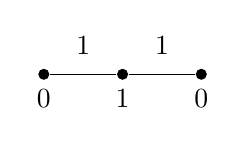
\begin{tikzpicture}
      \coordinate[vertex,label=below:$0$] (v1);
      \coordinate[vertex,right of=v1,label=below:$1$] (v2);
      \coordinate[vertex,right of=v2,label=below:$0$] (v3);
      \begin{scope}
        \draw (v1) -- node[label=$1$]{} (v2);
        \draw (v2) -- node[label=$1$]{} (v3);
      \end{scope}
    \end{tikzpicture} \qquad
    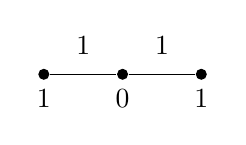
\begin{tikzpicture}
      \coordinate[vertex,label=below:$1$] (v1);
      \coordinate[vertex,right of=v1,label=below:$0$] (v2);
      \coordinate[vertex,right of=v2,label=below:$1$] (v3);
      \begin{scope}
        \draw (v1) -- node[label=$1$]{} (v2);
        \draw (v2) -- node[label=$1$]{} (v3);
      \end{scope}
    \end{tikzpicture} \qquad
    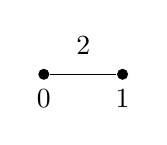
\begin{tikzpicture}
      \coordinate[vertex,label=below:$0$] (v1);
      \coordinate[vertex,right of=v1,label=below:$1$] (v2);
      \begin{scope}
        \draw (v1) -- node[label=$2$]{} (v2);
      \end{scope}
    \end{tikzpicture} \]
  The first two graphs correspond to $\Sigma = \Sigma_1 \cup \Sigma_2$
  where $f|_{\Sigma_i}$ is an isomorphism $\Sigma_i \cong \bP^1$: each
  edge of degree $1$ is an uncontracted component, and by stability
  there cannot be any contracted components. In the first graph,
  $f(\Sigma_1 \cap \Sigma_2) = q_1$, and in the second, $f(\Sigma_1
  \cap \Sigma_2) = q_0$. Finally, the third graph is irreducible and
  isomorphic to $\bP^1$; choosing coordinates, we can write $f(z_0,
  z_1) = (z_0^2, z_1^2)$.
\end{example}

\begin{definition} \label{def:flag-of-fixed-graph}
  A {\bf flag} $F$ of a fixed graph is an incident edge-vertex pair
  $(v, e)$. Put $i(F) \coloneqq v$, and let $j(F)$ denote the other
  vertex of the edge $e$. Define
  \[ \omega_F \coloneqq \frac{\lambda_{i(F)} - \lambda_{j(F)}}{d_e} \in H^2_{\bT}, \]
  which is the weight of the $\bT$-action on the tangent space of the
  component $C_e$ at the preimage $p_F$ of $q_{i_v}$. Let $e_F$ be the
  first Chern class of the line bundle on $\cnj\cM_\Gamma$ whose fiber
  is the cotangent space to the component associated to $v$ at $p_F$.
  The flags associated to a fixed vertex $v$ are often denoted
  $F_1(v), \ldots, F_k(v)$.
\end{definition}

\begin{theorem}[{\cite[Section 3.3]{Kontsevich1995}}] \label{thm:euler-class-fixed-graph}
  The equivariant Euler class of the normal bundle $N_\Gamma$ is given
  by
  \[ e(N_\Gamma) = e_\Gamma^F e_\Gamma^v e_\Gamma^e \]
  where the contributions from flags, vertices, and edges are
  \begin{align*}
    e_\Gamma^F &\coloneqq \prod_{n(i(F)) \ge 3} (\omega_F - e_F) \Big/ \prod_{j \neq i(F)} (\lambda_{i(F)} - \lambda_j) \\
    e_\Gamma^v &\coloneqq \prod_v \prod_{j \neq i_v} (\lambda_{i_v} - \lambda_j) \prod_{\substack{\val(v) = 2\\S_v = \emptyset}} (\omega_{F_1(v)} + \omega_{F_2(v)}) \Big/ \prod_{\substack{\val(v) = 1\\S_v = \emptyset}} \omega_{F(v)} \\
    e_\Gamma^e &\coloneqq \prod_e \frac{(-1)^{d_e} (d_e!)^2 (\lambda_i - \lambda_j)^{2d_e}}{d_e^{2d_e}} \prod_{\substack{a+b=d_e\\k \neq i,j}} \left(\frac{a\lambda_i + b\lambda_j}{d_e} - \lambda_k\right).
  \end{align*}
\end{theorem}

\begin{proof}[Proof sketch]
  We perform these calculations on $\cnj\cM_\Gamma$ rather than
  $\cnj\cM_\Gamma/A_\Gamma$; when applying localization we therefore
  must divide by $|A_\Gamma|$. The deformation long exact sequence
  \eqref{eq:deformation-long-exact-sequence} terminates early because
  $\bP^r$ is convex by \ref{thm:projective-spaces-are-convex}:
  \[ 0 \to \Aut(\Sigma, p_1, \ldots, p_n) \to \Def(f) \to \Def(\Sigma, p_1, \ldots, p_n, f) \to \Def(\Sigma, p_1, \ldots, p_n) \to 0. \]
  Consider the pullback of this sequence to $\cnj\cM_\Gamma$. For $V$
  a vector bundle, write $V^{\text{fix}}$ for its fixed (weight zero)
  part, and $V^{\text{mov}}$ for its {\bf moving} (weight nonzero)
  part. Then $\Def(\Sigma, p_1, \ldots, p_n, f)$ is the pullback of
  $T\cnj\cM_{0,n}(\bP^r, d)$, and contains $\Def(\Sigma, p_1, \ldots,
  p_n, f)^{\text{fix}}$, the tangent bundle of $\cnj\cM_\Gamma$, and
  $\Def(\Sigma, p_1, \ldots, p_n, f)^{\text{mov}}$, the normal bundle
  $N_\Gamma$. Hence the deformation exact sequence gives
  \[ e(N_\Gamma) = e(\Def(\Sigma, p_1, \ldots, p_n, f)^{\text{mov}}) = \frac{e((\Def f)^{\text{mov}}) e((\Def(\Sigma, p_1, \ldots, p_n))^{\text{mov}})}{e((\Aut(\Sigma, p_1, \ldots, p_n))^{\text{mov}})}. \]
  So it suffices to determine the contributions of each term. We give
  a rough outline of the arguments.
  \begin{enumerate}
  \item ($\Aut(\Sigma, p_1, \ldots, p_n)$) The $\bT$-action on the
    infinitesimal automorphisms of $(\Sigma, p_1, \ldots, p_n)$ fixes
    the automorphisms of non-contracted components with at least two
    special points. So consider vertices $v$ of valency $1$, where
    there are non-fixed automorphisms corresponding to moving the
    point mapping to $q_{i_v}$; clearly the space of such
    automorphisms is $T_{p_F}\Sigma$ where $F = F(v)$ is the unique
    flag incident to $v$ (cf. \ref{def:flag-of-fixed-graph}). By
    definition, the weight corresponding to $v$ is $\omega_{F(v)}$.
  \item ($\Def(\Sigma, p_1, \ldots, p_n)$) There are two cases here
    for weight non-zero elements: deformations that move nodes
    connecting contracted components to non-contracted components, and
    nodes connecting two non-contracted components. In the first case,
    we are looking at flags $F$ with $n(i(F)) \ge 3$, and the tangent
    space to the non-contracted curve is weight $\omega_F$ while that
    of the contracted curve is weight $-e_F$, so each such $F$
    contributes $(\omega_F - e_F)$. In the second case, we are looking
    at vertices of valency $2$ with no markings, which contribute
    $(\omega_{F_1(v)} + \omega_{F_2(v)})$.
  \item ($\Def(f) = H^0(\Sigma, f^*T\bP^r)$) Take the normalization
    exact sequence \eqref{eq:normalization-exact-sequence}
    \[ 0 \to \cO_\Sigma \to \bigoplus_{\text{vertices } v} \cO_{\Sigma_v} \oplus \bigoplus_{\text{edges } e} \cO_{\Sigma_e} \to \bigoplus_{\text{flags } F} \cO_{i(F)} \to 0, \]
    tensor with $f^*(T\bP^r)$, and take cohomology to get
    \[ 0 \to H^0(\Sigma, f^*T\bP^r) \to \bigoplus_{\text{vertices } v} H^0(\Sigma_v, f^*T\bP^r) \oplus \bigoplus_{\text{edges } e} H^0(\Sigma_e, f^*T\bP^r) \to \bigoplus_{\text{flags } F} T_{p_{i(F)}} \bP^r \to 0. \]
    (Convexity ends this sequence.) Hence we have an expression for
    $H^0(\Sigma, f^*T\bP^r)$ in the representation-theoretic (or
    K-theoretic) sense, and it suffices to figure out the
    contributions from each of the terms. This is a lot more work, and
    results in $e_\Gamma^e$.
  \end{enumerate}
  The denominator of $e_\Gamma^F$ cancels with the first term of the
  numerator of $e_\Gamma^v$, and we have accounted for the rest of the
  terms.
\end{proof}

\begin{remark}
  More generally, the same kind of argument applies to
  $\cnj\cM_{g,n}(\bP^r, d)$, but now each fixed locus has a ``virtual
  normal bundle'' and there is a ``virtual localization formula''
  which leads to an even more complicated expression for
  $e(N_\Gamma^{\vir})$.
\end{remark}

\begin{remark}
  At this point we must be careful about how localization works for
  (smooth) stacks, since we are viewing $\cnj\cM_{0,n}(\bP^r, d)$ as
  the orbifold underlying the smooth stack. Everything still makes
  sense, but we must divide out by the automorphisms at each fixed
  point locus:
  \begin{equation} \label{eq:stacky-localization}
    \int_X \alpha = \sum_j \int_{F_j} \left(\frac{i_j^*(\alpha)}{a_j e(N_j)}\right)
  \end{equation}
  where $a_j$ is the order of the group occurring in a local chart at
  the generic point of $F_j$.
\end{remark}

\subsection{The Aspinwall--Morrison Formula}

One final aspect of Gromov--Witten theory we must understand is the
existence of {\bf multiple covers}. Given an irreducible rational
curve $f\colon \bP^1 \to X$ of degree $d$, we can always pre-compose
with an arbitrary degree $k$ map $g\colon \bP^1 \to \bP^1$ to get a
``new'' curve $f \circ g\colon \bP^1 \to X$ of degree $kd$,
contributing spurious positive-dimensional components to
$\cnj\cM_{0,n}(X, d)$. We focus on $X$ a Calabi--Yau $3$-fold.

\begin{definition}
  An embedding $\Sigma \to X$ where $X$ is a Calabi--Yau $3$-fold is
  {\bf rigid} if it has normal bundle $N\Sigma = \cO_{\bP^1}(-1)
  \oplus \cO_{\bP^1}(-1)$.
\end{definition}

\begin{example}
  The degree $1$ (genus $0$) Gromov--Witten invariant of $X$ is the
  number of rigid lines, which is known to be $2875$. Hence the degree
  $2$ invariant receives contributions from double covers of these
  $2875$ lines, i.e. even generically, $\cnj\cM_{0,0}(X, 2)$ has
  $2875$ components isomorphic to $\cnj\cM_{0,0}(\bP^1, 2)$.
\end{example}

\begin{theorem}[Aspinwall--Morrison formula] \label{thm:aspinwall-morrison-formula}
  Let $\Sigma \subseteq X$ be a rigidly embedded smooth rational curve
  of class $\beta$ in the Calabi--Yau $3$-fold $X$. Then the
  contribution of degree $d$ multiple covers of $\Sigma \cong \bP^1$
  to Gromov--Witten invariant $\inner{I_{0,0,d[\Sigma]}}$ of $X$ is
  $1/d^3$.
\end{theorem}

\begin{proof}
  We work in $\cnj\cM_{0,0}(\bP^1, d)$, which consists of degree $d$
  multiple covers of $\Sigma \cong \bP^1$. The contribution we want is
  the restriction of $[\cnj\cM_{0,0}(X, d[\Sigma])]^{\vir}$ to
  $\cnj\cM_{0,0}(\bP^1, d)$. Since $\cnj\cM_{0,0}(\bP^1, d)$ is
  non-singular, by \ref{ex:virtual-fundamental-class-nonsingular},
  this contribution is exactly $e(\Ob)$, where $\Ob$ is the
  obstruction bundle, with fibers $H^1(\Sigma, f^*TX)$. Hence we must
  compute $\int_{\cnj\cM_{0,0}(\bP^1, d)} e(\Ob)$. From the long exact
  sequence of $0 \to f^*T\Sigma \to f^*TX \to f^*N\Sigma \to 0$ and
  the vanishing of $H^1(\Sigma, f^*T\bP^1)$, we get
  \[ H^1(\Sigma, f^*TX) = H^1(\Sigma, f^*N\Sigma) = H^1(\Sigma, f^*(\cO_{\bP^1}(-1) \oplus \cO_{\bP^1}(-1))). \]
  To compute the integral, we use localization; however, we change the
  torus action on $\cO_{\bP^1}(-1) \oplus \cO_{\bP^1}(-1)$ to simplify
  the calculation. Restrict the torus to $\bT' \coloneqq \bC^* \times
  \{1\} \subset \bT = (\bC^*)^2$ and let $\hbar$ denote the
  restriction of $\lambda_0$ to $\bT'$. Put the $\bT'$-action
  \[ t \cdot (l(x_0, x_1), m(x_0, x_1)) \coloneqq (l(tx_0, x_1), m(x_0, t^{-1}x_1)), \quad l, m \in \cO_{\bP^1}(-1) \]
  on $\cO_{\bP^1}(-1) \oplus \cO_{\bP^1}(-1)$. Clearly the fixed point
  loci in $\cnj\cM_{0,0}(\bP^1, d)$ of $\bT'$ is the same as that of
  $\bT$. The claim is that if a fixed graph $\Gamma$ has more than one
  edge, then its contribution is $0$. If there is more than one edge,
  there must be at least one node. Let $f\colon \Sigma \to \bP^1$ be a
  generic point of $\cnj\cM_\Gamma$, and let $\{b_i\}$ be the node
  branches. Tensoring the normalization exact sequence
  \eqref{eq:normalization-exact-sequence} with $f^*(\cO_{\bP^1}(-1)
  \oplus \cO_{\bP^1}(-1))$ gives
  \[ 0 \to f^*(\cO_{\bP^1}(-1) \oplus \cO_{\bP^1}(-1)) \to \bigoplus_i (f|_{\Sigma_i})^*(\cO_{\bP^1}(-1) \oplus \cO_{\bP^1}(-1)) \to \bigoplus_i (f|_{b_i})^*(\cO_{\bP^1}(-1) \oplus \cO_{\bP^1}(-1)) \to 0, \]
  which gives a long exact sequence of cohomology beginning with
  \[ 0 \to \bigoplus_i H^0(b_i, (f|_{b_i})^*(\cO_{\bP^1}(-1) \oplus \cO_{\bP^1}(-1))) \to H^1(\Sigma, f^*(\cO_{\bP^1}(-1) \oplus \cO_{\bP^1}(-1)) \to \cdots. \]
  If $f(b_i) = q_1$, then $T'$ acts trivially on the first
  $(f|_{b_i})^*\cO_{\bP^1}(-1)$ factor in the $H^0$ term. Similarly,
  if $f(b_i) = q_0$, then $T'$ acts trivially on the second factor.
  Hence there are vanishing $\bT'$-weights in $\bigoplus_i H^0$, and
  therefore in $H^1$. Since the Euler class is the product of weights,
  $\Gamma$ has contribution zero. It therefore suffices to look at
  \[ \Gamma =
    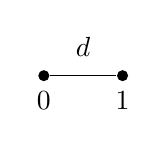
\begin{tikzpicture}
      \coordinate[vertex,label=below:$0$] (v1);
      \coordinate[vertex,right of=v1,label=below:$1$] (v2);
      \begin{scope}
        \draw (v1) -- node[label=$d$]{} (v2);
      \end{scope}
    \end{tikzpicture}, \quad
    A_\Gamma = \bZ/d\bZ, \quad f(z_0, z_1) = (z_0^d, z_1^d). \]
  It remains to find the weights of $i^*e(\Ob)$ and $e(N_\Gamma)$. The
  latter is easy: by \ref{thm:euler-class-fixed-graph},
  \begin{align*}
    e_\Gamma^F &= 1/((\hbar - 0)(0 - \hbar)) = -\hbar^{-2} \\
    e_\Gamma^v &= (\hbar - 0)(0 - \hbar) / ((\hbar/d - 0) (0 - \hbar/d)) = d^2 \\
    e_\Gamma^e &= \frac{(-1)^d (d!)^2 (\hbar - 0)^{2d}}{d^{2d}} = \frac{(-1)^d (d!)^2 \hbar^{2d}}{d^{2d}}.
  \end{align*}
  Hence $e(N_\Gamma) = (-1)^{d-1}(d!)^2 \hbar^{2d-2}/d^{2d-2}$. To
  compute $e(\Ob)$, take the usual cover $\{U_0, U_1\}$ for $\bP^1$,
  so that a basis for $H^1$ is given by the \v Cech cocycles
  $(z_0^{-k} z_1^{d-k}, 0)$ and $(0, z_0^{-k} z_1^{d-k})$ for $1 \le k
  \le d-1$. By the definition of the $\bT'$-action, $x_0, x_1 \in
  H^0(\bP^1, \cO_{\bP^1}(-1))$ have weights $\hbar$ and $0$, so since
  $x_i = z_i^d$ via $f$, we know $z_0, z_1$ have weights $\hbar/d$ and
  $0$. The $1$-cocycles therefore have weights $-k\hbar/d$ and
  $(d-k)\hbar/d$, and the Euler class is $(-1)^{d-1} ((d-1)!)^2
  (\hbar/d)^{2d-2}$. Hence
  \[ \int_{\cnj\cM_{0,0}(\bP^1, d)} e(\Ob) = \frac{1}{d}\frac{(-1)^{d-1} ((d-1)!)^2 \hbar^{2d-2}/d^{2d-2}}{(-1)^{d-1} (d!)^2 \hbar^{2d-2}/d^{2d-2}} = \frac{1}{d^3}, \]
  where the extra $1/d$ comes from the automorphism group $A_\Gamma =
  \bZ/d\bZ$ (see \eqref{eq:stacky-localization}).
\end{proof}

\chapter{Mirror Symmetry}

Using all the machinery from Gromov--Witten theory that we have
developed so far, we can give a mathematically precise statement of
mirror symmetry in special cases.

\section{Complex and K\"ahler Moduli}

The first step to a mathematically rigorous statement of mirror
symmetry is to understand more fully the complex and K\"ahler moduli.

\subsection{Hodge Theory and Complex Moduli}

\begin{definition}
  When the Hodge decomposition exists, $H^k(X; \bC) \cong
  \bigoplus_{p+q=k} H^{p,q}(X)$ (where $H^{p,q}(X) =
  \cnj{H^{q,p}(X)}$) along with the integer lattice from $H^k(X; \bZ)$
  form a {\bf Hodge structure of weight $k$}. Equivalently, we can
  specify the {\bf Hodge filtration} $F^p(X) \coloneqq \bigoplus_{a
    \ge p} H^{a,k-a}(X)$, which satisfies $H^{p,q}(X) = F^p(X) \cap
  \cnj{F^q(X)}$. The pairing $Q(\alpha, \beta) = (-1)^{\binom{k}{2}}
  \int_X \omega^{n-k} \wedge \alpha \wedge \beta$ on $H^k(X; \bC)$
  gives a {\bf polarized Hodge structure}.
\end{definition}

\begin{definition}
  Let $\pi\colon \cX \to S$ a flat morphism of relative dimension $n$
  with $S$ smooth, and put $X_t \coloneqq \pi^{-1}(t)$ for $t \in S$.
  Then $H^k(X_t; \bC)$ fit together into a locally free sheaf $\cF^0
  \coloneqq R^k\pi_*\bC \otimes \cO_S$, and $F^p(X_t)$ a locally free
  subsheaf $\cF^p$. The {\bf Gauss--Manin connection} $\nabla$ is a
  flat connection on $\cF^0$. Set $\cH \coloneqq \cF^0$, which has the
  locally constant subsheaf $\cH_{\bC} \coloneqq R^k\pi_*\bC$, which
  has the subsheaf of integer cohomology $\cH_{\bZ} \coloneqq
  R^k\pi_*\bZ$. The tuple $(\cH, \nabla, \cH_{\bZ}, \cF^\bullet)$ is a
  {\bf variation of Hodge structure}.
\end{definition}

\begin{remark}
  For our purposes, $k = \dim(X_t)$, i.e. we care only about the
  middle cohomology (cf. \ref{def:hodge-bundle}).
\end{remark}

\begin{definition} \label{def:picard-fuchs-equations}
  Let $p \in S$ and $z_1, \ldots, z_r$ be local analytic coordinates.
  Let $\cD \coloneqq \bC\{z_1, \ldots, z_r\}[\di_1, \ldots, \di_r]$
  where $\bC\{z_1, \ldots, z_r\}$ is the ring of convergent power
  series. Then the Gauss--Manin connection $\nabla$ gives an
  $\cO_S$-homomorphism $\phi(X_1\cdots X_t) \coloneqq \nabla_{X_1}
  \cdots \nabla_{X_t} \Omega(t)$ for a fixed local section of $\cF^0$,
  i.e. $\cF^0$ has a $\cD$-module structure. The kernel $\ker \phi$ is
  the {\bf Picard--Fuchs ideal}, and the equations $D \cdot y = 0$ for
  $D \in I$ are the {\bf Picard--Fuchs equations} (cf.
  \ref{thm:picard-fuchs-equation}). It is easy to show that periods of
  $\Omega(t)$ are solutions.
\end{definition}

\begin{definition}
  Let $\pi\colon \cX \to S$ be a smooth family with a completion
  $\tilde\pi\colon \tilde \cX \to \tilde S$ where $\tilde S$ is a
  smooth compactification with {\bf boundary divisor} $D = \bigcup_i
  D_i \coloneqq \tilde S \setminus S$. The extension $\tilde \nabla$
  of the Gauss--Manin connection $\nabla$ may pick up singularities
  (regular singular points). If $\gamma_j$ is a loop around the
  boundary divisor $D_j$, let $\cT_j\colon H^n(X_t; \bC) \to H^n(X_t;
  \bC)$ denote the {\bf monodromy transformation} (which, up to
  conjugation, only depends on $\gamma_j$) given by lifting a
  cohomology class $\eta = \eta(0) \in H^n(X_t; \bC)$ to a
  $\nabla$-flat section $\eta(u) \in H^n(X_{\gamma_j(u)}; \bC)$ and
  setting $\cT_j(\eta) \coloneqq \eta(1)$.
\end{definition}

\begin{theorem}[Monodromy theorem] \cite[Theorems I', II']{Landman1973}
  For some integer $m \ge 0$, we have $(\cT_j^m - I)^{n+1} = 0$, i.e.
  $\cT_j$ is {\bf quasi-unipotent}.
\end{theorem}

From now on, suppose that the monodromy is unipotent and we are at $p
\in \tilde S$ with local coordinates $z_1, \ldots, z_r$ such that $D =
\di \tilde S$ is given by $z_1 \cdots z_r = 0$ and $p$ is at $z=0$.
Let $N_j \coloneqq \log \cT_j$. The idea is to extend the relevant
Hodge theoretic structures from $S$ to $\tilde S$.

\begin{theorem}[Nilpotent orbit theorem]
  The bundles $\cF^p$ over $S$ extend canonically to $\tilde \cF^p$
  over $\tilde S$, giving the {\bf limiting Hodge filtration}
  $\cF^\bullet_{\text{lim}}$. This extension is given by
  \[ s \in \cF^0 \mapsto \exp\bigg(-\frac{1}{2\pi i} \sum_j \log(z_j) N_j\bigg)s \in \tilde \cF^0. \]
  Furthermore, $\nabla_{z_j \di_j} = -\frac{1}{2\pi i} N_j$, and
  induces a linear map $F^p_{\text{lim}}/F^{p+1}_{\text{lim}} \to
  F^{p-1}_{\text{lim}}/F^p_{\text{lim}}$.
\end{theorem}

\begin{definition}
  Let $N \coloneqq \sum_j a_j N_j$ for $a_j > 0$, acting on $H^n(X_t;
  \bC)$. The {\bf monodromy weight filtration} $W_\bullet$ is given by
  \[ W_0 \coloneqq \im N^n, \quad W_1 \coloneqq \im N^{n-1} \cap \ker N, \quad W_2 \coloneqq \im N^{n-2} \cap \ker N + \im N^{n-1} \cap \ker N^2, \quad \ldots, \]
  such that $N(W_k) \subset W_{k-2}$ and $N^k$ induces an isomorphism
  $W_{n+k}/W_{n+k-1} \cong W_{n-k}/W_{n-k-1}$. In addition,
  $F^\bullet_{\text{lim}}$ induces a weight $k$ Hodge structure on
  $W_k/W_{k-1}$. The pair $(W_\bullet, F^\bullet_{\text{lim}})$ is a
  {\bf mixed Hodge structure}.
\end{definition}

\begin{definition}
  Fix a Calabi--Yau $3$-fold $X$ with $1$-dimensional complex moduli
  space $S$. Let $p \in \di \tilde S$ have {\bf maximally unipotent
    monodromy}, i.e. $\cT\colon H^3(X; \bC) \to H^3(X; \bC)$ satisfies
  $(\cT - I)^3 \neq 0$. Since $h^{2,1}(X) = 1$, we have $h^3(X) = 4$,
  so let $g_0, \ldots, g_3$ be a basis for $H^3(X; \bC)$ such that
  \[ \cT = \begin{pmatrix} 1 & 1 & 0 & 0 \\ 0 & 1 & 1 & 0 \\ 0 & 0 & 1 & 1 \\ 0 & 0 & 0 & 1 \end{pmatrix}. \]
  Let $\gamma_i$ be the homology class dual to $g_i$, and $y_j
  \coloneqq \int_{\gamma_j} \Omega$ be the {\bf periods} of a local
  basis $\Omega$ of $\tilde \cF^3$.
\end{definition}

\begin{corollary}
  Any $g \in H^3(X; \bC)$ extends to a multiple-valued flat section
  $g(z) \in \tilde\cF^0$, and the section $\exp(\frac{-\log z}{2\pi i}
  N) g(z)$ is single-valued and analytic at $z = 0$. In particular,
  $g_0(z)$ and therefore $y_0$ is single-valued and analytic at $z =
  0$.
\end{corollary}

\begin{proof}
  Note that $\cT(g_0) = g_0$ by the choice of basis $\{g_i\}$, so
  $N(g_0) = 0$. It follows that $\exp(\frac{-\log z}{2\pi i} N) g_0(z)
  = g_0(z)$. But $y_0 = \inner{g_0(z), \Omega(z)}$. (We can also get
  the asymptotics $y_i \sim c(\frac{\log z}{2\pi i})^i$ as $z \to 0$
  using that $\cT(g_i) = g_i + g_{i-1}$.)
\end{proof}

\begin{proposition}
  Let $z$ be the local coordinate at a boundary point of the
  $1$-dimensional complex moduli space $S$, and write $\delta =
  z\di_z$. If $\Omega$ is a local section of $\cF^0$ with
  Picard--Fuchs equation
  \[ \delta^4 y + f_1(z) \delta^3 y + f_2(z) \delta^2 y + f_3(z) \delta y + f_4(z) y = 0, \]
  (whose {\bf indicial equation} just has $\delta$ replaced with a
  variable $\lambda$) then the monodromy $\cT$ is:
  \begin{enumerate}
  \item unipotent iff the roots of the indicial equation are all
    integers;
  \item maximally unipotent iff the indicial equation is $(\lambda -
    l)^4 = 0$ for some $l \in \bZ$.
  \end{enumerate}
\end{proposition}

\begin{definition} \label{def:maximally-unipotent-boundary-point}
  Let $X$ be a $d$-dimensional Calabi--Yau, and $S$ the complex moduli
  space of $X$. Again let $\tilde S$ be a compactification and $D$ the
  boundary divisor. The point $p \coloneqq D_1 \cap \cdots \cap D_r$
  is a {\bf maximally unipotent boundary point} if:
  \begin{enumerate}
  \item the monodromies $\cT_j$ are all unipotent;
  \item if $N_j \coloneqq \log \cT_j$, the monodromy weight filtration
    $W_\bullet$ determined by $N \coloneqq \sum_i a_i N_i$ has $\dim
    W_0 = \dim W_1 = 1$ (i.e. unique holomorphic solution to
    Picard--Fuchs at $p$) and $\dim W_2 = 1 + r$ (i.e. $r$ other
    independent solutions with logarithmic singularities at $p$);
  \item if $g_0, \ldots, g_r$ is a basis of $W_2$ such that $g_0$
    spans $W_0$, then the matrix $(m_{ij})$ given by $N_i(g_j) =
    m_{ij}g_0$ is invertible.
  \end{enumerate}
  The last condition allows us to change to the basis $g_k' \coloneqq
  \sum_j g_j m^{jk}$, where $N_j(g_k') = \delta_{jk} g_0$, so that
  locally, $y_k = y_0 \frac{\log z_k}{2\pi i} + \text{holomorphic}$.
\end{definition}

\subsection{K\"ahler Moduli and the Mirror Map}

In this subsection we shall define the K\"ahler moduli space and, in
it, the analogues of maximally unipotent boundary points, called large
radius limit points. For this purpose we will also need to compactify
parts of the K\"ahler moduli space.

\begin{definition}
  Let $X$ be a projective orbifold with $h^{2,0}(X) = 0$. The {\bf
    K\"ahler cone} is the subset $K(X) \subset H^2(X; \bR) =
  H^{1,1}(X; \bR)$ of all K\"ahler classes. The {\bf complexified
    K\"ahler space} is
  \[ K_{\bC}(X) \coloneqq \{\omega \in H^2(X; \bC) : \im \omega \in K(X)\}/\im H^2(X; \bZ). \]
  The {\bf complexified K\"ahler moduli space} is
  $\cKM(X) \coloneqq K_{\bC}(X)/\Aut(X)$.
\end{definition}

\begin{definition} \label{def:large-radius-limit-point}
  Fix a maximal dimension simplicial cone $\sigma$ in $H^2(X; \bR)$
  with interior $\Int \sigma$ lying in $K(X)$. Define
  \[ D_\sigma \coloneqq (H^2(X; \bR) + i\Int \sigma)/\im H^2(X; \bZ) \subset K_{\bC}(X). \]
  Suppose $\sigma$ is generated by a basis $T_1, \ldots,T_r$ of
  $H^2(X; \bZ)$ mod torsion, i.e. $\Int \sigma = \{\sum_i t_iT_i : t_i
  > 0\}$, which gives an isomorphism between $D_\sigma$ and the open
  $r$-simplex $(\Delta^*)^r$ via
  \[ t_1T_1 + \cdots + t_rT_r \mapsto (q_1, \ldots, q_r) \coloneqq (e^{2\pi i t_1}, \ldots, e^{2\pi i t_r}). \]
  Compactifying, $\tilde D_\sigma \cong \Delta^r$, the closed
  $r$-simplex. The distinguished boundary point $0 \in \Delta^r$ is a
  {\bf large radius limit point} since an $\omega \in H^2(X; \bR) +
  i\Int \sigma$ with large imaginary part has image close to $0$. Each
  large radius limit point therefore has canonical {\bf coordinates}
  $(q_1, \ldots, q_r)$ as defined above.
\end{definition}

Now it is time to write down the local isomorphism, called the {\bf
  mirror map}, linking the coordinates of a large radius limit point
in $\cnj\cKM(X^\circ)$ with the coordinates of a maximally unipotent
boundary point in $\cnj\cM(X)$. For the remainder of this subsection,
$X$ is a Calabi--Yau $d$-fold.

\begin{definition} \label{def:mirror-coordinates}
  Fix a maximally unipotent boundary point $p$ in $\cnj\cM(X)$. From
  \ref{def:maximally-unipotent-boundary-point}, let $g_0, \ldots, g_r$
  be a basis for $W_2 \subset H^d(X)$, and $m_{ij}$ be the matrix
  given by $N_i(g_j) = m_{ij}g_0$. Define holomorphic {\bf mirror
    coordinates}
  \[ \frac{1}{2\pi i} \log q_k \coloneqq \frac{1}{\inner{g_0, \Omega}} \sum_{j=1}^r \inner{g_j, \Omega} m^{jk} \]
  in a neighborhood of the maximally unipotent boundary point $p$.
\end{definition}

\begin{remark}
  By the definition \ref{def:picard-fuchs-equations} of the
  Picard--Fuchs equations, the periods $y_i \coloneqq \int_{\gamma_i}
  \Omega = \inner{g_i, \Omega}$ are solutions, and in particular $y_0$
  is the unique (up to a constant) solution holomorphic at $p$. If we
  write $y_k \coloneqq \sum_{j=1}^r \inner{g_j, \Omega} m^{jk}$, then
  $y_k$ is also a solution to the Picard--Fuchs equations. Then
  \[ y_k = y_0 (\log(z_k)/2\pi i) + \tilde{y}_k \implies q_k = z_k \exp(2\pi i \tilde y_k/y_0), \]
  where $\tilde y_k$ is holomorphic at $p$.
\end{remark}

\begin{definition}
  Let $X^\circ$ be the mirror of $X$. Choose a subdivision $\Sigma_+$
  of the cone $K_+$, which gives a smooth partial compactification
  $\cnj\cKM(X^\circ)$. Each cone $\sigma \in \Sigma_+$ gives a large
  radius limit point. Taking $p$ to be a maximally unipotent boundary
  point in $\cnj\cM(X)$, the {\bf mirror map} in the canonical
  coordinates of \ref{def:large-radius-limit-point} is given by
  \[ M\colon \cnj\cM(X) \to \cnj\cKM(X^\circ), \quad p \mapsto (q_1(p), \ldots, q_r(p)) \in \cnj\cKM(X^\circ). \]
  Hence the mirror map is specified by two pieces of data:
  \begin{enumerate}
  \item the mirror coordinates $q_1, \ldots, q_r$, and
  \item the choice of generators $T_1, \ldots, T_r \in H^2(X^\circ)$
    for the cone $\sigma$, which gives the canonical coordinates
    around the large radius limit point.
  \end{enumerate}
\end{definition}

\begin{remark}
  For the mirror map $M$ to actually be a local isomorphism, we must
  \begin{enumerate}
  \item choose the classes $g_0, \ldots, g_r$ of $W_2$ correctly so
    that the coordinates $q_i$ are well-defined, and
  \item pick the large radius limit point and maximally unipotent
    boundary point in ``compatible'' compactifications of their moduli
    spaces.
  \end{enumerate}
  We shall now see what ``correctly'' means for the first point.
\end{remark}

\begin{conjecture}[Integrality conjecture] \label{def:integrality-conjecture}
  Pick a {\bf $\bZ$-basis} for the monodromy weight filtration, i.e. a
  choice $g_0 \in W_0 \cap H^d(X; \bZ)$ and $g_1, \ldots, g_r \in W_2
  \cap H^d(X; \bZ)$ such that they span as a $\bZ$-basis. Then the
  integer matrix $(m_{ij})$ defined by $N_i(g_j) = m_{ij} g_0$ is
  invertible.
\end{conjecture}

\begin{corollary}
  Pick two $\bZ$-bases $g_0, \ldots, g_r$ and $g_0', \ldots, g_r'$
  related by $g_j' = \sum_{k=0}^r c_{jk} g_k$. Then the respective
  mirror coordinates $q_k'$ and $q_k$ are actually equal.
\end{corollary}

\begin{proof}
  Via such a change of coordinates, we have
  \[ q_k' = \exp(2\pi i c^{k0}/c_{00}) q_k, \quad c^{k0} \coloneqq \sum_{j=1}^r c_{j0} (m')^{jk}. \]
  But $c_{00} = \pm 1$, and $c^{k0} \in \bZ$. Hence $q_k' = q_k$.
\end{proof}

We will always assume the integrality conjecture from now on, because
it gives us a unique choice of mirror coordinates $q_1, \ldots, q_k$.
The conjecture has been verified for the quintic threefold
\cite{Morrison1993}.

\begin{proposition} \cite[Proposition 5.6.1]{Cox1999} \label{thm:picard-fuchs-equation-in-monodromy-coordinates}
  Suppose $X$ is a Calabi--Yau $3$-fold and we are at a maximally
  unipotent boundary point satisfying the integrality conjecture. Let
  $q$ denote the mirror coordinate and $\delta \coloneqq 2\pi i q
  \di_q$. Then there exist coordinates $e_0, e_1, e_2, e_3$ such that
  $\nabla_\delta$, the Gauss--Manin connection, and the Picard--Fuchs
  equation are
  \[ \nabla_\delta = \begin{pmatrix} 0 & 0 & 0 & 0 \\ 1 & 0 & 0 & 0 \\ 0 & Y & 0 & 0 \\ 0 & 0 & 1 & 0 \end{pmatrix}, \quad \nabla_\delta^2 \left(\frac{\nabla_\delta^2 \Omega}{Y}\right) = 0, \quad Y \coloneqq -\int_X \Omega \wedge \nabla_\delta^3\Omega. \]
\end{proposition}

\subsection{A-Model Variation of Hodge Structure}

Throughout this section, $X$ is a Calabi--Yau $d$-fold for $d \ge 3$
unless otherwise stated. Let $T_0 = 1, T_1, \ldots, T_m$ be a basis of
$H^*(X; \bQ)$, and $T_1, \ldots, T_r$ span $H^2(X; \bQ)$.

\begin{lemma}
  If $\delta \coloneqq \sum_{i=1}^r t_i T_i$ and $\epsilon \coloneqq
  t_0T_0 + \sum_{i=r+1}^m t_i T_i$, then
  \[ T_i *_{\text{big}} T_j = \sum_{\vec n = 0}^\infty \sum_\beta \frac{1}{\vec n!} \inner{I_{0,n+3,\beta}}(T_i, T_j, T_k, \epsilon^{\vec n}) e^{\int_\beta \delta} q^\beta T^k. \]
  Hence $T_i *_{\text{small}} T_j = T_i *_{\text{big}} T_j|_{\delta =
    \epsilon = 0}$.
\end{lemma}

\begin{definition} \label{def:restricted-big-quantum-product}
  We would like to study the K\"ahler moduli space, which is
  restricted to $H^2(X)$, i.e. $t_0 = t_{r+1} = \cdots = t_m = 0$.
  Hence define the {\bf restricted big quantum product} $T_i *
  T_j|_{\epsilon = 0}$. If we set $\omega = 0$ and let $\vec q^\beta
  \coloneqq e^{\int_\beta \delta} = \prod_{i=1}^r q_i^{\int_\beta
    T_i}$, then
  \[ T_i * T_j|_{\epsilon = 0} = \sum_\beta \inner{I_{0,3,\beta}}(T_i,T_j,T_k) \vec q^{\beta} T^k, \]
  which agrees with $*_{\text{small}}$ under a homomorphism of
  coefficient rings sending $\vec q^\beta$ to $q^\beta$.
  Alternatively, they agree as formal power series in the $t_i$ by
  setting $\omega = (1/2\pi i) \sum_{i=1}^r t_i T_i$.
\end{definition}

\begin{definition}
  Let $\cH \coloneqq H^*(X; \bC) \times K_{\bC}(X)$, which is the
  analogue of the Hodge bundle over complex moduli. The {\bf A-model
    connection} $\nabla$ on $\cH$ is given by
  \[ \nabla_{t_i}(T_j) \coloneqq \frac{1}{2\pi i} (T_i *_{\text{small}} T_j). \]
  From the preceding remark and the fact that the Dubrovin connection
  (associated to the Gromov--Witten potential) is flat (cf.
  \ref{thm:dubrovin-connection-is-flat}), we know $\nabla$ is flat.
\end{definition}

\begin{proposition}
  Using the notation of \ref{def:large-radius-limit-point}, the
  A-model connection has regular singular points along $\Delta^r
  \setminus D_\sigma$. Let $\cT_j$ be the monodromy determined by a
  loop around the origin in the $j$-th factor of $(\Delta^*)^r$. Then
  $\cT_j$ is unipotent, and up to conjugacy, $N_j \coloneqq \log
  \cT_j$ is determined by cup product with $-T_j$.
\end{proposition}

\begin{definition}
  Using this proposition we can show that the canonical extension
  $\tilde\cH$ to $\Delta^r$ can be naturally identified with the
  trivial bundle $H^*(X; \bC) \times \Delta^r$. We can use this to
  obtain an integral structure on $\cH$. A $\nabla$-flat section $s$
  is {\bf integral} if $\tilde s \coloneqq \exp(-2\pi i\sum_j t_j
  N_j)s$ is an integral class in $H^*(X; \bC)$ at the point $p \in
  \Delta^r$. Let $\cH_{\bZ}$ denote the locally constant sheaf of such
  sections; tensoring with $\bR$ gives $\cH_{\bR}$.
\end{definition}

\begin{corollary}
  The monodromy weight filtration of $\nabla$ at $0 \in \Delta^r$ is
  given by $W_i = \bigoplus_{j \ge 2d-i} H^j(X; \bC)$.
\end{corollary}

\begin{proof}
  Recall that $W_\bullet$ is determined by $N \coloneqq \sum_{j=1}^r
  a_j N_j$, i.e. cupping with the K\"ahler class $\omega =
  \sum_{j=1}^r a_j T_j$. Now use that $- \cup \omega^k$ is an
  isomorphism by hard Lefschetz.
\end{proof}

\begin{corollary}
  The A-model connection has maximally unipotent monodromy at $0 \in
  \Delta^r$.
\end{corollary}

\begin{proof}
  It suffices to check conditions 2 and 3 in
  \ref{def:maximally-unipotent-boundary-point}. Since $H^1(X; \bC) =
  0$, the previous corollary shows $\dim W_0 = \dim W_1 = h^{2d}(X) =
  1$. If $g_0 \in H^{2d}(X; \bC)$ is dual to a point and $g_i \in
  H^{2d-2}(X; \bC)$ is dual to $T_i$, then at the fiber over $0 \in
  \Delta^r$,
  \[ N_i(g_j) = -T_i \cup g_j = -g_0 \int_X T_i \cup g_j = -g_0 \delta_{ij}, \]
  and clearly $(\delta_{ij})$ is invertible.
\end{proof}

\begin{definition}
  Now we turn the A-model connection into a variation of Hodge
  structure. Let $X$ be a Calabi--Yau $d$-fold for $d \ge 3$, and set
  $F^p \coloneqq \bigoplus_{a\le d-p} H^{a,b}(X)$, giving a decreasing
  {\bf filtration} $H^*(X; \bC) = F^0 \supset F^1 \supset \cdots$.
  Define the subbundles $\cF^p \coloneqq F^p \times K_{\bC}(X) \subset
  \cH$ which give a filtration of $\cH$. Also define the {\bf
    intersection form}
  \[ S(\alpha, \beta) \coloneqq (-1)^{k(k+1)/2} \int_X \alpha \cup \beta, \quad \alpha \in H^k(X; \bC), \; \beta \in H^l(X; \bC), \]
\end{definition}

\begin{theorem} \cite[Theorem 8.5.11]{Cox1999}
  Let $X$ be a Calabi--Yau $d$-fold for $d \ge 3$. Then in a
  neighborhood $U$ of $0 \in \Delta^r$, $(\cH, \nabla, \cH_{\bZ},
  \cF^\bullet)$ is a variation of Hodge structure over $U \cap
  (\Delta^*)^r$ of weight $d$ polarized by $S$.
\end{theorem}

\begin{definition}
  We call $(\cH, \nabla, \cH_{\bZ}, \cF^\bullet)$ the {\bf A-variation
    of Hodge structure}. Let $\cH^{\text{middle}} \subset \cH$ denote
  the subbundle with fibers $\bigoplus_{p=0}^d H^{p,p}(X)$, the middle
  part of the Hodge decomposition of $H^*(X; \bC)$. By
  \ref{thm:small-quantum-product-is-hodge-compatible}, $\nabla$
  preserves $\cH^{\text{middle}}$, so let $\nabla^{\text{middle}}
  \coloneqq \nabla|_{\cH^{\text{middle}}}$. The remaining structures
  also restrict, to give the {\bf middle A-variation of Hodge
    structure} $(\cH^{\text{middle}}, \nabla^{\text{middle}},
  \cH_{\bZ}^{\text{middle}}, \cF^\bullet)$. The pairing $S$ restricts
  to $\cH^{\text{middle}}$, polarizing the middle A-variation.
\end{definition}

\section{Mathematical Mirror Pairs}

\subsection{Calabi--Yau 3-Folds}

Let's sum up the setting. We have two smooth Calabi--Yau $3$-folds $X$
and $X^\circ$, with $\cnj\cM(X)$ and $\cnj\cKM(X^\circ)$ being
suitably compatible compactifications of the complex moduli space
$\cM(X)$ and the K\"ahler moduli space $\cKM(X^\circ)$ respectively.
More precisely, we have
\begin{enumerate}
\item a maximally unipotent boundary point $p_0 \in \cnj\cM(X)$,
\item a large radius limit point $q_0 \in \cnj\cKM(X^\circ)$, and
\item a mirror map mapping a neighborhood of $p_0$ to a neighborhood
  of $q_0$.
\end{enumerate}
(We assume $X$ satisfies the integrality conjecture
\ref{def:integrality-conjecture}, so that the mirror map is specified
uniquely.) There are two variations of Hodge structure:
\begin{enumerate}
\item on $\cM(X)$ we have the Gauss--Manin connection
  $\nabla^{\text{GM}}$ and the Hodge filtration on the bundle $\cH^X$
  given by $H^3(V; \bC)$;
\item on $\cKM(X^\circ)$ we have the A-model connection
  $\nabla^{\text{middle}}$ and the Hodge filtration on the bundle
  $\cH^{X^\circ}$ given by $H^{\text{middle}}(X^\circ) \coloneqq
  \bigoplus_{p=0}^3 H^{p,p}(X^\circ)$.
\end{enumerate}
Their integral structures are denoted $\cH^X_{\bZ}$ and
$\cH^{X^\circ}_{\bZ}$ respectively. Furthermore, these variations of
Hodge structure are polarized:
\begin{enumerate}
\item since every class $\alpha \in H^3(X; \bC)$ is primitive,
  $Q(\alpha, \beta) \coloneqq -\int_X \alpha \cup \beta$ polarizes
  $(\cH^X, \nabla^{\text{GM}}, \cH^X_{\bZ}, \cF^\bullet)$;
\item on $\bigoplus_{p=0}^3 H^{p,p}(X)$, the form $S(\alpha, \beta)
  \coloneqq (-1)^p \int_X \alpha \cup \beta$ for $\alpha \in
  H^{p,p}(X)$ and $\beta \in H^{3-p,3-p}(X)$ polarizes
  $(\cH^{X^\circ}, \nabla^{\text{middle}}, \cH^{X^\circ}_{\bZ},
  \cF^\bullet)$.
\end{enumerate}
Finally, there are two distinguished sections for each Hodge bundle.
\begin{enumerate}
\item On $X$, the bundle $\cH^X$ has the section $g_0$, which is an
  integral generator of $W_0$ and is unique up to sign. Normalize the
  section $\Omega$ of $\cF^3$ by the factor $y_0 \coloneqq \inner{g_0,
    \Omega}$ to get another distinguished section $\Omega/y_0$. Note
  that $Q(\Omega/y_0, g_0) = 1$ by construction.
\item On $X^\circ$, the bundle $\cH^{X^\circ}$ has the section $[\pt]
  \in H^{3,3}(X^\circ; \bZ)$, which an integral generator of $W_0$.
  The other distinguished section is $1 = T_0 \in H^0(X, \bC)$, which
  generates $\cF^3$ and satisfies $S(1, [\pt]) = 1$.
\end{enumerate}

\begin{definition}
  In the setting presented above, $(X, X^\circ)$ is a {\bf
    (Hodge-theoretic) mirror pair} if the mirror map lifts to an
  isomorphism of $\cH^X$ and $\cH^{X^\circ}$ in neighborhoods of $p_0$
  and $q_0$. This isomorphism should preserve the polarized variations
  of Hodge structure and send the sections $\Omega/y_0$ and $g_0$ to
  the sections $1$ and $[\pt]$ respectively.
\end{definition}

It turns out mirror pairs have an equivalent characterization in terms
of correlation functions, and this characterization is what we want to
work with. Recall that the Yukawa couplings, i.e. {\bf B-model
  correlation functions}, are given by
\[ Y_{ijk} = -\int_X \tilde\Omega \wedge \nabla_i \nabla_j \nabla_k \tilde\Omega = Q(\tilde\Omega, \nabla_i \nabla_j \nabla_k \tilde\Omega) \]
where $\tilde\Omega \coloneqq \Omega/y_0$ is normalized (see
\ref{def:yukawa-coupling}). Similarly, the {\bf A-model correlation
  functions} are given by
\[ \inner{T_i, T_j, T_k} = \int_{X^\circ} T_i *_{\text{small}} T_j *_{\text{small}} T_k = S(1, \nabla_i \nabla_j \nabla_k 1). \]

\begin{theorem} \label{thm:mirror-pair-correlation-functions}
  Suppose $X$ satisfies the integrality conjecture. Then $(X,
  X^\circ)$ is a mirror pair iff, via the mirror map, $Y_{ijk} =
  \inner{T_i, T_j, T_k}$ for all $i,j,k$.
\end{theorem}

\begin{proof}[Proof sketch]
  One direction is trivial: if there is a local isomorphism of moduli
  spaces with $\tilde\Omega \mapsto 1$, $\nabla^{\text{GM}} \mapsto
  \nabla^{\text{middle}}$, and $Q \mapsto S$, then clearly the
  equality of correlation functions follows. Conversely, pick the
  basis $e_0 = \tilde\Omega, e_1, \ldots, e_r$ for $\cH^X$ and the
  basis $T_0 = 1, T_1, \ldots, T_r$ for $\cH^{X^\circ}$. Then clearly
  $e_i \mapsto T_i$ is a bundle isomorphism. It remains to check that
  this isomorphism preserves the Hodge structures. This is not hard,
  because Yukawa couplings fully determine the Gauss--Manin connection
  (cf. \ref{thm:picard-fuchs-equation-in-monodromy-coordinates}), and
  the A-model correlation functions fully determine the A-model
  connection (cf. \ref{def:dubrovin-connection}). A similar argument
  works for the polarizations and integral structures at $0 \in
  \Delta^r$.
\end{proof}

\begin{corollary}
  Let $\Phi^{GM}$ denote the (complex moduli) prepotential from
  \ref{def:gauss-manin-prepotential}, and $\Phi^{GW}$ the
  Gromov--Witten potential. If $X$ satisfies the integrality
  conjecture, then $(X, X^\circ)$ is a mirror pair iff $\Phi^{GM} =
  \Phi^{GW}$ up to quadratic terms in the coordinates $t_i$.
\end{corollary}

\begin{proof}
  Note that $Y_{ijk} = \di_i \di_j \di_k \Phi^{GM}$
  (\ref{def:yukawa-coupling}) and by the definition of the big quantum
  product, $\inner{T_i,T_j,T_k} = \di_i \di_j \di_k \Phi^{GW}$ (cf.
  \ref{def:big-quantum-product}). Hence, under the mirror map, we can
  directly compare potentials.
\end{proof}

\begin{example}[Quintic threefold]
  Set $X^\circ$ to be the quintic threefold and $X$ to be the
  quintic mirror of \ref{def:mirror-quintic}. Then according to
  \ref{thm:mirror-pair-correlation-functions}, mirror symmetry for
  $(X, X^\circ)$ is equivalent to the equality
  \[ 5 + \sum_{d=1}^\infty n_d d^3 \frac{q^d}{1 - q^d} = \frac{5}{(1 + 5^5z) y_0(z)^2} \left(\frac{q}{z} \frac{dz}{dq}\right)^3. \]
  Indeed, the left hand side is the correlation function
  $\inner{H,H,H}$ (cf.
  \eqref{eq:calabi-yau-threefold-three-point-function}) of the quintic
  threefold, and the right hand side is the normalized Yukawa coupling
  (cf. \eqref{eq:quintic-threefold-normalized-yukawa-coupling})
  expressed in the mirror map coordinate $q \coloneqq \exp(2\pi i
  \inner{g_1, \tilde\Omega})$. To see this, write $\delta \coloneqq q
  \di_q = (q/z) (dz/dq) z \di_z$, so that the normalized
  Yukawa coupling becomes
  \[ Y = -\int_{X^\circ} \tilde\Omega \wedge \nabla_\delta \nabla_\delta \nabla_\delta \tilde\Omega = \left(\frac{q}{z} \frac{dz}{dq}\right)^3 \int_{X^\circ} \tilde\Omega \wedge \nabla_{z\di_z} \nabla_{z \di_z} \nabla_{z \di_z} \tilde\Omega = \left(\frac{q}{z} \frac{dz}{dq}\right)^3 \frac{5}{(1 + 5^5z) y_0(z)^2}. \]
  These are the only correlation functions because $h^{1,1}(X^\circ) =
  h^{2,1}(X) = 1$.
\end{example}

\subsection{Toric 3-Folds}

\todo{Construct Batyrev dual}

\begin{conjecture}[Mirror conjecture for Toric $3$-folds]
  Fix a reflexive polytope $\Delta$ of dimension $d = 3$ and let
  $\Sigma$ and $\Sigma^\circ$ be maximal projective subdivisions of
  the normal fans of $\Delta$ and $\Delta^\circ$ respectively. Then
  the minimal Calabi--Yau toric hypersurface $V \subset X_\Sigma$ and
  its Batyrev dual $V^\circ \subset X_{\Sigma^\circ}$ form a mirror
  pair.
\end{conjecture}

\section{Givental's Mirror Theorem}

In \cite{Givental1996}, Givental states and proves a mirror theorem
for nef complete intersections in $\bP^n$. We follow \cite[Section
  11.2]{Cox1999}, which outlines a slightly different version of
Givental's proof.

\subsection{The Givental Connection and Flat Sections}

We need explicit expressions for flat sections of the A-model
connection. As usual, $X$ is a smooth projective variety, and let $T_0
= 1, T_1, \ldots, T_m$ be a homogeneous basis of $M \coloneqq H^*(X;
\bC)$ such that $T_1, \ldots, T_r$ span $H^2(X; \bQ)$.

\begin{definition}
  Let $X$ be a smooth projective variety and $*$ the big quantum
  product. Identify $\di_{t_i}$ with $T_i$ so that $T_pM \cong M$, and
  the Dubrovin connections $\nabla^\lambda$ are defined on the trivial
  bundle $H^*(X; \bC) \times M$. The {\bf Givental connection} on $TM$
  (formally) is given by
  \[ \nabla^g_i(a^j T_j) \coloneqq \hbar (\di_i a^j) T_j - a^j T_j * T_i \]
  where $\hbar$ is a formal parameter (later to be identified with a
  generator of $H^2_{\bC^*}$).
\end{definition}

\begin{remark}
  Formally, $\nabla^g = \hbar \nabla^{-\hbar^{-1}}$, so $\nabla^g$ is
  also flat, and flat sections exist.
\end{remark}

\begin{definition}
  Recall that $\gamma \coloneqq \sum_i t_i T_i$ and the $\psi$-classes
  of gravitational descendant invariants (see
  \ref{def:gravitational-descendant-invariants}). For each $a = 0,
  \ldots, m$, define the formal section
  \[ s_a \coloneqq T_a + \!\!\!\!\!\sum_{\substack{n \ge 0, \beta\\(n,\beta)\neq(0,0)}} \!\!\frac{1}{n!} \inner{T_a \cdot \frac{T_b}{\hbar - \psi_1} \cdot \gamma^n}_\beta T^b = T_a + \!\!\!\!\!\sum_{\substack{n \ge 0, \beta\\(n,\beta)\neq(0,0)}} \!\!\sum_{k \ge 0} \frac{\hbar^{-k-1}}{n!} \inner{T_a \cdot \tau_k(T_b) \cdot \gamma^n}_\beta T^b. \]
\end{definition}

\begin{proposition}
  The sections $s_a$ form a basis for $\nabla^g$-flat sections, i.e.
  they satisfy the {\bf quantum differential equation}
  \[ \nabla^g s_a = \hbar \di_i s_a - T_i * s_a = 0. \]
\end{proposition}

\begin{proof}
  The proof relies on the following {\bf topological recursion}
  relation:
  \[ \inner{\tau_{a_1}(\gamma_1)\tau_{a_2}(\gamma_2)\tau_{a_3}(\gamma_3)\prod_{i \in S} \tau_{d_i}(\eta_i)}_\beta = \sum_{\substack{\beta_1+\beta_2=\beta\\S_1 \sqcup S_2 = S}} \inner{\tau_{a_1-1}(\gamma_1) \prod_{i \in S_1} \tau_{d_i}(\eta_i) T_r}_{\beta_1} \inner{T^r \tau_{a_2}(\gamma_2)\tau_{a_3}(\gamma_3) \prod_{i \in S_2} \tau_{d_i}(\eta_i)}_{\beta_2} \]
  which follows from applying an analogue of the splitting lemma to
  the fact that for $\pi\colon \cnj\cM_{0,n}(X,\beta) \to \cM_{0,3}$,
  we have $\pi^*\bL_1 - \bL_1 = \sum_\Gamma D_\Gamma$ where the sum is
  over all boundary divisors separating $\{1\}$ from $\{2,3\}$. Then
  some symbol-pushing gives the quantum DE.
\end{proof}

\begin{remark}
  Since $T_0$ is the identity for $*$, we have $\hbar \di_0 s_a =
  s_a$, i.e. only a multiplicative factor $e^{t_0/\hbar}$ in $s_a$
  depends on $t_0$. So we often ignore $t_0$.
\end{remark}

\begin{remark}
  The topological recursion relation given in the above proof also
  shows that the genus $0$ descendant invariants are fully determined
  by genus $0$ Gromov--Witten invariants: just keep applying the
  relation until all the $\tau_{a_i}$ vanish.
\end{remark}

\begin{proposition}
  Let $T_1, \ldots, T_r$ be a basis for $H^2(X; \bQ)$, and $\delta
  \coloneqq \sum_{i=1}^r t_i T_i$. If we pass to small quantum
  cohomology via \ref{def:restricted-big-quantum-product}, then given
  $T \in H^*(X; \bC)$,
  \begin{equation} \label{eq:a-model-connection-flat-section}
    s(T) \coloneqq e^{\delta/\hbar} \cup T + \sum_{\beta \neq 0} \sum_{j=0}^m q^\beta \inner{\frac{e^{\delta/\hbar} \cup T}{\hbar - \psi_1} \cdot T_j}_\beta T^j
  \end{equation}
  is a flat (formal) section for the A-model connection $\nabla$.
\end{proposition}

\begin{proof}
  First restrict $s_a$ to $H^0(X; \bC) \oplus H^2(X; \bC)$, so that by
  \ref{def:restricted-big-quantum-product}, we can replace
  $*_{\text{big}}$ with $*_{\text{small}}$ under the homomorphism
  $\vec q^\beta \mapsto q^\beta$ of coefficient rings. Then do some
  symbol-pushing.
\end{proof}

\subsection{Givental's J Function}

Throughout this subsection we restrict $\nabla^g$ to act on the
trivial bundle $H^*(X; \bC) \times M$ over $M = H^0(X; \bC) \oplus
H^2(X; \bC)$, with basis $t_0, t_1, \ldots, t_r$.

\begin{definition}
  Let $s_a$ denote the $\nabla^g$-flat sections and $\inner{\cdot,
    \cdot}$ the usual intersection pairing. Define Givental's {\bf J
    function} $J \coloneqq \inner{s_j, 1}T^j$.
\end{definition}

\begin{theorem}
  Let $P(\hbar \di_t, e^t, \hbar)$ be a formal power series in the
  quantities $\hbar \di_0, \ldots, \hbar \di_r, e^{t_0}, \ldots,
  e^{t_r}, \hbar$, and let $P(T,q,0)$ denote the formal power series
  in $H^*(X; \cR)$ with coefficient ring $\cR \coloneqq \bC[[q_1,
      \ldots, q_r]]$ given by the substitutions $\hbar \di_j \mapsto
  T_j$ and $e^{t_j} \mapsto q_j$ and $\hbar \mapsto 0$. Then
  \[ P(\hbar \di_t, e^t, \hbar)J = 0 \implies P(T, q, 0) = 0 \text{ in small quantum cohomology}. \]
\end{theorem}

\begin{proof}
  Let $\tilde\nabla^g$ be the {\bf dual Givental connection}
  $\tilde\nabla^g_i(a^jT_j) \coloneqq \hbar (\di_i a^j)T_j + a^j T_i *
  T_j$. Since $T_0, \ldots, T_m$ are linearly independent, $PJ =
  P\inner{s_j, 1}T^j = 0$ implies $P\inner{s_j, 1} = 0$ for all $j$.
  Using the identities
  \[ \hbar \di_i \inner{G, H} = \inner{\nabla^g_i G, H} + \inner{G, \tilde\nabla^g_i H}, \quad \tilde\nabla^g_{i_1} \cdots \tilde\nabla^g_{i_k}1 = T_{i_1} * \cdots * T_{i_k} + \hbar A(T, q, \hbar) \]
  where $A$ is some formal series we don't care about, we get
  \[ 0 = P\inner{s_j, 1} = \inner{s_j, P(T,q,0)} + \hbar\inner{s_j, B(T, q, \hbar)} \]
  where $B$ is another formal series we don't care about, because upon
  setting $\hbar \mapsto 0$, the fact that the $s_j$ form a basis
  gives $P(T,q,0) = 0$.
\end{proof}

\begin{definition}
  A {\bf quantum differential operator} is a differential operator
  $P(\hbar \di_t, e^t, \hbar)$ satisfying the conditions of the
  preceding theorem.
\end{definition}

Givental's J function is not only important in studying quantum
differential operators, but also plays a crucial role in Givental's
proof of mirror symmetry for complete intersections in $\bP^n$. Hence
we need a more explicit expression for it.

\begin{lemma}
  Let $\delta \coloneqq \sum_{i=1}^r t_iT_i$ and $\vec q^\beta
  \coloneqq e^{\int_\beta \delta}$ as per
  \ref{def:restricted-big-quantum-product}. Let $\PD$ denote
  Poincar\'e duality. Then
  \begin{equation} \label{eq:givental-j-function}
  \begin{aligned}
    J &= e^{(t_0 + \delta)/\hbar} \bigg(1 + \sum_{\beta \neq 0} \vec q^\beta \inner{\frac{T_a}{\hbar - \psi_1}\cdot 1}_\beta T^a\bigg) \\
    &= e^{(t_0 + \delta)/\hbar} \bigg(1 + \sum_{\beta \neq 0} \vec q^\beta \PD^{-1}(\ev_1)_*\left(\frac{1}{\hbar - \psi_1} \cap [\cnj\cM_{0,2}(X,\beta)]^{\vir}\right)\bigg)
  \end{aligned}
  \end{equation}
\end{lemma}

\begin{proof}
  Plugging the expression \eqref{eq:a-model-connection-flat-section}
  for $s_a$ into the definition of $J$ and simplifying, we get
  \[ J = e^{t_0/\hbar}\bigg(e^{\delta/\hbar} + \sum_{\beta \neq 0} \vec q^\beta\inner{\frac{e^{\delta/\hbar} \cup T_a}{\hbar - \psi_1}\cdot 1}_\beta T^a\bigg). \]
  But $J$ is basis independent, so we can replace $\{T_a\}$ with any
  other basis, which does not even need to be homogeneous, e.g.
  $\{e^{-\delta/\hbar} \cup T_a\}$. This basis has dual basis
  $\{e^{\delta/\hbar} \cup T^a\}$, and substituting it in gives the
  first expression for $J$. The second expression follows from
  \[ \inner{\frac{T_a}{\hbar - \psi_1} \cdot 1}_\beta = \int_{[\cnj\cM_{0,2}(X,\beta)]^{\vir}} \frac{\ev_1^*(T_a)}{\hbar - \psi_1} = \int_X T_a \cup \PD^{-1}\bigg((\ev_1)_*\left(\frac{1}{\hbar - \psi_1} \cap [\cnj\cM_{0,2}(X,\beta)]^{\vir}\right)\bigg). \qedhere \]
\end{proof}

\begin{example}
  Let $X$ be a Calabi--Yau $3$-fold. Applying the degree axiom
  \ref{thm:gromov-witten-degree-axiom} to the equation
  \ref{eq:givental-j-function} for $J$,
  \begin{equation} \label{eq:givental-j-function-calabi-yau-threefold}
    J = e^{(t_0 + \delta)/\hbar} \bigg(1 + \sum_{\beta \neq 0} \vec q^\beta\bigg(\hbar^{-2}\sum_{a=1}^r \inner{\tau_1(T_a) \cdot 1}_\beta T^a + \hbar^{-3} \inner{\tau_2(1) \cdot 1}_\beta T^0\bigg)\bigg).
  \end{equation}
  By the string equation \eqref{eq:descendant-string-equation} and
  that $\sum_{a=1}^r (\int_\beta T_a) T^a$ is Poincar\'e dual to
  $\beta$, we abuse notation and write
  \[ J = e^{(t_0 + \delta)/\hbar} \bigg(1 + \hbar^{-2} \sum_{\beta \neq 0} N_\beta \vec q^\beta \beta - 2\hbar^{-3} \sum_{\beta \neq 0} N_\beta \vec q^\beta \pt\bigg) \]
  where $N_\beta \coloneqq \inner{I_{0,0,\beta}}$ are the
  Gromov--Witten invariants defining the instanton numbers (see
  \ref{ex:small-quantum-cohomology-calabi-yau-threefold}). Hence if we
  have an independent method of computing $J$, we get the $N_\beta$
  for free.
\end{example}

\begin{proposition} \cite[Proposition 10.3.4]{Cox1999} \label{thm:givental-j-function-calabi-yau-threefold}
  If $X$ is a Calabi--Yau $3$-fold, $\di_{t_i} \di_{t_j} J =
  \hbar^{-2} e^{(t_0+\delta)/\hbar} T_i * T_j$.
\end{proposition}

\begin{proof}[Proof sketch]
  First compute the Gromov--Witten potential $\Phi = (1/6)\int_X
  \delta^3 + \sum_{\beta \neq 0} N_\beta q^\beta$ for $X$. Then
  rewrite \eqref{eq:givental-j-function-calabi-yau-threefold} in terms
  of $\Phi$. Then differentiate, noting that $(\di_i \di_j \di_a \Phi)
  T^a = T_i * T_j$.
\end{proof}

\begin{definition}
  In preparation for Givental's mirror theorem for complete
  intersections in $\bP^n$, we consider a smooth complete intersection
  $X \subset \bP^n$ of $\ell$ hypersurfaces of degree $a_1, \ldots,
  a_\ell$, and write $\cV \coloneqq \bigoplus_{i=1}^\ell
  \cO_{\bP^n}(a_i)$ so that $X$ is the zero locus of some section of
  $\cV$. Let $H \in H^2(\bP^n)$ be the hyperplane class, and define
  the cohomology-valued formal function
  \begin{equation} \label{eq:givental-i-function}
    I_{\cV} = I_{\cV}(t_0, t_1, \hbar^{-1}) \coloneqq e^{(t_0 + t_1H)/\hbar} e(\cV) \sum_{d=0}^\infty e^{t_1d} \frac{\prod_{i=1}^\ell \prod_{m=1}^{a_i d} (a_i H + m\hbar)}{\prod_{m=1}^d (H + m\hbar)^{n+1}}.
  \end{equation}
  If $X = \bP^n$ so that $\cV$ is trivial, we write $I_{\bP^n}$.
\end{definition}

\begin{remark}
  This function $I_{\cV}$ may seem rather arbitrary. Indeed, this is
  because we are missing some background on hypergeometric DEs. The
  upcoming example \ref{ex:mirror-theorem-quintic-threefold} explains
  how $I_{\cV}$ is encoding precisely a basis of solutions for the
  Picard--Fuchs equations for the periods of $X$.
\end{remark}

\begin{definition} \label{def:givental-j-function}
  Let $J_X$ denote Givental's J function for $X$, to avoid confusion
  with the J function $J_{\cV}$ for $\cV$ which we shall define now
  (continuing with the notation of the previous definition). Let
  $\pi_{k+1}\colon \cnj\cM_{0,k+1}(\bP^n, d) \to \cnj\cM_{0,k}(\bP^n,
  d)$ forget the $(k+1)$-th marked point. Then there is a bundle
  $\cV_{d,k} \coloneqq (\pi_{k+1})_*\ev_{k+1}^*(\cV)$ with fiber
  $H^0(\Sigma, f^*(\cV))$ at $f\colon \Sigma \to \bP^n$ in
  $\cnj\cM_{0,k}(X, \beta)$. Using it, define another bundle
  $\cV_{d,k,i}'$ by the short exact sequence
  \begin{equation} \label{eq:exact-sequence-Vdki}
    0 \to \cV_{d,k,i}' \to \cV_{d,k} \to \ev_i^*(\cV) \to 0,
  \end{equation}
  i.e. consisting of sections of $\cV_{d,k}$ vanishing at the $i$-th
  marked point. Now by analogy with \eqref{eq:givental-j-function},
  define
  \begin{equation} \label{eq:givental-j-function-complete-intersection}
    J_{\cV} \coloneqq e^{(t_0 + t_1H)/\hbar} e(\cV) \left(1 + \sum_{d=1}^\infty e^{t_1d} (\ev_1)_*\left(\frac{e(\cV_{d,k,1}')}{\hbar - \psi_1}\right)\right).
  \end{equation}
\end{definition}

\begin{remark}
  When $\cV = 0$, i.e. $X = \bP^n$ (which is convex), we have $e(\cV)
  = 1$ and therefore that
  \[ J_{\cV} = e^{(t_0 + t_1H)/\hbar} \left(1 + \sum_{d=1}^\infty e^{t_1d} (\ev_1)_*\left(\frac{1}{\hbar - \psi_1}\right)\right) = J_{\bP^n}. \]
\end{remark}

\begin{lemma} \label{thm:hbar-expansion-of-j-function}
  $J_{\cV} = e^{(t_0 + t_1H)/\hbar} e(\cV) (1 + o(\hbar^{-1}))$.
\end{lemma}

\begin{proof}
  From the short exact sequence \eqref{eq:exact-sequence-Vdki}
  defining $\cV'_{d,k,i}$ and the projection formula, we know that
  $e(\cV) \cup (\ev_1)_*(e(\cV'_{d,2,1})) = (\ev_1)_*(e(\cV_{d,2}))$.
  The claim is that the coefficient of $\hbar^{-1}$ in
  \ref{eq:givental-j-function-complete-intersection} contains this
  quantity as a factor, and it is zero. This is because $\ev_1$
  factors through $\pi_2\colon \cnj\cM_{0,2}(\bP^n, d) \to
  \cnj\cM_{0,1}(\bP^n, d)$ and $\cV_{d,2} = \pi_2^*(\cV_{d,1})$, so
  \[ (\pi_2)_*(e(\cV_{d,2})) = (\pi_2)_* \pi_2^*(e(\cV_{d,1})) = 0 \]
  since the fibers of $\pi_2$ have positive dimension.
\end{proof}

\subsection{Mirror Theorem Statement}

Let $X \subset \bP^n$ be a smooth complete intersection of $\ell$
hypersurfaces of degrees $a_1, \ldots, a_\ell$, and put $\cV \coloneqq
\bigoplus_{i=1}^\ell \cO_{\bP^n}(a_i)$ so that $X$ is the zero set of
some global section of $\cV$. In addition, assume $\sum_{i=1}^\ell a_i
\le n+1$ (equivalently, the anticanonical class of $X$ is nef). We
shall spend this subsection on understanding the following theorem,
whose proof comes in the next subsection.

\begin{theorem}[Mirror theorem] \cite[Theorem 9.1]{Givental1996} \cite[Theorem 11.2.2]{Cox1999} \label{thm:givental-mirror-theorem}
  In this setting, the formal cohomology-valued functions $I_{\cV}$
  and $J_{\cV}$ coincide after a change of variables
  \[ t_0 \mapsto t_0 + f(e^{t_1})\hbar + h(e^{t_1}), \quad t_1 \mapsto t_1 + g(e^{t_1}) \]
  where $f, g, h$ are homogeneous power series.
\end{theorem}

\begin{remark}
  The power series $f, g, h$ are uniquely determined and can be
  calculated by applying the given change of variables to the
  expression \ref{thm:hbar-expansion-of-j-function} for $J_{\cV}$ to
  get
  \[ I_{\cV} = e^f e(\cV)(1 + h \hbar^{-1} 1 + (t_1 + g) \hbar^{-1} H + o(\hbar^{-1})), \]
  so by removing the factor $e(\cV)$, we can read off that $e^f$ is
  the coefficient of $1$, $e^f h$ is the coefficient of $\hbar^{-1}
  1$, and $e^f (t_1 + g)$ is the coefficient of $\hbar^{-1} H$.
\end{remark}

\begin{corollary}
  For $X \subset \bP^n$ a hypersurface of degree $d < n$, we have $f =
  g = h = 0$, i.e. $J_{\cV} = I_{\cV}$.
\end{corollary}

\begin{proof}
  This is $\ell = 1$ and $a_1 = d$ in the definition
  \eqref{eq:givental-i-function} of $I_{\cV}$. By degree
  considerations, $d < n$ gives $I_{\cV} = e^{(t_0 + t_1H)/\hbar}
  e(\cV)(1 + o(h^{-1}))$. Hence by the remark, $e^f = 1$, $e^f h = 0$,
  and $e^f(t_1 + g) = t_1$.
\end{proof}

\begin{proposition} \label{thm:relation-between-givental-j-functions}
  Let $i\colon X \to \bP^n$ be the complete intersection having $\cV =
  \bigoplus_{i=1}^\ell \cO_{\bP^n}(a_i)$ and assume $\dim X \ge 3$.
  Then $J_{\cV} = i_*(J_X)$
\end{proposition}

\begin{proof}
  The assumption $\dim X \ge 3$ gives $H^2(\bP^n) \cong H^2(X)$ by the
  Lefschetz hyperplane theorem \ref{thm:lefschetz-hyperplane}, so that
  $J_{\cV}$ and $J_X$ are formal functions of $t_0$ and $t_1$. The
  inclusion $i$ induces a compatible inclusion $j\colon
  \cnj\cM_{0,2}(X, d) \to \cnj\cM_{0,2}(\bP^n, d)$, and by the normal
  cone construction \ref{ex:virtual-fundamental-class-hypersurface},
  we know
  \[ j_*([\cnj\cM_{0,2}(X, d)]^{\vir}) = e(\cV_{d,2}) \cap [\cnj\cM_{0,2}(\bP^n, d)]. \]
  Now we compute $i_*(J_X)$. Using that $j^*\psi_1 = \psi_1$, the
  projection formula for $j$ therefore gives
  \[ j_*\left(\frac{1}{\hbar - \psi_1} \cap [\cnj\cM_{0,2}(X, d)]^{\vir}\right) = \frac{e(\cV_{d,2})}{\hbar - \psi_1} \cap [\cnj\cM_{0,2}(\bP^n, d)]. \]
  Plugging this into the second expression for $J_X$ in
  \eqref{eq:givental-j-function}, we get
  \[ i_*(J_X) = e^{(t_0 + t_1H)/\hbar}\bigg(1 + \sum_{d=1}^\infty e^{t_1d} (\ev_1)_*\left(\frac{e(\cV_{d,2})}{\hbar - \psi_1}\right)\bigg) = e^{(t_0 + t_1H)/\hbar}e(\cV)\bigg(1 + \sum_{d=1}^\infty e^{t_1d} (\ev_1)_*\left(\frac{e(\cV_{d,2,1}')}{\hbar - \psi_1}\right)\bigg) \]
  where the second equality used that $e(\cV_{d,2}) = e(\cV_{d,2,1}')
  \cup \ev_1^*(\cV)$. But now the right hand side is just $J_{\cV}$.
\end{proof}

\begin{example} \label{ex:mirror-theorem-quintic-threefold}
  It is not clear how this mirror theorem relates to mirror pairs, so
  let's see it explicitly for the quintic threefold $X \subset \bP^4$
  with $\cV = \cO_{\bP^4}(5)$, so that $e(\cV) = 5H$ (by
  \ref{ex:chern-hypersurface}). Let $t_0 = 0$ and $\hbar = 1$ and
  write
  \begin{equation} \label{eq:givental-i-function-quintic-threefold}
    I_{\cV}(t_0, t_1) = e^{(t_0 + t_1H)/\hbar} 5H \sum_{d=0}^\infty e^{t_1d} \frac{\prod_{m=1}^{5d} (5H + m\hbar)}{\prod_{m=1}^d (H + m\hbar)^5} = 5H\left(y_0(t_1) + y_1(t_1)\frac{H}{\hbar} + y_2(t_1)\frac{H^2}{\hbar^2} + y_3(t_1)\frac{H^3}{\hbar^3}\right).
  \end{equation}
  It is a general fact that $y_0, y_1, y_2, y_3$ are a basis of
  solutions to the Picard--Fuchs equation of the quintic mirror
  \cite[Page 16]{Givental1995} \cite[Example 6.3.4.1]{Cox1999}; this
  is why we defined $I_{\cV}$ to be what it is. We read off $f, g, h$
  from $I_{\cV}$ for the mirror theorem:
  \[ f = \log y_0, \quad h = 0, \quad g = \frac{y_1}{y_0} - t_1. \]
  Note that $t_1 \mapsto t_1 + g = y_1/y_0$ is precisely the mirror
  map by \ref{def:mirror-coordinates} since $q \coloneqq e^{t_1}$ from
  \ref{def:large-radius-limit-point}. So let $s \coloneqq y_1/y_0$.
  The mirror theorem then gives
  \[ J_{\cV}(t_0 + \log(y_0)\hbar, y_1/y_0) = y_0 J_{\cV}(t_0, s) = I_{\cV}(t_0, t_1). \]
  The claim is that we can recover the normalized Yukawa coupling $Y$
  from the rhs, and the three-point function $\inner{H,H,H}$ from the
  lhs. First set $t_0 = 0$ and $\hbar = 1$.
  \begin{enumerate}
  \item By \ref{thm:picard-fuchs-equation-in-monodromy-coordinates},
    the normalized Picard--Fuchs equation is $\di_s^2((\di_s^2 f)/Y) =
    0$ where $Y$ is the normalized Yukawa coupling. Clearly a basis of
    solutions is given by $f_0 = 1$, $f_1 = s$, $f_2'' = Y$, and
    $f_3'' = Ys$ (here the derivative is with respect to $s$). But we
    also have normalized solutions $y_0/y_0, y_1/y_0, y_2/y_0,
    y_3/y_0$. Note that
    \[ y_2/y_0 = a + bs + cf_2 + df_3 \implies (y_2/y_0)'' = cf_2'' + df_3'' = cY + dYs. \]
    By matching the low-order coefficients $(y_2/y_0)'' = 1 + 575q +
    \cdots$ and $Y = 5 + 2875q + \cdots$ we see that $c = 1/5$ and $d
    = 0$. Similar reasoning for $(y_3/y_0)''$ shows that
    \[ 5 \frac{d^2}{ds^2} \frac{y_2}{y_0} = Y, \quad 5 \frac{d^2}{ds^2} \frac{y_3}{y_0} = Ys. \]
    It follows by explicitly differentiating
    \eqref{eq:givental-i-function-quintic-threefold} that
    $(I_{\cV}/y_0)'' = Y(H^3 + sH^4)$.
  \item From \ref{thm:givental-j-function-calabi-yau-threefold} we
    know that $J_X'' = e^{sH} H * H$. But $H * H = \inner{H,H,H}C$
    where $C$ is the dual to $H$ under the intersection pairing, i.e.
    the class of a line. Since $i_*(C) = H^3 \in H^6(\bP^4)$, by
    \ref{thm:relation-between-givental-j-functions}
    \[ J_{\cV}'' = i_*(J_X)'' = e^{sH} \inner{H,H,H} H^3 = \inner{H,H,H}(H^3 + sH^4). \]
  \end{enumerate}
  Since $J_{\cV} = I_{\cV}/y_0$ by the mirror map, clearly $J_{\cV}''
  = (I_{\cV}/y_0)''$. Hence $Y = \inner{H,H,H}$, which by
  \ref{thm:mirror-pair-correlation-functions} is precisely the
  statement that the quintic threefold and the quintic mirror form a
  mirror pair.
\end{example}

\subsection{Mirror Theorem Proof}

To prove the mirror theorem \ref{thm:givental-mirror-theorem}, we will
use equivariant methods, so put the natural $\bT$-action on $\cV =
\bigoplus_{i=1}^\ell \cO_{\bP^n}(a_i)$ and define the equivariant
version of $J_{\cV}$ by
\[ J_{\bT} \coloneqq e^{(t_0 + t_1p)/\hbar} S_\cV, \quad S_{\cV}(q, \hbar) \coloneqq e_{\bT}(\cV) \tilde S_{\cV}, \quad \tilde S_{\cV}(q, \hbar) \coloneqq 1 + \sum_{d=1}^\infty q^d (\ev_1)_*\left(\frac{e_{\bT}(\cV_{d,2,1}')}{\hbar - (\psi_1)_\bT}\right) \]
where $p$ is the equivariant hyperplane class, and $q \coloneqq
e^{t_1}$. To study $\tilde S_{\cV}$ we decompose it into the pieces
\[ Z_{i,\cV} \coloneqq i_{q_i}^*(\tilde S_{\cV}) = \int_{\bP^n_{\bT}} \tilde S_{\cV} \cup \phi_i \]
(using the notation of \ref{thm:localization-on-projective-space}). By
the projection formula for $\ev_1$ followed by localization on
$\cnj\cM_{0,2}(\bP^n, d)$ (using the notation of
\ref{def:graph-of-fixed-loci} and \eqref{eq:stacky-localization}),
\begin{equation} \label{eq:equivariant-component-j-function}
\begin{aligned}
  Z_{i,\cV}
  &= 1 + \sum_{d=1}^\infty q^d \int_{\cnj\cM_{0,2}(\bP^n, d)_{\bT}} \frac{e_{\bT}(\cV_{d,2,1}') \ev_1^*(\phi_i)}{\hbar - (\psi_1)_{\bT}} \\
  &= 1 + \sum_{d=1}^\infty q^d \sum_{\substack{\Gamma \text{s.t.}\\\ev_1(\cnj\cM_\Gamma)=q_i}} \int_{(\cnj\cM_\Gamma)_{\bT}} \frac{i_\Gamma^* e_{\bT}(\cV_{d,2,1}') \prod_{k \neq i} (\lambda_i - \lambda_k)}{a_\Gamma (\hbar - (\psi_1)_{\Gamma}) e_{\bT}(N_\Gamma)}
\end{aligned}
\end{equation}
where $(\psi_1)_\Gamma \coloneqq (c_1)_{\bT}(i_\Gamma^* \bL_1)$
denotes the restriction of $c_{\bT}$ to $\cnj\cM_\Gamma$.

\begin{lemma}[Regularity] \label{thm:givental-regularity-lemma}
  The $Z_{i,\cV}$ are elements of the ring $\bQ(\lambda_i,
  \hbar)[[q]]$. The coefficient of each $q^d$ is a rational function
  of $\lambda_i, \hbar$ and is regular at all values $\hbar =
  (\lambda_i - \lambda_j)/k$ where $i \neq j$ and $k \ge 1$.
\end{lemma}

\begin{proof}
  Let $(\Sigma, p_1, p_2, f) \in \cnj\cM_\Gamma$. Say that $\Gamma$ is
  type A (resp. type B) if the component $\Sigma' \subset \Sigma$
  containing $p_1$ is mapped by $f$ onto a curve (resp. a point). We
  analyze the two cases.
  \begin{enumerate}
  \item (Type A) $\Sigma'$ is mapped, with degree $d'$, to the line
    $L$ connecting $q_i$ to $q_j$. At $q_i \in L \cong \bP^1$, the
    cotangent space $T_{q_i}^*\bP^1$ has weight $\lambda_i -
    \lambda_j$, so the $\bT$-action on $T_{p_1}^*\Sigma'$ has weight
    $(\lambda_j - \lambda_i)/d'$ (cf. \ref{def:flag-of-fixed-graph}),
    which is precisely $(\psi_1)_\Gamma$. Substituting this back into
    \eqref{eq:equivariant-component-j-function}, each coefficient is
    clearly has the desired properties.
  \item (Type B) The claim here is that $(\psi_1)_\Gamma^d = 0$, so
    the finitely many remaining terms in the coefficient of $q^d$ form
    a rational function with the desired properties. To show this, let
    $v$ be the vertex of $\Gamma$ corresponding to $\Sigma'$. Then
    $n(v) \le d+2$ since there are $2$ marked points and at most $d$
    edges incident to $v$ (otherwise since each edge contributes a
    positive degree, the total degree would be more than $d$). But
    \eqref{eq:product-form-of-MGamma} shows that $\cnj\cM_{0,n(v)}$ is
    a factor in $\cnj\cM_\Gamma$. Since $\dim \cnj\cM_{0,n(v)} = n(v)
    - 3 \le d - 1$ and $(c_1)_{\bT}(\bL_1) = c_1(\bL_1) \otimes 1$
    (since $\bT$ acts trivially on $\bL_1$), by degree considerations
    $c_1(\bL_1)^d = 0$. Hence $(\psi_1)_\Gamma^d$, which is induced
    from $c_1(\bL_1)$, is also zero. \qedhere
  \end{enumerate}
\end{proof}

The regularity lemma and its proof tels us two things. First, it makes
sense to substitute $\hbar = (\lambda_j - \lambda_i)/d'$ into
$Z_{i,\cV}$. Second, the sum over $\Gamma$ in $Z_{i,\cV}$ can be
restricted to only $\Gamma$ of type A (at the cost of additional terms
polynomial in $\hbar^{-1}$). This is because
\[ \frac{1}{\hbar - (\psi_1)_\Gamma} = \left(\frac{(\psi_1)_\Gamma}{\hbar}\right)^d \frac{1}{\hbar - (\psi_1)_\Gamma} + \sum_{k=0}^{d-1} (\psi_1)_\Gamma^k \hbar^{-k-1}, \]
which gives a factor $(\psi_1)_\Gamma^d$ in the integrand when plugged
back into \eqref{eq:equivariant-component-j-function}, and from the
proof we know $(\psi_1)_\Gamma^d = 0$ for type B graphs.

\begin{lemma}[Recursion] \cite[Lemmas 11.2.11, 11.2.9]{Cox1999} \label{thm:givental-recursion-lemma}
  For integers $i \neq j$ and $0 \le i, j \le n$, define
  \[ C_{i,j}^{\cV}(d) \coloneqq \frac{\prod_{k=1}^\ell \prod_{m=1}^{a_k d} (a_k \lambda_i + m(\lambda_j - \lambda_i)/d)}{d! \prod_{(k,m)\neq (j,d),k \neq i} (\lambda_i - \lambda_k + m(\lambda_j - \lambda_i)/d)} \]
  where in the denominator $m$ ranges from $1$ to $d$. Then we have
  the recursion
  \begin{equation} \label{eq:equivariant-component-j-function-recursion}
    Z_{i,\cV}(q, \hbar) = R_i + \sum_{j \neq i} \sum_{d=1}^\infty \left(\frac{q}{\hbar}\right)^d \frac{C_{i,j}^{\cV}(d)}{\lambda_i - \lambda_j + \hbar d} Z_{j,\cV}\left(\frac{q}{\hbar} \frac{\lambda_j - \lambda_i}{d}, \frac{\lambda_j - \lambda_i}{d}\right)
  \end{equation}
  where $R_i \in \cR_{\bT}[\hbar^{-1}][[q]]$, with $R_i = 1$ if $\cV =
  0$.
\end{lemma}

\begin{proof}[Proof sketch]
  Let $\Gamma$ be a type A graph. For $(\Sigma, p_1, p_2, f) \in
  \cnj\cM_\Gamma$ with $f(p_1) = q_i$, let $j \neq i$ be such that
  $f|_{\Sigma'}$ is a degree $d'$ cover of the line connecting $q_i$
  to $q_j$, so that $\Sigma = \Sigma' \cup \Sigma''$ with $q_j = f(p)$
  where $p \coloneqq \Sigma' \cap \Sigma''$. Then $(\Sigma'', p, p_2,
  f|_{\Sigma''})$ is another point in $\cnj\cM_{0,2}(\bP^n, d'')$, and
  the claim is that
  \[ a_\Gamma = d' a_{\Gamma''}, \quad (\psi_1)_\Gamma = \frac{\lambda_j - \lambda_i}{d'}, \quad e_{\bT}(N_\Gamma) = e_{\bT}(N_{\Gamma''}) \left(\frac{\lambda_j - \lambda_i}{d'} - (\psi_1)_{\Gamma''}\right) \!\prod_{\substack{m=0,k=0\\(m,k)\neq(0,i)}}^{d'-1,n} \!\!\!\!\bigg(m\left(\frac{\lambda_j-\lambda_i}{d'}\right) + \lambda_i - \lambda_k\bigg). \]
  The first two are clear; the third arises from a short weight
  calculation. Substituting back into
  \eqref{eq:equivariant-component-j-function} and some symbol-pushing
  gives the desired result.
\end{proof}

\begin{remark}
  It may not be obvious that
  \eqref{eq:equivariant-component-j-function-recursion} is a recursion
  until we write $Z_{i,\cV}(q, \hbar) = \sum_{d=0}^\infty
  Z_{i,d,\cV}(\hbar) q^d$. Plugging back into
  \eqref{eq:equivariant-component-j-function-recursion} we see that
  $Z_{i,d,\cV}$ is determined by $Z_{j,d',\cV}$ for $d' < d$, along
  with the $R_i$. When $\cV = 0$, we have $R_i = 1$, so that the
  $Z_{i,\cV}$ are uniquely specified by the recursion
  \eqref{eq:equivariant-component-j-function-recursion}.
\end{remark}

\begin{corollary} \label{thm:givental-mirror-theorem-projective-space}
  The mirror theorem holds for $\cV = 0$, i.e. $X = \bP^n$.
\end{corollary}

\begin{proof}[Proof sketch]
  The idea is to write the equivariant version of $I_{\bP^n}$
  \[ I_{\bT} \coloneqq e^{(t_0 + t_1p)/\hbar} S', \quad S'(q, \hbar) \coloneqq \sum_{d=0}^\infty q^d \frac{1}{\prod_{j=0}^n \prod_{m=1}^d (p - \lambda_j + m\hbar)} \]
  and set $Z_i' \coloneqq \int_{\bP^n_{\bT}} S' \cup \phi_i$. Then we
  tediously verify that the $Z_i'$ lie in $\bQ(\lambda, \hbar)[[q]]$
  and satisfy the regularity condition
  \ref{thm:givental-regularity-lemma} as well as the recursion
  \eqref{eq:equivariant-component-j-function-recursion}. But since the
  recursion uniquely specifies $Z_{i,\cV}$, it follows that $Z_i' =
  Z_{i,0}$. Hence for $\cV = 0$,
  \[ J_{\bT} = e^{(t_0 + t_1p)/\hbar} \sum_{i=0}^n Z_{i,0} \cup \phi^i = e^{(t_0 + t_1p)/\hbar} \sum_{i=0}^n Z_i' \cup \phi^i = I_{\bT}. \qedhere \]
\end{proof}

In the general case $\cV \neq 0$, this argument fails because the
$R_i$ can be non-trivial polynomials in $\hbar^{-1}$, so the recursion
\eqref{eq:equivariant-component-j-function-recursion} does not
uniquely specify $Z_{i,\cV}$ anymore. The key to resolving this
problem lies in the following two lemmas.

\begin{lemma}[Polynomiality] \cite[Lemma 11.2.12]{Cox1999} \label{thm:givental-polynomiality-lemma}
  Let $z$ be a formal variable. Then
  \[ W(z, \hbar) \coloneqq \sum_{i=0}^n \frac{\lambda_i \sum_j a_j}{\prod_{j \neq i} (\lambda_i - \lambda_j)} e^{\lambda_i z} Z_{i,\cV}(qe^{z\hbar},\hbar)Z_{i,\cV}(q,-\hbar) \]
  is in $H^*_{\bT}[\hbar][[q,z]]$.
\end{lemma}

\begin{proof}[Proof sketch]
  We first explain where $W(z, \hbar)$ comes from. Consider
  $\cnj\cM_{0,2}(\bP^1 \times \bP^n, (1,d))$ (stable maps of degree
  $1$ on the first factor and $d$ on the second), and define
  \[ L_d \coloneqq \ev_1^{-1}(\{0\} \times \bP^n) \cap \ev_2^{-1}(\{\infty\} \times \bP^n) \]
  with inclusion map $i_{L_d}$ into $M_d$. View $M_d \coloneqq
  \cnj\cM_{0,0}(\bP^1 \times \bP^n, (1,d))$ as the space of
  parametrized degree $d$ stable maps; the $\bP^1$ factor is the
  parametrization. There is a map
  \[ \varphi\colon M_d \to N_d \coloneqq \bP(H^0(\bP^1, \cO_{\bP^1}(d))^{n+1}) \]
  sending a parametrized degree $d$ map $\bP^1 \to \bP^n$ to the
  $(n+1)$ homogeneous forms defining it. This map $\varphi$ is
  $G$-equivariant for a suitable action of $G \coloneqq \bC^* \times
  \bT$ on $M_d$. Using $\varphi$, the forgetful map $\pi$ induces a
  map
  \[ \mu\colon L_d \xrightarrow{i_{L_d}} \cnj\cM_{0,2}(\bP^1 \times \bP^n, (1,d)) \xrightarrow{\pi} \cnj\cM_{0,0}(\bP^1 \times \bP^n, (1,d)) \to N_d. \]
  Also, via the projection $\bP^1 \times \bP^n \to \bP^n$, we get
  another map
  \[ \tilde\pi\colon L_d \xrightarrow{\pi \circ i_{L_d}} M_d \to \cnj\cM_{0,0}(\bP^n, d) \]
  using which we can define $\tilde\chi_d^{\cV} \coloneqq
  e_G(\tilde\pi^*\cV_{d,0})$ (where $\cV_{d,0}$ is the bundle from
  \ref{def:givental-j-function}). Then it suffices to establish the
  identity
  \[ \sum_{d=0}^\infty q^d \int_{(L_d)_G} \exp(\mu^*(\kappa)z) \tilde\chi_d^{\cV} = W(z, \hbar) \]
  where $\kappa \in H_G^*(N_d)$ is the equivariant hyperplane class,
  since both $\mu^*(\kappa), e_G(\cV_d) \in H_G^*(M_d)$ are clearly
  polynomial in $\hbar$ and $\lambda_i$. The computation is done via
  localization, similar to the computation of the Aspinwall--Morrison
  formula \ref{thm:aspinwall-morrison-formula}.
\end{proof}

\begin{definition}
  A collection $\{Z_i\}_{i=0}^n$ with $Z_i = Z_i(q,\hbar) \in
  \bQ(\lambda_j)[[\hbar^{-1},q]]$ and $Z_i(0, \hbar) = 1$ is of {\bf
    class $\cP$} if, with $Z_i$ in place of $Z_{i,\cV}$, the
  regularity, recursion, and polynomiality conditions
  (\ref{thm:givental-regularity-lemma},
  \ref{thm:givental-recursion-lemma}, and
  \ref{thm:givental-polynomiality-lemma} respectively) are still
  satisfied.
\end{definition}

\begin{lemma}[Uniqueness] \cite[Lemma 11.2.14]{Cox1999} \label{thm:givental-uniqueness-lemma}
  If $\{Z_i\}_{i=0}^n$ and $\{Z_i'\}_{i=0}^n$ are both class $\cP$,
  then
  \[ Z_i \equiv Z_i' \bmod{\hbar^{-2}} \;\; \forall i \implies Z_i = Z_i' \;\; \forall i. \]
\end{lemma}

\begin{proof}
  Write $Z_i = \sum_d Z_{i,d} q^d$ and similarly for $Z_i'$. By
  hypothesis, $Z_{i,0} = Z_{i,0}' = 1$, so inductively, suppose
  $Z_{i,d} = Z_{i,d}'$ for all $d < d_0$ and $i$. Being of class $\cP$
  (specifically the regularity lemma) enables us to expand in terms of
  $\hbar^{-1}$
  \[ D_i(\hbar) \coloneqq Z_{i,d_0}' - Z_{i,d_0} = h^{-2r_i}(A_i h^{-1} + B_i + O(\hbar)), \quad A_i, B_i \in \bC(\lambda_j), \, r_i \ge 0. \]
  Since $Z_i \equiv Z_i' \bmod{\hbar^{-2}}$, it suffices to show we
  can take $r_i = 0$ for all $i$. We will show that $r_i \ge 1$
  implies $A_i = B_i = 0$. This is where the polynomiality condition
  comes in: let $W$ and $W'$ be the functions of
  \ref{thm:givental-polynomiality-lemma} defined using $\{Z_i\}$ and
  $\{Z_i'\}$ respectively. Then the coefficient of $q^{d_0}$ in $W' -
  W$ (after substituting the above expression for $D_i$) is
  \[ \sum_{i=0}^n \frac{\lambda_i \sum_j a_j}{\prod_{j \neq i} (\lambda_j - \lambda_i)} e^{\lambda_i z}\hbar^{-2r_i} (A_i d_0 z + 2 B_i + O(\hbar)). \]
  But $W$ and $W'$ are polynomials in $\hbar$. Hence
  $\hbar^{-2r_i}(A_id_0z + 2B_i)$ is a polynomial in $\hbar$, i.e. if
  $r_i \ge 1$, we must have $A_i = B_i = 0$.
\end{proof}

This uniqueness lemma and the notion of being of class $\cP$ replaces
the (much stronger) uniqueness result implicit in the recursion lemma
\ref{thm:givental-recursion-lemma}, and now we are ready to prove
Givental's mirror theorem in full generality.

\begin{proof}[Proof of \ref{thm:givental-mirror-theorem}]
  As for the simple $\cV = 0$ case in
  \ref{thm:givental-mirror-theorem-projective-space}, we write down
  the equivariant version of $I_{\cV}$:
  \[ I_{\bT} \coloneqq e^{(t_0 + t_1p)/\hbar} e_{\bT}(\cV) \tilde S_{\cV}', \quad \tilde S_{\cV}'(q, \hbar) \coloneqq 1 + \sum_{d=1}^\infty q^d \frac{\prod_{j=1}^\ell \prod_{m=1}^{a_j d} (a_jp + m\hbar)}{\prod_{j=0}^n \prod_{m=1}^d (p - \lambda_j + m\hbar)} \]
  and set $Z_{i,\cV}' \coloneqq \int_{\bP_{\bT}^n} \tilde S_{\cV}'
  \cup \phi_i$. Then we tediously verify that $\{Z_{i,\cV}'\}_{i=0}^n$
  is of class $\cP$. Now we want to compare $Z_{i,\cV}$ and
  $Z_{i,\cV}'$. Let $J_{\bT}''$ be $J_{\bT}$ after the substitution in
  the mirror theorem. The asymptotic
  \ref{thm:hbar-expansion-of-j-function} holds in the equivariant case
  too, so that after the substitution,
  \[ J_{\bT}'' = e^{(t_0 + t_1p)/\hbar} e_{\bT}(\cV)(e^{f(q)} + e^{f(q)}h(q) \hbar^{-1} + e^{f(q)}g(q)p\hbar^{-1} + o(\hbar^{-1})). \]
  Hence there is a unique choice of $f, g, h$ such that $I_{\bT}
  \equiv J_{\bT}'' \bmod{\hbar^{-2}}$. To lift this to an actual
  equality, note that if we write
  \[ J_{\bT}'' = e^{(t_0 + t_1p)/\hbar} e_{\bT}(\cV) \tilde S_{\cV}'' \]
  and set $Z_{i,\cV}'' \coloneqq \int_{\bP_{\bT}^n} \tilde S_{\cV}''
  \cup \phi_i$ then $I_{\bT} = J_{\bT}''$ is equivalent to $Z_{i,\cV}'
  = Z_{i,\cV}''$ for all $i$. But comparing $J_{\bT}''$ with $J_{\bT}$
  shows that
  \[ Z_{i,\cV}''(q, \hbar) = e^{f(q) + h(q)/\hbar + g(q)\lambda_i/\hbar} Z_{i,\cV}(qe^{g(q)}, \hbar), \]
  which by \cite[Lemma 10]{Pandharipande1998} is of class $\cP$ if
  $\{Z_{i,\cV}\}_{i=0}^n$ is (which it is). Since $Z_{i,\cV}' \equiv
  Z_{i,\cV}'' \bmod{\hbar^{-2}}$, by the uniqueness lemma
  \ref{thm:givental-uniqueness-lemma} we conclude $Z_{i,\cV}' =
  Z_{i,\cV}''$ for all $i$.
\end{proof}

\todos

\addcontentsline{toc}{chapter}{Bibliography}
\bibliographystyle{unsrt}
\bibliography{mirrorsym-notes}



\end{document}
